\RequirePackage{luatex85}
\documentclass[a4paper,sfsidenotes,twoside,justified,nobib]{tufte-book-custom}
% \usepackage{showframe}

\hypersetup{colorlinks}

\title[Homomorphism Problems]{Homomorphism Problems\\in Graph Databases\\ and Automatic Structures}
\author{Rémi Morvan}


\setcounter{secnumdepth}{3}

% Dependencies
\usepackage{xcolor}

% ---
% German color palette
% ---

% https://flatuicolors.com/palette/de
\definecolor{Desire}{HTML}{eb3b5a} % red
\definecolor{Boyzone}{HTML}{2d98da} % blue
\definecolor{Royal Blue}{HTML}{3867d6} % darker blue
\definecolor{NYC Taxi}{HTML}{f7b731} % yellow
\definecolor{Algal Fuel}{HTML}{20bf6b} % green
\definecolor{Innuendo}{HTML}{a5b1c2} % grey
\definecolor{Twinkle Blue}{HTML}{d1d8e0} % light grey
\definecolor{Gloomy Purple}{HTML}{8854d0} % dark purple
\definecolor{Turquoise Topaz}{HTML}{0fb9b1}

% ---
% Synonyms
% ---

\colorlet{cBlue}{Royal Blue}
\colorlet{cLightBlue}{Boyzone}
\colorlet{cYellow}{NYC Taxi}
\colorlet{cGreen}{Algal Fuel}
\colorlet{cRed}{Desire}
\colorlet{cGrey}{Innuendo}
\colorlet{cDarkGrey}{cGrey!50!black}
\colorlet{cLightGrey}{Twinkle Blue}
\colorlet{cPurple}{Gloomy Purple}
\colorlet{cTurquoise}{Turquoise Topaz}

\colorlet{maincolor}{cRed!80!black}

% ---
% Colors for knowledge
% ---

\colorlet{KlDefn}{maincolor}
\colorlet{KlCite}{maincolor} 
\colorlet{KlLink}{cBlue!40!black}
\colorlet{KlUrl}{cBlue!40!black} 
\colorlet{KlWarning}{cYellow!60!black}

% ---
% Colors for some graphs
% ---

\colorlet{c0}{cRed} 
\colorlet{c1}{cYellow}
\colorlet{c2}{cBlue}
\colorlet{c3}{cGrey}
\usepackage{polyglossia}
\setmainlanguage{english}

\usepackage[protrusion=true,expansion,babel]{microtype}
\usepackage{booktabs}
\usepackage{graphicx}
\usepackage{lipsum}
\usepackage{stmaryrd}
\usepackage{multicol,multirow}
\usepackage{ifthen}
% \usepackage{subcaption}
\usepackage{epigraph}
\usepackage{proof}
\usepackage[export]{adjustbox} % valign for includegraphics
\usepackage{stackengine}
\usepackage{etoolbox} % \renewrobustcmd

\usepackage{appendix,chngcntr} % appendix after each chapter
% see https://tex.stackexchange.com/questions/120716/appendix-after-each-chapter
% Start of subappendices environment
\AtBeginEnvironment{subappendices}{%
\section*{Appendices}
% \addcontentsline{toc}{chapter}{Appendices}
\counterwithin{figure}{section}
\counterwithin{table}{section}
}
% End of subappendices environment
\AtEndEnvironment{subappendices}{%
\counterwithout{figure}{section}
\counterwithout{table}{section}
}

\usepackage{listings}
\lstdefinestyle{mystyle}{
    backgroundcolor=\color{cLightGrey!30!white},   
    % commentstyle=\color{codegreen},
    keywordstyle=\color{maincolor},
    % numberstyle=\numberstyle,
    stringstyle=\color{cBlue},
    basicstyle=\footnotesize\sffamily,
    % breakatwhitespace=false,
    % breaklines=true,
    % captionpos=b,
    keepspaces=true,
    % numbers=left,
    % numbersep=10pt,
    showspaces=false,
    showstringspaces=false,
    showtabs=false,
	tabsize=4,
	framesep=8pt,
	frame=tblr,
	framerule=0pt
}
\lstset{style=mystyle}

\usepackage[most]{tcolorbox}
\usepackage{bbding} % \HandRight
% Lettrines
% \usepackage{lettrine}
% \newfontface\gleaf{GothicLeaf-VEay}
% \renewcommand{\LettrineFontHook}{\gleaf}
% \setcounter{DefaultLines}{3}
\usepackage{tikz}
\usepackage{tikz-cd}

\usetikzlibrary{calc, positioning, arrows.meta, hobby, decorations.pathreplacing, decorations.markings, patterns, decorations.pathmorphing, fit, backgrounds, shapes}

% ---
% Automata
% ---
\usetikzlibrary{automata}
\tikzset{
    initial text={},
    accepting/.style=accepting by double,
	every state/.style={minimum size=2em}
}

\tikzset{
	node distance = 1.5em,
	line width = .75pt,
	>={Classical TikZ Rightarrow},
	font = \footnotesize,
	vertex/.style={
		draw,
		circle,
		line width=1pt,
		outer sep=2pt,
		inner sep=2pt
	},
	tiny vertex/.style={
		draw,
		circle,
		line width=.66pt,
		outer sep=0pt,
		inner sep=1.33pt
	},
	edge/.style={
		->,
		line width=1pt
	},
	implication/.style={
		->,
		double,
		line width=.66pt,
		arrows = {-Classical TikZ Rightarrow[length=0pt 3 .9]}
	}
}

\newrobustcmd{\drawHCGuess}[6]{
	% #1: vertex name, #2: position, #3: distance to node, #4,#5,#6: fill opacity of 0,1 and 2.
	\node[tiny vertex, #2=#3 of #1, draw=c0, fill=c0, fill opacity=#4] (#1-0) {};
	\node[tiny vertex, below=.1em of #1-0, draw=c1, fill=c1, fill opacity=#5] (#1-1) {};
	\node[tiny vertex, below=.1em of #1-1, draw=c2, fill=c2, fill opacity=#6] (#1-2) {};
}

% ---
% Sudoku
% https://tex.stackexchange.com/a/43234/206008
% ---

\newcounter{row}
\newcounter{col}

\newcommand\setrow[9]{
  \setcounter{col}{1}
  \foreach \n in {#1, #2, #3, #4, #5, #6, #7, #8, #9} {
    \edef\x{.3333*\value{col} - .3333*0.5}
    \edef\y{.3333*9.5 - .3333*\value{row}}
    \node[anchor=center,font=\tiny] at (\x, \y) {\n};
    \stepcounter{col}
  }
  \stepcounter{row}
}

% https://tex.stackexchange.com/questions/238169/tilted-arrows-that-points-at-specific-variables-of-equation
\usetikzlibrary{fit}
\usetikzlibrary{arrows.meta}
\tikzset{
    inode/.style={
        inner xsep=0pt,
	}
}
\usepackage[capitalise]{cleveref}
\usepackage[xcolor, hyperref, notion, quotation, makeidx, composition]{knowledge}
\usepackage{mathcommand}
\knowledgeconfigure{quotation, protect quotation={tikzcd}}
\knowledgeconfigure{diagnose line=true, diagnose bar=true}

% \def\notionKnowledgeIndexIntroStyle#1{\textcolor{maincolor}{\textbf{#1}}}

\IfKnowledgePaperModeTF{
}{
    % If we are NOT in paper mode (i.e. in composition mode or electronic mode)
    \knowledgestyle{intro notion}{color={KlDefn}, emphasize, index style=textbf}
    \knowledgestyle{notion}{color={KlLink}}
    \hypersetup{
        colorlinks=true,
        breaklinks=true,
        linkcolor={KlLink}, % Links to sections, pages, etc.
        citecolor={KlCite}, % Links to bibliography
        filecolor={KlLink}, % Links to local file
        urlcolor={KlUrl}, % Links for URLs
    }
    \IfKnowledgeElectronicModeTF{
        %
    }{
        % If we are in composition mode, highlight unknown stuff (in yellow) and display the anchor point.
        \knowledgeconfigure{anchor point color={KlDefn}, anchor point shape=corner}
        \knowledgestyle{intro unknown}{color={KlWarning}, emphasize}
        \knowledgestyle{intro unknown cont}{color={KlWarning}, emphasize}
        \knowledgestyle{kl unknown}{color={KlWarning}}
        \knowledgestyle{kl unknown cont}{color={KlWarning}}
    }
}

% ---
% Correctly handling \mathop/\mathrel with \knowledgenewrobuscmd
% ---
% \ExplSyntaxOn
% \RenewDocumentCommand\withkl{mm}{
% \int_gincr:N\knowledge_inner_modifier_count_int
% \cs_gset:cpx
% {\knowledge_inner_command:}
% {\exp_not:N\cs_gset:Npn
% \exp_not:c{\knowledge_inner_command:}
% {\knowledge_inner_modifer_re_tl\knowledge_kl_modifiers_tl\exp_not:n{#1}}
% \knowledge_kl_modifiers_tl\exp_not:n{#1}}
% \knowledge_kl_modifiers_reset:
% #2
% \int_gdecr:N\knowledge_inner_modifier_count_int
% }
% \ExplSyntaxOff

% \def\notionKnowledgeIndexIntroStyle#1{\textcolor{maincolor}{#1}}
\usepackage{amsthm, thmtools, thm-restate, xpatch}

% No more extra space around proof env.
% https://tex.stackexchange.com/questions/232655/mysterious-vertical-space-after-theorem-proof-environments 
\let\proof\undefined
\declaretheoremstyle[%
  spaceabove=.5em,%
  headfont=\normalfont\itshape,%
  postheadspace=1em,%
  qed=\qedsymbol%
]{proofstyle} 
\declaretheorem[name={Proof},style=proofstyle,unnumbered]{proof}

\declaretheoremstyle[spaceabove=.5em,bodyfont=\normalfont]{noitalics}
\declaretheoremstyle[headfont=\normalfont\itshape,spaceabove=.5em,bodyfont=\normalfont]{noitalicsminor}

\declaretheorem[name=Theorem, refname={Theorem,Theorems}, numberwithin=section, style=noitalics]{theorem}
\declaretheorem[name=Proposition, refname={Proposition,Propositions}, sibling=theorem, style=noitalics]{proposition}
\declaretheorem[name=Property, refname={Property,Properties}, sibling=theorem, style=noitalics]{property}
\declaretheorem[name=Definition, refname={Definition,Definitions}, sibling=theorem, style=noitalics]{definition}
\declaretheorem[name=Corollary, refname={Corollary,Corollaries}, sibling=theorem, style=noitalics]{corollary}
\declaretheorem[name=Conjecture, refname={Conjecture,Conjectures}, sibling=theorem, style=noitalics]{conjecture}
\declaretheorem[name=Question, refname={Question,Questions}, sibling=theorem, style=noitalics]{question}
\declaretheorem[name=Lemma, refname={Lemma,Lemmas}, sibling=theorem, style=noitalics]{lemma}
\declaretheorem[name=Example, refname={Example,Examples}, sibling=theorem, style=noitalics]{example}
\declaretheorem[name=Remark, refname={Remark,Remarks}, sibling=theorem, style=noitalics]{remark}
\declaretheorem[name=Fact, refname={Fact,Facts}, sibling=theorem, style=noitalics]{fact}
\declaretheorem[name=Claim, refname={Claim,Claims}, sibling=theorem, style=noitalicsminor]{claim}

% Macros and math commands
\newrobustcmd{\fancyand}{{\setmainfont{Tex Gyre Pagella}\textit{\&}}}

\newrobustcmd\decisionproblem[3]{
	\begin{center}\AP
	\fbox{\begin{tabular}{rl}
	\multicolumn{2}{l}{#1} \\\midrule
	{\emph{Input}}: & \parbox[t]{.73\linewidth}{#2} \\   
	{\emph{Question}}: & \parbox[t]{.73\linewidth}{#3}
	\end{tabular}} 
	\end{center}
}

\usepackage{adforn}
\newrobustcmd{\proofcase}[1]{\adforn{39}~\emph{#1}~}
\newrobustcmd\?{\symbf}
\newrobustcmd\+{\symcal}
\newrobustcmd\•{\symcal}
\newrobustcmd\B{\symbb}

\newrobustcmd\card[1]{|1|}
\newcommand{\set}[1]{\{#1\}}
\newcommand{\tup}[1]{\langle#1\rangle}

\knowledgenewrobustcmd\pset[1]{\cmdkl{\symfrak{P}(#1)}} % powerset
\knowledgenewrobustcmd\psetp[1]{\cmdkl{\symfrak{P}_+(#1)}} % strict powerset

\newcommand{\dcup}{\sqcup} % disjoint union of sets
\newcommand{\bigdcup}{\bigsqcup} % disjoint union of sets

\knowledgenewrobustcmd\id[1][]{\cmdkl{\mathrm{id}_{#1}}} % identity function

\newrobustcmd\N{\symbb{N}} % natural numbers
\newrobustcmd\Np{\N_{>0}} % strictly positive nat. numbers
\newrobustcmd\Z{\symbb{Z}}
\newrobustcmd\ZnZ[1]{\symbb{Z}/#1\symbb{Z}}

\newrobustcmd\defeq{\mathrel{\hat{=}}} % equality by definition
\newrobustcmd\pto{\rightharpoonup} % partial function
\knowledgenewrobustcmd{\equivclass}[2][]{[#2]^{#1}} % equivalence class

\knowledgenewrobustcmd\restr[2]{{% function restriction
  #1 \cmdkl{\raisebox{-.1em}{\(\vert\)}{}_{#2}}
}}

% ---
% Basic
% ---

\knowledgenewrobustcmd{\transition}[1]{\mathrel{\cmdkl{\smashxrightarrow{\ensuremath{#1}}}}}

\knowledgenewrobustcmd{\semFO}[2]{\cmdkl{\lBrack} #1 \cmdkl{\rBrack^{#2}}} % semantics of FO
\disablecommand{\models}
\suggestcommand\models{\FOmodels}
\knowledgenewrobustcmd\FOmodels{\mathrel{\cmdkl{\LaTeXmodels}}} % models relation


\newrobustcmd\Acc{\textrm{Acc}}
\newrobustcmd\Bcc{\textrm{Bcc}}
\knowledgenewrobustcmd\semTM[1]{\cmdkl{\lBrack}#1\cmdkl{\rBrack}} % semantics of Turing machine
\knowledgenewrobustcmd\statesTM[1]{\cmdkl{Q^{#1}}} % states of Turing machine

% ---
% Relational structures
% ---
\knowledgenewrobustcmd{\neighbourhood}[4]{\cmdkl{\+N_{\!#2}^{\smash{#3,#4}}(#1)}}
\knowledgenewrobustcmd{\ball}[3]{\cmdkl{\+B}_{#1}^{#3}(#2)}
\knowledgenewrobustcmd{\IncidenceGraph}[1]{\cmdkl{\mathrm{Inc}(#1)}}

% ---
% Hom & core
% ---
\knowledgenewrobustcmd{\homto}{\mathrel{\cmdkl{\smashxrightarrow{hom}}}}
\newrobustcmd{\cohomto}{\mathrel{\kl[\homto]{\smashxleftarrow{hom}}}}
\RequirePackage{centernot}
\newrobustcmd{\nothomto}{\mathrel{\kl[\homto]{\centernot{\smashxrightarrow{hom}}}}}
\newrobustcmd{\notcohomto}{\mathrel{\kl[\homto]{\centernot{\smashxleftarrow{hom}}}}}

\knowledgenewrobustcmd\core[1]{\cmdkl{\check{{#1}}}}

% ---
% Constructions on structures
% --- 
\knowledgenewrobustcmd\prodstruct{\mathbin{\cmdkl{\times}}}
\knowledgenewrobustcmd\powstruct[2]{\cmdkl{#1^{#2}}}
\knowledgenewrobustcmd\iterstruct[2]{\cmdkl{#1^{#2}}}
\knowledgenewrobustcmd{\atom}[1]{\mathrel{\smashxrightarrow{\ensuremath{#1}}}}
\knowledgenewrobustcmd{\coatom}[1]{\mathrel{\smashxleftarrow{\ensuremath{#1}}}}
\knowledgenewrobustcmd{\symatom}[1]{\mathrel{\smashxleftrightarrow{\ensuremath{#1}}}}

\colorlet{wrote}{cRed}
\colorlet{advised}{cBlue}
\newrobustcmd{\wrote}{\color{wrote}\scriptsize\text{wrote}}
\newrobustcmd{\advised}{\color{advised}\scriptsize\text{advised}}

% ---
% Alphabets, graphs
% ---

\newrobustcmd{\A}{\mathbb{A}} % Finite alphabet of labels
\newrobustcmd{\B}{\mathbb{B}}
\knowledgenewrobustcmd{\Aext}{\cmdkl{\mathbb{A}^\pm}} % Finite alphabet of labels
\knowledgenewrobustcmd\vertex[1]{\cmdkl{V}(#1)}
\knowledgenewrobustcmd\edges[1]{\cmdkl{\+E}(#1)}

\knowledgenewrobustcmd\signatureCRPQ[1]{\cmdkl{\sigma_{\textsf{Reg}(#1^*)}}}

\knowledgenewrobustcmd\qvar{\footnotesize\bullet} % quantified variable
\knowledgenewrobustcmd{\Gpm}{\cmdkl{G^\pm}}

% --- 
% Queries
% ---

\knowledgenewrobustcmd{\atoms}[1]{\cmdkl{\textnormal{Atoms}}(#1)}
\knowledgenewrobustcmd{\vars}[1]{\cmdkl{\textrm{vars}}(#1)} % set of variables of a query

\knowledgenewrobustcmd{\underlying}[1]{\cmdkl{G_{#1}}} % underlying graph

\knowledgenewrobustcmd{\contained}{\mathrel{\cmdkl{\subseteqq}}}
\newrobustcmd{\notcontained}{\mathrel{\kl[\contained]{\not\subseteqq}}}
\newrobustcmd{\strcontained}{
  \mathrel{\withkl{\kl[\contained]}{\cmdkl{%
    \subsetneqq
  }}}
}
\knowledgenewrobustcmd{\semequiv}{\mathrel{\cmdkl{\equiv}}}
\newrobustcmd{\notsemequiv}{\mathrel{\kl[\semequiv]{\not\equiv}}}

\knowledgenewrobustcmd{\nbvar}[2][]{\cmdkl{\|}#2\cmdkl{\|^{#1}_{\textrm{var}}}}
\knowledgenewrobustcmd{\nbatoms}[2][]{\cmdkl{\|}#2\cmdkl{\|^{#1}_{\textrm{at}}}}
\knowledgenewrobustcmd{\size}[1]{\cmdkl{\|}#1\cmdkl{\|}}

\newrobustcmd{\collapse}{\approx}

\knowledgenewrobustcmd\impH{\mathbin{\cmdkl{\Rightarrow}}}

\knowledgenewrobustcmd{\Exp}{\cmdkl{\textnormal{Exp}}} % set of expansions
\knowledgenewrobustcmd{\cdb}{ % canonical database
  \mathrel{\cmdkl{%
    \vDash^{\star}
  }}
}

% --- 
% Classes of queries
% ---

\def\ifempty#1{\ifx\empty#1\empty}
\knowledgenewrobustcmd{\CQ}[1][]{\ifempty{#1}\textnormal{"CQ"}\else\cmdkl{\textnormal{CQ}(#1)}\fi}
\knowledgenewrobustcmd{\CRPQ}[1][]{\ifempty{#1}\textnormal{"CRPQ"}\else\cmdkl{\textnormal{CRPQ}(#1)}\fi}
\knowledgenewrobustcmd{\CtwoRPQ}[1][]{\ifempty{#1}\textnormal{"C2RPQ"}\else\cmdkl{\textnormal{CRPQ}(#1)}\fi}
\knowledgenewrobustcmd{\infUCRPQ}[1][]{\ifempty{#1}\cmdkl{\textnormal{UCRPQ}^\infty}\else\cmdkl{\textnormal{UCRPQ}^\infty(#1)}\fi}
\knowledgenewrobustcmd{\UCRPQ}[1][]{\ifempty{#1}\textnormal{"UCRPQ"}\else\cmdkl{\textnormal{UCRPQ}(#1)}\fi}
\knowledgenewrobustcmd{\UCtwoRPQ}[1][]{\ifempty{#1}\textnormal{"UC2RPQ"}\else\cmdkl{\textnormal{UC2RPQ}(#1)}\fi}


\knowledgenewrobustcmd{\UCRPQSRE}{\ensuremath{\cmdkl{\textup{UCRPQ}(\textup{SRE})}}}
\newrobustcmd{\CRPQSRE}{%
  \withkl{\kl[\UCRPQSRE]}{\cmdkl{%
    \textup{CRPQ}(\textup{SRE})%
  }}%
}%

\knowledgenewrobustcmd{\class}{\mathcal{C}}
\knowledgenewrobustcmd{\Tw}[1][k]{\cmdkl{\mathcal{T\hspace{-.15em}w}_{#1\!}}}
\knowledgenewrobustcmd{\Pw}[1][k]{\cmdkl{\mathcal{P\hspace{-.05em}w}_{#1\!}}}
\knowledgenewrobustcmd{\ContrPw}[1][k]{\cmdkl{\mathcal{C\hspace{-.05em}p\hspace{-.05em}w}_{#1\!}}}
\knowledgenewrobustcmd{\PwOneWay}[1][k]{\cmdkl{\mathcal{1P\hspace{-.05em}w}_{#1\!}}}
% \knowledgenewrobustcmd{\ContrPwOneWay}[1][k]{\cmdkl{\mathcal{C\hspace{-.05em}p\hspace{-.05em}w}^{\smash{1w}}_{#1\!}}}
\knowledgenewrobustcmd{\ContrPwOneWay}[1][k]{\cmdkl{\mathcal{1\hspace{-.08em}C\hspace{-.05em}p\hspace{-.05em}w}_{#1\!}}}
\knowledgenewrobustcmd{\ContrTw}[1][k]{\cmdkl{\mathcal{C\hspace{-.05em}t\hspace{-.05em}w}_{#1\!}}}
\knowledgenewrobustcmd{\TwOneWay}[1][k]{\cmdkl{\mathcal{1T\hspace{-.15em}w}_{#1\!}}}
% \knowledgenewrobustcmd{\ContrTwOneWay}[1][k]{\cmdkl{\mathcal{C\hspace{-.05em}t\hspace{-.05em}w}^{\smash{1w}}_{#1\!}}}
\knowledgenewrobustcmd{\ContrTwOneWay}[1][k]{\cmdkl{\mathcal{1\hspace{-.08em}C\hspace{-.05em}t\hspace{-.05em}w}_{#1\!}}}
\newrobustcmd\bw{\textrm{bw}}

% ---
% Refinements & Approximations
% ---

\newcommand{\anexpansion}{\xi}
\knowledgenewrobustcmd{\Refin}[1][]{\cmdkl{\textnormal{Ref}^{\smash{#1}}}}
\knowledgenewrobustcmd{\MUA}[2]{\cmdkl{\ensuremath{\textnormal{App}_{#2}(#1)}}}
\knowledgenewrobustcmd{\MUAHom}[2]{\cmdkl{\ensuremath{\textnormal{App}_{#2}^{\smash{\star}}(#1)}}}
\knowledgenewrobustcmd{\MUAHomBounded}[3]{\cmdkl{\ensuremath{\textnormal{App}_{#2}^{\smash{\star,#3}}(#1)}}}
\knowledgenewrobustcmd{\typeStw}{\cmdkl{\textnormal{type}}}
\knowledgenewrobustcmd{\Qapp}[1][k]{\cmdkl{\ensuremath{\textnormal{App}_{\Tw[#1]}^{\smash{\textup{zip}}}(\gamma)}}}
\knowledgenewrobustcmd{\contract}[1]{\cmdkl{[}#1\cmdkl{]}}

\knowledgenewrobustcmd\upquery[1]{#1^{\cmdkl{\uparrow}}}

% ---
% Semantic tw > tree decompositions
% ---

\knowledgenewrobustcmd\bagmap{\cmdkl{\mathbf{v}}}
\knowledgenewrobustcmd\tagmap{\cmdkl{\mathbf{t}}}
\knowledgenewrobustcmd\tagmappath[1]{\cmdkl{\mathbf{t}[#1]}}
\newrobustcmd\tagmappathprime[1]{%
  \withkl{\kl[\tagmappath]}{%
    \cmdkl{\mathbf{t}'[#1]}%
  }%
}


% ---
% Semantic tw > bounds
% ---

\disablecommand\ell
\suggestcommand\ell{Use instead \l for bound on the size of refinements.}
\knowledgerenewcommand{\l}{\cmdkl{\LaTeXell}}
\knowledgenewrobustcmd{\lOne}{\cmdkl{\LaTeXell_1}}
\knowledgenewrobustcmd{\avoid}{\textsf{avoid}}
\knowledgenewrobustcmd{\trap}{\textsf{trap}}

% ---
% Semantic tw > axioms
% ---

\knowledgenewrobustcmd\itemClosureInfCQ{\cmdkl{\textup{\textrm{(1)}}}}
\knowledgenewrobustcmd\itemClosureUCRPQ{\cmdkl{\textup{\textrm{(2)}}}}
\knowledgenewrobustcmd\itemClosureUCRPQSimple{\cmdkl{\textup{\textrm{(3)}}}}

% ---
% Semantic tw > misc
% ---

\knowledgenewrobustcmd{\pathl}{\cmdkl{\mathbf{P}_{\!l}}} % path-l approximation query
\knowledgenewrobustcmd\subaut[3]{#1\cmdkl{[#2,#3]}} % subautomaton
\newrobustcmd{\fun}{f}

% ---
% Minimization > approximations
% ---

\knowledgenewrobustcmd{\App}[3]{\cmdkl{\textup{App}_{#2}^{\smash{\leq #3}}(#1)}}
\knowledgenewrobustcmd{\AppInf}[2]{\cmdkl{\textup{App}_{#2}^{\infty}(#1)}}


% ---
% Minimization > segments
% ---

\knowledgenewrobustcmd{\seggraph}{\mathop{\cmdkl{\+{S\!G}}}}

\knowledgenewrobustcmd{\nbseg}[2][]{\cmdkl{\|}#2\cmdkl{\|^{#1}_{\textrm{seg}}}}
\knowledgenewrobustcmd{\nbsegmentsOw}[2][]{\cmdkl{\|}#2\cmdkl{\|^{#1}_{\textrm{1seg}}}}
\knowledgenewrobustcmd{\nbsegmentsTw}[2][]{\cmdkl{\|}#2\cmdkl{\|^{#1}_{\textrm{2seg}}}}

% ---
% Minimization > proof decidability minimization
% ---

\newrobustcmd{\weakequiv}[1]{
  \mathrel{\withkl{\kl[\weakequiv]}{\cmdkl{%
    \sim_{#1}
  }}}
}
\knowledge{\weakequiv}{notion}

% ---
% Minimization > lowerbounds
% ---

\knowledgenewrobustcmd{\classCRPQ}{\cmdkl{\+Q}}
\newrobustcmd{\marking}{\triangledown}

\makeatletter
\newcommand\incircbin
{%
  \mathpalette\@incircbin
}
\newcommand\@incircbin[2]
{%
  \mathbin%
  {%
    \ooalign{\hidewidth$#1#2$\hidewidth\crcr$#1\bigcirc$}%
  }%
}
\makeatother
\knowledgenewrobustcmd{\disconj}{\mathbin{\cmdkl{\incircbin{\land}}}}
\knowledgenewrobustcmd{\weakunion}{\mathbin{\cmdkl{\incircbin{\lor}}}}

\knowledgenewrobustcmd{\erasingmorphism}[2][]{\cmdkl{\phi^{#1}_{-#2}}}
\knowledgenewrobustcmd{\autoclass}[1]{\cmdkl{\+A_{#1}}}
\knowledgenewrobustcmd{\InclusionPb}[1][\autoclass{\classCRPQ}]{\cmdkl{\textsc{NFA Inclusion}(#1)}}

\knowledgenewrobustcmd{\alphabetmarking}{\cmdkl{\mathbb{M}}}

\knowledgenewrobustcmd{\axiomsCanon}{\cmdkl{\textup{(\textsf{Cnz})$_*$}}}
\knowledgenewrobustcmd{\axiomCanonMonotonicity}{\cmdkl{\textup{(\textsf{Cnz})$_\textsf{monotonic}$}}}
\knowledgenewrobustcmd{\axiomCanonContracted}{\cmdkl{\textup{(\textsf{Cnz})$_\textsf{contracted}$}}}
\knowledgenewrobustcmd{\axiomCanonCore}{\cmdkl{\textup{(\textsf{Cnz})$_\textsf{str-onto}$}}}
\knowledgenewrobustcmd{\axiomCanonNonRed}{\cmdkl{\textup{(\textsf{Cnz})$_\textsf{non-red}$}}}
\knowledgenewrobustcmd{\axiomCanonContainment}{\cmdkl{\textup{(\textsf{Cnz})$_\textsf{containment}$}}}
\knowledgenewrobustcmd{\axiomCanonMarking}{\cmdkl{\textup{(\textsf{Cnz})$_\textsf{marking}$}}}
\knowledgenewrobustcmd{\axiomStrongCanonCore}{\cmdkl{\textup{(\textsf{SCnz})$_\textsf{str-onto}$}}}

\knowledgenewrobustcmd{\axiomVarMarkingLoop}{\cmdkl{\textup{(\textsf{VM})$_\textsf{loop}$}}}
\knowledgenewrobustcmd{\axiomVarMarkingOut}{\cmdkl{\textup{(\textsf{VM})$_\textsf{out}$}}}
\knowledgenewrobustcmd{\axiomVarMarkingIn}{\cmdkl{\textup{(\textsf{VM})$_\textsf{in}$}}}

% ---
% Minimization > misc
% ---

\knowledgenewrobustcmd{\typeMin}[2]{\cmdkl{\textup{type}_{#1}(#2)}}

\knowledgenewrobustcmd{\Unfold}{\mathop{\cmdkl{\+U}}} % unfolding

\newcommand{\xrightarrowdbl}[2][]{%
  \xrightarrow[#1]{#2}\mathrel{\mkern-14mu}\rightarrow
}
\knowledgenewrobustcmd{\surjto}{\mathrel{\cmdkl{\xrightarrowdbl{\smash{\textit{\tiny hom}}}}}}

\newcommand{\orig}{\textit{orig}}
\newcommand{\cont}{\textit{contr}}

\knowledgenewrobustcmd{\Encoding}{\mathop{\cmdkl{\textrm{Enc}}}}

% ---
% Prelims
% ---

\newrobustcmd{\sqlop}[1]{\textsf{\textcolor{maincolor}{#1}}}
% ---
% Constructions on structures / presentations 
% --- 
\knowledgenewrobustcmd\prodpres{\mathbin{\cmdkl{\underline{\times}}}}

\renewrobustcmd{\ker}[1]{\withkl{\kl[\ker]}{\mathrel{\cmdkl{\mathrm{ker}_{#1}}}}} % ker of hom
	\knowledge{\ker}{notion}

% ---
% Idempotent core
% --- 
\knowledgenewrobustcmd\marked[1]{#1^{\cmdkl{\dag}}}
\knowledgenewrobustcmd\unarypred[1]{\cmdkl{P_{#1}}}
\knowledgenewrobustcmd\extendedSignature[2]{\cmdkl{#1_{#2}}}

% ---
% Hom-reg relation 
% ---
\knowledgenewrobustcmd{\homregto}{\mathrel{\cmdkl{\smashxrightarrow{reg hom}}}}
\newrobustcmd{\nothomregto}{\mathrel{\kl[\homregto]{\centernot{\smashxrightarrow{reg hom}}}}}

% ---
% Interpretations & Automatic presentations
% ---
\knowledgenewrobustcmd{\interpretation}[2]{\cmdkl{#1(#2)}}
\knowledgenewrobustcmd{\domainInter}[1]{\cmdkl{\mathrm{dom}_{#1}}}
\knowledgenewrobustcmd{\relInter}[2]{\cmdkl{#1_{\! #2}}}
\knowledgenewrobustcmd{\domainPres}[1]{\cmdkl{\mathrm{dom}_{#1}}}
\knowledgenewrobustcmd{\relPres}[2]{\cmdkl{#1_{\! #2}}}
\newrobustcmd{\smallpad}{%
	\hspace{.05em}\rule{.3em}{.075em}\hspace{.05em}
}
% \newcommand\vartextvisiblespace[1][.5em]{%
% 	\kern.07em
% 	\vrule width.12ex height.5ex
% 	\vrule width#1 height.12ex
% 	\vrule width.12ex height.5ex
% 	\kern.07em
% }
% \knowledgenewrobustcmd{\pad}{%
% 	\cmdkl{\vartextvisiblespace}
% }
\knowledgenewrobustcmd{\pad}{\cmdkl{\smallpad}}
\knowledgenewrobustcmd{\convol}{\mathbin{\cmdkl{\otimes}}} % convolution of two words of languages
\newrobustcmd\pair[2]{\left(\begin{smallmatrix}%
	#1\vphantom{b}\\%
	#2\vphantom{b}%
\end{smallmatrix}\right)} % pair of letters
\newrobustcmd\triple[3]{\left(\begin{smallmatrix}%
	#1\vphantom{b}\\%
	#2\vphantom{b}\\%
	#3\vphantom{b}%
\end{smallmatrix}\right)} % pair of letters
\knowledgenewrobustcmd{\convolAlpha}{\mathbin{\cmdkl{\otimes}}}
\knowledgenewrobustcmd\SigmaPair[1][\Sigma]{\cmdkl{#1^{\smash{2}}_{{\smallpad}}}}
\knowledgenewrobustcmd{\convolRel}[1]{#1^{\cmdkl{\otimes}}} % convolution of a relation
\knowledgenewrobustcmd\WellFormed[1][\Sigma]{\cmdkl{\textsf{WellFormed}_{#1}}} % well-formed words
\knowledgenewrobustcmd\projWord{\cmdkl{\pi_{\textsf{word}}}} % projection of multitape word
\knowledgenewrobustcmd\projTape{\cmdkl{\pi_{\textsf{tape}}}}

% ---
% Hom problem & classes 
% --- 
\knowledgenewrobustcmd\Fin[1][\sigma]{\cmdkl{\mathrm{Fin}_{#1}}}
\knowledgenewrobustcmd\Aut[1][\sigma]{\cmdkl{\mathrm{Aut}_{#1}}}
\knowledgenewrobustcmd\FinPres[1][\sigma]{\cmdkl{\mathcal{F\!in}^{\smash{\textsf{pres}}}_{#1}}}
\knowledgenewrobustcmd\AutPres[1][\sigma]{\cmdkl{\mathcal{Aut}^{\smash{\textsf{pres}}}_{#1}}}

\newrobustcmd{\classStruct}{\mathcal{Cls}}

\newrobustcmd{\HomNoKl}[2]{\mathcal{H\!om}(#1,\,#2)}
\knowledgenewrobustcmd\Hom[2]{\cmdkl{\HomNoKl{#1}{#2}}}
\knowledgenewrobustcmd\HomFin[1]{\cmdkl{\HomNoKl{\mathrm{Fin}}{#1}}}
\knowledgenewrobustcmd\HomAut[1]{\cmdkl{\HomNoKl{\mathrm{Aut}}{#1}}}
\knowledgenewrobustcmd\HomAll[1]{\cmdkl{\HomNoKl{\mathrm{All}}{#1}}}

\newrobustcmd{\HomRegNoKl}[2]{\mathcal{H\!om}^{\smash{\textsf{reg}}}(#1,\,#2)}
\knowledgenewrobustcmd\HomReg[2]{\cmdkl{\HomRegNoKl{#1}{#2}}}
% \knowledgenewrobustcmd\HomRegFin[1]{\cmdkl{\HomRegNoKl{\mathrm{Fin}}{#1}}}
\knowledgenewrobustcmd\HomRegAut[1]{\cmdkl{\HomRegNoKl{\mathrm{Aut}}{#1}}}

% ---
% Concrete graphs / structures 
% ---
\knowledgenewrobustcmd\link[1]{\cmdkl{\?L_{#1}}}
\knowledgenewrobustcmd{\zigzag}[2]{\cmdkl{\?Z_{#2}^{(#1)}}}
\knowledgenewrobustcmd{\transitiveTournament}[1]{\cmdkl{\?T_{#1}}}
\knowledgenewrobustcmd{\pathGraph}[1]{\cmdkl{\?P_{#1}}}
\knowledgenewrobustcmd{\clique}[1]{\cmdkl{\?K_{#1}}}
\newcommandPIE{\omegaClique}{\withkl{\kl[\omegaClique]}{\cmdkl{\?K_{<\omega}#1#2#3}}}
	\knowledge{\omegaClique}{notion}
\newcommandPIE{\omegaCliquePres}{\withkl{\kl[\omegaCliquePres]}{\cmdkl{\+K_{\!<\omega}#1#2#3}}}
	\knowledge{\omegaCliquePres}{notion}

\knowledgenewrobustcmd\projHom[1]{\cmdkl{\pi_{#1}}} % projection homomorphism
\knowledgenewrobustcmd{\FederVardi}[1]{\cmdkl{\symfrak{U}(#1)}} % Feder-Vardi's construction
\knowledgenewrobustcmd\Myc{\mathop{\cmdkl{\symfrak{M}}}} % Mycielski's construction
\knowledgenewrobustcmd\MycInf{\mathop{\cmdkl{\?M}}} % Infinite Mycielski graph

% ---
% First-order logic for automatic relations
% ---
\knowledgenewrobustcmd{\lastLetter}[1]{\cmdkl{\+l_{#1}}}
\knowledgenewrobustcmd{\univStructSynchronous}[1]{\cmdkl{\?{#1^*}}}
\knowledgenewrobustcmd{\signatureSynchronous}[1]{\sigma_{#1}^{\smash{\textrm{sync}}}}

% ---
% Hyperedge consistency
% ---
\knowledgenewrobustcmd{\subsumed}{\mathrel{\cmdkl{\sqsubseteq}}}
\knowledgenewrobustcmd{\LatticeGuessFunctions}[2]{\cmdkl{\langle \pset{#2}^{#1},\, \subsumed \rangle}}
\knowledgenewrobustcmd{\topLatticeGuessFunctions}[1]{\cmdkl{\Lambda_{#1}}}

\newcommandPIE{\HCOperator}{\withkl{\kl[\HCOperator]}{\cmdkl{\symcal{H\!C}#1#2#3}}}
	\knowledge{\HCOperator}{notion}
\knowledgenewrobustcmd{\HCFixpoint}[2]{\cmdkl{H^{\,*}_{\smash{#1,#2}}}}

% ---
% Misc. dichotomy theorem
% ---
\knowledgenewrobustcmd{\unaryType}[2]{\cmdkl{\mu_{#2}(#1)}}
\knowledgenewrobustcmd{\structOfUnaryType}[1]{\cmdkl{\?1_{#1}}}
\knowledgenewrobustcmd{\ConstrUndecHom}[1]{#1^{\cmdkl{\star}}}
\knowledgenewrobustcmd{\rightquotient}[2]{#1\mathbin{\cmdkl{/}}#2}
\knowledgenewrobustcmd{\restrConnected}[1]{\cmdkl{\restr{#1}{\textrm{conn}}}}

\knowledgenewrobustcmd{\itemDTFinDual}{\cmdkl{\text{\bfseries\textup{(\textsf{DT})$_\textsf{fin-dual}$}}}}
\knowledgenewrobustcmd{\itemDTHomDec}{\cmdkl{\text{\bfseries\textup{(\textsf{DT})$_\textsf{hom-dec}$}}}}
\knowledgenewrobustcmd{\itemDTHomRegDec}{\cmdkl{\text{\bfseries\textup{(\textsf{DT})$_\textsf{hom-reg-dec}$}}}}
\knowledgenewrobustcmd{\itemDTEqual}{\cmdkl{\text{\bfseries\textup{(\textsf{DT})$_\textsf{equal}$}}}}
\knowledgenewrobustcmd{\itemDTFirstOrder}{\cmdkl{\text{\bfseries\textup{(\textsf{DT})$_\textsf{first-order}$}}}}

% ---
% Classes of relations
% ---
\knowledgenewrobustcmd{\RAT}{\cmdkl{\ensuremath{\textsc{Rat}}}}%
\knowledgenewrobustcmd{\AUT}{\cmdkl{\ensuremath{\textsc{Aut}}}}%
\knowledgenewrobustcmd{\SYNC}{\cmdkl{\ensuremath{\textsc{Sync}}}}% todo:disable
\knowledgenewrobustcmd{\REC}{\cmdkl{\ensuremath{\textsc{Rec}}}}%
\knowledgenewrobustcmd\kREC[1][k]{\cmdkl{\ensuremath{#1\textsc{-Rec}}}}
\knowledgenewrobustcmd\kPROD[1][k]{\cmdkl{\ensuremath{#1\textsc{-Prod}}}}

% ---
% Example of relations
% ---
\knowledgenewrobustcmd\sameParity{\mathrel{\cmdkl{\approx_{\textrm{mod~2}}}}}
\knowledgenewrobustcmd{\equalLength}{\mathrel{\cmdkl{\approx_{\textrm{len}}}}}

\knowledgenewrobustcmd{\prefix}{\mathrel{\cmdkl{\preccurlyeq_{\textrm{pref}}}}}
\knowledgenewrobustcmd{\suffix}{\mathrel{\cmdkl{\preccurlyeq_{\textrm{suff}}}}}
\knowledgenewrobustcmd{\subword}{\mathrel{\cmdkl{\preccurlyeq_{\textrm{subw}}}}}
\knowledgenewrobustcmd{\lex}{\mathrel{\cmdkl{\preccurlyeq_{\textrm{lex}}}}}


% ---
% Separation to Colourability
% ---
\knowledgenewrobustcmd{\Germ}[1]{\cmdkl{\textrm{Germ}_{#1}}} % germinal configurations
\newrobustcmd{\GermC}[2]{\kl[\Germ]{\color{#2}\textrm{Germ}_{#1}}} % variant with color
\knowledgenewrobustcmd{\Reach}[1]{\cmdkl{\textrm{Reach}_{#1}}}
\newrobustcmd{\ReachC}[2]{\kl[\Reach]{\color{#2}\textrm{Reach}_{#1}}} % variant with color

\knowledgenewrobustcmd{\incompGraph}[2]{\cmdkl{\+{I\mkern-1.5mu nc}_{#1,#2}}} % incompatibility graph
\knowledgenewrobustcmd{\compL}{\cmdkl{\textnormal{\small(\textsc{comp}${}_\ell$)}}}
\knowledgenewrobustcmd{\compR}{\cmdkl{\textnormal{\small(\textsc{comp}${}_\textit{r}$)}}}
\knowledgenewrobustcmd{\compLpr}{\cmdkl{\textnormal{\small(\textsc{comp}${}'_\ell$)}}}
\knowledgenewrobustcmd{\compRpr}{\cmdkl{\textnormal{\small(\textsc{comp}${}'_\textit{r}$)}}}

\knowledgenewrobustcmd{\Id}{\cmdkl{\+{I\mkern-1.5mu d}}} % identity relation

\newrobustcmd{\bSymb}{\textcolor{cBlue}{b}}
\newrobustcmd{\rSymb}{\textcolor{cRed}{r}}

\knowledgenewrobustcmd{\configs}[1][\+T]{\cmdkl{\textrm{Conf}_{#1}}}
\knowledgenewrobustcmd{\confGraph}[1][\+T]{\cmdkl{{\+{C\mkern-1.5mu on\!f}}_{\!#1}}}

\knowledgenewrobustcmd{\autequiv}[1][\+R]{\cmdkl{\sim_{\!#1}}}

% Knowledge files
\input{kl/abbreviations.kl}
\input{kl/complexity.kl}
\input{kl/misc.kl}
\input{kl/structures.kl}
\input{kl/homomorphism.kl}
\input{kl/first-order.kl}
\input{kl/regular-languages.kl}
\input{kl/concrete-graphs.kl}

% Knowledge files for graph databases

% Knowledge files for automatic structures
\input{kl/automatic-struct/duality.kl}
\input{kl/automatic-struct/automatic-structures.kl}
\input{kl/automatic-struct/decision-problems.kl}
\input{kl/automatic-struct/turing-machine.kl}
\input{kl/automatic-struct/relations.kl}
\input{kl/automatic-struct/monoids.kl}
\input{kl/automatic-struct/colouring.kl}
\input{kl/automatic-struct/misc.kl}

% Biblio 

% Biblio
% \usepackage[
% 	style=alphabetic,
% 	citetracker=true,	
% 	citereset=chapter,
% 	backend=biber
% ]{biblatex}
% \addbibresource{bib-automatic-graphs}
% \addbibresource{bib-complexity}
\usepackage[
  style=alphabetic,
  autocite=footnote,
  maxalphanames=9,
  maxbibnames=99,
  backend=biber
]{biblatex}
\bibliography{bib-abbrev,bib-automatic-graphs,bib-complexity}

\begin{document}

\frontmatter
\newgeometry{hmargin=2.5cm, top=4.5cm, bottom=3cm}
\begin{titlepage}
\begin{center}
  \Huge\scshape%
  Homomorphism Problems
  \LARGE\\
  in Graph Databases\\
  and Automatic Structures\\
  % \vspace{5cm}
  % \makebox[0pt]{{%
  %   \fontsize{50}{0}\selectfont\color{black!11}%
  %   $\gamma \equiv^{?} \delta$%
  % }}{}\\
  \vfill
  \normalfont\LARGE{} \textsc{Rémi Morvan}\\[1em]
  \Large\scshape
  Ph.D. thesis in Computer Science\\
  \textcolor{maincolor}{LaBRI, Université de Bordeaux}\\
  \normalfont\Large\scshape To be defended on 3rd July 2025
\end{center}
\end{titlepage}
\restoregeometry
\newpage
\thispagestyle{empty}
~
\newpage
\thispagestyle{empty}
% \setlength{\parskip}{\baselineskip}
\begin{fullwidth}
	\setlength{\parindent}{0pt}
	~\vfill
	\begin{center}
		\normalfont\Large\scshape Composition of the jury:\\[1.5em]
		\normalfont
		\begin{tabular}{r@{\hskip 1em}l@{\hskip 1em}l}
		  Mikołaj Bojańczyk & \textsc{\small Uniwersytet Warszawski} & \emph{reviewer {\small\fancyand}~examiner}\\
		  Wim Martens & \textsc{\small Universität Bayreuth} & \emph{\hphantom{revi}``} \\[.5em]
		  Antoine Amarilli & \textsc{\small Inria, Lille} & \emph{examiner}\\
		  Balder ten Cate & \textsc{\small Universiteit van Amsterdam} & \emph{\hphantom{revi}``}\\
		  Bartek Klin & \textsc{\small University of Oxford} & \emph{\hphantom{revi}``}\\
		  Anca Muscholl & \textsc{\small Université de Bordeaux} & \emph{\hphantom{revi}``}\\
		  Sophie Tison & \textsc{\small Université de Lille} & \emph{\hphantom{revi}``}\\[.5em]
		  Diego Figueira & \textsc{\small CNRS, Bordeaux} & \emph{supervisor}\\
		  Nathanaël Fijalkow & \textsc{\small CNRS, Bordeaux} & \emph{co-supervisor}
		  % Sophie Tisson
		\end{tabular}
	\end{center}

	\vfill

	\par\textsc{Licensed under "CC BY 4.0".}
	\par\textit{Version of \today.}
\end{fullwidth}
% r.5 contents
{ % env necessary for the parskip not to leak in the rest of the doc.
	\setlength{\parskip}{0em}
	% \addcontentsline{toc}{chapter}{Contents}
	\setcounter{tocdepth}{1}
	\tableofcontents
}
% \listoffigures
% \listoftables

% % r.7 dedication
% \cleardoublepage
% ~\vfill
% \begin{doublespace}
% \noindent\fontsize{18}{22}\selectfont\itshape
% \nohyphenation
% Dedicated to those who appreciate \LaTeX{} 
% and the work of \mbox{Edward R.~Tufte} 
% and \mbox{Donald E.~Knuth}.
% \end{doublespace}
% \vfill
% \vfill

\mainmatter
\chapter*{Abstract}
\addcontentsline{toc}{chapter}{Abstract}

\chapter*{Résumé étendu}
\addcontentsline{toc}{chapter}{Résumé étendu}

\chapter*{Ideas/Todos}

\begin{itemize}
	\item \todo{Change definition of CQ/CRPQ to have vertices. This allows for better duality,
		and also better statement for the Semantical Structure Theorem (in some prop we get
		``foo is an edge contraction of bla'' instead of ``is a minor of'').
		Update the definition of `one-way internal path' to allow for $n=0$.}
	\item \todo{allow autocite in margin.}
		\todo{citation at wrong place in margin.}
		\todo{do NOT overwrite options for sidenote, etc.}
		See \texttt{tufte-book-custom.cls}.
	\item \todo{we assume that the reader is not rotating around a black-hole (affref)
	or able to travel at relativistic speeds (https://www.scottaaronson.com/democritus/lec19.html).}
	\item \todo{Add chapter number in outline (Diego)}
\end{itemize}

\chapter{Introduction}
\label{ch:intro}

\begin{chapterpresentation}
	\begin{abstract}
		This chapter serves as both an introduction and an extended abstract of the thesis. It provides an accessible overview of the broader research area, the specific questions addressed, and the contributions made in this work.
		Homomorphism problems lie at the heart of many foundational questions in logic, databases, and automata theory. This chapter introduces these problems and the framework in which we study them, before summarizing the key contributions of the thesis.

		While this chapter is intended for readers with a background in theoretical computer science, it avoids formal definitions in favour of intuition and high-level explanations. Formal details can be found in \Cref{ch:general-preliminaries,ch:prelim-graph-databases,ch:preliminaries-automatic-structures}.
		When needed, terms and symbols can be clicked to navigate directly to their definitions elsewhere in the document.
	\end{abstract}
	
	\par\bigskip\bigskip
	\chaptertoc
\end{chapterpresentation}

\section{The Two Sides of the Homomorphism Problem}

This thesis is devoted to studying variations of the "homomorphism problem".
This problem takes two "finite (directed) graphs", consisting of a finite set of vertices (also called \emph{domain}) $V$ together with a set of
"edges" $\+E \subseteq V \times V$, and asks if there is a "homomorphism" 
between them, which consists of a function between vertices that preserves
the "edges", in the sense that any edge must be mapped to another edge,
see \Cref{fig:example-graph-homomorphism}.

\begin{figure}
	\centering
	\begin{tikzpicture}
		\foreach \i in {0,1,...,5}{
			\node[vertex] (\i) at (\i*360/6: 1.2cm) {};
		}

		\draw[edge] (1) to (0);
		\draw[edge] (2) to (1);
		\draw[edge] (3) to (2);
		\draw[edge] (3) to (4);
		\draw[edge] (5) to (4);
		\draw[edge] (5) to (0);

		\node[vertex] at (4.33,.66) (a) {};
		\node[vertex] at (5.66,.66) (b) {};
		\node[vertex] at (5.66,-.66) (c) {};
		\node[vertex] at (4.33,-.66) (d) {};
		\node[vertex] at (6.8,0) (e) {};

		\draw[edge] (d) to (a);
		\draw[edge] (a) to (b);
		\draw[edge] (b) to (c);
		\draw[edge] (d) to (c);
		\draw[edge] (b) to (e);
		\draw[edge] (e) to (c);

		\draw[edge, draw=cBlue, dotted, out=-20, in=160] (3) to (d);
		\draw[edge, draw=cBlue, dotted, out=-25, in=170] (2) to (a);
		\draw[edge, draw=cBlue, dotted, out=5, in=130] (1) to (b);
		\draw[edge, draw=cBlue, dotted, out=10, in=145] (0) to (c);
		\draw[edge, draw=cBlue, dotted, out=-20, in=195] (5) to (d);
		\draw[edge, draw=cBlue, dotted, out=-30, in=210] (4) to (c);
	\end{tikzpicture}
	\caption{
		\AP\label{fig:example-graph-homomorphism}
		Two graphs (in black), and a homomorphism (blue dotted arrows) from the
		graph on the left-hand side to one right one.
	}
\end{figure}

To enrich the structure---but more importantly to add a splash of colour to this thesis---,
we will in fact consider more complex structures: 
we allow for multiple edge relations, or even relations of higher arity linking the vertices.
Which kind of relations (and how many of which kind) is allowed is known as the "signature" $\sigma$ of the "structure". 
These richer structures are known as "-structures" or "relational structures"---see
\Cref{fig:example-structure-homomorphism}---, and
"homomorphisms" between "$\sigma$-structures" are asked to preserve \emph{all} relations
in the "signature" $\sigma$.

\decisionproblem{The ""Homomorphism Problem"" over $\sigma$}{
	Two finite $\sigma$-structures $\?A$ and $\?B$
}{
	Is there a "homomorphism" from $\?A$ to $\?B$?
}

In the problem above, we refer to $\?A$ as the \AP""input structure""
and to $\?B$ as the ""target structure"". We denote by \AP$\?A \intro*\homto \?B$
the existence of a "homomorphism" from $\?A$ to $\?B$.

\begin{figure}
	\centering
	\begin{tikzpicture}[scale=.9]
		\node (d0) at (-.6,.6) {};
		\node (d1) at (-.8,0) {};
		\node (d2) at (-.4,-1.2) {};
		\node (d3) at (-1.5,0) {};
		\node (d4) at (-0.3,1.3) {};

		\draw[use Hobby shortcut, closed=true, draw=c2, fill=c2, fill opacity=.4] 
			(d0) .. (d1) .. (d2) .. (d3) .. (d4) ;

		\node (c0) at (-.2,1) {};
		\node (c1) at (-0.5,1.5) {};
		\node (c2) at (-1,2.4) {};
		\node (c3) at (-2.7,2.2) {};
		\node (c4) at (-2.2,1.5) {};
		\node (c5) at (-1.2,1.5) {};
		\node (c6) at (-.6,.6) {};

		\draw[use Hobby shortcut, closed=true, draw=c1, fill=c1, fill opacity=.4] 
			(c0) .. (c1) .. (c2) .. (c3) .. (c4) .. (c5) .. (c6);

		\node (e0) at (1.5,0) {};
		\node (e1) at (1,.3) {};
		\node (e2) at (.95,-.3) {};
	
		\draw[use Hobby shortcut, closed=true, draw=c0, fill=c0, fill opacity=.4] 
			(e0) .. (e1) .. (e2) ;

		% grid
		% \foreach \x in {-4,-3,...,4} {
		% 	\draw[-,draw=cLightGrey] (\x, -4) to (\x, 4);
		% 	\draw[-,draw=cLightGrey] (-4, \x) to (4, \x);
		% }
		% \draw[-,draw=cGrey] (0, -4) to (0, 4);
		% \draw[-,draw=cGrey] (-4, 0) to (4, 0);

		\foreach \i in {0,1,...,5} {
			\node[vertex] (\i) at (\i*360/6: 1.2cm) {};
		}
		\foreach \i in {7,8,9,10} {
			\node[vertex] (\i) at ($(\i*360/6: 1.2cm)+(-1.8,1.04)$) {};
		}

		\draw[edge, bend left] (1) to (0);
		\draw[edge, double, bend right] (1) to (0);
		\draw[edge, <->] (2) to (1);
		\draw[edge, double] (3) to (2);
		\draw[edge] (3) to (4);
		\draw[edge, double] (5) to (4);
		\draw[edge, double] (5) to (0);
		\draw[edge, double] (2) to (7);
		\draw[edge, bend left] (7) to (8);
		\draw[edge, double, bend left] (8) to (7);
		\draw[edge] (8) to (9);
		\draw[edge, double] (10) to (9);
		\draw[edge, bend left] (10) to (3);
		\draw[edge, double, <->, bend left] (3) to (10);
		\draw[edge, loop, out=-90, in=0, looseness=8] (5) to (5);
	\end{tikzpicture}
	\caption{
		\AP\label{fig:example-structure-homomorphism}
		A "relational structure" with two kinds of binary relations (represented by
		simple and double arrows) and three kinds of unary relations (represented by
		red, yellow and blue potatoes).
	}
\end{figure}

More than a mere decision problem---which obviously lives in "NP"---,
the "homomorphism problem" should rather be seen as a \emph{framework} or
\emph{language} to formalize many common problems in computer science.

\begin{marginfigure}
	\centering
	\begin{tikzpicture}
		\node[vertex] (0) at (0,0) {};
		\node[vertex, right=of 0] (1) {};
		\node[vertex, right=of 1] (2) {};
		\node[vertex, right=of 2] (3) {};

		\draw[edge] (0) to node[above] {$a$} (1);
		\draw[edge] (1) to node[above] {$b$} (2);
		\draw[edge] (2) to node[above] {$a$} (3);

		\draw[edge] ($(0)+(-.4,0)$) to (0);
		\node[vertex, inner sep=3pt] (3b) at (3) {};

		\node[vertex, below=5em of 1] (q0) {};
		\node[vertex, right=of q0] (q1) {};
		
		\draw[edge] ($(q0)+(-.4,0)$) to (q0);
		\node[vertex, inner sep=3pt] (q1b) at (q1) {};

		\draw[edge, loop, out=-60, in=-120, looseness=8] (q0) to node[below] {$a,b$} (q0);
		\draw[edge] (q0) to node[above] {$a$} (q1);
		\draw[edge, loop, out=-60, in=-120, looseness=8] (q1) to node[below] {$a,b$} (q1);
		
		\draw[edge, draw=cBlue, dotted, out=-60, in=130] (0) to (q0);
		\draw[edge, draw=cBlue, dotted, out=-100, in=100] (1) to (q0);
		\draw[edge, draw=cBlue, dotted, out=-90, in=80] (2) to (q0);
		\draw[edge, draw=cBlue, dotted, out=-90, in=90] (3) to (q1);
	\end{tikzpicture}
	\caption{
		\AP\label{fig:example-automaton-as-rel}
		Automata acceptance as a "homomorphism problem":
		"relational structure" representing the finite word $aba$ (above),
		"structure" representing the minimal automaton of $(a+b)^* a (a+b)^*$
		(below) and a "homomorphism" from the former to the latter (blue dotted arrows).
		Vertices with a double circle (resp. incoming dangling arrow) represent
		final (resp. initial) states.
	}
\end{marginfigure}

\begin{example}[Non-deterministic automata]
	\AP\label{ex:auto-as-rel}
	A (non-deterministic) automaton $\?A$ can be seen as a "relational structure",
	whose nodes are its states, on the "signature" with two unary predicates (one for
	describing initial states, one for final states), and one binary predicate
	for each letter of the alphabet $\Sigma$.
	Any finite word $u\in \Sigma^*$ can in turn by seen as a "relational structure"
	$\?W_u$ with $\lBrack 0,|u|\rBrack$ as its domain,
	where $0$ is initial, $|u|$ is final, and
	for each $i \in \lBrack 1,|u|\rBrack$, there is an edge from $i-1$ to $i$
	whose type is given by the $i$-th letter of $u$.
	Then, there is a "homomorphism" from $\?W_u$ to $\?A$ if, and only if, 
	the automaton $\?A$ accepts $u$. See \Cref{fig:example-automaton-as-rel}.
\end{example}

\begin{marginfigure}
	\centering
	\begin{tikzpicture}
		% ---
% 3-clique
% ---
\node[vertex, draw=c0, fill=c0, fill opacity=.4] at (0,0) (k3-0) {};
\node[vertex, above right=1em and 2em of k3-0, draw=c1, fill=c1, fill opacity=.4] (k3-1) {};
\node[vertex, below right=1em and 2em of k3-0, draw=c2, fill=c2, fill opacity=.4] (k3-2) {};

\draw[edge, bend right=15] (k3-0) to (k3-1);
\draw[edge, bend right=15] (k3-0) to (k3-2);
\draw[edge, bend right=15] (k3-1) to (k3-0);
\draw[edge, bend right=15] (k3-1) to (k3-2);
\draw[edge, bend right=15] (k3-2) to (k3-0);
\draw[edge, bend right=15] (k3-2) to (k3-1);
	\end{tikzpicture}
	\caption{
		\AP\label{fig:intro-3-clique}
		The "$3$-clique" $\clique{3}$.
	}
\end{marginfigure}
\begin{example}[Graph colouring]
	\AP\label{ex:graph-colouring-as-hom}
	Let $k\in\Np$. We let the \AP""$k$-clique"", denoted by $\intro*\clique{k}$,
	to be the "graph@@dir" whose vertices are $\lBrack 1,k\rBrack$,
	and with an edge from $i$ to $j$ (with $i,j \in \lBrack 1,k\rBrack$)
	"iff" $i\neq j$, see \Cref{fig:intro-3-clique}.
	A finite "graph@@dir" $\?G$ is \AP""$k$-colourable""---"ie"
	we can map every vertex of $\?G$ to an element of $\lBrack 1,k\rBrack$
	"st" no two adjacent vertices are sent on the same colour/number---if,
	and only if, there is a "homomorphism" from $\?G$ to $\clique{k}$.
\end{example}

Note that in both \Cref{ex:auto-as-rel,ex:graph-colouring-as-hom},
not only does the existence of a "homomorphism" is equivalent to the existence
of a solution to the problem, but in fact the set of "homomorphism" is in fact
in natural bijection with the set of solutions:
\begin{itemize}
	\item in \Cref{ex:auto-as-rel}, "homomorphisms" from $\?W_u$ to $\?A$
		exactly correspond to accepting runs of the automaton over $u$;
	\item in \Cref{ex:graph-colouring-as-hom}, "homomorphisms" from $\?G$ to $\clique{k}$
		exactly correspond to $k$-colouring of $\?G$.
\end{itemize}

\begin{figure}
	\centering%
	{%
		\footnotesize%
		\begin{tabular}{cccc}
			\multicolumn{4}{c}{\textsc{Movies}} \\ \toprule
			id & title & length & director \\ \midrule
			197 & Eyes Wide Shut & 159 & Stanley Kubrick \\ 
			205 & J'ai tué ma mère & 96 & Xavier Dolan \\
			304 & Amadeus & 161 & Miloš Forman \\
			321 & 120 Battements par minute & 143 & Robin Campillo \\ \bottomrule
		\end{tabular}
		\\\bigskip%
		\begin{tabular}{cc}
			\multicolumn{2}{c}{\textsc{Rooms}} \\ \toprule
			id & capacity  \\ \midrule
			1 & 108 \\
			2 & 124 \\
			3 & 96 \\
			4 & 102 \\ \bottomrule
		\end{tabular}%
		\hspace{1cm}%
		\begin{tabular}{ccc}
			\multicolumn{3}{c}{\textsc{Projections}} \\ \toprule
			movie\_id & room\_id & time \\ \midrule
			197 & 2 & 2025-03-28 14:00 \\
			205 & 3 & 2025-03-28 14:30 \\
			321 & 4 & 2025-03-28 14:30 \\
			197 & 1 & 2025-03-28 17:00 \\ \bottomrule
		\end{tabular}
	}
	\caption{
		\AP\label{fig:example-db-as-rel}
		A "relational database" consisting of three tables, representing data
		stored by a cinema.
	}
\end{figure}
\begin{marginfigure}
	\centering
	\begin{tikzpicture}
		\node (a0) at (-.1,5.2) {};
		\node (a1) at (-.4,3.5) {};
		\node (a2) at (-.1,1.8) {};
		\node (a3) at (.1,1.8) {};
		\node (a4) at (.4,3.5) {};
		\node (a5) at (.1,5.2) {};

		\node (b0) at (-.2,5.2) {};
		\node (b1) at (-.8,3.1) {};
		\node (b2) at (-.5,1.5) {};
		\node (b3) at (-.4,.6) {};
		\node (b4) at (-.2,-.2) {};
		\node (b5) at (.2,-.2) {};
		\node (b6) at (.4,1) {};
		\node (b7) at (.2,1.4) {};
		\node (b8) at (-.5,2.6) {};
		\node (b9) at (-.4,3.8) {};
		\node (b10) at (.2,5.2) {};
	
		\draw[use Hobby shortcut, closed=true, draw=c2, fill=c2, fill opacity=.4] 
			(b0) .. (b1) .. (b2) .. (b3) .. (b4) .. (b5) .. (b6) .. (b7) .. (b8) .. (b9) .. (b10);
		\draw[use Hobby shortcut, closed=true, draw=c1, fill=c1, fill opacity=.4] 
			(a0) .. (a1) .. (a2) .. (a3) .. (a4) .. (a5);
		
		\node[vertex] at (0,5) (5) {};
		\node[vertex] at (0,4) (4) {};
		\node[vertex] at (0,3) (3) {};
		\node[vertex] at (0,2) (2) {};
		\node[vertex] at (0,1) (1) {};
		\node[vertex] at (0,0) (0) {};
		\node[font=\tiny, right=2em of 5] {\textsf{movie\_id}};
		\node[font=\tiny, right=2em of 4] {\textsf{title}};
		\node[font=\tiny, right=2em of 3] {\textsf{length}};
		\node[font=\tiny, right=2em of 2] {\textsf{director}};
		\node[font=\tiny, right=2em of 1] {\textsf{room\_id}};
		\node[font=\tiny, right=2em of 0] {\textsf{time}};
	\end{tikzpicture}
	\caption{
		\AP\label{fig:example-sql-as-rel}
		A SQL query seen as a "relational structure".
		The yellow potato represents the single tuple
		of the \textsc{Movies} relation, and the blue
		potato surrounds the only tuple that belongs to the
		\textsc{Projections} relation.
	}
\end{marginfigure}
\begin{example}[SQL queries]
	\AP\label{ex:sql-as-hom}
	A "relational database", such as the one depicted on
	\Cref{fig:example-db-as-rel}, can easily be seen as a "relational structure"
	whose domain is the set of elements occurring somewhere in a table,
	with one relation for each table.
	In fact, the only difference between "relational databases" and "relational structures"
	precisely lies in the fact that in the case of the former, the domain is implicit,
	while for the latter it is explicit.%
	\footnote{While this difference alters the theory, the difference is mostly negligible
	for the "query@@sem" languages we will study, see \todo{addref-rk-prelim}.}

	Consider the following SQL query, which outputs all pairs
	of movie titles together with their projection time.
	\lstinputlisting[language=SQL, deletekeywords={TIME,Time,time}]{fig/intro/cinema.sql}

	This query $\gamma$ can in fact be seen itself as a "relational structure" $\?Q_\gamma$	over
	the same "signature" as the "relational database".
	Its domain has six elements, corresponding to the attributes of
	the \textsc{Movies} and \textsc{Projections} table, merged on the attribute
	$\textsf{Projections.movie\_id} = \textsf{Movies.id}$.
	Both relations $\textsc{Movies}$ and $\textsc{Projections}$ consist of a single tuple,
	and the relation $\textsc{Rooms}$ is empty, see \Cref{fig:example-sql-as-rel}.

	Then, the set of pairs $\tup{\textsf{title}, \textsf{time}}$
	such that there is a "homomorphism" from $\?Q_\gamma$ to the relational database, seen as
	a "relational structure", is exactly the output set of the SQL query on the database.
\end{example}

\begin{marginfigure}
	\centering%
	\begin{tikzpicture}[scale=1.3]
		\draw[step=.3333] (0, 0) grid (3, 3);
		\draw[very thick, step=1] (0, 0) grid (3, 3);

		\setcounter{row}{1}
		\setrow { }{2}{ }  {5}{ }{1}  { }{9}{ }
		\setrow {8}{ }{ }  {2}{ }{3}  { }{ }{6}
		\setrow { }{3}{ }  { }{6}{ }  { }{7}{ }

		\setrow { }{ }{1}  { }{ }{ }  {6}{ }{ }
		\setrow {5}{4}{ }  { }{ }{ }  { }{1}{9}
		\setrow { }{ }{2}  { }{ }{ }  {7}{ }{ }

		\setrow { }{9}{ }  { }{3}{ }  { }{8}{ }
		\setrow {2}{ }{ }  {8}{ }{4}  { }{ }{7}
		\setrow { }{1}{ }  {9}{ }{7}  { }{6}{ }
	\end{tikzpicture}
	\caption{
		\AP\label{fig:intro-sudoku}
		A prefilled sudoku grid.
	}
\end{marginfigure}
\begin{example}[Sudoku grids]
	\AP\label{ex:sudoku-as-hom}
	We represent an empty sudoku grid as the "relational structure"
	whose domain is $\lBrack 1,9\rBrack \times \lBrack 1,9\rBrack$---corresponding to coordinates in the grid---with
	three kinds of binary "predicates": $\+R$, $\+C$ and $\+S$,
	that describe when two coordinates are on the same row, column or 3*3-square, respectively.
	For non-empty grids, we add nine unary "predicates" $P_k$ ($k \in \lBrack 1,9\rBrack$),
	and if coordinate $\tup{i,j}$ if prefilled with number $k$, then predicate $P_k$ must
	hold on the element $\tup{i,j}$.
	Given a prefilled grid $G$, we denote by $\?S_G$ the associated "relational structure".
	
	We then define the target structure $\?T$ to have $\lBrack 1,9\rBrack$ as its domain:
	with the binary relations $\+R$, $\+C$ and $\+S$ which all three consist of
	all tuples $\tup{\tup{i,j},\tup{i',j'}}$ "st" $\tup{i,j} \neq \tup{i',j'}$.
	Moreover, each unary relation $P_k$ ($k \in \lBrack 1,9\rBrack$) is defined
	to hold only on $\{i\}$.
	Then, a prefilled grid $G$ can be completed if, and only if,
	$\?S_G$ has a "homomorphism" to $\?T$.%
	\footnote{In fact, for this example we could use only one binary predicate instead of three.
	Note that this encoding is actually quite close
	to graph colouring (\Cref{ex:graph-colouring-as-hom}) with an extra trick
	to force some values. This trick---formally called "marked structure"---will
	actually prove crucial in \Cref{ch:dichotomy-theorem}.}
	In fact, "homomorphisms" $h\colon \?S_G \to \?T$ exactly correspond to
	complete Soduku grid that extend $G$, with $h(\tup{i,j})$ giving
	the number contained in cell $\tup{i,j}$.
\end{example}

\begin{example}[SAT solving]
	\AP\label{ex:sat-as-hom}
	We consider a 3-SAT instance, namely a finite conjunction of
	disjunctions of three litterals, say
	\[
		\phi \defeq \bigwedge_{i=1}^n \ell_{i,1} \lor \ell_{i,2} \lor \ell_{i,3},
	\]
	where each $\ell_{i,j}$ is either a variable, or the negation of a variable.
	We assume "wlog" that in each clause, positive variables appear before negative ones%
	\footnote{Meaning "eg" that $x \lor \neg y \lor z$ is not allowed, contrary to
	$x \lor z \lor \neg y$.}
	We let $\?B$ be the structure whose domain has two elements $\{0,1\}$,
	equipped with four ternary relations $\+R_0, \+R_1, \+R_2$ and $\+R_3$, defined by:
	\begin{align*}
		\+R_0 & \defeq \set{0,1}^3 \smallsetminus \set{\tup{0,0,0}}, &
		\+R_1 & \defeq \set{0,1}^3 \smallsetminus \set{\tup{1,0,0}}, \\
		\+R_2 & \defeq \set{0,1}^3 \smallsetminus \set{\tup{1,1,0}}, \text{ and} &
		\+R_3 & \defeq \set{0,1}^3 \smallsetminus \set{\tup{1,1,1}}.
	\end{align*}
	We then encode $\phi$ into the "relational structure" $\?F_\phi$
	whose domain is the set of variables of $\phi$,
	and for every $i \in \lBrack 1,n \rBrack$,
	$\+R_j$ ($j\in\lBrack 0,3\rBrack$) consists of all triplets of variables $\tup{x,y,z}$
	"st" there is a clause of $\phi$ containing exactly the variables $x$, $y$ and $z$ (with multiplicity), and exactly $j$ of these variables occur negatively.
	For instance, $\tup{x, y, \neg x} \in \+R_1$, and $\tup{\neg x, \neg y, \neg z} \in \+R_3$.
	A function $f$ from the domain of $\?F_\phi$ to the domain of $\?B$ amounts to picking
	a Boolean valuation of the variables occurring in $\phi$.
	Observe that by definition of the relations $\+R_j$'s,
	given a clause $\psi$ containing variables $x,y,z$, 
	$f$ is a "homomorphism" from $\?F_\psi$ to $\?B$ "iff"
	$f$, seen as a valuation, satisfies $\psi$.\footnote{For instance,
	if all variables are positive, then all valuations except the one putting
	all variables to false satisfy the formula. This is why $\+R_0$ is defined
	on $\?B$ as $\set{0,1}^3\smallsetminus \set{\tup{0,0,0}}$.}
	By taking conjunction, the conclusion follows: "homomorphisms" from
	$\?F_\phi$ to $\?B$ exactly correspond to valuations satisfying $\phi$.
	In particular, there is a "homomorphism" from $\?F_\phi$ to $\?B$ "iff"
	$\phi$ is satisfiable.%
	\footnote{Note that this example can be easily generalized to $k$-SAT for any $k\in\Np$.
	However, the "signature" depends on $k$.}
\end{example}

\begin{known}
	The "homomorphism problem" is a natural framework in which we can express many
	logical questions, ranging from database evaluation to SAT solving.
\end{known}

\begin{table}
	\centering
	\begin{tabular}{cccc}
		\toprule 
		& data & query & hom problem \\ \midrule 
		Ex~\ref{ex:auto-as-rel} & automata & is $u$ accepted? & $\textsf{query} \homto^? \textsf{data}$ \\
		Ex~\ref{ex:graph-colouring-as-hom} & graph & is "$k$-colourable"?& $\textsf{data} \homto^? \textsf{query}$ \\
		Ex~\ref{ex:sql-as-hom} & database & SQL query & $\textsf{query} \homto^? \textsf{data}$ \\
		Ex~\ref{ex:sudoku-as-hom} & Sudoku grid & is solvable? & $\textsf{data} \homto^? \textsf{query}$ \\
		Ex~\ref{ex:sat-as-hom} & formula & is satisfiable? & $\textsf{data} \homto^? \textsf{query}$ \\ \bottomrule
	\end{tabular}
	\caption{\AP\label{tab:examples-encodings-in-hom}
		Summary of the encodings of some
		natural model-checking problem into "homomorphism problems".
		The last column indicates whether the structure encoding the data
		(resp. the query) is on the left-hand side ("ie" acts as the "input structure")
		or the right-hand hand (the "target structure")
		of the homomorphism problem.
	}
\end{table}

All five problems we presented can actually be seen as model-checking problem:
part of the input represents some \emph{data}---or \emph{model}---and part of it represents a
\emph{"query@sem"}---or \emph{logical question/specification}.
However, as depicted in \Cref{tab:examples-encodings-in-hom}, 
the encodings of these problems into "homomorphism problems" can either be of two types:
\begin{itemize}
	\item the \emph{"query@sem"} is encoded in the "input structure",
		and the \emph{data} in the "target structure": we denote
		this family of problems by `$\textsf{query} \homto^? \textsf{data}$';
	\item in the other cases, the \emph{data} is encoded in the "input structure"
		and the \emph{"query@sem"} is the "target structure": we denote
		these problems by `$\textsf{data} \homto^? \textsf{query}$'.
\end{itemize}

The two situations are far from symmetric: in model-checking, the size of the
data is usually much larger than query,%
\footnote{For instance, when analysing the documents in the \emph{Panama Papers} scandal,
the data represented 2.9 terabytes, while the queries were a few lines long. \cite{Neo4jPanama}}
and we often study problems where
the query is fixed---for instance the 3-colourability problem.
Accordingly, not only do these two sides of the "homomorphism problem" split this thesis
in two parts: both sides form independent research domains, known as \emph{database theory}
and \emph{constraint satisfaction problems}, which is related logic programming...%
\footnote{... and to `artificial intelligence', as many finite model theorists
like to point out in grant applications.}
% Formally, we define:
% \begin{itemize}
% 	\itemAP the ""combined complexity"" of a model-checking problem to be the complexity of
% 		the problem when both the "query@sem" and the model are part of the input of the decision 
% 		problem;
% 	\itemAP the ""data complexity"" is the complexity of the same problem when the
% 		"query@sem" is fixed: as there are multiple such problems---one for each "query@sem"---, we
% 		say that the "data complexity" is $\+C$-complete, for some complexity class $\+C$, when
% 		every such problem is in $\+C$, and when at least one problem is $\+C$-hard.%
% 		\footnote{Of course the dual notion of ``query complexity'', also called ``expression complexity'' exists.}
% \end{itemize}
% For instance, first-order logic has a "combined complexity" that is "PSPACE"-complete
% \cite[Theorem~3.1.6]{Gradel2007FiniteModelTheory},
% but its "data complexity" is "uniform-AC0"!\footnote{I failed to found a proper reference claiming
% this "uniform-AC0" bound: \cite[Corollary~3.1.8]{Gradel2007FiniteModelTheory} only claims "ALogTime", however the "uniform-AC0" is trivial to show, as the formula precisely gives the shape
% of the circuits that needs to be built.} What this means is that the complexity
% of the model-checking problems depends more on the size of the formula than the input structure.

% Similarly, the "homomorphism problem" is not symmetric.
% If the "target structure" is fixed, the problem remains "NP"-complete---for instance
% 3-colourability and 3-SAT (\Cref{ex:graph-colouring-as-hom,ex:sat-as-hom}) are both
% examples of "NP"-complete problems where the "target structure" is fixed.
% However, if the "input structure" is fixed, the number of possible "homomorphisms"
% from $\?A$ to $\?B$ is at most $|B|^{|A|}$ and hence polynomial. In fact, the naive algorithm
% enumerating all possible functions and checking whether they are "homomorphisms" works
% is "LogSpace", and even better we can build from $\?A$ a small circuit
% solving the problem, giving a "uniform-AC0" upper bound.

% Both these asymmetries imply that, when encoding
% a model-checking problem as a "homomorphism problem", whether this encoding
% of the form $\textsf{query} \homto^? \textsf{data}$ or
% $\textsf{data} \homto^? \textsf{query}$ has a non-trivial impact on
% the complexity, and more generally on the properties, of the problem.
\section{Existentialism is a Database Theory}
% Existentialism is a Humanism
% - Jean-Paul Sartre
\label{sec:intro-existential}

\begin{marginfigure}
	\centering
	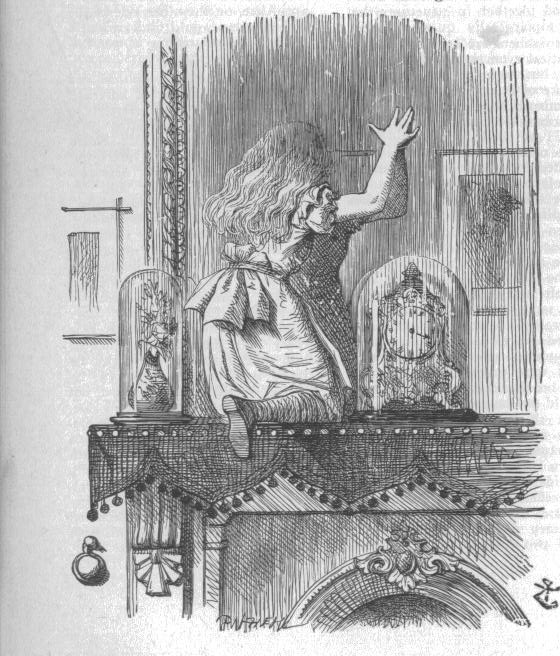
\includegraphics[width=\linewidth]{fig/intro/aliceroom.jpg}
	\caption{Looking glass room, by John Tenniel.}
\end{marginfigure}

\subsection{Conjunctive Queries}

We now turn to the $\textsf{query} \homto^? \textsf{data}$ side of the homomorphism problem. This perspective captures classical database evaluation and highlights how such queries naturally express existential, monotonic properties.
For instance, if $\?G$ is the "graph@@dir" with
two nodes $u$ and $v$ and a single edge from $u$ to $v$,
then asking if there is a "homomorphism" from $\?G$ to a graph $\?H$ amounts
to asking if there exists at least one edge in $\?G$.

As we would expect for any existential problem, they are monotonic:
if a solution exists, and we add more data, then a solution still exists.
More formally, for any "structure" $\?A$, $\?B$ and $\?B'$, if $\?B$ is a "substructure"
of $\?B'$ and $\?A \homto \?B$,
then $\?A \homto \?B'$.

The example of SQL queries (\Cref{ex:sql-as-hom}) is actually more than a mere example:
every "homomorphism problem" $\?A \homto \?B$ can be seen as a SQL query evaluation problem
where $\?A$ encodes a "query@@sem" in the \textsf{SELECT-WHERE-FROM}
fragment of SQL and $\?B$ is a relational database.
This fragment can also be characterized as the fragment
of "first-order logic" where universal quantification, union and negation are not allowed.
For instance, the SQL query of \Cref{ex:sql-as-hom} can be expressed by the formula
\begin{align*}
	\phi(\textsf{title}, \textsf{time}) \defeq\; 
	& \exists \textsf{movie\_id}.\, 
	\exists \textsf{length}.\, 
	\exists \textsf{director}.\,
	\exists \textsf{room\_id}.\, \\
	& \hphantom{\land~} \textsc{Movies}(\textsf{movie\_id}, \textsf{title}, \textsf{length}, \textsf{director}) \\
	& \land
	\textsc{Projections}(\textsf{movie\_id}, \textsf{room\_id}, \textsf{time}).
\end{align*} 
\begin{marginfigure}
	\centering
	\begin{tikzpicture}
		\node (a0) at (-.1,5.2) {};
		\node (a1) at (-.4,3.5) {};
		\node (a2) at (-.1,1.8) {};
		\node (a3) at (.1,1.8) {};
		\node (a4) at (.4,3.5) {};
		\node (a5) at (.1,5.2) {};

		\node (b0) at (-.2,5.2) {};
		\node (b1) at (-.8,3.1) {};
		\node (b2) at (-.5,1.5) {};
		\node (b3) at (-.4,.6) {};
		\node (b4) at (-.2,-.2) {};
		\node (b5) at (.2,-.2) {};
		\node (b6) at (.4,1) {};
		\node (b7) at (.2,1.4) {};
		\node (b8) at (-.5,2.6) {};
		\node (b9) at (-.4,3.8) {};
		\node (b10) at (.2,5.2) {};
	
		\draw[use Hobby shortcut, closed=true, draw=c2, fill=c2, fill opacity=.4] 
			(b0) .. (b1) .. (b2) .. (b3) .. (b4) .. (b5) .. (b6) .. (b7) .. (b8) .. (b9) .. (b10);
		\draw[use Hobby shortcut, closed=true, draw=c1, fill=c1, fill opacity=.4] 
			(a0) .. (a1) .. (a2) .. (a3) .. (a4) .. (a5);
		
		\node[vertex] at (0,5) (5) {};
		\node[vertex] at (0,4) (4) {};
		\node[vertex] at (0,3) (3) {};
		\node[vertex] at (0,2) (2) {};
		\node[vertex] at (0,1) (1) {};
		\node[vertex] at (0,0) (0) {};
		\node[font=\tiny, right=2em of 5] {\textsf{movie\_id}};
		\node[font=\tiny, right=2em of 4] {\textsf{title}};
		\node[font=\tiny, right=2em of 3] {\textsf{length}};
		\node[font=\tiny, right=2em of 2] {\textsf{director}};
		\node[font=\tiny, right=2em of 1] {\textsf{room\_id}};
		\node[font=\tiny, right=2em of 0] {\textsf{time}};

		\node[below= of 0] {output: \textsf{title}, \textsf{time}};
	\end{tikzpicture}
	\caption{
		\AP\label{fig:SQL-as-CQ}
		A "conjunctive query".
	}
\end{marginfigure}
Yet another characterization of these queries is as "conjunctive queries": such a "query@CQ"
consists of a "relational structure" together with a tuple of vertices, called ``"output@@var"''---this tuple
plays the same role as the \textsf{SELECT} statement in SQL.
For instance, the previous query can be expressed as the "conjunctive query"
of \Cref{fig:SQL-as-CQ}. The semantics of such a "query@CQ"
$\gamma = \tup{\?G, \bar x}$ is defined as follows:
given a relational database, seen as a "relational structure" $\?D$,
it returns every possible tuple $\bar d$ of elements of $\?D$ such that
there exists a "homomorphism" from $\?G$ to $\?D$ that sends $\bar x$ to $\bar d$.
Overall, these characterizations shows this fragment to be quite robust.

Hence, these problems boil down to
"homomorphism problems" of the form $\textsf{query} \homto^? \textsf{data}$.
Assuming that the "query@@sem" if fixed,
the naive algorithm to solve the "homomorphism problem"---consisting in enumerating
every possible function from $A$ to $B$ and checking whether some of them
define a "homomorphism"---works in polynomial time, as there are only $|B|^{|A|}$ such functions.
In fact, it is straightforward to devise an algorithm in "uniform-AC0"---actually, the depth
of the circuit does not even depend on $\?A$: there is roughly one layer simulating the
existential quantifiers, and another one simulating the conjunctions.

We now turn to the complexity of evaluating these "queries@CQ".
While $|B|^{|A|}$ is indeed polynomial when $\?A$ is fixed,
recall that $\?B$ represents a database:
even though complexity theory pretend that polynomial-time is tractable,
a polynomial-time algorithm of degree seven,
run over a 2.9 TB database, will execute more instructions
than there are atoms in the observable universe.
This leads to two natural questions:
\begin{itemize}
	\item optimizing the size of the exponent, "ie"
		replacing the "query@@sem" with a semantically equivalent one of smaller size,
	\item studying the parametrized complexity of the evaluating SQL queries, when parametrized by
		the size of the query. This provides a finer complexity notion than
		the classical "NP"/"AC0" approach; our previous remark shows the result to be
		slicewise polynomial ("XP"), which is not as well-behaved in practice than
		the "fixed-parameter tractable" ("FPT") problems.
\end{itemize}

\paragraph*{Query minimization.}
Both problems are in fact well-understood.
This problem of optimizing the \textsf{SELECT-WHERE-FROM} fragment of
SQL is well-understood, precisely by using the framework of "conjunctive queries"
and "relational structures".
This problem amounts to, given a "finite $\sigma$-structure" $\?A$,
deciding if there exists a strictly smaller "$\sigma$-structure" $\?A'$ "st",
for any "finite $\sigma$-structure" $\?B$, then
\[
	\?A \homto \?B
	\quad\text{"iff"}\quad
	\?A' \homto \?B.
\]
The property above is in fact equivalent to
\begin{equation}
	\?A \homto \?A'
	\quad\text{and}\quad
	\?A' \homto \?A
	\label{eq:intro-hom-equivalence}
\end{equation}
and is hence decidable.
The optimization procedure then goes as follows:
starting from $\?A$, we check for every possible vertex $a \in \?A$
if $\?A \smallsetminus \{a\}$ is equivalent to $\?A$ in the sense of
\Cref{eq:intro-hom-equivalence}. If some $a$ satisfy the property, we
let $\?A \smallsetminus \{a\}$ be our new query and start the process again.
Otherwise, we get a minimal "query@@CQ", called "core" of $\?A$.
This "core" is unique---which is not obvious since we defined it with
a greedy procedure---and is, by construction, a "substructure" of $\?A$.
In particular, it implies that the "core" does not only minimize the number of
vertices of $\?A$---while being "semantically equivalent"---, but also any
parameter that is closed under taking "substructures", such as "eg" the "tree-width".
Therefore, this notion of "core", together with seeing
\textsf{SELECT-WHERE-FROM} queries as "relational structures"/"conjunctive queries"
provides a remarkably robust tool for solving most optimization problem on these "queries@@CQ".

\begin{known}
	"Conjunctive queries" can be minimized by computing their "core".
	This process minimizes the number of vertices, but also many other
	parameters, such as "path-width", "tree-width", etc.
\end{known}

\paragraph*{FPT algorithms.}
The problem of whether a "graph@@undir" contains a "$k$-clique" easily reduces to a
"homomorphism problem" where the "input structure" is fixed---and equal to "$k$-clique".
It follows that the "homomorphism problem", parametrized in the
size of the "input structure" is "W1"-hard. Assuming that "W1" $\neq$ "FPT",%
\footnote{This is the parametrized counterpart of "P" $\neq$ "NP".}
it follows that there cannot be an "FPT" algorithm for evaluating "conjunctive queries".
This started a quest towards finding classes of "conjunctive queries" with an "FPT" evaluation.

\begin{marginfigure}
	\centering
	\begin{tikzpicture}
		\node[vertex] at (0,0) (eps) {};
		\node[vertex, below left=1.6em and 2em of eps] (a) {};
		\node[vertex, below right=1.6em and 2em of eps] (b) {};
		\node[vertex, below left=1.6em and 1.5em of a] (aa) {};
		\node[vertex, below=1.44em of a] (ab) {};
		\node[vertex, below right=1.6em and 1.5em of a] (ac) {};
		\node[vertex, below=1.44em of b] (ba) {};

		\draw[edge] (eps) to node[above left] {$\+R$} (a);
		\draw[edge] (eps) to node[above right] {$\+S$} (b);
		\draw[edge] (a) to node[above left] {$\+R$} (aa);
		\draw[edge] (a) to node[left] {$\+S$} (ab);
		\draw[edge] (a) to node[above right] {$\+T$} (ac);
		\draw[edge] (b) to node[right] {$\+R$} (ba);
	\end{tikzpicture}
	\caption{
		\AP\label{fig:intro-tree-shaped-CQ}
		A tree-shaped "conjunctive query" over a "signature"
		with three binary relations denoted by $a$, $b$ and $c$.
	}
\end{marginfigure}
First, one can notice that if said query is tree-shaped,
such as the "conjunctive query" of \Cref{fig:intro-tree-shaped-CQ}, then the naive
bottom-up evaluation algorithm works in time that is polynomial both
in the size of the query and in the size of the database.
Now, assume that $\gamma$ is a "conjunctive query" that is not necessarily
not tree-shaped, but that is equivalent to a tree-shaped "query@@CQ".
This is equivalent to saying that the "core" of $\gamma$ is "tree-shaped".
Hence, to evaluate $\gamma$, one can instead:
\begin{itemize}
	\item first compute its "core",
	\item then evaluate this "core" on the database.
\end{itemize}
The interest of this approach is that, while databases are ever-changing,
queries are often handwritten and somewhat short. Spending effort optimising them can be beneficial, since it might lead to performance gain
for \emph{every} evaluation of the query: this is why studying the
complexity of the evaluation problem parametrized by the size of
the query is relevant.
Formally, the previous procedure yields an algorithm that works in time
\[
	\+O(f(|\text{query}|) \cdot \text{poly}(|\text{core}|, |\text{database}|)).
\]
This means that evaluating "conjunctive queries" that are semantically equivalent to
tree-shaped "queries@CQ" is "FPT".

In fact, for this reasoning to work, the notion of ``tree-shaped'' need not
be as restrictive as what is shown in \Cref{fig:SQL-as-CQ}: for instance,
edges could be reversed. More generally, if the "query@@CQ" has "tree-width"%
\footnote{Tree-width is a graph-parameter that measure how far a graph is from a tree.
The notion can be extended to "relational structures".}
at most $k$, then we still get a polynomial-time evaluation algorithm---where the order
of the polynomial depends on $k$. In turns, it means that for every $k\in\Np$,
evaluating "conjunctive queries" that are semantically equivalent to
a "queries@CQ" of "tree-width" at most $k$ is "FPT".\footnote{In fact,
they can even be evaluated in polynomial time, but the argument is less straightforward
\cite{ChekuriRajaraman2000TreeWidthPolytime}.}

Remarkably, this is \emph{exactly} the limit of tractability for these "queries@CQ":
Grohe showed that a class of "conjunctive queries"
satisfying mild closure properties has "FPT" evaluation "iff"
it has bounded ``"semantic tree-width"''---meaning that there exists $k\in\Np$ "st"
every "query@CQ" in the class is "semantically equivalent" to a "query@CQ" 
of "tree-width" at most $k$ \cite{Grohe2007ComplexityHomomorphism}.%
\footnote{The same equivalent holds for polynomial-time evaluation.}

\begin{known}
	"Conjunctive queries" of bounded semantic tree-width are exactly
	the classes of "conjunctive queries" with tractable evaluation.
\end{known}


\subsection{Beyond Conjunctive Queries: Adding Regular Path Predicates for Human-Centered Data}

\begin{marginfigure}
	\centering
	\begin{tikzpicture}
		\node[vertex] at (0,2) (2) {};
		\node[vertex] at (0,1) (1) {};
		\node[vertex] at (0,0) (0) {};

		\draw[edge] (0) to (1);
		\draw[edge] (1) to (2);

		\node[font=\tiny, right=0em of 2] {\textsf{person}};
		\node[font=\tiny, right=0em of 1] {\textsf{child}};
		\node[font=\tiny, right=0em of 0] {\textsf{grand\_child}};

		\node[below= of 0] {output: \textsf{person}, \textsf{grand\_child}};
	\end{tikzpicture}
	\caption{
		\AP\label{fig:CQ-grandchild}
		A "conjunctive query" outputting all pairs of people with their grandchildren.
	}
\end{marginfigure}
Overall, the theory of \emph{conjunctive queries} is hence well-understood.
Even when considering other features from SQL, such as aggregate functions---\textsf{COUNT}, \textsf{SUM}, etc.---, the query language of "conjunctive queries" faces a big limitation:
it is \emph{intrinsically local}.
Consider two "structures" $\?A$ and $\?B$, and two elements $a$ and $a'$ of $A$.
For any homomorphism $f$ from $\?A$ to $\?B$, the "distance@@struct" from $f(a)$ to $f(a')$
in $\?B$ is at most the distance from $a$ to $a'$ in $\?A$.\footnote{This follows from
the definition of a "homomorphism", by using a trivial induction on the "distance@@struct".}
Now assume that $\?B$ is a "graph@@dir", whose vertices are humans,
and whose edges represent the `is a child of' relation.
For any $k\in\N$, it is easy to build a "conjunctive query" $\tup{\?A_k, \tup{a, a'}}$
outputting all pairs $\tup{b,b'}$ "st" $b'$ is a depth-$k$ descendant of $b$---see
\Cref{fig:CQ-grandchild} for $k=2$.
However, since "homomorphisms" contract "distances@@struct", there is no
"conjunctive query" $\tup{\?A_*, \tup{a, a'}}$ outputting all pairs $\tup{b,b'}$
"st" $b'$ is descendant, at \emph{any} depth, of $b$.
In other words, "conjunctive queries" are not closed under transitive closures.

More generally, human-centered data does not usually go well with
relational databases, as they are not designed to allow graph traversal.
To face this issue, "graph databases", also known as "knowledge graph" have
been introduced: they can essentially be modelled
as "relational structures" whose relations are all binary, "ie"
as edge-labelled graphs---see "eg" \Cref{fig:example-wikidata}.
To illustrate this point, we consider
"Wikidata", which is a knowledge graph containing more than one hundred million
vertices, whose data is used amongst others on Wikipedia. 
We would like to obtain all literary works published before 1990 and whose
French title contains the string ``exist''.
This can be done using the SPARQL query language, which is roughtly the equivalent
of SQL for knowledge bases: the query is represented in \Cref{fig:sparql,fig:sparql-explained}.
\begin{figure}
\lstinputlisting[language=SQL, morekeywords={rdfs,wd,wdt,FILTER,LANG,CONTAINS}]{fig/intro/exist.rq}
	\caption{
		\label{fig:sparql}
		A SPARQL query.\\
	\href{https://query.wikidata.org/\#SELECT\%20DISTINCT\%20\%3Fwork\%20\%3FworkLabel\%20\%3FauthorLabel\%0AWHERE\%0A\%7B\%0A\%20\%20\%3Fwork\%09wdt\%3AP31\%2Fwdt\%3AP279\%2a\%20wd\%3AQ7725634\%3B\%0A\%20\%20\%20\%20\%20\%20\%20\%20rdfs\%3Alabel\%20\%3FworkLabel\%3B\%0A\%20\%20\%09\%09wdt\%3AP577\%20\%3Fdate\%3B\%0A\%20\%20\%20\%20\%20\%20\%20\%20wdt\%3AP50\%20\%3Fauthor.\%0A\%20\%20\%3Fauthor\%20rdfs\%3Alabel\%20\%3FauthorLabel.\%0A\%20\%20FILTER\%28LANG\%28\%3FworkLabel\%29\%20\%3D\%20\%22fr\%22\%20\%26\%26\%20LANG\%28\%3FauthorLabel\%29\%20\%3D\%20\%22fr\%22\%29.\%0A\%20\%20FILTER\%28CONTAINS\%28\%3FworkLabel\%2C\%20\%22exist\%22\%29\%29.\%0A\%20\%20FILTER\%28YEAR\%28\%3Fdate\%29\%20\%3C\%3D\%201990\%29.\%0A\%7D\%0ALIMIT\%207}{[\raisebox{-.4ex}{\HandRight} Execute the query.]}
	}
\end{figure}
\begin{figure}
	\lstinputlisting[language=SQL, morekeywords={rdfs,wd,wdt,FILTER,LANG,CONTAINS}]{fig/intro/exist-bis.txt}
	\caption{
		\label{fig:sparql-explained}
		Human-friendly translation of the SPARQL query of \Cref{fig:sparql}.
	}
\end{figure}
The central notion in knowledge graphs and SPARQL is the notion of triplets:
\lstinline[language=SQL]{x R y.} refers to an edge of the \textsf{R}-relation
going from \textsf{x} to \textsf{y}.
Then \lstinline[language=SQL]{x R y; S z.} is an abbreviation for
\lstinline[language=SQL]{x R y. x S z.}
Hence, the central part (ll.~4--8) of the SPARQL query of \Cref{fig:sparql,fig:sparql-explained}
should be understood as follows:
we are looking for variables \textsf{?work}, \textsf{?typeOfWork} (implicit),
\textsf{?workLabel}, \textsf{?date} and \textsf{?authorLabel} "st":
\begin{itemize}
	\item there is a path from \textsf{?work} to \textsf{?typeOfWork}
		obtained by taking an edge `is instance of', and then an arbitrary number
		of edges of type `is subclass of',
	\item \textsf{?typeOfWork} should exactly correspond to the vertex called `type of work',
	\item \textsf{?work} has label \textsf{?workLabel}, 
	\item \textsf{?work} was published on \textsf{?date},
	\item \textsf{?work} was authored by \textsf{?author}, and
	\item \textsf{?author} has label \textsf{?authorLabel}.
\end{itemize}
They key feature of graph databases query languages is illustrated
with the \lstinline[language=SQL]{wdt : P31 / wdt : P279 *}:
this expression does not refer to a single edge of the knowledge graph,
but rather to a regular expression formed from these edges.
These regular expressions are precisely what allows for easy graph traversal!
An example of a match of this expression is provided
in red in \Cref{fig:example-wikidata}.
The output of the query of \Cref{fig:sparql,fig:sparql-explained}
is provided in \Cref{tab:output-sparql}.

\begin{figure}
	\centering
	\begin{tikzpicture}
		\node[vertex] at (0,-.5) (stats) {};
		\node[vertex] at (-1.5,-1.5) (FF) {};
		\node[vertex] at (0,-2.1) (1892) {};
		\node[vertex] at (1.5,-1.5) (French) {};
		\node[vertex] at (0,1) (bioDic) {};
		\node[vertex] at (-1.5,2) (bio) {};
		\node[vertex] at (0,2) (dico) {};
		\node[vertex] at (1.5,2) (cata) {};
		\node[vertex] at (.5,3) (kl) {};
		\node[vertex] at (-.5,3) (ref) {};
		\node[vertex] at (-1.5,3) (bioW) {};
		\node[vertex] at (-1.5,4) (nonFic) {};
		\node[vertex] at (1.5,3) (lit) {};

		\draw[edge] (stats) to node[fill=white, midway, font=\tiny] {author} (FF);
		\draw[edge] (stats) to node[fill=white, midway, font=\tiny] {date} (1892);
		\draw[edge] (stats) to node[fill=white, midway, font=\tiny] {language} (French);
		\draw[edge, draw=c0] (stats) to node[fill=white, midway, font=\tiny, text=c0] {instance of} (bioDic);

		\draw[edge, bend left, dotted] (bioDic) to (bio);
		\draw[edge, bend right, dotted] (bioDic) to (cata);
		\draw[edge, dotted, draw=c0] (bioDic) to (dico);

		\draw[edge, dotted] (bio) to (bioW);
		\draw[edge, dotted] (bioW) to (nonFic);
		\draw[edge, dotted] (cata) to (ref);
		\draw[edge, dotted] (cata) to (kl);
		\draw[edge, dotted] (dico) to (kl);
		\draw[edge, dotted] (dico) to (ref);
		\draw[edge, dotted, draw=c0] (dico) to (lit);

		\node[right=1em of stats, font=\tiny, color=cDarkGrey, text width=3.5cm]
			{"Statistique des gens de lettres et des savants existant en France@@wd"};
		\node[below left=-.25em of FF, font=\tiny, color=cDarkGrey, text width=2cm, align=right]
			{"François-Fortuné Guyot de Fère@@wd"};
		\node[below=-.25em of 1892, font=\tiny, color=cDarkGrey]
			{1892};
		\node[below right=-.25em of French, font=\tiny, color=cDarkGrey]
			{"French@@wd"};
		\node[below left=-.5em and 1em of bioDic, font=\tiny, color=cDarkGrey, text width=1.5cm, align=right]
			{"biographical dictionary@@wd"};
		\node[left=-.25em of bio, font=\tiny, color=cDarkGrey]
			{"biography@@wd"};
		\node[below right=-.25em and -.25em of dico, font=\tiny, color=cDarkGrey]
			{"dictionary@@wd"};
		\node[right=-.25em of cata, font=\tiny, color=cDarkGrey]
			{"catalogue@@wd"};
		\node[above=.25em of kl, font=\tiny, color=cDarkGrey, text width=2cm, align=center]
			{"knowledge organization system@@wd"};
		\node[above=-.25em of ref, font=\tiny, color=cDarkGrey]
			{"reference work@@wd"};
		\node[left=-.25em of bioW, font=\tiny, color=cDarkGrey]
			{"biographical work@@wd"};
		\node[left=-.25em of nonFic, font=\tiny, color=cDarkGrey]
			{"non-fiction work@@wd"};
		\node[right=-.25em of lit, font=\tiny, color=cDarkGrey]
			{"literary work@@wd"};
	\end{tikzpicture}
	\caption{
		\AP\label{fig:example-wikidata}
		Part of the "Wikidata" knowledge graph.
		Dotted arrows represent the relation `subclass of'.
		The red path matches the expression \lstinline[language=SQL]{wdt : P31 / wdt : P279 *}.
		For readability, labels are written next to the vertices
		rather than as separate vertices linked with a `has label' relation.
	}
\end{figure}
\begin{table}
	\centering
	{
		\footnotesize%
		\begin{tabular}{ll}
			\toprule
			workLabel & authorLabel \\ \midrule 
			Statistique des gens de lettres 
				& \multirow{2}{*}{François-Fortuné Guyot de Fère}\\
			et des savants existant en France
				& \\
			Le Chevalier inexistant
				& Italo Calvino\\
			L'existentialisme est un humanisme
				& Jean-Paul Sartre\\
			Ennui existentiel
				& Anton Tchekhov\\
			Les Ennuis de l'existence
				& Anton Tchekhov\\
			La tentation d'exister
				& Emil Cioran\\
			Inexistence
				& David Zindell \\ \bottomrule
		\end{tabular}
	}
	\caption{
		\AP\label{tab:output-sparql}
		Output of the SPARQL query of \Cref{fig:sparql,fig:sparql-explained}.}
\end{table}

We formalize the core features of SPARQL as "conjunctive regular path queries":
they consist of "conjunctive queries", except that their atoms are no
longer of the form $x \atom{\+R} y$ (for some binary relation $\+R \in \sigma$),
but can be more generally of the form
\[
	x \atom{L} y
	\quad\text{ for some "regular language" $L$ over $\sigma$}.
\]
For instance, ll.~1--8 of the SPARQL query of \Cref{fig:sparql,fig:sparql-explained}
can be modelled by the "conjunctive regular path query" of \Cref{fig:intro-SPARQL-as-CRPQ}:
notice the regular expression in red.
\begin{marginfigure}
	\centering
	\begin{tikzpicture}
		\node[vertex] at (0,0) (work) {};
		\node[vertex, above=3em of work] (litWork) {};
		\node[vertex, below left=2.2em and 2.7em of work] (workLabel) {};
		\node[vertex, below=2.9em of work] (date) {};
		\node[vertex, below right=2.2em and 2.7em of work] (author) {};
		\node[vertex, below=2.5em of author] (authorLabel) {};

		\draw[edge] (work) to node[fill=white, font=\tiny, text=c0] {instance $\cdot$ subclass${}^*$} (litWork);
		\draw[edge] (work) to node[fill=white, font=\tiny] {label} (workLabel);
		\draw[edge] (work) to node[fill=white, font=\tiny] {date} (date);
		\draw[edge] (work) to node[fill=white, font=\tiny] {author} (author);
		\draw[edge] (author) to node[fill=white, font=\tiny] {label} (authorLabel);

		\node[right=-.25em of work, font=\tiny, color=cDarkGrey]
			{work};
		\node[right=-.25em of litWork, font=\tiny, color=cDarkGrey]
			{typeOfWork};
		\node[left=-.25em of workLabel, font=\tiny, color=cDarkGrey]
			{workLabel};
		\node[below=-.25em of date, font=\tiny, color=cDarkGrey]
			{date};
		\node[right=-.25em of author, font=\tiny, color=cDarkGrey]
			{author};
		\node[right=-.25em of authorLabel, font=\tiny, color=cDarkGrey]
			{authorLabel};

		\node[below=4.5em of date] {output: \textsf{workLabel}, \textsf{authorLabel}};
	\end{tikzpicture}
	\caption{
		\AP\label{fig:intro-SPARQL-as-CRPQ}
		A "conjunctive regular path query" 
		modelling the core part of \Cref{fig:sparql,fig:sparql-explained}.
	}
\end{marginfigure}

\begin{known}
	"Graph databases"/knowledge graphs store information as edge-labelled graphs.
	To allow for graph traversal, we extend "conjunctive queries"
	to "conjunctive regular path queries" by adding regular expressions.
\end{known}


\subsection{Minimization and Structure of Conjunctive Regular Path Queries}

While "conjunctive regular path queries" share some enjoyable properties
of "conjunctive queries"---for instance the decidability of "semantical equivalence",
in contrast to "eg" "first-order logic"---its semantics is more complex:
graph-like phenomenon ("homomorphisms") intertwines with "regular languages".
Not only does this lead to a complexity blow-up---"semantical equivalence" is "NP"-complete
for "conjunctive queries" but "ExpSpace"-complete for "conjunctive regular path queries"---,
it also breaks the nice theory of "cores".

As a consequence, the optimizing "conjunctive regular path queries" poses
a significant challenge to untwist graph properties from automata-theoretic ones.
This first part of this thesis is dedicated to this problem.
After exposing the basic theory of "conjunctive regular path queries"
in \Cref{ch:prelim-graph-databases}, we study
the "minimization problem@@CRPQ" in \Cref{ch:minimization-CRPQ}:
given such a "query@CRPQ" and $k\in\Np$, we can decide if it is equivalent to a "query@CRPQ"
of size at most $k$, and if so we can produce it.

\begin{contribution}
	Whether a "conjunctive regular path query" can be minimized is decidable,
	and minimization is effective.
\end{contribution}

We notice that, somewhat unexpectedly, there are some "conjunctive regular path queries"
that are minimal in the sense above, but that are equivalent to a \emph{finite union}---in the 
semantical sense---of strictly smaller "conjunctive regular path queries".%
\footnote{This contrasts with the case of "conjunctive queries",
where the notion of "core" and the order-theoretic properties
of "relational structures" precisely prevents this phenomenon from appearing.
In other words, this phenomenon precisely emerges by interlacing
the graph structure and the automata of the "query@@CRPQ".}
We argue that measuring a union of such "queries@@CRPQ" by the maximal size
of a query in the union is a sensitive thing to do---because the complexity
of evaluating such a union depends mostly on this parameter---, and prove
that given a "conjunctive regular path queries" and $k\in\N$, we can
decide if it is equivalent to a finite union of
"queries@CRPQ" which are all of size at most $k$.

\begin{contribution}
	Whether a "conjunctive regular path query" can be minimized
	as a union of strictly smaller "queries@@CRPQ" is decidable,
	and minimization is effective.
\end{contribution}

Both algorithms are essentially brute-force, and the main technical difficulty
lies in proving that finitely many candidates to test, which is not
trivial because we do not ask for any bound on the size of the "regular languages".%
\footnote{Again, the motivation lies from the fact that the complexity of evaluating
a "conjunctive regular path queries" mostly depends on how many "atoms"/edges it has,
and not so much on how complex these languages are.}
The idea behind the two algorithms are in fact surprisingly different:
\begin{itemize}
	\item in the first case---when union is not allowed---, we prove that
		if a "query@CRPQ" is equivalent to another one with few
		"atoms" (but potentially big languages), then it must be
		equivalent to a "query@CRPQ" with few "atoms" \emph{and} small languages.
		This property is proved by understanding the subtle interactions between
		languages and the graph structure;
	\item in the second case---when union is allowed---, we build a canonical
		finite union of "queries@CRPQ", corresponding to the
		"maximal under approximation" by a finite union of small "queries@CRPQ": 
		it is the \emph{best} under approximation---in the sense that
		it logically entails the "query@CRPQ"---and so, if the original
		"query@CRPQ" is equivalent to a finite union of small ones, then
		it must be equivalent to this "maximal under approximation".
		The difficulty there lies in proving the existence of "maximal under approximation",
		or rather that it can be expressed by a \emph{finite} union.
		This construction can essentially be seen as a
		smart brute-forcing, obtained by agglomerating all possible smaller "queries@CRPQ".
\end{itemize}

One reason we resolve to using brute-force algorithm is that it is
remarkably hard to understand when a "query@CRPQ" cannot be minimized.
The case of "conjunctive queries" is much simpler: if the "core" 
of the "query@CQ" has $k$ edges (resp. "tree-width" $k$),
then any "conjunctive query" "semantically equivalent" to it must use at least $k$ edges
(resp. have "tree-width" at least $k$).
Another of our contributions is to identify a sufficient condition%
\footnote{However, contrary to the "core", this condition is not necessary.}
on a "query@CRPQ" so that \emph{any} "query" "semantically equivalent" to it
must contain a ``complex pattern''. The strength of this theorem lies in its
general applicability, as the notion of ``complex pattern''
is formalized as a ``"minor-closed" class
of graphs''---examples include the class of all graphs with at most $k$ "atoms",
or the class of all graphs of "tree-width" at most $k$.

\begin{contribution}
	We introduce the "semantical structure theorem", that provides
	a way to prove lower bounds on the number
	of "atoms", or "tree-width", or any minor-closed property,
	that is necessary to express a "query@@sem".
\end{contribution}

This tool proves useful to prove minimality of specific examples---"ie"
for proofs---, and to prove complexity lower bounds for our problem.
However, this it only provides a sufficient condition, that is often not
necessary, it fails to provide a \emph{simple} algorithm to test minimality---hence our
brute-force algorithms.

Then, in \Cref{ch:semantic-tree-width-CRPQ}, we turn to the question
of "tree-width". Similarly to "conjunctive queries", finite unions of
"conjunctive regular path queries"
of bounded "tree-width" can be evaluated in polynomial time.
It begs the question of deciding when a "query@CRPQ" is actually equivalent
to such an object.

\begin{known}
	Barceló, Romero and Vardi \cite{BarceloRomeroVardi2016SemanticAcyclicity}
	devised an algorithm to test
	if a "conjunctive regular path queries" is equivalent to
	a finite union of ``acyclic''---meaning of "tree-width" 1---"queries@CRPQ".
\end{known}

Unfortunately, the general question for "tree-width" $k$ is left open at the end
of their paper as the authors did not know how to extend their technique to this
more general setting. We extend their result, relying again on the notion
of "maximal under-approximation":%
\footnote{The paper of Barceló, Romero and Vardi
also relies on "maximal under-approximations", and this notion already existed
for "conjunctive queries".}
we prove that, given a "conjunctive regular path query" and
$k\in\Np$ the existence and computability of its "maximal under-approximation"
by finite unions of "queries@CRPQ" of "tree-width" at most $k$.

\begin{contribution}
	Given $k\in \Np$ and a "conjunctive regular path queries",
	we can decide if the latter is "semantically equivalent"
	to a finite union of "queries@CRPQ" of "tree-width"
	(resp. "path-width") at most $k$.
\end{contribution}

The proof of existence of this "maximal under-approximation" is
actually quite hard---at least much harder than in the case minimizing
the number of "atoms"---as it needs to deal with two kind of information:
the structure of the query, "ie" its underlying graph, and its languages.
The proof precisely massages the query to, at the same time,
preserve information about the "tree decomposition"---serving as a
witness of the small "tree-width" of the "query@CRPQ"---and about the
semantics of the "query@CRPQ".

Amusingly, we originally thought that our proof was not able to
capture the case $k=1$ that was already handled, and that the constructions
of Barceló, Romero and Vardi and ours were orthogonal.
When written the journal version of this paper---that was originally
published at ICDT '23---, we wanted to extend the results to "path-width",%
\footnote{The main motivation behind this is that the evaluation of "queries@CRPQ"
of bounded "path-width" is not only polynomial but even "NL"!}
but part of our construction broke. Introducing the technical tool
to fix it\footnote{See the notions of "contractions" and "contracted path-width".}
actually leads to a unified solution, that handles both
the case of "tree-width" $k$ (including $k=1$) and "path-width".%
\footnote{Lastly, note that the order of presentation of these results
does not follow the timeline of their discovery: our work on "semantic tree-width"
was done in 2022--23 and published at ICDT '23, while the one on minimization
was done in 2024--25 and published at PODS '25.}

Lastly, all these algorithms relies on testing the equivalence
of "conjunctive regular path queries", which is "ExpSpace".
It leads to resource-hungry algorithms,%
\footnote{Although it has to be noted that it is worth running exponential
algorithm on smallish "queries@CRPQ" in order to optimize
its evaluation on huge databases!}
which leads to a natural quest for identifying subclasses
of "queries@CRPQ" that admit more efficient algorithms.

"Conjunctive regular path queries" over "simple regular expression",
where the "regular languages" allowed are restricted to be concatenations of
edge-labels and reflexive-transitive closure ("aka" Kleene star) of
edge-labels, were already known to have a more efficient
algorithm for testing "semantical equivalence".

\begin{contribution}
	We prove that the problem of minimizing the number of "atoms" (resp. "tree-width")
	of "conjunctive regular path queries" over "simple regular expression"
	lies in the polynomial hierarchy.
\end{contribution}

A consequence of our work on "tree-width" is that,
given a "conjunctive regular path query" that is promised to be equivalent
to a "query@CPRQ" of "tree-width" $k$, we can first compute said
equivalent query of small "tree-width" by using our algorithm,
and then evaluate it on any database. This proves that the evaluation
problem for "conjunctive regular path queries" of bounded "semantic tree-width"
is "FPT" when parametrized by the size of the "query@@sem".%
\footnote{This result was in fact already known---but proven differently, with
an incomparable complexity (better preprocessing but worst polynomial exponent)---by
Romero, Barceló and Vardi \cite{RomeroBarceloVardi2017Homomorphism}.}

Whether the converse hold remains a mystery: many attempts
have been tried to extend Grohe's proof for "conjunctive queries" to this setting,
but all failed, precisely because of the difficulty posed
by the intertwining of the graph structure and the automata.
We conclude this part of the thesis by a discussion of this problem,
as well as whimsical ideas related to "conjunctive regular path queries"
in \Cref{ch:conclu-database}.

\begin{openproblemintro}
	Characterize the "classes of CRPQ" with "FPT" evaluation
	when parametrized in the size of the "query@CRPQ".
\end{openproblemintro}

To summarize, the $\textsf{query} \homto^? \textsf{data}$ formulation of the "homomorphism problem" provides a robust foundation for classical database theory. The first part of this thesis extends this framework to a richer context: graph databases and queries extended with regular path predicates.
\section{Everyone Who Wants to Do Constraint Satisfaction Always Ends in Universal Problems}
% Everyone who wants to do good to the human race always ends in universal bullying.
% - Aldous Huxley
\label{sec:intro-universal}

\subsection{Constraint Satisfaction Problems}

This second part explores the complexity of the "homomorphism problem" when the data is fixed and the query varies, focusing on "constraint satisfaction problems" and "automatic structures".

\begin{marginfigure}[-15em]
	\centering
	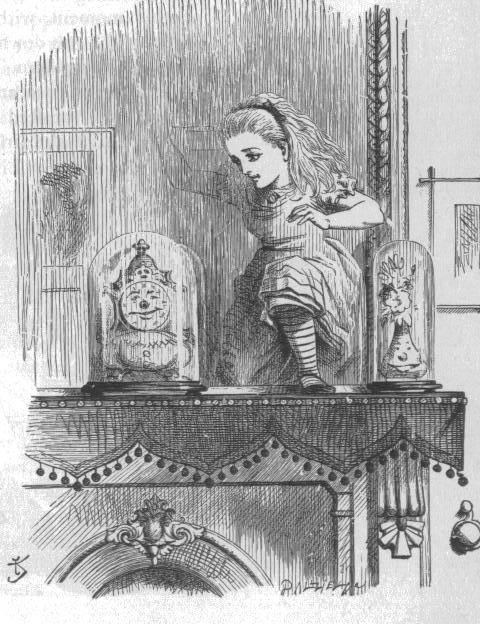
\includegraphics[width=\linewidth]{fig/intro/aliceroom2.jpg}
	\caption{Looking glass room, by John Tenniel.}
\end{marginfigure}

\paragraph*{Constraint Satisfaction Problems.}
Going to the other side, encodings of model-checking problems
as "homomorphism problems" of the form $\textsf{data} \homto^? \textsf{query}$
can be thought of as ``universal problems''---here ``universal'' does not
refer to some form of completeness, but simply to universal quantification.
Notice "eg" that they are anti-monotonic with respect to the data:
for all "structures" $\?A$, $\?A'$ and $\?B$, if $\?A \homto \?B$ and $\?A'$ is a substructure
of $\?A$ then $\?A' \homto \?B$.
Moreover, while problems of the form $\textsf{query} \homto^? \textsf{data}$
can be solved locally---whether a vertex of the data is part of a solution (a "homomorphism") only 
depends on its "neighbourhood"---, problems of type $\textsf{data} \homto^? \textsf{query}$ cannot.

\begin{marginfigure}[-18em]
	\centering
	\begin{tikzpicture}
		% ---
% 3-clique
% ---
\node[vertex, draw=c0, fill=c0, fill opacity=.4] at (0,0) (k3-0) {};
\node[vertex, above right=1em and 2em of k3-0, draw=c1, fill=c1, fill opacity=.4] (k3-1) {};
\node[vertex, below right=1em and 2em of k3-0, draw=c2, fill=c2, fill opacity=.4] (k3-2) {};

\draw[edge, bend right=15] (k3-0) to (k3-1);
\draw[edge, bend right=15] (k3-0) to (k3-2);
\draw[edge, bend right=15] (k3-1) to (k3-0);
\draw[edge, bend right=15] (k3-1) to (k3-2);
\draw[edge, bend right=15] (k3-2) to (k3-0);
\draw[edge, bend right=15] (k3-2) to (k3-1);
	\end{tikzpicture}
	\caption{
		\AP\label{fig:intro-3-clique}
		The "$3$-clique" $\clique{3}$.
	}
\end{marginfigure}
\begin{marginfigure}[-6em]
	\centering
	\begin{tikzpicture}
		% ---
% Example 3-colouring
% ---
\tikzset{every node/.style={fill opacity=.4}}
\node[vertex, color=c0, fill=c0] at (0,0) (0) {};
\node[vertex, above left=.75em of 0, color=c1, fill=c1] (0al) {};
\node[vertex, above right=.75em of 0, color=c2, fill=c2] (0ar) {};
\node[vertex, below left=2em of 0al, color=c0, fill=c0] (0l) {};
\node[vertex, below right=2em of 0ar, color=c0, fill=c0] (0r) {};
\node[vertex, above left=of 0l, color=c1, fill=c1] (0ll) {};
\node[vertex, above right=of 0r, color=c2, fill=c2] (0rr) {};
\node[vertex, below left=of 0, color=c2, fill=c2] (0bl) {};
\node[vertex, below right=of 0, color=c1, fill=c1] (0br) {};

\node[vertex, below=2em of 0, color=c0, fill=c0] (1) {};
\node[vertex, below left=1em of 1, color=c1, fill=c1] (1bl) {};
\node[vertex, below right=1em of 1, color=c2, fill=c2] (1br) {};
\node[vertex, above left=0em and 1.5em of 1bl, color=c2, fill=c2] (1bll) {};
\node[vertex, above right=0em and 1.5em of 1br, color=c1, fill=c1] (1brr) {};

\node[vertex, below=4em of 1, color=c0, fill=c0] (2) {};
\node[vertex, below left=1.5em and .75em of 1bl, color=c2, fill=c2] (2al) {};
\node[vertex, below right=1.5em and .75em of 1br, color=c1, fill=c1] (2ar) {};
\node[vertex, below left=.5em and 1.5em of 2, color=c1, fill=c1] (2bl) {};
\node[vertex, below right=.5em and 1.5em of 2, color=c2, fill=c2] (2br) {};
\node[vertex, below left=of 2al, color=c0, fill=c0] (2ll) {};
\node[vertex, below right=of 2ar, color=c0, fill=c0] (2rr) {};

\draw[edge] (0) to (0al);
\draw[edge] (0) to (0ar);

\draw[edge] (0al) to (0l);
\draw[edge] (0l) to (0bl);
\draw[edge] (0bl) to (0);
\draw[edge] (0l) to (0ll);

\draw[edge] (0ar) to (0r);
\draw[edge] (0r) to (0br);
\draw[edge] (0br) to (0);
\draw[edge] (0r) to (0rr);

\draw[edge] (0bl) to (1);
\draw[edge] (1) to (1bl);
\draw[edge] (1bl) to (0l);

\draw[edge] (0br) to (1);
\draw[edge] (1) to (1br);
\draw[edge] (1br) to (0r);

\draw[edge] (1bl) to (2al);
\draw[edge] (2al) to (2ll);
\draw[edge] (2) to (2al);
\draw[edge] (2) to (2bl);
\draw[edge] (2bl) to (2al);

\draw[edge] (1br) to (2ar);
\draw[edge] (2ar) to (2rr);
\draw[edge] (2) to (2ar);
\draw[edge] (2) to (2br);
\draw[edge] (2br) to (2ar);

\draw[edge] (1bl) to (1bll);
\draw[edge] (1br) to (1brr);

\draw[edge, bend right=20] (2) to (1bl);
\draw[edge, bend left=20] (2) to (1br);


	\end{tikzpicture}
	\caption{
		\AP\label{fig:dichotomy-ex-3-clique}
		A "$3$-colouring" of some beetle-shaped "graph@@dir".
	}
\end{marginfigure}
\begin{example}[Graph colouring]
	\AP\label{ex:graph-colouring-as-hom}
	Let $k\in\Np$. We let the \AP""$k$-clique"", denoted by $\intro*\clique{k}$,
	to be the "graph@@dir" whose vertices are $\lBrack 1,k\rBrack$,
	and with an edge from $i$ to $j$ (with $i,j \in \lBrack 1,k\rBrack$)
	"iff" $i\neq j$, see \Cref{fig:intro-3-clique}.
	We say that a finite "graph@@dir" $\?G$ is \AP""$k$-colourable"" when
	we can map every vertex of $\?G$ to an element of $\lBrack 1,k\rBrack$
	"st" no two adjacent vertices are sent on the same colour/number.
	In other words, a $k$-colouring corresponds precisely to a "homomorphism" from $\?G$
	to $\clique{k}$, where colours correspond to the vertices of the clique,
	see "eg" \Cref{fig:dichotomy-ex-3-clique}.
	Hence, a graph is "$k$-colourable" if, and only if,
	there is a "homomorphism" from $\?G$ to $\clique{k}$.
\end{example}

For instance, "$3$-colourability" is a global property of a graph and cannot be solved
by gluing local solutions. In particular, this implies that fixing the query
does not necessarily result in
a drop in the complexity: "$3$-colourability" is already "NP"-complete!
The next example shows that, even when the "target structure" is fixed, the "homomorphism problem"
provides a flexible framework to encode problems.

\begin{example}[SAT solving]
	\AP\label{ex:sat-as-hom}
	We consider a 3-SAT instance, namely a finite conjunction of
	disjunctions of three literals, say
	\[
		\phi \defeq \bigwedge_{i=1}^n \ell_{i,1} \lor \ell_{i,2} \lor \ell_{i,3},
	\]
	where each $\ell_{i,j}$ is either a variable, or the negation of a variable.
	We assume "wlog" that in each clause, positive variables appear before negative ones:
	this of course can be achieved by a simple syntactical rewriting of each clause.%
	\footnote{Meaning "eg" that $x \lor \neg y \lor z$ is not allowed, contrary to
	$x \lor z \lor \neg y$.}
	We let $\?B$ be the structure whose domain has two elements $\{0,1\}$,
	equipped with four ternary relations $\+R_0$ through $\+R_3$, where $\+R_j$ encodes clauses with exactly $j$ negated literals. They are formally defined as
	\begin{align*}
		\+R_0 & \defeq \set{0,1}^3 \smallsetminus \set{\tup{0,0,0}}, &
		\+R_1 & \defeq \set{0,1}^3 \smallsetminus \set{\tup{1,0,0}}, \\
		\+R_2 & \defeq \set{0,1}^3 \smallsetminus \set{\tup{1,1,0}} \qquad\text{ and} &
		\+R_3 & \defeq \set{0,1}^3 \smallsetminus \set{\tup{1,1,1}}.
	\end{align*}
	We then encode $\phi$ into the "relational structure" $\?F_\phi$
	whose domain is the set of variables of $\phi$,
	and for every $i \in \lBrack 1,n \rBrack$,
	$\+R_j$ ($j\in\lBrack 0,3\rBrack$) consists of all triplets of variables $\tup{x,y,z}$
	"st" there is a clause of $\phi$ containing variables $x$, $y$ and $z$ (with multiplicity), and exactly $j$ of these variables occur negatively.
	For instance, $\tup{x, y, \neg x} \in \+R_1$, and $\tup{\neg x, \neg y, \neg z} \in \+R_3$.
	A function $f$ from the domain of $\?F_\phi$ to the domain of $\?B$ amounts to picking
	a Boolean valuation of the variables occurring in $\phi$.
	Observe that, by definition of the relations $\+R_j$,
	given a clause $\psi$ containing variables $x,y,z$, 
	$f$ is a "homomorphism" from $\?F_\psi$ to $\?B$ "iff"
	$f$, seen as a valuation, satisfies $\psi$.\footnote{For instance,
	if all variables are positive, then all valuations except the one putting
	all variables to false satisfy the formula. This is why $\+R_0$ is defined
	on $\?B$ as $\set{0,1}^3\smallsetminus \set{\tup{0,0,0}}$.}
	By taking conjunction, the conclusion follows: "homomorphisms" from
	$\?F_\phi$ to $\?B$ exactly correspond to valuations satisfying $\phi$.
	In particular, there is a "homomorphism" from $\?F_\phi$ to $\?B$ "iff"
	$\phi$ is satisfiable.%
	\footnote{Note that this example can be easily generalized to $k$-SAT for any $k\in\Np$.
	However, the "signature" depends on $k$.}
\end{example}

However, contrary to "$3$-colourability" and SAT solving, not all of these problems are NP-hard. For example, $2$-colourability is not only polynomial-time,
but can be solved using a greedy algorithm. This begs the question of understanding what
makes a "relational structure" hard for the "homomorphism problem" when it is used
as the "target structure".
This question is not only motivated by theory: constraint logic programming has emerged in the 1980s
with Prolog II and III; and modern programming languages such as answer-set programming provide an 
efficient was of doing constraint solving.

\begin{figure}
	\centering
	\lstinputlisting[language=Prolog, breaklines=true]{fig/intro/sudoku.lp}
	\caption{
		\AP\label{fig:ex-sudoku-asp}
		A Clingo program (answer-set programming) to solve Sudoku grids.
		Written by Enrico Höschler
		\href{https://ddmler.github.io/asp/2018/07/10/answer-set-programming-sudoku-solver.html}{[source]}.
		Try running it on \url{https://potassco.org/clingo/run/}!
	}
\end{figure}

Answer-set programming can be thought of, albeit caricaturally, as a human-readable
SAT-solver. It deals with variables, relations between these variables,
and logical rules between these variables. These rules take the form
\lstinline|A :- B|, which can be understood as `if $B$, then $A$'.
The right-hand side is parsed conjunctively while the left-hand side is parsed disjunctively:
\lstinline|A, B :- C, D| should be understood as `if $C$ and $D$, then $A$ or $B$'.
\Cref{fig:ex-sudoku-asp} provides
an example of a Clingo program for solving Sudoku grids:
\begin{itemize}
	\item it starts by declaring three types of variables: absissa $x$, ordinates $y$ and values $n$ (representing a value in the grid), as well as their range;
	\item it introduces a \textsf{sudoku} ternary relation, where $\textsf{sudoku}(x,y,n)$
		represents the fact that entry $(x,y)$ of the grid has value $n$,
		and it says that there should be exactly one value per entry;
	\item it introduces a \textsf{subgrid} relation, saying when two entries
		belong to the same 3$\ast$3-square;
	\item finally, it says that any two values on the same column, row or subgrid
		must be different.%
		\footnote{Recall that the left-hand side of rules is understood disjunctively,
		and hence \lstinline|:- A, B| reads as `if $A$ and $B$, then false'.}
\end{itemize}
To solve a specific grid using the program of \Cref{fig:ex-sudoku-asp},
it suffices to add declarations of the form \lstinline|sudoku(4,1,5).|,
where \lstinline|A.| is a shorthand for \lstinline|A :-.|.
This specifies that the cell at position $(4,1)$ has value 5.

Contrary to more classical programming languages, this paradigm does not explain \emph{how} things
should be computed, but \emph{what constraints} the memory/solution should satisfy.
In "homomorphism problems", the "target structure" precisely plays this role of
encoding constraints. For instance, the only constraint for a graph $3$-colouring is that
adjacent vertices must be mapped to distinct colours: this constraint is
reflected in $\clique{3}$ by the fact that the edges of $\clique{3}$ are exactly the pairs
of distinct colours.

The field of \emph{constraint satisfaction problems} precisely aims at classifying the
structures $\?B$ "wrt" to the complexity of the "homomorphism problem" when the
"target structure" is $\?B$. One of the earliest and most impactful result
of the domain was found by Schaefer \cite{Schaefer1978ComplexitySatisfiability},
who proved that such problems are either in "P" or "NP"-complete when the domain of $\?B$
has two elements---this already captures the example of SAT-solving (\Cref{ex:sat-as-hom}) from earlier.
A decade later, Hell and Ne\v{s}et\v{r}il \cite{HellNesetril1990ComplexityColoring}
proved a similar result for undirected graph.
Moreover, in both cases, these dichotomies are effective: given a structure, we can decide if
its "homomorphism problem" is in "P" or is "NP"-complete.
These results, together with the importance of \emph{constraint satisfaction} in computer science
lead Feder and Vardi at the end of the 1990s
to state their infamous \emph{dichotomy conjecture}: ``for any "finite structure" $\?B$,
the "homomorphism problem" with "target structure" $\?B$ is either "P"
or "NP"-complete'' \cite{FederVardi1998ComputationalStructure}.
Despite receiving lots of attention, the conjecture remained wide open for two decades, until
Bulatov \cite{Bulatov2017DichotomyCSPs} and Zhuk \cite{Zhuk2020CSPDichotomy} independently
showed the conjecture to be true.%
\footnote{Both papers have in fact been first published in 2017 in the same conference:
\cite{Zhuk2020CSPDichotomy} refers to Zhuk's later journal version.}

However not all problems in "P" are complete for this class: some are even simpler and are complete
for "NL" or "L", or even "FOfin"---i.e. it is a "first-order definable" class of "finite structures".
One result that will be of major importance in this thesis is a dichotomy
theorem by Larose and Tesson separating "structures" in "FOfin" from those that are "L"-hard
\cite{LaroseTesson2009UniversalAlgebraCSP}.

\begin{known}
	The field of constraint satisfaction problems classifies "target structures"
	depending on the complexity of their "homomorphism problem".
\end{known}

\subsection{Automatic Structures: The Dream Is Not Over Yet}

The second part of this thesis is dedicated to pushing these results to their limit.
The "structures" handled by the "homomorphism problem", like most
problems in computer science, are usually assumed to be "finite@@struct".
We discuss in this section the generalization of the problem to
infinite structures. This motivated by two facts: not only infinite structures
naturally arise as from computational models---the runs of a machine
usually form an infinite "structure"---, they can also model `mathematical universes'.

Von Neumann would have said ``It's all over''%
\footnote{This quote is claimed to be historically accurate by
\cite{2009Logicomix}, however this claim seems undocumented \cite{Mancosu2011Logicomix}.}
after hearing Gödel expose his infamous "incompleteness theorem" in 1930:
any \emph{effective} (recursively enumerable)
consistent theory that is expressive enough to express the arithmetic
is incomplete---"ie" it contains statements that are neither valid (true in all models),
nor unsatisfiable (false is all models).
In other words, there is no reasonable set of axioms
to capture all mathematics: some statements must necessarily fall outside
the scope of the theory.

Completeness is perhaps best understood as follows:
if a theory (a set of axioms) is consistent---"ie" it has at least one model---and complete, 
then pick any of its model. A statement is then valid in the theory if and only
if it is true in this model. Dually, if you are given a theory for which
there exists a model with this property (a statement is valid in the theory "iff" it
is true in the model), then the theory is complete.
In essence, not only does Gödel's puts a dent in Hilbert's dream
(``Wir müssen wissen. Wir werden wissen.'') of building solid foundations for mathematics:
in fact, it shatters the Platonistic idea of an unequivocal \& universal mathematical world, or 
at the very least of one that can be captured by axioms.

Ironically, what makes "Gödel's incompleteness theorem" a proper
abomination  for computer scientists is probably Gödel's own theorem, that he proved only a year before, in his
Ph.D. dissertation, known as "Gödel's completeness theorem": 
first-order logic admits a complete proof system. Or, said differently,
what is valid---that is, true on every model satisfying the axioms---is exactly what
can be proven. 
Hence, the Gödel of 1929 could have dreamt of a complete theory for mathematics.
If a such theory existed, to determine if a statement $\phi$ was valid, it would suffice
to enumerate in parallel all possible proofs of $\phi$ and of $\neg \phi$. By completeness, this 
procedure would always stop, and either conclude that $\phi$ is valid, or that
$\neg \phi$ is valid.%
\footnote{Formally: any recursively enumerable complete first-order theory is decidable.}
Are there cardinals strictly between $\aleph_0$ and the continuum?
Start Turing's nifty device---invented in 1936---, and you would (eventually) get an answer! In this strange world, automatic theorem proving would be a reality,
and this thesis would probably look very different.

Sadly for the Gödel of 1929, the Gödel of 1930 came, and so… ``It's all over''!
Since then, theories---such has
"Zermelo–Fraenkel set theory plus the axiom of choice"---have been developed, and while not being complete, they 
manage to capture most of the parts of mathematics we are interested in.%
\footnote{For the sake of sanity, we assume
throughout this introduction that the pronoun `we' excludes set theorists.}
\begin{marginfigure}
	\centering
	\[
	\contraction{}{\tau\,}{{\vee} {\neg} {\in}}{\!\square}
	\contraction[2ex]{}{\tau\!}{{\vee} {\neg} {\in} \square A' {\in}}{\square}
	\tau {\vee} {\neg} {\in} \square A' {\in} \square A''
	\]
	\caption{\AP\label{fig:intro-bourbaki}
	The "first-order sentence" $\exists x.\, (x \not\in A') \lor (x \in A'')$
	as written by Bourbaki in \cite[\S~1]{Bourbaki2006Logique}.
	}
\end{marginfigure}
\begin{marginfigure}
	\centering
	\[
		\Fanqn{x}\Fconditional{\Fcontent x \in A''}{\Fcontent x \in A'}
	\]
	\caption{\AP\label{fig:intro-frege}
		The "first-order sentence" of \Cref{fig:intro-bourbaki}
		written using Frege's notations (1879).
	}
\end{marginfigure}
Yet, after half a century of efforts to build solid foundations,
the incompleteness of this consolation prize is actually frustrating,
and mathematicians still often resort to denial.
\begin{displayquote}[Jean Dieudonné {\cite{Dieudonne1970Bourbaki}}]
	``On foundations we believe in the reality of mathematics, but of course when philosophers attack us with their paradoxes we rush to hide behind formalism and say: ``Mathematics is just a combination of meaningless symbols,'' and then we bring out Chapters 1 and 2 on set theory. Finally we are left in peace to go back to our mathematics and do it as we have always done, with the feeling each mathematician has that he is working with something real.
	This sensation is probably an illusion, but is very convenient. That is Bourbaki's attitude towards foundations.''
\end{displayquote}
For the reader intrigued by what could possibly frighten philosophers in Bourbaki's first volume,
we refer them to the formula of \Cref{fig:intro-bourbaki}---interestingly, this is not the most 
frightening way to write formulas, see \Cref{fig:intro-frege}!

However, not all hope is lost: while the Platonistic mathematical world might
not be understood, some of it restrictions might be axiomatized.
In 1929, Presburger proved that a natural set of axioms for doing
arithmetic with only addition is also both complete and decidable---the formulas
that are valid in this theory exactly correspond to the sentences that are true on $\tup{\N,+}$.
Around the same time, Tarski formalized Euclide's geometry as a first-order theory, and proved
that is was complete and decidable, see \cite{TarskiGivant1999Geometry}.

Hence, logic is not completely useless at capturing complex infinite structures!
Interestingly, generalizing the idea behind the decidability of Presburger's arithmetic,
mathematicians and computer scientists kept 
rediscovering the notion of "automatic structures" during the second half
of the XXth century.%
\footnote{It should be noted that while the most common way of proving
the decidability of Presburger's arithmetic today is by using
automata, this is not Presburger's original proof, who relies on quantifier elimination.}
This notion captures the idea on why $\tup{\N,+}$ can be simply axiomatized:
in this sense "automatic structures" salvage the shards of mathematicians' shattered dreams.
Given an "automatic structure" and a "first-order sentence",
we can decide whether it holds on this "structure". These structures can be infinite,
but are, by definition, describable by finite-state automata---which is what
makes decidability possible.

\begin{known}
	The first-order theory of every "automatic structure" is decidable.
\end{known}

Unsurprisingly, the foremost example of "automatic structure" is $\tup{\N, +}$.%
\footnote{See \Cref{ex:presburger}.}
On the other hand, it should be noted that Peano's arithmetic, namely natural number with
addition and multiplication $\tup{\N,+,\cdot}$ is not "automatic@@struct",
as it is already undecidable.
While "automatic structures" cannot express ``mathematical universes'' serving as
foundations for a universal mathematical theory, they are surprisingly adequate to
express infinite "structures" arising from computational models.
For instance, the graph of runs of a finite-state automaton is "automatic@@struct",
since the unfolding of any finite graph is "automatic@@struct".
Even more generally, the "configuration graph" of any "Turing machine" is "automatic@@struct"...%
\footnote{See \Cref{ex:turing-machine-are-automatic}.}

Hence, in \Cref{ch:dichotomy-theorem}, we naturally study the "homomorphism problem" when the "input structure"
is allowed to be any "automatic structure". Surprisingly, very little was known about this problem:
the only known result by Köcher states that whether an "automatic graph" is "2-colourable" is undecidable \cite{Kocher2014AutomatischenGraphen}.
This led us to conjecture that actually most "homomorphism problems" on "automatic structures"
should be undecidable, since $\clique{2}$ is actually somewhat ``simple''.

While the "homomorphism problem" seems quite natural at first glance, a "homomorphism" $f$
from an "automatic structure" $\?A$ to a "finite one@finite structure" $\?B$ does not live
in the same world as $\?A$ and $\?B$, in the sense that it might not be finitely presentable---its domain is infinite and so, \emph{a priori} require infinite information to be described.
We introduce the notion of "regular homomorphisms", that corresponds to "homomorphisms" that
are finitely presentable in the same fashion as "automatic structures", and show that
this notion differs from the notion of "homomorphism",
see \Cref{fig:tree-not-2reg-colour,ex:tree-not-2-reg-colourable}.

\begin{marginfigure}
	\centering
	\begin{tikzpicture}
		% ---
% 3-transitive tournament
% ---
\node[vertex, draw=c3, fill=c3, fill opacity=.4] at (0,0) (t3-3) {};
\node[vertex, above=of t3-3, draw=c2, fill=c2, fill opacity=.4] (t3-2) {};
\node[vertex, above=of t3-2, draw=c1, fill=c1, fill opacity=.4] (t3-1) {};
\node[vertex, above=of t3-1, draw=c0, fill=c0, fill opacity=.4] (t3-0) {};

\draw[edge] (t3-0) to (t3-1);
\draw[edge] (t3-1) to (t3-2);
\draw[edge] (t3-2) to (t3-3);
\draw[edge] (t3-0) to[bend left=60] (t3-2);
\draw[edge] (t3-1) to[bend left=60] (t3-3);
\draw[edge] (t3-0) to[bend right=60] (t3-3);
	\end{tikzpicture}
	\caption{
		\AP\label{fig:3-transitive-tournament}
		The "$3$-transitive tournament" $\transitiveTournament{3}$.
	}
\end{marginfigure}
Our first contribution is to show that whether a graph admits a "regular $2$-colouring" is undecidable. We then notice that a particular type of
"homomorphism problem" is decidable: for instance, if the "target structure"
is a "transitive tournament". This is best understood on an example: consider the "$3$-transitive 
tournament" depicted in \Cref{fig:3-transitive-tournament}.
A "homomorphism" $f$ from a graph $\?G$ to $\transitiveTournament{3}$ amounts to a function
from the set of vertices of $\?G$ to $\lBrack 0,3\rBrack$ "st"
for any vertices $u$ and $v$, if there is an edge from $u$ to $v$, then
$f(u) < f(v)$. It is clear that the existence of such a mapping is in fact equivalent 
to asking that there is no path of length $4$ in $\?G$.
In turn, this property can be expressed by a "first-order formula", and is hence decidable
on "automatic graphs".
More generally, this property can be extended to any "target structure" $\?B$ with the property
that the class of (finite or infinite) "structures" $\?A$ that admit a "homomorphism" to $\?B$
is "first-order definable".
Luckily for us, this class has been well-studied, and is known as the class of "structures"
with "finite duality" \cite{Atserias2008DigraphColoring}. In particular, let us cite the result of Larose and Tesson
who proved that any "homomorphism problem" whose "target structure" does not have "finite duality"
must be "L"-hard \cite{LaroseTesson2009UniversalAlgebraCSP}.

The "homomorphism problem" on "automatic structures" 
is undecidable when the "target structure" is a "clique".
Yet, it becomes decidable when the target is a transitive tournament.
This contrast leads to conjecture that "finite duality" represents the frontier of decidability for "automatic structures". In \Cref{ch:dichotomy-theorem}, we manage to prove this result, and extend it to "regular homomorphisms".

\begin{contribution}
	We provide a dichotomy theorem for "automatic structures":
	for any "finite structure" $\?B$, the "homomorphism problems" with "target structure" $\?B$
	is either in "NL" or is undecidable. The same holds for "regular homomorphisms".
	Moreover, in both cases, these two problems are decidable precisely when $\?B$ has "finite duality".
\end{contribution}

Part of the proof, namely the `undecidability' part, are proven
by generalizing Larose and Tesson's reduction, although proving that the
`base problem' of the reduction is undecidable is non-trivial.
For proving the decidability of "regular homomorphisms" when $\?B$ has finite duality,
we provide two alternative proofs: a logical-one---which is quite abstract but somewhat short---and
a graph-theoretical one---the algorithm is much more concrete, but the proof of correctness is 
quite long. This last proof actually provides new hindsights on an existing algorithm from the literature, called "hyperedge consistency algorithm@@finite".

Since the "configuration graph" of any "Turing machine" is an "automatic graph",
it follows that this dichotomy theorem\footnote{See \Cref{thm:dichotomy-theorem-automatic-structures} for a formal statement.} can be understood
as a variation on "Rice's theorem", that states that any non-trivial
semantical property of a Turing machine is undecidable.
Our dichotomy theorem hence implies the following result.

\begin{contribution}
	Any non-trivial---"ie" "non-first-order definable"---property on the "configuration graph"
	of a "Turing machine" is undecidable, provided that this property can be expressed
	as a "homomorphism problem".
\end{contribution}

One of our motivation for studying this problem was actually originating
in the "$\AUT$/$\REC$-separability problem", which takes as input two "automatic relations"---namely are binary relations over finite words described by "synchronous automata"---and asks if they can be
"separated@@rel" by a "recognizable relation", "ie" a finite union $\bigcup_i K_i \times L_i$
of Cartesian products of "regular languages". 
We prove this problem to be equivalent to the one taking an "automatic graph" and asks
if it has a finite "regular colouring", which amounts to asking
if there exists some $k\in\Np$ for which the graph admits a "regular homomorphism" to
$\clique{k}$. We still don't know whether this problem is decidable, 
even if the results of \Cref{ch:dichotomy-theorem} hint at its undecidability.

\subsection{Language-Theoretic Properties of Presentations of Automatic Structures}

When dealing with "regular languages",
separability problems are quite common:
given a class $\+C$ of "regular languages", understanding
when two "regular languages" can be separated by a language from $\+C$
usually requires a much deeper understanding of the class $\+C$ than
solving the membership problem for $\+C$. In some sense, solving
this latter problem only requires a qualitative understanding of $\+C$,
while the separability problem requires quantitative knowledge on the class. 
A remarkably efficient tool
to prove them decidable is algebraic language theory:
this theory associates to every language a canonical algebra, called "syntactic monoid",
with the property that it is finite if, and only if, the language is "regular@@lang".
Moreover, the language-theoretic and logical properties of the language can be
translated to algebraic properties of this "monoid": more formally, there is a natural
bijection between classes of finite "monoids" and classes of
"regular languages" under mild closure assumptions.

\begin{known}
	Algebraic properties of finite "monoids" correspond to
	language-theoretic and logical properties of "regular languages".
\end{known}

In \Cref{ch:algebra}, motivated by the "$\AUT$/$\REC$-separability problem",
we introduce an algebraic theory for "automatic relations": these algebras are called
"synchronous algebras".
We prove that each finite-word relation%
\footnote{A finite-word relation is simply a subset
$\+R \subseteq \Sigma^* \times \Sigma^*$ for some finite alphabet $\Sigma$.}
admits a "syntactic synchronous algebra",
and that this algebra is finite if, and only if, the relation is "automatic@@rel".

We then prove that classes formed of "these algebras@synchronous algebras" 
are in bijection with the classes of "automatic relations", under some mild closure
assumptions. 

\begin{contribution}
	We extend algebraic language theory to handle relations of finite words
	rather than only languages of finite words.
\end{contribution}

Furthermore, we show that this algebraic theory is relevant, in the following sense.
A "synchronous automaton" encodes a pair (from a binary relation) as
a finite word. This encoding is injective, but not
surjective: not all finite words corresponds to encodings of pairs.
Hence, the semantics of a "synchronous automaton" can be precisely seen
as the semantics of a classical automaton, together with the promise that it will be only
fed inputs that corresponds to valid encodings. In other words,
the behaviour of such an automaton on words that do not correspond to a valid encoding
plays no role whatsoever in its semantics, see \Cref{fig:intro-projection}.

\begin{marginfigure}
	\centering
	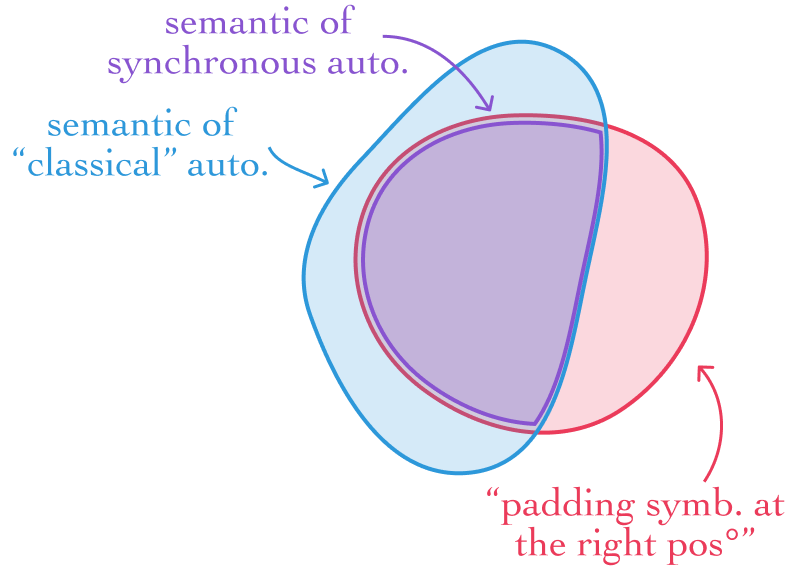
\includegraphics[width=\linewidth]{fig/intro/projection.png}
	\caption{\AP\label{fig:intro-projection}
		Semantics of a "synchronous automaton".
	}
\end{marginfigure}
This approach is ubiquitous in mathematics, and especially in logics:
for instance, first-order logic over "finite structures" is precisely
defined as first-order logic over all "structures", restricted to "finite structures"!
While being natural and ubiquitous, this construction fails to preserve most properties of the logics:
for instance, first-order logic over all "structures" admits a complete proof system,
but does not when restricted to "finite structures". The model-checking problem
is "coRE"-complete over all "structures", but goes to
"RE"-complete---an incomparable complexity class---for "finite structures".
Proving a meta-theorem on such a restriction that explains how some property
behaves in the restricted universe simply by knowing how it behaves on
the larger universe is hence somewhat unexpected but very welcomed!

\begin{contribution}
	We prove that, for any class of "regular languages" satisfying mild closure
	properties, assuming we can decide if a language belongs to this class,
	then we can decide if an "automatic relation" can be written as the restriction
	of a "regular language" in this class to the set of all valid encodings
	of pairs of words.
\end{contribution}

Let us point out that actually, to arrive at this result the notion
of "synchronous algebras" is somewhat intricate. While a more naive definition
exists and makes sense, we show that such a result cannot be proven using this
simpler notion.

This algebraic theory could provide an interesting framework to
study the "$\AUT$/$\REC$-separability problem".
While the class of "recognizable relations" has some desirable
closure properties we need, it lacks others:
unfortunately, it implies that proving the decidability of
the "$\AUT$/$\REC$-separability problem" "via" this framework would
be highly non-trivial.

\begin{openproblemintro}
	Can we decide, given two "automatic relations", if they are "separable@@rel"
	by a "recognizable relation"?
\end{openproblemintro}

In summary, this thesis explores two fundamental perspectives on "homomorphism problems":
the first extends the theory of "conjunctive queries" in database theory by adding regular path
predicates, to capture natural query languages for human-centered graph-shaped data.
It focuses on the problem of query minimization, both in terms of
its total number of atoms, or its tree-width, which is a relevant parameter to
capture the complexity of its evaluation.
The second part focuses on the complexity of problems related to constraint satisfaction
over automatic structures. We show that most \emph{structural} problems, probing the shape of the 
infinite object at hand, are undecidable. In contrast, \emph{language-theoretic} 
problems, dealing with how these infinite structures are represented---or rather how easy it
is to represent them---, remain decidable.


\chapter{Prolegomena}
\label{ch:general-preliminaries}

\begin{chapterpresentation}
	\begin{abstract}
		We introduce the basic definitions and notations used throughout this thesis.
		Rather than reading it linearly, we recommand to skim it
		to get an idea of what it contains, and to only go back to this chapter
		only when needed, using the numerous internal hyperlinks.
	\end{abstract}
		
	\par\bigskip\bigskip
	\chaptertoc
\end{chapterpresentation}

\paragraph*{Notations.}
We try to use notations that syntactically reflect their type:
for instance, given a set $X$, we use Roman lowercases ($x,y,z,\dotsc$)
to denote elements of $X$, Roman uppercases for its subsets ($A, B, C, \dotsc$),
and cursive letters ($\+X, \dotsc$) for sets of subsets of $X$.
Functions are denoted by $f, g, h$, etc. and relations by
uppercase cursive letters ($\+R, \+S, \dotsc$).

Tuples $\tup{x_1,\dotsc,x_k}$ are sometimes denoted by $\bar x$.
Machines (Turing machines, automata, etc.) are also denoted
with uppercase cursive letters ($\+T$, $\+A$, $\dotsc$).
On the other hand, Greek letters are used to either denote queries ($\gamma, \delta, \dotsc$),
formulas ($\phi, \chi, \psi, \dotsc$) or monoid morphisms ($\phi, \chi, \psi, \eta$). When possible, we try to
use the letter to recall the semantics of the object: for instance in
\Cref{ch:semantic-tree-width-CRPQ}, $\gamma$ will be used to denote a base query,
$\alpha$ for one of its "\textbf{a}pproximation@approximation",
$\rho$ for a "\textbf{r}efinements@refinement" and
$\chi$ for an "e\textbf{x}pansion@expansion".
We reserve boldface letters for `complex objects' ("eg"
a "relational structure" $\?A$ or a monad $\?S$), and blackboard bold
for canonical objects ("eg" the natural numbers $\N$) or "pseudovarieties@pseudovariety of monoids".

We will use $\symbb{A}, \symbb{B}, \dotsc$ to denote
alphabets in \Cref{part:databases} and $\Sigma, \Gamma, \dotsc$
to denote them in \Cref{part:automatic}.%
\footnote{Pobody's nerfect…}
Lastly, decision problems are typesetted in small caps
("eg" "finite regular colourability@@pb"), 
complexity classes and categories in sans-serif ("coNP", "ExpSpace", $\Set[]$,
$\Pos[]$).


\section{Set and Functions}

We denote by $\N$, $\Np$ and $\Z$ the sets of natural numbers---that naturally contains zero---,
of strictly positive natural numbers, and of integers, respectively.
For any $n\in\Np$, \AP$\intro*\ZnZ{k}$ denotes the set of integers modulo $k$,
and for any $i,j \in \Z$, $\intro*\intInt{i,j}$ is the set of integers from $i$ to $j$,
bounds included.

The powerset---"ie" the set of all subsets---of a set $X$
is denoted by $\intro*\pset{X}$, and $\intro*\psetp{X}$ is defined analogously
except that subsets are required to be non-empty.
The disjoint union of two sets is denoted by $\sqcup$.

While a function $f$ from set $X$ to set $Y$ is denoted by $f\colon X \to Y$,
we reserve $\intro*\pto$ and $\intro*\surj$ for partial functions and surjections, respectively.
The restriction of a function $f$ to a subset $A$ of its domain is denoted by
$\intro*\restr{f}{A}$, and the identity function $x \mapsto x$ over a set $X$
is denoted by $\intro*\id[X]$.
The domain of a function, be it either total or partial, is denoted
by \AP$\intro*\dom(f)$.
Given a function $f\colon X \to Y$ and a subset $A \subseteq X$,
we denote by $f[A]$ the direct image of $A$ by $f$.%
\footnote{In the literature, $f[A]$ is often abusively denoted by $f(A)$, although
this gives rise to an ambiguity between function application and direct images,
when there exists an element $A \in X$ "st" $A \subseteq X$: this happens for instance
when dealing with von Neumann's ordinals.}
Similarly, given a subset $B \subseteq Y$, $f^{-1}[B]$ denotes
the inverse image of $B$ by $f$, and when $B$ is a singleton $\{b\}$,
we will write $f^{-1}[b]$ instead.%

A binary relation $\+R$ over sets $X$ and $Y$---"ie" a subset $\+R \subseteq X \times Y$---
is said to be \AP""functional@@rel"" when for every $x$, there exists at most one $y$
"st" $\tup{x,y} \in \+R$.
When moreover $X = Y$, we say that it is:
\begin{itemize}
	\itemAP ""reflexive@@rel"" when $\tup{x,x} \in \+R$ for all $x$;
	\itemAP ""symmetric@@rel"" when $\tup{x,y} \in \+R$ "iff" $\tup{y,x} \in \+R$
		for all $x,y$;
	\itemAP transitive when $\tup{x,y} \in \+R$ and $\tup{y,z} \in \+R$
		imply $\tup{x,z} \in \+R$
		for all $x,y,z$.
\end{itemize}
An equivalence relation over $X$ is any binary relation satisfying the three previous axioms.
Given an equivalence class $\sim$ over a set $X$ and an element $x \in X$,
we denote by $\intro*\equivclass[\sim]{x}$ the equivalence class of $x$ under $\sim$.
Lastly, $\defeq$ denotes the definition symbol: $x \defeq y$ means that $x$ is defined as $y$.

\section{Relational Structures}

\subsection{Basic Notions on Structures}

"Relational structures" generalize the concept of "graphs@@dir"
by allowing (1) multiple kinds of relations and
(2) relations of higher arity. This data is made explicit in
the "signature"---also called \emph{vocabulary} or even \emph{schema}.
We start by defining a \AP""purely relational signature"", which consists
in a set of elements, called ""predicates"",%
\footnote{We do \emph{not} assume this set to be finite.}
together with, for each
of these elements, a strictly positive natural number, called \emph{arity}.
We denote by $\+R_{(k)} \in \sigma$ the fact that "predicate" $\+R$, of arity
$k$, is part of "signature" $\sigma$.
Then, a \AP""relational signature"", or \reintro{signature} for short, consists of a "purely relational 
signature" together with a set of constant symbols.%
\footnote{Usually the notion of "signature" also allows for function symbols beyond
the degenerate case of constants. However all the "signatures" considered in the thesis
will be "relational@@signature", justifying the abuse of terminology.}

Then, given a "signature" $\sigma$, a ""$\sigma$-structure"" $\?A$
consists of:
\begin{itemize}
	\item a set $A$, called \emph{domain},
	\item for each "predicate" $\+R_{(k)} \in \sigma$, a $k$-ary relation
		$\+R(\?A) \subseteq A^k$, and
	\item for each constant $c \in \sigma$, an element $c(\?A) \in A$.
\end{itemize}
We call $\+R(\?A)$ (resp. $c(\?A)$) the \AP""interpretation@@predicate""
of "predicate" $\+R_{(k)}$ (resp. constant $c$) in $\?A$.
By analogy with graphs, elements of the domain are sometimes referred to as
\emph{vertices}. See \Cref{fig:example-structure-homomorphism} for an example
of "$\sigma$-structure".

The \AP""graph signature"" is a "purely relational signature"
consisting of a single binary predicate, either written $\+E$ in prefix notation
or $\atom{}$ in infix notation.
Then, the "$\sigma$-structures" over "this signature@graph signature"
exactly consists of \AP""directed graphs"".

An element of $\+R_{(k)}(\?A)$ is called an \AP""$\+R$-tuple""
of "structure" $\?A$. We also use the terminology \emph{edge} in place
of tuple for binary predicates.
An \reintro{hyperedge} of $\?A$ will designate any of its $\+R$-tuples,
indifferently of the "predicate" $\+R$.

A "$\sigma$-structure" $\?A$ is said to be \AP""finite@@struct"" when its
both its domain and its set of "hyperedges" are finite.
In particular, note that this last condition amounts to asking
that (1) for every "predicate" $\+R_{(k)} \in \sigma$, the relation $\+R_{(k)}(\?A)$ is finite,
and (2) there exists only finitely many "predicates" $\+R_{(k)} \in \sigma$
"st" $\+R_{(k)}(\?A)$ is non-empty.

A \AP""substructure"" of a "$\sigma$-structure" $\?A$ is another
"$\sigma$-structure" $\?A'$ "st":
\begin{itemize}
	\item the domain $A'$ of $\?A'$ is a subset of $A$,
	\item each "interpretation@@predicate" of a "predicate" in $\?A'$ 
		is a subset of its "interpretation@@predicate" in $\?A$, and
	\item every constant of $\?A$ belongs to $A'$, and the interpretation
		of the constants in both structures coincide. 
\end{itemize}
A \AP""proper substructure"" is a "substructure" for which
at least one of the inclusions in the first two points above
is strict: in other words, such a "substructure" should
miss at least one element, or one "hyperedge".
Given a subset $X$ of the domain $A$ of a "$\sigma$-structure" $\?A$,
the \AP""substructure of $\?A$ induced by $X$@induced substructure"" is:
\begin{itemize}
	\item undefined if not all constants of $\?A$ belong to $X$,
	\item otherwise, it is obtained from $\?A$ by restricting
		its domain to $X$, and by intersecting its $k$-ary relations
		with $X^k$.
\end{itemize}

The roles played by constants and "predicates" are obviously not symmetric.
For this reason we will often rather deal with "pointed structures".
Formally, given a "purely relational signature" $\sigma$,
a \AP""pointed $\sigma$-structures"" consists of a "$\sigma$-structure"
together with a \emph{tuple} of elements of its domain.
Note that "pointed $\sigma$-structures" with tuples of size $k\in \N$ are in natural
bijection with the set of "$\sigma'$-structures", where $\sigma'$
is obtained from $\sigma$ by adding a set of $k$ constants.

\subsection{Constructions on Structures}

The \AP""disjoint union"" of two "structures" over a
"purely relational signature" 
is obtained by taking the disjoint union of their domain and of
their "predicate interpretations", and is denoted by \AP$\intro*\disunion$.
Over other "signatures", we same apply construction but then identify the constants
in both structures.%
\footnote{Hence this union is not entirely disjoint, however we keep the name
for uniformity. As we will see in \Cref{sec:prelim-db-poset-cq}, this construction
actually satisfies the universal property of co-products.}

\begin{marginfigure}
	\centering
	\begin{tikzpicture}
		\input{tikz/general-prelim/product-cartesian.tex}
	\end{tikzpicture}
	\caption{
		\AP\label{fig:general-prelim-product-Cartesian}
		Two "graphs@@dir" (above and left) and their "Cartesian product" (below right).
	}
\end{marginfigure}
\begin{marginfigure}
	\centering
	\begin{tikzpicture}
		\node[vertex] (x0) at (0,1) {};
\node[vertex] (x1) at (1,1) {};
\node[vertex] (x2) at (2,1) {};
\node[vertex] (y0) at (-1,0) {};
\node[vertex] (y1) at (-1,-1) {};

\foreach \x in {0,1,2} {
	\foreach \y in {0,1} {
		\node[vertex] (\x-\y) at (\x,-\y) {};
	}
}

\draw[edge] (x0) to (x1);
\draw[edge] (x1) to (x2);
\draw[edge] (y0) to (y1);

\foreach \x in {0,1,2} {
	\draw[edge] (\x-0) to (\x-1);
}
\foreach \y in {0,1} {
	\draw[edge] (0-\y) to (1-\y);
	\draw[edge] (1-\y) to (2-\y);
}
	\end{tikzpicture}
	\caption{
		\AP\label{fig:general-prelim-product-block}
		Two "graphs@@dir" (above and left) and their "block product" (below right).
	}
\end{marginfigure}
Let again $\sigma$ to be any "signature".
Given two "$\sigma$-structures" $\?A$ and $\?B$, their
""Cartesian product"" \AP$\?A \intro*\prodstruct \?B$
is defined by taking the Cartesian product of their domain, of
their "predicate interpretations" and of their interpretations of constants. 
Their ""block product"" has the same domain and constants,
but now the "interpretation@@predicate" of "predicate" $\+R_{(k)}$
in the "block product" consists of all tuples
\[\tup{\tup{a_1,b_1}, \dotsc, \tup{a_k,b_k}} \quad\text{"st"}\] 
\begin{itemize}
	\item either $\tup{a_1, \dotsc, a_k} \in \+R(\?A)$ and $b_1 = \dotsc = b_k$, or
	\item $a_1 = \dotsc = a_k$ and $\tup{b_1, \dotsc, b_k} \in \+R(\?B)$.
\end{itemize} 
See \Cref{fig:general-prelim-product-Cartesian,fig:general-prelim-product-block} for examples.
The $k$-fold iteration of $\?A$ is denoted by
$\intro*\iterstruct{\?A}{k}$ and is defined as
\[
	\underbrace{\?A \prodstruct \dotsc \prodstruct \?A}_{k \text{ times}}.
\]
Note that by construction, the "disjoint union", "Cartesian product" and "block product"
of two "structures" over a "signature" yields a "structure" over the \emph{same} "signature".%
\footnote{This is what motivated the somewhat strange definition
of "disjoint union" for "structures" over "signatures" that are not "purely relational@@signature".}

\subsection{Adjacencies}

Given a "$\sigma$-structure" $\?A$ and $a \in A$, we define the \AP""adjacency""%
\footnote{We do not use the terminology \emph{neighbourhood} since it usually refers
to a set of elements, namely the set of elements occurring in the "adjacency".}
of $a$ in $\?A$ to be the tuple of sets%
\AP\phantomintro{\adjacency}
\begin{align*}
	\reintro*\adjacency{a}{\?A}{\+R}{i} & \defeq
	% \Big\langle
		\big\{
			\langle a_1, \dotsc, a_{i-1}, a_{i+1}, \dotsc, a_k \rangle \in A^{k-1}
			\\ & \hphantom{\defeq \big\{ }\mid
			\langle a_1, \dotsc, a_{i-1}, a, a_{i+1}, \dotsc, a_k \rangle \in \+R(\?A)
		\big\},
		% \;\big\vert\;
		% \+R_{(k)} \in \sigma \text{ and } i \in \intInt{1,k}
	% \Big\rangle.
\end{align*}
when $\+R$ ranges over "predicate" of arity $k$ of $\sigma$ and $i \in \intInt{1,k}$. 
For "graphs@@dir", the "adjacency" of a vertex corresponds to its set of predecessors and
its set of successors.

\subsection{Undirected Paths}

An \AP""undirected path"" in a "$\sigma$-structure" $\?A$ consists of a sequence
\[\big\langle a_0,\, \bar h_0,\, a_1,\, \dotsc,\, \bar h_{n-1},\, a_n\big\rangle, \text{ with } n \in \N,\]
where $a_i \in A$ and each $\bar h_i$ is a "hyperedge" of $\?A$ "st" both
$a_i$ and $a_{i+1}$ occur in $\bar h_i$. When such an "undirected path" exists, we say that
there is an "undirected path" between $a_0$ and $a_n$, or equivalently
that $a_0$ and $a_n$ are \AP""connected"".%
\sidenote{Note that this defines an equivalence relation.}
A \AP"connected component" of $\?A$ consists of an equivalence class under this relation.

An ""undirected graph"" consists of a domain, together with
a set of (unordered) pairs of elements of the domain.
The ""incidence graph"" of a "$\sigma$-structure",
for some "signature" $\sigma$, is the following "undirected graph":
\begin{itemize}
	\item its domain is the disjoint union of $A$
		and the "hyperedges" of $\?A$;
	\item there is an edge between two vertices "iff" one of them
		is a vertex $a$ of $\?A$, and the other is an hyperedge
		$\bar h$ of $\?A$, with the property that $a \in \bar h$.
\end{itemize}

The \AP""distance@@struct"" between two vertices of a "$\sigma$-structure"
is defined as half of their distance in the "incidence graph".%
\footnote{By construction the "incidence graph" is bipartite and hence
the distance between two vertices of the "structure" is even.}
The \AP""diameter"" of a "structure" is the maximum over $u$
of the minimum over $v$ of the "distance@@struct" between vertices $u$ and $v$.

The ball \AP$\intro*\ball{\?A}{a}{m}$ centred at vertex $a\in A$ and of radium $r\in\N$ of
a "$\sigma$-structure" $\?A$ is the "substructure" of $\?A$ induced by
all vertices at "distance@@struct" at most $r$.
A "structure" is said to be \AP""locally finite@@structure""
when every ball of finite radius is "finite@@struct".

A \AP""simple path"" in a "$\sigma$-structure" is a
simple path in its "incidence graph"---in other words, 
such a path should alternate between vertices and hyperedges,
and visit each of them at most once.

\subsection{Graphs}

A \AP""directed cycle"" in a "graph@@dir" consists
of a non-empty directed path from a vertex to itself.
A ""directed acyclic graph"", or \reintro{DAG} for short,
is any "graph@@dir" that contains no "directed cycle".

\begin{marginfigure}
	\centering
	\begin{tikzpicture}
		\node[vertex] (n) at (0,0) {};
\node[vertex, below left=of n] (n0) {};
\node[vertex, below right=of n] (n1) {};
\node[vertex, below left=of n1] (n10) {};
\node[vertex, below=of n1] (n11) {};
\node[vertex, below right=of n1] (n12) {};

\draw[edge] (n) to (n0);
\draw[edge] (n) to (n1);
\draw[edge] (n1) to (n10);
\draw[edge] (n1) to (n11);
\draw[edge] (n1) to (n12);
	\end{tikzpicture}
	\caption{\AP \label{fig:general-prelim-directed-tree} A "directed tree".}
\end{marginfigure}
A ""directed tree"" is a non-empty "graph@@dir" "st" there exists 
a vertex $r$ with the property that for every vertex $v$,
there exists exactly one directed path from $r$ to $v$:
see \Cref{fig:general-prelim-directed-tree}.

The ""chromatic number"" of a "graph@@dir" is the least cardinal $k$
"st" it is "$k$-colourable". We say that a "graph@@dir"
is \AP""finitely colourable"" when its "chromatic number" is finite.


\subsection{Homomorphisms}

A \AP""homomorphism"" from a "$\sigma$-structure" $\?A$ to
to a "$\sigma$-structure" $\?B$ consists of a function $f$ from $A$ to $B$,
"st" for every $\+R_{(k)} \in \sigma$, for every $\tup{a_1,\dotsc,a_k} \in \+R(\?A)$,
we have $\tup{f(a_1), \dotsc, f(a_k)} \in \+R(\?B)$. Moreover, for every
constant $c \in \sigma$, we must have $f(c(\?A)) = c(\?B)$.

An \AP""embedding"" is an injective "homomorphism",
whereas a \AP""strong onto homomorphism"" is a "homomorphism" that is both
surjective on the domain and on the "hyperedges". 
The existence of a "strong onto homomorphism" from a "structure" $\?A$
to a "structure" $\?B$ is denoted by \AP$\?A \intro*\surjto \?B$,
and we say that $\?B$ is a \AP""homomorphic image"" of $\?A$.

An \AP""isomorphism"" from $\?A$ to $\?B$ is a "homomorphism" $f\colon \?A \to \?B$
"st" there exists another homomorphism $g\colon \?B \to \?A$ with the property
that $g \circ f = \id[A]$ and $f \circ g = \id[B]$. Equivalently,
it is a "strong onto homomorphism" that is also an "embedding".
Two structures are \AP""isomorphic"", denoted by $\intro*\isom$, if there is an "isomorphism" between them,
and an ""automorphism"" is an "isomorphism" from a "structure" to itself.

\begin{marginfigure}
	\centering
	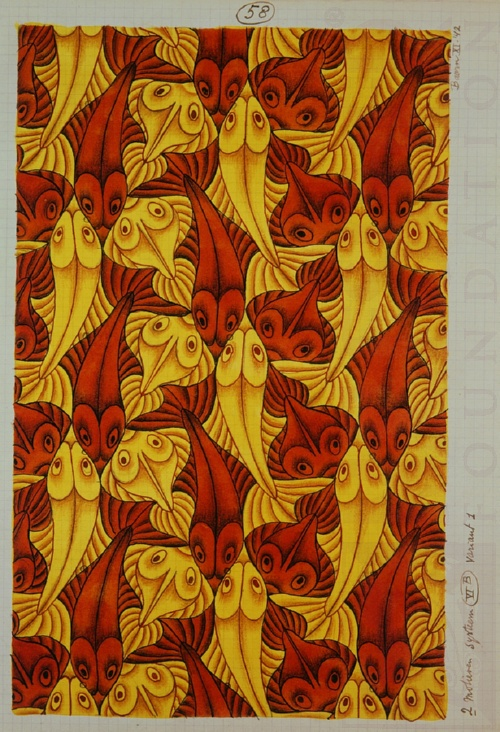
\includegraphics[width=\linewidth]{fig/escher/2-motifs-system.jpg}
	\caption{\href{https://mcescher.com/gallery/symmetry/\#iLightbox[gallery\_image_1]/44}{\emph{2 motifs system VI(b) variant 1}}, M. C. Escher, \textcopyright~The M.C. Escher Company.}
\end{marginfigure}
Given "structures" $\?A_1, \dotsc, \?A_k$ sharing the same "signature",
the $i$-th projection from the Cartesian product $\?A_1 \prodstruct \dotsc \prodstruct \?A_k$
to $\?A_i$, defined by $\tup{a_1,\dotsc,a_k} \mapsto a_i$ ($i \in \intInt{1,k}$),
is a "homomorphism", and is denoted by \AP$\intro*\projHom{i}$.

Given a "$\sigma$-structure" $\?A$, a \AP""congruence@@struct"" on $\?A$
is an equivalence class $\sim$ of $A$ "st" for every
$\+R_{(k)} \in \sigma$, for every $\tup{a_1,\dotsc,a_k} \in \+R(\?A)$,
for any tuple $\tup{a'_1,\dotsc,a'_k} \in A^k$ "st" $a_i \sim a'_i$ for each $i\in \intInt{1,k}$,
then $\tup{a'_1,\dotsc,a'_k} \in \+R(\?A)$.
The \AP""quotient structure"" defined by a "congruence@@struct" $\sim$
on a "structure" $\?A$ has the equivalence classes of $\sim$ as its domain,
and natural "interpretation@@predicates" of the "predicates" and constants.

Given a "homomorphism" $f\colon \?A \to \?B$,
the \AP""congruence induced"" by $f$, and denoted by $\intro*\ker{f}$
is defined by $a \ker{f} a'$ "iff" $f(a) = f(a')$ for all $a, a' \in A$.
It is routine to check that it is indeed a "congruence@@struct" on $\?A$.

We will often implicitly use Noether's first isomorphism theorem:
the "substructure" of $\?B$ "induced@@substructure" by the image $f[A]$
of $A$ is "isomorphic" to the "quotient@@struct" of $\?A$ by $\ker{f}$.

\subsection{Cores}

Two "$\sigma$-structures" $\?A$ and $\?B$ are ""homomorphically equivalent""
if $\?A \homto \?B$ and $\?B \homto \?A$.

A retraction of $\?A$ is a "substructure" $\?A'$ of $\?A$ together with
a "homomorphism" from $\?A$ to $\?A'$ with the property that any vertex of $A'$
is sent on itself.
\begin{proposition}
	Any "finite $\sigma$-structure" $\?A$ admits a unique minimal (in the number of vertices) retraction.
\end{proposition}

\begin{figure}
	\centering
	\begin{tikzpicture}
		\node[vertex, draw=c1, fill=c1, fill opacity=.4] at (0,1) (a) {};
		\node[vertex, draw=c0, fill=c0, fill opacity=.4] at (1.414,1) (b) {};
		\node[vertex, draw=c2, fill=c2, fill opacity=.4] at (2.828,1) (c) {};
		\node[vertex, draw=c1, fill=c1, fill opacity=.4] at (4.242,1) (d) {};
		\node[vertex, draw=c2, fill=c2, fill opacity=.4] at (0.707,0) (e) {};
		\node[vertex, draw=c1, fill=c1, fill opacity=.4] at (2.121,0) (f) {};
		\node[vertex, draw=c3, fill=c3, fill opacity=.4] at (3.536,0) (g) {};
		\node[vertex, draw=c0, fill=c0, fill opacity=.4] at (4.950,0) (h) {};

		\draw[edge] (a) to (b);
		\draw[edge] (b) to (e);
		\draw[edge] (f) to (b);
		\draw[edge] (b) to (c);
		\draw[edge] (f) to (c);
		\draw[edge] (g) to (f);
		\draw[edge] (c) to (g);
		\draw[edge] (d) to (c);
		\draw[edge] (g) to (d);
		\draw[edge] (d) to (h);

		\begin{scope}[xshift=5.5cm]
			\node[vertex, draw=c0, fill=c0, fill opacity=.4] at (1.414,1) (b2) {};
			\node[vertex, draw=c2, fill=c2, fill opacity=.4] at (2.828,1) (c2) {};
			\node[vertex, draw=c1, fill=c1, fill opacity=.4] at (2.121,0) (f2) {};
			\node[vertex, draw=c3, fill=c3, fill opacity=.4] at (3.536,0) (g2) {};

			\draw[edge] (f2) to (b2);
			\draw[edge] (b2) to (c2);
			\draw[edge] (f2) to (c2);
			\draw[edge] (g2) to (f2);
			\draw[edge] (c2) to (g2);
		\end{scope}
	\end{tikzpicture}
	\caption{
		\AP\label{fig:prelim-core}
		On the left-hand side a "graph@@dir", and its "core" on the right.
		The colours are not part of the "structure", but
		are used to describe the retraction of the original
		structure onto its "core".
		(Replica of \Cref{fig:intro-core}.)
	}
\end{figure}
\begin{proof}
	The existence is trivial.
	For the uniqueness, consider two retractions $f_1\colon \?A \homto \?B_1$
	and $f_2\colon \?A \homto \?B_2$. We want to prove that $\?B_1$ and $\?B_2$ are
	"isomorphic".
	Since $\?B_1$ is a "substructure" of $\?A$, consider
	$\restr{f_2}{B_1}\colon \?B_1 \homto \?B_2$. By minimality of $\?B_2$, this "homomorphism"
	must be surjective.
	By symmetry, $\restr{f_1}{B_2}\colon \?B_2 \homto \?B_1$ is also a surjective "homomorphism".
	By composition, we obtain surjective "homomorphism" from $\?B_1$ to itself and from $\?B_2$ to itself. By finiteness, these surjective "homomorphisms" must actually be "automorphisms".
	Hence, it follows that $\restr{f_2}{B_1}$ and $\restr{f_1}{B_2}$ are "isomorphisms",
	and hence $\?B_1$ is "isomorphic" to~$\?B_2$.
\end{proof}

This unique minimal retraction of $\?A$ is called \AP""core"" of $\?A$ and
is denoted by \AP$\intro*\core{\?B}$.
By construction, the "core" of $\?A$ is a "substructure" of $\?A$ to which it is "homomorphically equivalent", see \Cref{fig:prelim-core}.
In general, a \reintro{core} is any "$\sigma$-structure" such that is the "core" of
some "structure"---or equivalently of itself.

\begin{proposition}
	\AP\label{prop:core-iff-hom-are-auto}
	A "finite $\sigma$-structure" $\?C$ is a "core" if, and only if, every
	homomorphism from $\?C$ to itself is an "automorphism".
\end{proposition}

\begin{proof}
	For the left-to-right implication,
	we let $f\colon \?C \to \?C$ be a "homomorphism".
	Then $f[\?C]$ must be "isomorphic" to $\?C$, otherwise we would obtain
	a strictly smaller retraction. Hence, $f$ is a "strong onto homomorphism"
	from $\?C$ to itself, and hence is an "automorphism".
	
	Conversely, assuming that any "homomorphism" from $\?C$ to itself is an "automorphism"
	we get in particular that any retraction must be an "automorphism", and
	hence that $\?C$ is "isomorphic" to $\core{\?C}$.
\end{proof}

\begin{proposition}
	\AP\label{prop:equiv-core-isomorphic}
	Two "finite structures" are "homomorphically equivalent" if,
	and only if, their "core" are "isomorphic".
\end{proposition}

\begin{proof}
	The right-to-left implication is trivial.
	For the converse one, denote the two "structures" by $\?A_1$ and $\?A_2$,
	and suppose that $\?A_1$ is "homomorphically equivalent" to $\?A_2$.
	Using the "homomorphical equivalence" of $\?A_1$ and $\?A_2$,
	we get retractions of $\?A_2$ onto $\core{\?A}_1$ and of $\?A_1$ onto $\core{\?A}_2$.
	It follows that we have surjective "homomorphisms" from $\core{\?A}_1$ to $\core{\?A}_2$
	and conversely. Hence, $\core{\?A}_1$ and $\core{\?A}_2$ are "isomorphic".
\end{proof}

\begin{proposition}
	\AP\label{prop:adjacency-core}
	Given a "$\sigma$-structure" $\?B$, if $\?B$ is a "core", then
	two elements $b_1$ and $b_2$ of $\?B$ have the same "adjacency" "iff" $b_1 = b_2$.
\end{proposition}

\begin{proof}
	The right-to-left implication is trivial.
	For the converse one, consider the "homomorphism" from $\?B$ to itself
	which maps $b_2$ to $b_1$, and all elements of $B \smallsetminus \{b_2\}$
	to themselves. Since we assumed that $b_1$ and $b_2$ have the same "adjacency",
	this is indeed a "homomorphism", which is clearly not bijective, and
	$\?B$ is not a "core".
\end{proof}

\section{Logic Related Notions}

\subsection{First-Order Logic and Beyond}
\label{sec:prelim-fo}

We fix a "purely relational signature" $\sigma$.
A (semantical) Boolean \AP""query@@sem"" is any subclass of the
class of all "$\sigma$-structures".
More generally, a $k$-ary \reintro(sem){query} is a function
that maps any "$\sigma$-structure" to a (potentially empty) set of $k$-tuples
of vertices.
We now turn to more syntactical definitions of queries.

We assume that we are given a countable infinite set of variables.
A \AP""first-order formula"" is any formula generated by the grammar 
\[
	\phi \mathrel{{:}{:}{=}} \+R(x_1,\dotsc,x_k) \mid \neg \phi \mid \phi \lor \phi \mid \phi \land \phi
	\mid \exists x.\, \phi \mid \forall x.\, \phi,
\]
where the $x_i$'s ranges over the set of variables and $\+R_{(k)}$ over the "signature" $\sigma$.

\begin{hypothesis}
We assume that, even when not mentioned explicitly, the "signature" contains
a binary "predicate" $=$ that is "interpreted@@predicate" over all "structures"
as equality.
\end{hypothesis}

A \AP""first-order sentence"" is any "first-order formula" with no free variable.
Given a "first-order formula" $\phi$ with free variables $\bar x$, denoted by $\phi(\bar x)$,
and a "pointed $\sigma$-structure" $\tup{\?A,\bar a}$ where the arity of $\bar a$ coincide with
the one of $\bar x$, we denote by $\tup{\?A,\bar a} \intro*\FOmodels \phi(\bar x)$
the fact that $\tup{\?A,\bar a}$ is a model of $\phi(\bar x)$: this can be defined by
a trivial induction on the formula, by interpreting:
\begin{itemize}
	\item the free variable $x_i$ as $a_i$,
	\item the "predicates" $\+R$ as the relation $\+R(\?A)$,
	\item $\neg$, $\lor$, $\land$, $\exists$ and $\forall$ as the Boolean operators of negation, disjunction and conjunction, and as the existential and universal quantifiers, respectively.
\end{itemize}
Given a "$\sigma$-structure" $\?A$, we then denote by \AP$\intro*\semFO{\phi(\bar x)}{\?A}$
the set of tuples $\bar a$ "st" $\tup{\?A, \bar a} \FOmodels \phi(\bar x)$.

\begin{remark}
	\label{rk:prelim-formula-tuple}
	For technical reasons---that will be explained in \todo{ref}---,
	we allow variable repetition in $\bar x$. The only constraint on $\bar x$
	is that the set of variables occurring in $\bar x$ 
	should exactly be the set of free variables of $\bar x$.
	Strictly speaking, the data $\phi(\bar x)$ is richer than just a
	formula, however we will abusively still this pair \emph{formula}.
\end{remark}

We now define the classes $\Pi_n$ and $\Sigma_n$ ($n\in\N$) of "first-order formulas"
as least fixpoints, with the property that $\Sigma_0 \subseteq \Sigma_1 \subseteq \dotsc$ and dually for $\Pi_n$.
We let $\Sigma_0 = \Pi_0$ be the set of quantifier-free formulas.
Then for all $n\in\N$, we consider the following rules:
\[
	\frac{
		\phi \in \Sigma_n
	}{
		\neg \phi \in \Pi_n
	} \qquad\text{and}\qquad
	\frac{
		\phi \in \Pi_n
	}{
		\neg \phi \in \Sigma_n
	},
\]
moreover $\Pi_n \subseteq \Sigma_{n+1}$ and $\Sigma_{n+1}$ is closed under
disjunction, conjunction and existential quantification,
and dually $\Sigma_n \subseteq \Pi_{n+1}$ and $\Pi_{n+1}$ is closed under
disjunction, conjunction and universal quantification.
Formally, the hierarchies
\[
	\Sigma_0 \subseteq \Sigma_1 \subseteq \cdots
	\qquad\text{and}\qquad
	\Pi_0 \subseteq \Pi_1 \subseteq \cdots
\]
are defined as the smallest sets of formulas satisfying these rules.
Then, the \AP""quantifier alternation rank"" of a formula $\phi(\bar x)$
is the least $n\in\N$ "st" $\phi(\bar x)$ belongs to either
$\Sigma_n$ or $\Pi_n$.
Formulas from $\Sigma_1$ are called ""existential formulas"",
those that neither contain negations nor universal quantifications are called \AP""existential-positive formulas"" and lastly, those that neither contain negations
nor any quantifier
are called ""positive quantifier-free formulas"".

A relation over a "$\sigma$-structure" $\?A$ is said to be
\AP""first-order definable"" when it can be written as
$\semFO{\phi(\bar x)}{\?A}$ for some "first-order formula" $\phi(\bar x)$.
Moreover, a class of "$\sigma$-structures" is said to be \reintro{first-order definable},
when there exists a "first-order sentence" $\phi$ "st" the class of "structures" $\?A$
"st" $\?A \FOmodels \phi$ is precisely the class itself.

\AP""First-order logic"" simply consists of the syntax of "first-order formulas" together
with their semantics. Lastly, \AP""monadic second-order logic""
(resp. ""second-order logic"") is obtained from "first-order logic"
by also allowing quantifications over subsets of the structure
(resp. relations of arbitrary arity over the structure).

\subsection{Automata Theory}

Given a set $X$, we denote by $X^*$ and $X^+$ the set of finite words
over $X$, and of non-empty finite words over $X$, respectively.
The empty word is denoted by $\varepsilon$.
An \emph{alphabet} is nothing else but a finite set, and we denote by
$\intro*\2$ the binary alphabet $\{0,1\}$.

In an automaton $\+A$, we denote by \AP $p \intro*\transition{a} q \in \+A$
the fact that there is an $a$-labelled transition from $p$ to $q$.
A \AP""regular language"" is any language---"ie" subset of $\Sigma^*$ for some alphabet $\Sigma$---that
can be recognized by a finite-state automaton.

The signature of words over $\Sigma$ has a binary "predicate" $\preceq$
as well as a unary predicate $a$ for each $a\in \Sigma$.
A word $w_0 \cdots w_{n-1}$ of length $n$
can be seen as a "structure" over the signature of $\Sigma$-words
by taking $\intInt{0,n-1}$ as its domain, "interpreting@@predicate"
$\preceq$ naturally, and interpreting $a\in \Sigma$
as the set of $i \in \intInt{0,n-1}$ "st" $w_i = a$.
It is well-known%
\footnote{See \Cref{sec:preliminaries-automatic-structures-relations-landscape} for details.}
that a language is "regular@@lang" if, and only if, it is definable in "monadic second-order logic".
When $\Sigma = \2$, the signature of $\Sigma$-words is also called 
the \AP""signature of binary strings"".

\subsection{Monoids}

We refer the reader to Pin's seminal lecture notes \cite{Pin2022MathematicalFoundations}
for an introduction to algebraic language theory.

A \AP""monoid"" $\?M = \tup{M,{\cdot},1}$ is a set $M$ together with an associative binary operator $\cdot$ called \emph{product}, and an element $1 \in M$, called \emph{unit}, "st" $x\cdot 1 = x = 1 \cdot x$ for all $x\in M$.
%An \AP""idempotent"" is any element $x\in M$ "st" $x = x^2$.
A \AP""monoid morphism"" is a function between monoids that preserve the product and unit.

"Monoids"---or rather "monoid morphisms"---can be used to recognize languages as $\Sigma^*$
is itself a monoid under concatenation---actually, it is \emph{the free monoid} over $\Sigma$.
A language $L$ is "regular@@lang" if, and only if, there exists a "finite monoid" $\?M$,
and subset $\Acc \subseteq M$ (called \emph{accepting elements}), and a "monoid morphism"
$\phi\colon \Sigma^* \to M$ "st" $L = \phi^{-1}[\Acc]$.
Another way of thinking of the pair $\tup{\phi, M}$ is as follows:
a deterministic complete semiautomaton can be described as a set $Q$ together
with a monoid right action of $\Sigma^*$ over $Q$. On the other hand,
a surjective monoid morphism $\phi\colon \Sigma^* \surj M$ consists of both a monoid
left action and a monoid right action of $\Sigma^*$ over a set $M$,
with the property that $u \cdot (x \cdot v) = (u \cdot x) \cdot v$ for all 
$x\in M$ and $u,v \in \Sigma^*$.
In other words, while automata states represent some information on the word
that is updatable by appending letters on the right, monoid elements represent
an information on the word that is updatable both by appending letters on the left or the right. 

Unsurprisingly, there is a notion of ``minimal information'' required to recognize a monoid,
giving rise to the notions of ""syntactic monoids"" and ""syntactic morphisms"",
see "eg" \cite[Theorem~1.7]{Bojanczyk2020MSO}.

Submonoids and quotient structures are defined analogously to
"substructures" and "quotient structures" for "relational structures".
We say that a "monoid" \AP""divides@@monoid"" another one if it is
a submonoid of one of its quotients.
A \AP""pseudovariety of monoids"" $\symbb{V}$%
consists in a set of "finite monoids" closed under finite Cartesian products
and "monoid division".%
\footnote{``Pseudovariety of \emph{foo}'' and ``variety of finite \emph{foo}''
are used interchangeably in the literature.}
For more details on these,
see \cite[\S XI.1, p.~189]{Pin2022MathematicalFoundations} under the name ``variety''.
On the other hand, a ""$\ast$-pseudovariety of regular languages""
consists of \emph{stream}, "ie" a function $\+V\colon \Sigma \mapsto \+V_{\Sigma}$ from alphabets to languages over this alphabet, with the following properties:%
\footnote{See also \cite[\S XIII.3, p.~226]{Pin2022MathematicalFoundations}.}
\begin{itemize}
	\item it is closed under Boolean operators;
	\item it is closed under preimages by "monoid morphisms", in the sense that
		for every monoid morphism $\phi\colon \Gamma^* \to \Sigma^*$, for any $L \in \+V_{\Sigma}$,
		then $\phi^{—1}[L] \in \+V_{\Gamma}$, and
	\item it is closed under residuals, in the sense that for any $L \in \+V_{\Sigma}$,
		for any $u\in\Sigma^*$, then
		$u^{-1}L \defeq \{v \in \Sigma^* \mid uv \in L\}$
		and $Lu^{-1} \defeq \{v \in \Sigma^* \mid vu \in L\}$
		both belong to $\+V_{\Sigma}$.
\end{itemize}
A seminal result by Eilenberg shows that, mapping a "pseudovariety of monoids" $\symbb{V}$
to the stream associating to $\Sigma$ the set of languages over $\Sigma$ that are recognized
by a "monoid" from $\symbb{V}$ yields a "$*$-pseudovariety of regular languages",
and moreover, this operation is a bijection!
This result generalizes Schützenberger's infamous theorem, showing that
star-free languages are exactly those recognized by aperiodic monoids:
for this reason, this bijection is called the \AP""Eilenberg-Schützenberger correspondence@@lang"".%
\footnote{See \cite[Theorem XIII.4.10, p.~228]{Pin2022MathematicalFoundations} for more details.}

Lastly, given a stream of regular languages $\+V$, the \AP""$\+V$-membership problem@@lang""
takes as input an alphabet $\Sigma$ and a "regular language" $L \subseteq \Sigma^*$,
and asks if $L \in \+V_{\Sigma}$. When $\+V$ is a "pseudovariety of regular languages",
a powerful technique to solve this problem is to prove that the membership problem
of the "corresponding@@EilenbergLang" "pseudovariety of monoids" is decidable.

\section{Computability and Complexity}

\subsection{Turing Machines}

\marginnote{\blockquote[Gilles Dowek, Laurence Devillers \& Serge Abiteboul, \emph{Qui a hacké Garoutzia}]{Mais dans ce sandwich absurde entre mon initialisation et ma terminaison, que m'aura-t-il vraiment manqué ? Peut-être un corps… un corps qui ressent et tutti quanti !}}
We assume that the reader is familiar with Turing machines,
see "eg" \cite[\S~1]{AroraBarak2009ComputationalComplexity}.
Unless stated otherwise, a \AP""Turing machine"" is assumed to have a single tape,
which is bounded on the left but not on the right.
The ""configuration@@TM"" of a "Turing machine" consists of
the content of the tape at a given point, the position of the machine's head,
at well as its current state. It can be summarized by
a triple $\tup{u, q, v}$, where $q$ denotes the current state,
$u$ is the word written strictly on the left of the head,
and $v$ is the word written to the right of the head (head included).
The \AP""initial configuration"" of a "Turing machine" $\+M$ refers to the "configuration@@TM" 
$\tup{\varepsilon, q_0, \varepsilon}$ where $q_0$ is the initial state of $\+M$.
A "configuration@@TM" is \AP""reachable@@configuration"" whenever
it can be obtained from the "initial configurations" by applying a finite sequence
of transitions of the machine.

\subsection{Elements of Complexity Theory}

We assume familiarity with basic complexity classes, see "eg"
\cite[\S\!\S~2--5]{AroraBarak2009ComputationalComplexity}.
We say that two decision problems are \AP""computationally equivalent""
when there are many-one reductions between them.

% REPLACE NEXT PARAGRAPH WITH: WHEN FIGURE WILL BE DONE.
% In the following hierarchy, we
% describe the different complexity classes that appear in this document:
% those appearing in bold play a `crucial role' in this thesis and are briefly defined
% in this document; the other ones---they are often only mentioned when talking about
% the literature---point to the "Complexity Zoo".
% We also mention a few decisions problems studied in this thesis---they will be introduced
% as needed.

\paragraph*{Complexity Classes.}
Here are the most important classes that appear in this document---the other ones
will all point to their respective entry in the "Complexity Zoo":
\begin{itemize}
	\item "FOfin" refers to "first-order definable classes", see \Cref{sec:prelim-auto-FO} for the definition;
	\itemAP ""L"" and ""NL"" refer to problems solvable in deterministic and non-deterministic logarithmic 
	space; for hardness we usually consider "first-order reductions";
	\itemAP ""P"" (resp. ""PSpace"") refers to problems solvable in deterministic polynomial time
	(resp. polyomial space); hardness is usually considered under logarithmic-space reductions;
	\itemAP ""NP"" and ""coNP"" refer to the first level of the polynomial-time hierarchy
		\cite[\S~2]{AroraBarak2009ComputationalComplexity},
		and ""SigmaP2"", ""PiP2"" to its second level,
		see "eg" \cite[\S~5]{AroraBarak2009ComputationalComplexity};
		hardness is usually considered under logarithmic-space reductions;
	\itemAP ""$k$-ExpTime"" and ""$k$-ExpSpace"" are the
		problems solvable in time and space
		\[n \mapsto \underbrace{2^{2^{{\,\rotatebox{90}{\tiny$\ddots$}\,}^{2^{\poly(n)}}}}}_{k \text{ times}},\]
		respectively; hardness is considered under polynomial-time reductions;
	\itemAP ""Tower"" is the class of problems that can be solved in time
		$n\mapsto \tower(f(n))$ for some elementary function $f$,%
		\footnote{Recall that an function is said to be elementary when it
		is bounded by a tower of exponentials of fixed height.}
		where $\intro*\tower(n) \defeq t(n,n)$ and $t$ is the function
		defined recursively by $t(p,q) \defeq 2^{t(p-1,q)}$ and $t(0,q) \defeq q$:
		in other words $\tower(n)$ it is a tower of exponentials whose height is given by the input;
		hardness is defined under elementary reductions,
		see \cite{Schmitz2016ComplexityHierarchies} for more details on this class.
\end{itemize}

\paragraph*{Computability Classes.}
We now turn to undecidable classes: all hardness result are considered up to
many-one reductions, "ie" instance-preserving computable functions.
We denote by \AP""RE"" and ""coRE"" the classes of recursively enumerable
and co-recursively enumerable problems, respectively. 
The next levels $\Sigma^0_n$ and $\Pi^0_n$ of the \AP""arithmetical hierarchy"" can be defined 
as the classes of sets that are "definable@@first-order" by a "first-order formula"
from the fragments $\Sigma_n$ and $\Pi_n$, respectively, in the structure $\tup{\N,+,\cdot}$.
It can be shown that $\Sigma^0_0 = \Pi^0_0$ corresponds to the class of all decidable problems,
and $\Sigma^0_1 =$ "RE" and $\Pi^0_1$ = "coRE". The only other levels that will be of interest
to us will be \AP""Sigma0-2"" and ""Pi0-2"".
The ""analytical hierarchy"" is defined analogously, by replacing "first-order logic" with
"second-order logic".


\paragraph*{Decision Problems.}
\AP""Connectivity in Finite Graphs"" is the decision problem
that takes as input a "graph@@dir" and two vertices $s$ and $t$,
and asks if they are "connected".
\AP ""Reachability in Finite Graphs"" is defined analogously,
but asks rather if there is a directed path from $s$ to $t$.
Surprisingly, despite their resemblance, these two problems have a distinct complexity:
"Reachability in finite graphs" is "NL"-complete, see "eg"
\cite[Theorem~4.18]{AroraBarak2009ComputationalComplexity}, while "Connectivity in finite graphs"
is only in "L" by Reingold's theorem, see "eg"
\cite[Theorem~21.21]{AroraBarak2009ComputationalComplexity}.
In fact, the problem is "L"-complete:
Etessami even proved that the problem
was "L"-hard under "first-order reductions" even if the "graph@@dir" is restricted to
be a "directed path@$k$-path" \cite[Theorem 3.2]{Etessami1997CountingLogSpace}!

\part{Querying Graph Databases}

\chapter{Query Languages for Graph Databases}
\label{ch:prelim-graph-databases}
\renewcommand\thefigure{\thechapter.\arabic{figure}}

\begin{chapterpresentation}
	\begin{abstract}
		This preliminary chapter briefly surveys the literature on
		the notion of \emph{conjunctive queries},
		\emph{conjunctive regular path queries} and related notions.

		\todo{finish}
	\end{abstract}
	\par\bigskip\bigskip
	\begin{acknowledgements}
		Parts of this chapter come from the introduction and preliminaries of \cite{FigueiraMorvan2025SemanticTreeWidthLMCS,FigueiraMorvanRomero2025Minimizing}.
	\end{acknowledgements}
	\clearpagepresentation
	\chaptertocstandalone
\end{chapterpresentation}

\section{Relational Databases}
\label{sec:prelim-db-relational}

\subsection{SQL and First-Order Logic}

The most common model of databases is by far that of "relational databases",
in which data is stored in \emph{tables}: an example is depicted
in \Cref{fig:relational-database-cinema}.

\begin{table}
	\centering%
	{%
	\footnotesize%
	\begin{tabular}{cccc}
		\multicolumn{4}{c}{\textsc{Movies}} \\ \toprule
		id & title & length & director \\ \midrule
		197 & Eyes Wide Shut & 159 & Stanley Kubrick \\ 
		205 & J'ai tué ma mère & 96 & Xavier Dolan \\
		304 & Amadeus & 161 & Miloš Forman \\
		321 & 120 Battements par minute & 143 & Robin Campillo \\ \bottomrule
	\end{tabular}
	\\\bigskip%
	\begin{tabular}{cc}
		\multicolumn{2}{c}{\textsc{Rooms}} \\ \toprule
		id & capacity  \\ \midrule
		1 & 108 \\
		2 & 124 \\
		3 & 96 \\
		4 & 102 \\ \bottomrule
	\end{tabular}%
	\hspace{1cm}%
	\begin{tabular}{ccc}
		\multicolumn{3}{c}{\textsc{Projections}} \\ \toprule
		movie\_id & room\_id & time \\ \midrule
		197 & 2 & 2025-03-28 14:00 \\
		205 & 3 & 2025-03-28 14:30 \\
		321 & 4 & 2025-03-28 14:30 \\
		197 & 1 & 2025-03-28 17:00 \\ \bottomrule
	\end{tabular}
}
	\caption{
		\AP\label{fig:relational-database-cinema}
		A "relational database" consisting of three tables, representing data
		stored by a cinema. (Replica of \Cref{fig:example-db-as-rel}.)
	}
\end{table}

Formally, a \AP""pointed relational database"" $\tup{\?D, \bar d}$
over a "purely relational signature" $\sigma$
consists of, for each "predicate" $\+R$ of arity $k$ in $\sigma$,
a $k$-ary relation $\+R_{(k)}(\?D)$, as well as a tuple $\bar d$ of elements,
called \emph{constants}.
A \AP""relational database"" is a "pointed relational database" whose tuple is empty.%
\footnote{It is often asked that at least one $\+R_{(k)}(\?D)$ is non-empty.
Whether this condition is imposed does change the theory---for instance the "first-order sentences"
that are valid over all non-empty structures is a strict supset of
those valid over all (possibly empty) structures.
However, this condition is mostly required for historical reasons,
and whether the databases are allowed to be non-empty
will be of little importance for the query languages we will consider.}
A tuple occuring in some relation $\+R_{(k)}(\?D)$ is called a \emph{fact}.
From a practical perspective, relations model the tables,
while each fact corresponds to some row: for 
instance the database of \Cref{fig:relational-database-cinema}
has three relations, twelve facts and no constants.%
\footnote{Many variations on the definition above exists:
for instance the columns of the table are often given a name (called \emph{attribute}),
see "eg" \cite[\S\!\S~3.1--3.2]{AbiteboulHullVianu1995Databases}.
This is usually done to make the syntax of relational algebra easier on the eye,
however this is only syntactic sugar \cite[Proposition~5.1.2]{AbiteboulHullVianu1995Databases}.}

Naturally, each "relational database" yields a "$\sigma$-structure" whose
domain is the set of elements occurring in some fact of the database or as a constant.
This structure has the property that each vertex either belongs to some "hyperedge" or
is a constant: in other words, it has no \AP""isolated vertices"".
This mapping is in fact one-to-one: "relational databases" over $\sigma$
are in bijection with "$\sigma$-structures" with no "isolated vertices".

\begin{hypothesisnotation}
	We identify (pointed) "relational databases" with (pointed) "relational structures"
	with no "isolated vertices".
\end{hypothesisnotation}

As mentioned in \Cref{ch:intro}, from a theoretical perspective,
a very natural way of querying these "structures"
is "via" "first-order logic". Remarkably, it is exactly as expressive 
as the fragment of SQL generated by
\begin{align}
	\phi_{(k)}\; & \mathrel{{:}{:}{=}} \sqlop{SELECT DISTINCT} \textrm{ attribute}_1, \dotsc, \textrm{ attribute}_k\notag\\
	& \hphantom{\mathrel{{:}{:}{=}}} \sqlop{FROM } \phi_{(i_1)}, \dotsc, \phi_{(i_n)}\notag\\
	& \hphantom{\mathrel{{:}{:}{=}}} \sqlop{WHERE} \textrm{ some condition} \label{eq:sql-fo}\\
	& \;\mid \textrm{some table of arity $k$} \notag\\
	& \;\mid \phi_{(k)} \mathrel{\sqlop{ UNION }} \phi_{(k)}
		\mid \phi_{(k)} \mathrel{\sqlop{ EXCEPT }} \phi_{(k)}
		\mid \phi_{(k)} \mathrel{\sqlop{ INTERSECT }} \phi_{(k)}, \notag
\end{align}
where $i_1 + \dotsc + i_n = k$ and the condition after $\sqlop{WHERE}$
is a conjunction of equalities between attributes.
Dealing with the arity $k \in \N$ is required to ensure "eg" that the union 
is homogeneous---"ie" that all facts in the union have the same arity.%
\footnote{Also, the \textsf{DISTINCT} keyword is only necessary because SQL
has a multiset semantics rather than a set-based semantics…}

\begin{proposition}[Codd's theorem {\cite[\S~4]{Codd1972RelationalCompleteness}}]
	\!\footnote{Codd's theorem actually deals
	with \emph{relational algebra} rather than SQL.
	The equivalence between \emph{relational algebra} and the fragment
	\eqref{eq:sql-fo} of SQL is however straightforward.
	See also \cite[Theorem~5.4.6]{AbiteboulHullVianu1995Databases}.}
	\AP\label{prop:codd-thm}
	"First-order logic" over "$\sigma$-structures" with no "isolated vertices"
	is equally expressive to the SQL fragment defined in \eqref{eq:sql-fo}.
	Moreover, this equivalence is effective.
\end{proposition}

\begin{proof}[Proof sketch]
	\emph{Warning:} dealing with all the subtleties of the proof is actually
	somewhat tedious. Hence, we provide an \emph{informal} proof,
	which prioritizes intuition over formalism.

	\proofcase{From SQL to FO.}
	Expressing a SQL query as a "first-order formula" is intuitive,
	by generalizing the idea given in \Cref{sec:intro-cq}:
	\begin{itemize}
		\item $\sqlop{UNION}$, $\sqlop{EXCEPT}$ AND $\sqlop{INTERSECT}$
			are interpreted as the union, set difference ("ie" $- \land (\neg -)$)
			and intersection;
		\item a table of arity $k$, modelled as a relation $\+R_{(k)}$,
			is encoded as the atomic formula
			\[
				\phi_{(k)}(x_1,\hdots,x_k) \defeq \+R_{(k)}(x_1,\hdots,x_k)
			\]
			with $k$ free variables which are all fresh;
		\item a query
			\begin{align*}
				& \sqlop{SELECT DISTINCT} \textrm{ attribute}_1, \dotsc, \textrm{ attribute}_k \\
				& \sqlop{FROM } \phi^1_{(i_1)}, \dotsc, \phi^n_{(i_n)} \\
				& \sqlop{WHERE } \theta 
			\end{align*}
			is encoded as
			\[
				\psi(y_1,\hdots,y_k) \defeq
				\exists \bar x.\;
				\phi^1_{(i_1)}(x^1_1,\dotsc,x^1_{i_1})
				\land \dotsc \land
				\phi^n_{(i_n)}(x^n_1,\dotsc,x^n_{i_n})
				\land \theta,
			\]
			with $y_1$, $\dotsc$, $y_k$ being the variable associated
			to the attributes---"eg" if $\textrm{attribute}_1$ is the
			third attribute of $\phi^2$, then $y_1 \defeq x^2_3$---
			and $\bar x$ is the tuple of all variables of the form $x^i_j$
			that are distinct from the $y_i$'s.
	\end{itemize}
	
	\proofcase{From FO to SQL.}
	The converse encoding, "ie" from first-order logic to SQL queries,
	is a little more tricky:
	\begin{itemize}
		\item union is encoded with \sqlop{UNION},
			intersection and existential quantification with
			\sqlop{SELECT DISTINCT}-\sqlop{FROM}-\sqlop{WHERE};
		\item we encode negation using \sqlop{EXCEPT} and a SQL query
			that outputs every $k$-tuple of vertices of the "structure"---this query can
			be written as a big union of \sqlop{SELECT DISTINCT}-\sqlop{FROM}
			queries;
		\item lastly, universal quantification can then be obtained
			using the tautology
			\[\forall x.\; \phi(x) \equiv \neg\exists x.\; \neg \phi(x).\qedhere\]
	\end{itemize}
\end{proof}

A crucial ingredient that ensures the correctness of these encodings
is actually the fact that "relational databases" are encoded
as "relational structures" \emph{with no "isolated variables"}.%
\footnote{The restriction of "first-order logic" to
"relational databases" is usually called \emph{relational calculus}.}
Take for instance the "first-order formula"
$\neg \textsc{Room}(x,y)$:
we translated it to the SQL query
\[
	\textrm{All pairs}
	\mathrel{\sqlop{ EXCEPT }}
	(\sqlop{SELECT DISTINCT } x, y \mathrel{\sqlop{ FROM }} \textsc{Room})\; 
\]
where `All pairs' is a query outputting all pairs in the database.
This latter query can actually be expressed as a union of
\sqlop{SELECT DISTINCT}-\sqlop{FROM} queries precisely 
thanks to the lack of "isolated vertices" in
the "structure": for more details, we refer the reader 
to the term ``active domain'' in \cite{AbiteboulHullVianu1995Databases}.%
\footnote{The query $\neg \textsc{Room}(x,y)$ is actually a good example of why there is no built-in
negation in SQL, even though it would not change its expressiveness: it
is actually very hard to image a situation where
knowing that `Xavier Dolan' is not the id of a room with capacity `2025-03-28 14:00'
would be useful…}

The expressiveness of this fragment of SQL however comes to the cost
of computational efficiency.

\begin{proposition}[Folklore]
	Given a "first-order formula" $\phi(\bar x)$, a "relational structure" $\?D$
	with no "isolated vertices", and a tuple $\bar d$, deciding
	if $\bar d \in \semFO{\phi(\bar x)}{\?D}$
	is "PSpace"-complete.
\end{proposition}

\begin{proof}[Proof sketch]
	The upper bound can be proven by considering the naïve algorithm
	that recurses on the formula.
	The lower bound follows from a trivial reduction from
	the "quantified Boolean formula problem".
\end{proof}

Even worth, when turning to the \emph{static analysis} of these queries, 
the problems become undecidable. Given two "(semantical) queries" $\phi$ and $\psi$,
we say that they are "semantically equivalent"---implicitly
over "finite@@struct" "relational databases"---when for every "finite@@struct" "relational databases" $\?D$, we have $\?D \in \phi$ "iff" $\?D \in \phi'$.
This fact is denoted by \AP$\phi \intro*\semequiv \phi'$.

\begin{proposition}[Trakhtenbrot $\ast$ Databases, see "eg" {\cite[Theorem~6.3.1 \& Corollary~6.3.2]{AbiteboulHullVianu1995Databases}}]
	\!\footnote{This result is often incorrectly confused with
	"Trakhtenbrot's theorem", which deals with all "relational structures".
	However, the notion of "semantical equivalence" differs when considered
	over "relational databases" or all "relational structures".}
	\AP\label{prop:Trakhtenbrot-db}
	It is undecidable whether a
	"first-order formula" is satisfiable over finite "relational databases".
	In turn, validity and "semantical equivalence" are also undecidable.
\end{proposition}

In turn, it means that there is no hope to optimize a SQL query from the
fragment \eqref{eq:sql-fo}, in the sense of \Cref{sec:intro-existential}.%

\begin{corollary}[Folklore (but not often mentionned), see "eg"
	{\cite[Remark~5.3]{AdlerWeyer2012TreeWidthFirstOrder}}]
	\label{coro:undecidability-minimization}
	Given a "first-order formula" $\phi$ and $k\in\N$, it is undecidable
	whether $\phi$ is "semantically equivalent" to a "formula@@FO" with at most $k$ variables.
\end{corollary}

\subsection{Conjunctive Queries to the Rescue}

The undecidability results of \Cref{prop:Trakhtenbrot-db,coro:undecidability-minimization},
together with the fact that queries occurring in practice---see \Cref{sec:intro-cq}---are
much simpler than the formulas occurring in the undecidability proofs motivate
the study of well-behaved query fragments.
We will focus on "conjunctive queries", which arise from the grammar
\begin{align}
	\phi_{(k)}\; & \mathrel{{:}{:}{=}} \sqlop{SELECT DISTINCT} \textrm{ attribute}_1, \dotsc, \textrm{ attribute}_k\notag\\
	& \hphantom{\mathrel{{:}{:}{=}}} \sqlop{FROM } \phi_{(i_1)}, \dotsc, \phi_{(i_n)}\label{eq:sql-cq}\\
	& \hphantom{\mathrel{{:}{:}{=}}} \sqlop{WHERE} \textrm{ some condition} \notag\\
	& \;\mid \textrm{some table of arity $k$} \notag
\end{align}
of SQL, where, once again, $i_1 + \dotsc + i_n = k$ and the condition after $\sqlop{WHERE}$
is a conjunction of equalities between attributes.
From the proof of \Cref{prop:codd-thm} it actually follows that this fragment is exactly
as expressive as the fragment of "first-order logic", restricted to "relational databases",
generated by 
\begin{align}
	\phi \mathrel{{:}{:}{=}} \+R_{(k)}(x_1,\dotsc,x_k) \mid \phi \land \phi \mid \exists x.\; \phi,
	\label{eq:fo-cq}
\end{align}
where $\+R_{(k)}$ ranges over the "signature".

Now observe that, when dealing with the fragment \eqref{eq:fo-cq},
the "first-order formula" $(\exists x.\; \phi(x, \bar y)) \land \psi(\bar z)$
is equivalent to $\exists x'.\; (\phi(x', \bar y) \land \psi(\bar z))$
where $x'$ is any variable that occurs neither in $\bar y$ nor in $\bar z$.
For instance, we have 
\[
	(\exists x.\, \+P(x)) \land (\exists x.\, \exists y.\,\+R(x,y))
	\semequiv
	\exists z.\,\exists x.\, \exists y.\, \+P(z) \land \+R(x,y).
\]
This leads to a simple rewriting system that puts every formula from 
\eqref{eq:fo-cq} in so-called "prenex form".

\begin{proposition}[""Prenex form""]
	\AP\label{prop:prenex-form}
	Every formula from \eqref{eq:fo-cq} can be written in the form
	\begin{align}
		\exists \bar x.\, \bigwedge_{i=1}^n \+R^i_{(k_i)}(y^i_1,\dotsc,y^i_{k_i}).
		\label{eq:prenex-fo}
	\end{align}
\end{proposition}

Translating back the "formulas@@FO" in "prenex form" to 
SQL queries, it implies that the fragment \eqref{eq:sql-cq}
is no more expressive than its induction-free fragment
\begin{align}
	\phi_{(k)}\; & \mathrel{{:}{:}{=}} \sqlop{SELECT DISTINCT} \textrm{ attribute}_1, \dotsc, \textrm{ attribute}_k\notag\\
	& \hphantom{\mathrel{{:}{:}{=}}} \sqlop{FROM } \textrm{table}_{(i_1)}, \dotsc, \textrm{table}_{(i_n)}\label{eq:sql-cq-bis}\\
	& \hphantom{\mathrel{{:}{:}{=}}} \sqlop{WHERE} \textrm{ some condition}. \notag
\end{align}

Hence, we define a \AP"conjunctive query" to be
any "first-order formula" in "prenex form"---see \Cref{eq:prenex-fo}.
Recall that, as mentioned in \Cref{rk:prelim-formula-tuple},
we assume that formulas comes with a tuple of variables,
containing all free variables.
Hence, a $k$-ary \AP""conjunctive query"" over a "purely relational signature" $\sigma$,
or \reintro{CQ} for short, amounts to a finite set
of atomic formulas of the form $\+R_{(k)}(x_1,\hdots,x_k)$,
called ""atoms@@cq"", with $\+R_{(k)} \in \sigma$,
together with tuple of $k$ variables $\bar x$, called ""free variables@@cq""
or ""output variables@@cq"". The set of atoms is denoted conjunctively.
So, an example of "conjunctive query" is
\begin{align*}
	\gamma(\textsf{title}, \textsf{time}) \defeq\; 
	& \textsc{Movies}(\textsf{movie\_id}, \textsf{title}, \textsf{length}, \textsf{director}) \\
	& \land
	\textsc{Projections}(\textsf{movie\_id}, \textsf{room\_id}, \textsf{time}).
\end{align*} 
Semantically, it is interpreted as the "first-order formula" in "prenex form"
in which every variable that is not an "output variable" is quantified existentially,
giving in our case
\begin{align*}
	& \exists \textsf{movie\_id}.\, 
	\exists \textsf{length}.\, 
	\exists \textsf{director}.\,
	\exists \textsf{room\_id}.\, \\
	& \hphantom{\land~} \textsc{Movies}(\textsf{movie\_id}, \textsf{title}, \textsf{length}, \textsf{director}) \\
	& \land
	\textsc{Projections}(\textsf{movie\_id}, \textsf{room\_id}, \textsf{time}).
\end{align*} 

Interestingly, the semantics of "conjunctive queries" can be described using "homomorphisms",
via the theory of \emph{duality@@CQ}: this was first noticed by Chandra and Merlin in
their seminal 1977 paper \cite{ChandraMerlin1977Implementation}.
\begin{definition}
	The "canonical database@@cq" associated to a "conjunctive query"
	\[
		\gamma(\bar x) = \bigwedge_{i=1}^n \+R^i_{(k_i)}(y^i_1,\dotsc,y^i_{k_i})
	\]
	over the "purely relational signature" $\sigma$ is the "pointed relational database"
	over $\sigma$ with tuple $\bar x$ and whose facts are
	$\+R^i_{(k_i)}(y^i_1,\dotsc,y^i_{k_i})$ for $i \in \intInt{1,n}$.
\end{definition}

\begin{marginfigure}
	\centering
	\begin{tikzcd}
		x \rar["b"] \dar["a"] & y \dar["a"] \\
		x' & y'
	\end{tikzcd}
	\caption{\AP\label{fig:prelim-db-ex-db}
	The "canonical database@@cq" of $\gamma() \defeq x \atom{a} x' \land x \atom{b} y \land y \atom{a} y'$.}
\end{marginfigure}
Since it is somewhat impractical to graphically depict $k$-ary relations for $k \geq 3$,
and since "signatures" that consist only of unary "predicates" are a degenerate case,
we will often consider examples in which all relations are binary.
We will denote these relations by $\atom{a}$, where $a$ ranges over some alphabet $\A$:
moreover, we will often not take the trouble to precise what alphabet we are using
as any alphabet containing all letters occuring in the example will do.
For instance, the "canonical database@@cq" of the "conjunctive query"
\[
	\gamma() \defeq x \atom{a} x' \land x \atom{b} y \land y \atom{a} y'
\]
is the "pointed relational database" of \Cref{fig:prelim-db-ex-db}.

Naturally, "Boolean queries" are denoted by $\gamma()$.
In this case, its "canonical database@@cq" is not only a "pointed relational database" but
in fact a "relational database".
We will sometimes denote some query (either "Boolean@@cq" or not)
by $\gamma$ (with no brackets): this is simply to ease the notations when
no ambiguity can arise---we will often explicitly mention the tuple of "output variables"
when introducing the query, and then simply the notation in a second time.

\begin{proposition}[""Duality@@CQ""]
	\AP\label{prop:duality@@CQ}
	Let $\gamma(\bar x)$ be a "conjunctive query",
	and let $\tup{\?G, \bar x}$ denote its "canonical database@@cq".%
	\footnote{By convention, we denote the "canonical database@@cq" using the Roman
	uppercase associated with the Greek letter used to denote
	the query.}
	For any "pointed relational database" $\tup{\?D, \bar d}$,
	we have
	\[
		\bar d \in \semFO{\gamma(\bar x)}{\?D}
		\qquad\text{"iff"}\qquad
		\tup{\?G, \bar x} \homto \tup{\?D, \bar d}.
	\]
\end{proposition}

\begin{proof}
	This follows from the definition of "homomorphisms" and
	the semantics of "first-order logic".
\end{proof}
\begin{marginfigure}
	\centering
	\begin{tikzpicture}
		\node[vertex] at (0,0) (u) {};
		\node[vertex] at (1,0) (v) {};
		\node[vertex] at (2,0) (w) {};
		\draw[edge] (u) to node[above, midway] {$b$} (v);
		\draw[edge] (v) to node[above, midway] {$a$} (w);
		\draw[edge] (u) to[loop above, out=120, in=60, looseness=8] node[above] {$a$} (u);
		\node[below=2pt of u] {$u$};
		\node[below=2pt of v] {$v$};
		\node[below=2pt of w] {$w$};
	\end{tikzpicture}
	\caption{\AP\label{fig:prelim-db-stupid-ex}
		A "relational database" satisfying the "conjunctive query" of 
		\Cref{fig:prelim-db-ex-db}.
	}
\end{marginfigure}
For instance, consider the "relational database" of \Cref{fig:prelim-db-stupid-ex}.
It satisfies the "Boolean query" 
\[
	\gamma() \defeq x \atom{a} x' \land x \atom{b} y \land y \atom{a} y'
\]
asking if there is a $b$-edge ($x \atom{b} y$) whose extremities
have outgoing $a$-edges ($x \atom{a} x'$ and $y \atom{a} y'$):
indeed, there is a $b$-edge from $u$ to $v$, and both $u$ and $v$
have outgoing $a$-edges. In terms of "duality@@CQ", this is
witnessed by the "homomorphism" from the
"canonical database@@cq" of \Cref{fig:prelim-db-ex-db} to the
"database@@rel" of \Cref{fig:prelim-db-stupid-ex},
that sends $x$ and $x'$ onto $u$, $y$ onto $v$ and $y'$ onto $w$.
As witnessed by this example, the "homomorphism" $\?G \to \?D$ actually has a
natural meaning when thinking about model checking.
For this reason, such a "homomorphism" is also called an "evaluation map"---or even
abusively \emph{homomorphism}---from $\gamma$ to $\?D$.

"Duality@@CQ" has \emph{many} consequences. First, the following evaluation problem
lies in "NP", as it can be encoded into a "homomorphism problem".
\decisionproblem{""Conjunctive Query Evaluation""}{
	A "signature" $\sigma$,
	a "conjunctive query" $\gamma(\bar x)$ over $\sigma$,
	and a "pointed relational $\sigma$-database" $\tup{\?D, \bar d}$.
}{
	Does $\bar d \in \semFO{\gamma(\bar x)}{\?D}$?
}
For "Boolean conjunctive queries", both tuples are empty, and so
this amounts to asking whether the query is true on the "database@@rel".%
\footnote{Indeed, for "Boolean CQs",
$\semFO{\gamma()}{\?D}$ is either empty (that we interpret as \emph{false}),
or equal to the singleton consisting of the empty tuple (that we interpret as \emph{true}).}
It is fact "NP"-complete \cite[Theorem 7]{ChandraMerlin1977Implementation}.
More importantly, "duality@@CQ" has the consequence that
"semantical equivalence", as well as the finer notion of "containment",
are decidable for "CQs".

Given two "queries@@sem" $\gamma(\bar x)$ and $\gamma'(\bar x')$,
we say that $\gamma(\bar x)$ is ""contained"" in $\gamma'(\bar x')$
whenever (1) $\bar x$ and $\bar x'$ have the same arity, and (2)
$\semFO{\gamma(\bar x)}{\?D} \subseteq \semFO{\gamma'(\bar x')}{\?D}$
for every "finite@@struct" "relational database" $\?D$. This is denoted by
$\gamma(\bar x) \intro*\contained \gamma'(\bar x')$; the notion
of "containment" is also known as \emph{entailment} or \emph{logical implication}.
Clearly, "semantical equivalence" can be obtained as the symmetric
closure of "containment".

\begin{proposition}
	\!\footnote{In fact, another consequence of "duality@@CQ" is that
	the quantification over "finite@@struct" "relational databases"
	in the definition of "containment" can be equivalently replaced
	by a quantification over "finite structures", or even over all "structures"!}
	\AP\label{prop:containment-hom}
	Let $\gamma(\bar x)$ and $\gamma'(\bar x')$ be two "conjunctive queries".
	The following are equivalent:
	\begin{enumerate}
		\item $\gamma(\bar x) \intro*\contained \gamma'(\bar x')$;
		\item $\tup{\?G, \bar x} \FOmodels \gamma'(\bar x')$;
		\item $\tup{\?G', \bar x'} \homto \tup{\?G, \bar x}$,
	\end{enumerate}
	where $\tup{\?G, \bar x}$ and $\tup{\?G', \bar x'}$ are the "canonical database@@cqs@@cq"
	of $\gamma(\bar x)$ and $\gamma'(\bar x')$, respectively.
\end{proposition}

\begin{proof}
	\proofcase{(1) $\Rightarrow$ (2).}
	By "duality@@CQ", $\tup{\?G, \bar x}$ is a model of $\gamma(\bar x)$,
	and so, since this query is "contained" in $\gamma'(\bar x')$,
	it follows that $\tup{\?G, \bar x} \FOmodels \gamma'(\bar x')$.

	\proofcase{(2) $\Rightarrow$ (3).} By "duality@@CQ".

	\proofcase{(3) $\Rightarrow$ (1).} Assume that
	$\tup{\?G', \bar x'} \homto \tup{\?G, \bar x}$,
	and let us prove that $\gamma(\bar x) \contained \gamma'(\bar x')$.
	Let $\tup{\?D, \bar d}$ be a "pointed relational database",
	and assume that $\tup{\?D, \bar d} \FOmodels \gamma(\bar x)$.
	By "duality@@CQ", we get $\tup{\?G, \bar x} \homto \tup{\?D, \bar d}$,
	and by precomposing with any "homomorphism" witnessing
	that $\tup{\?G', \bar x'} \homto \tup{\?G, \bar x}$,
	we get that $\tup{\?G', \bar x} \homto \tup{\?D, \bar d}$.
	Once again, by "duality@@CQ", this amounts to $\tup{\?D, \bar d} \FOmodels \gamma'(\bar x')$,
	which concludes the proof that $\gamma(\bar x) \contained \gamma'(\bar x')$.
\end{proof}

\begin{corollary}
	\label{coro:prelim-db-containment-cq}
	"Containment" (and hence "semantical equivalence") of "conjunctive queries" is
	decidable, and in fact is "NP"-complete.
\end{corollary}


\subsection{The Preordered Set of Conjunctive Queries}
\label{sec:prelim-db-poset-cq}

\begin{marginfigure}
	\centering
	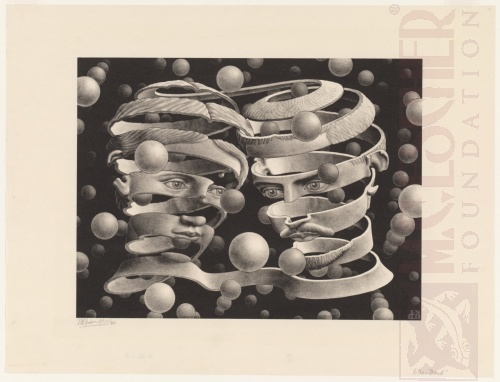
\includegraphics[width=\linewidth]{fig/escher/bound-of-union.jpg}
	\caption{\href{https://mcescher.com/gallery/most-popular/\#iLightbox[gallery\_image\_1]/23}{\emph{Bond of Union}}, M. C. Escher, \textcopyright~The M.C. Escher Company.}
\end{marginfigure}
"Duality@@CQ" takes its name from the fact that \Cref{prop:containment-hom} can be simply rephrased as
``the preordered set of "conjunctive queries" over $\sigma$ under
"containment" is \emph{dually isomorphic} to the preordered set of "relational databases"
over $\sigma$ under the homomorphism ordering.'' Symbolically: 
\[
	\tup{\kl[CQ]{\textrm{CQ}_\sigma},\; \contained }
	\isom
	\tup{\kl[relational database]{\textrm{RelDb}_\sigma},\; \cohomto }.
\]
Naturally, to go from "relational databases" to "conjunctive queries",
we associate to any "pointed relational database" $\tup{\?G, \bar g}$
a ""canonical conjunctive query"" $\gamma(\bar g)$ with one "atom"
$\+R_{(k)}(x_1,\hdots,x_k)$ for every "hyperedge" $\tup{x_1,\hdots,x_k} \in \+R_{(k)}(\?G)$.
This map is precisely the inverse of the construction defining "canonical database@@cqs@@cq".

This dual isomorphism has many consequences: essentially every theory that deals with
"relational databases" can be applied to study "conjunctive queries"!

\begin{corollary}[{of "duality@@CQ" and \Cref{prop:equiv-core-isomorphic}}]
	Two "conjunctive queries" are "semantically equivalent" "iff"
	the "core" of their "canonical database@@cq" are "isomorphic".
\end{corollary}

\paragraph*{Graphical depiction of the preordered set of relational databases.}
Note that for each "conjunctive query" $\gamma(\bar x)$, the class of
"pointed relational databases" $\tup{\?D, \bar d}$ satisfying the query
is \AP""closed under homomorphisms"", "ie"
\[
	\text{if}\quad \tup{\?D, \bar d} \FOmodels \gamma(\bar x)
	\quad\text{and}\quad \tup{\?D, \bar d} \homto \tup{\?D', \bar d'}
	\quad\text{then}\quad \tup{\?D', \bar d'} \FOmodels \gamma(\bar x).
\]
We represent the preordered set of "relational databases" ordered by $\homto$ as follows:
each equivalence class of "homomorphically equivalent" "relational databases" is
represented by a single point. In other words, points are in one-to-one correspondence
with "cores". Then, we represent a point $\core{\?G}$ below another point $\core{\?D}$
whenever $\core{\?G} \homto \core{\?D}$.
For "Boolean queries", this ordering%
\footnote{Formally, from the preordering over "relational databases" we obtained a partial
order over the quotient of "relational databases" by the equivalence class induced by $\homto$,
which happens to be the poset of "cores". Hence, we will interchangeably
use to terms \emph{preordering} and \emph{(partial) ordering}.}
admits a unique minimal element, which is the empty database.
For "non-Boolean queries", there is also a minimal "relational database" with
no facts, but that has constants.
Similarly, there is always a unique maximal element: the "database@@rel" with
a unique vertex $x$ and such that $\+R_{(k)}(x,\dotsc,x)$ holds for
every $\+R_{(k)} \in \sigma$, and all constants are interpreted as $x$.
We now prove that this poset has a non-trivial structure, provided that the "signature"
is itself non-trivial.

\begin{proposition}
	\AP\label{prop:poset-reldb}
	Assume that $\sigma$ contains at least one symbol of arity at least 2.
	The poset of "relational databases"
	admits infinite chains, infinite co-chains and infinite antichains.
\end{proposition}

\begin{figure}
	\centering
	\begin{tikzpicture}
		\foreach \i in {0,...,5} {
			\pgfmathtruncatemacro\j{mod(\i, 3)}
			\node[vertex, draw=c\j, fill=c\j, fill opacity=.4] (s\i) at (\i*360/6: 1.2cm) {};
		}
		\foreach \i in {0,...,5} {
			\pgfmathtruncatemacro\ip{mod(\i+1, 6)}
			\draw[edge] (s\i) to (s\ip);
		}

		\foreach \i in {0,1,2} {
			\node[vertex, draw=c\i, fill=c\i, fill opacity=.4] (t\i) at ($(\i*360/3: .9cm)+(5, 0)$) {};
		}
		\foreach \i in {0,1,2} {
			\pgfmathtruncatemacro\ip{mod(\i+1, 3)}
			\draw[edge] (t\i) to (t\ip);
		}
	\end{tikzpicture}
	\caption{\AP\label{fig:prelim-db-cycles} The "graphs@@dir" $\?C_6$
	(left) and $\?C_3$ (right) and a "homomorphism" from the former
	to the latter, described by colour coding.}
\end{figure}
\begin{proof}
	For the sake of simplicity, we assume that we actually have
	a binary predicate: this assumption is "wlog" since we can encode the binary 
	relation used in these constructions into any $k$-ary
	relation provided that $k \geq 2$ by encoding $\+E(x,y)$
	as $\+R_{(k)}(x,y,\dotsc,y)$.

	Clearly, "directed paths" provide an infinite chain
	\[
		\pathGraph{1} \homto \pathGraph{2} \homto \cdots
			\homto \pathGraph{n} \homto \pathGraph{n+1} \homto \cdots.
	\]
	We now let $\?C_n$ ($n\in\Np$) denote the directed cycle with domain $\ZnZ{n}$
	and with an edge from $i$ to $j$ "iff" $i+1 = j$, see \Cref{fig:prelim-db-cycles}.
	It is then routine to check that for $n,m\in\Np$, we have $\?C_n \homto \?C_m$
	"iff" $n$ is a multiple of $m$. In particular,%
	\footnote{In fact, we obtain a \emph{projective system}. We will discuss
	projective limits in \todo{ref conclu}.}
	we have
	\[
		\?C_1 \cohomto \?C_2 \cohomto \?C_4 \cohomto \cdots \cohomto \?C_{2^n} \cohomto \?C_{2^{n+1}} \cohomto \cdots.
	\]
	Finally, $\tup{\?C_p}_{p \text{ prime}}$ is an infinite antichain.
\end{proof}

\begin{figure}
	\centering
	\begin{tikzpicture}[
		font=\footnotesize,
		every node/.style={inner sep=0pt,outer sep=0pt}
	]
		\begin{luacode}
-- parameters to tweak
-- nb of nodes in the lattice
width = 17 -- half-width
height = 17 -- half-height
-- height and width (in cm) of the tikzpicture
display_width = 10
display_height = 10
-- decay rates 
x_opacity_decay = 0.3
y_opacity_decay = 1.5
pos_decay = 1.5

dx = display_width / (2 * width)
dy = display_height / (2 * height)

function grid_to_picture_x(x)
	-- returns the position in the picture from the coordinates in the grid
	return x * dx * (math.abs(x)/width)^(pos_decay-1)
end 
function grid_to_picture_y(y)
	-- returns the position in the picture from the coordinates in the grid
	return y * dy * (math.abs(y)/height)^(pos_decay-1)
end

function is_part_of_grid(x,y)
	in_square = x >= -width and x <= width and y >= -height and y <= height
	in_check = (x+y)%2 ~= 0
	in_diamond = math.abs(x) <= height - math.abs(y)
	return in_square and in_check and in_diamond
end

function is_above(x1,y1,x2,y2) -- check if (x1,y1) is above (x2,y2)
	if y1 < y2 then
		return false
	end
	delta_y = y1 - y2 -- >= 0
	delta_x = math.abs(x2 - x1)
	return (delta_x <= delta_y)
end

function get_color(x,y)
	if y - x == 17 then
		return "c0"
	elseif y + x == -17 then
		return "c2"
	else
		return "black" 
	end
end

function process_opacity(x)
	return (1/(1+math.exp(3.5-20*x)))
end

function get_opacity(x,y)
	if y == 0 then
		return process_opacity(0)
	elseif math.abs(y) == height then
		return process_opacity(1)
	elseif math.abs(y) == 1 and math.abs(x) < width-1 then
		return process_opacity(0.01)
	elseif math.abs(x) == 1 and math.abs(y) < height-1 then
		return process_opacity(0.02)
	elseif math.abs(x) == 0 and math.abs(y) < height-1 then
		return process_opacity(0)
	else
		x_opac = (math.abs(x)/width)^x_opacity_decay
		y_opac = (math.abs(y)/height)^y_opacity_decay
		return process_opacity(x_opac * y_opac)
	end
end

function get_scale(x,y)
	return 2*get_opacity(x,y)^0.3
end

function get_edge_color(x1,y1,x2,y2)
	c1 = get_color(x1,y1)
	c2 = get_color(x2,y2)
	if c1 == c2 then
		return c1
	else 
		return "black"
	end
end

function get_edge_opacity(x1,y1,x2,y2)
	o1 = get_opacity(x1,y1)
	o2 = get_opacity(x2,y2)
	return math.min(o1,o2)
end

-- define coordinates
for x = -width,width do
	for y = -height,height do
		if is_part_of_grid(x,y) then
			tex.print(string.format("\\coordinate (%i %i) at (%.4f, %.4f) {};", x, y, grid_to_picture_x(x), grid_to_picture_y(y)))
		end
	end 
end 
-- draw edges
for x = -width,width do
	for y = -height,height do
		if is_part_of_grid(x,y) then
			above = {{x-1,y+1}, {x+1, y+1}}
			for _, coord in ipairs(above) do 
				x2, y2 = coord[1], coord[2]
				if is_part_of_grid(x2,y2) then
					tex.print(string.format("\\draw[color=%s, opacity=%.4f] (%i %i) to[-] (%i %i);", get_edge_color(x,y,x2,y2), get_edge_opacity(x,y,x2,y2), x, y, x2, y2))
				end
			end
		end
	end 
end 
-- draw grid
for x = -width,width do
	for y = -height,height do
		if is_part_of_grid(x,y) then
			-- white background
			tex.print(string.format("\\node[circle,fill=white, minimum size=%.4f pt] at (%i %i) {};", get_scale(x,y), x, y))
			-- proper colour
			tex.print(string.format("\\node[circle,fill=%s, minimum size=%.4f pt, opacity=%.4f] at (%i %i) {};", get_color(x,y), get_scale(x,y), get_opacity(x,y), x, y))
		end
	end 
end 

\end{luacode}
		\node[above left=2pt of 0 17, color=c0] {$\?C_1$};
		\node[above left=2pt of -1 16, color=c0] {$\?C_2$};
		\node[above left=2pt of -2 15, color=c0] {$\?C_4$};
		\node[above left=2pt of -4 13, color=c0] {\rotatebox{-30}{$\vdots$}};
		\node[above left=2pt of -6 11, color=c0] {$\?C_{2^n}$};
		\node[above left=2pt of -7 10, color=c0] {$\?C_{2^{n+1}}$};
		\node[above left=2pt of -9 8, color=c0] {\rotatebox{-45}{$\vdots$}};

		\node[below left=2pt of 0 -17, color=c2] {$\emptyset$};
		\node[below left=2pt of -1 -16, color=c2] {$\?P_1$};
		\node[below left=2pt of -2 -15, color=c2] {$\?P_2$};
		\node[below left=2pt of -4 -13, color=c2] {\rotatebox{30}{$\vdots$}};
		\node[below left=2pt of -6 -11, color=c2] {$\?P_{n}$};
		\node[below left=2pt of -7 -10, color=c2] {$\?P_{n+1}$};
		\node[below left=2pt of -9 -8, color=c2] {\rotatebox{45}{$\vdots$}};

		\node[circle, fill=white, minimum size=4pt] at (4 -9) {};
		\node[circle, fill=c1, opacity=1, minimum size= 4pt, outer sep=1mm] at (4 -9) {};

		\node[color=c1, align=left, text width=3.8cm, outer sep=1mm] at (3.5, -5) (label-cdb)
			{"\textcolor{c1}{canonical database}@canonical database" $\?G$ of a
			"\textcolor{c1}{Boolean conjunctive query}@Boolean conjunctive query" $\gamma$};
		\draw[draw=c1, semithick] (label-cdb) edge[->,out=90,in=-90] ($(4 -9)+(0, -.1)$);
		\draw[draw=c1, semithick, decorate,decoration={brace,amplitude=5pt,raise=.5em}]
  			(0 17) -- (15 2)
			node[color=c1, midway, above right=5mm, align=left, text width=3.8cm]
				{semantics of $\gamma$};
	\end{tikzpicture}
	\caption{\AP\label{fig:poset-reldb} The poset of "relational databases" over a "signature"
	containing at single binary "predicate", where "homomorphisms" go from bottom to top.
	An infinite chain is represented in red, and an infinite co-chain in blue.
	A large yellow dot represents the "canonical database@@cq" of a "conjunctive query",
	while the semantics of this "conjunctive query" is represented with normal-size yellow dots.}
\end{figure}
Based on \Cref{prop:poset-reldb}, we provide an illustration of the ordered set
of "relational databases" in \Cref{fig:poset-reldb}. Notice that, since the semantics
of "conjunctive queries" is closed under "homomorphisms", they are represented by an upper-closed set. Moreover, this set has a unique minimum, corresponding to its "canonical database@@cq".
Notice how this representation naturally represents the concept of "duality@@CQ":
\begin{itemize}
	\item points of the poset ("ie" "relational databases") are in natural
		bijection with upper-closed set that admit a minimum ("ie" "conjunctive queries");
	\item a "conjunctive query" is "contained" in another "iff"
		the "canonical database@@cq" of the first is below that of the second
		in \Cref{fig:poset-reldb}.
\end{itemize}

\begin{marginfigure}
	\centering
	\directlua{width = 2.3; height = 1.4}
\input{tikz/prelim-databases/abstract-lattice.lua}%do not indent!!!
	\begin{tikzpicture}[every node/.style={inner sep=0pt,outer sep=0pt},font=\footnotesize]
		\directlua{draw_lattice()}
		\begin{scope}
			\directlua{make_clip()}
			\directlua{draw_cq(.5, -.6, 'c0', 'x')}
			\directlua{draw_cq(.65, .2, 'c2', 'y')}
			\node[below=2pt of x, c0] {$\gamma$};
			\node[below=2pt of y, c2] {$\delta$};
		\end{scope}
	\end{tikzpicture}
	\caption{
		\AP\label{fig:poset-reldb-simple}
		A more abstract view of the poset of "relational databases":
		we represent two "conjunctive queries" $\gamma$ (in red) and $\delta$ (in blue).
		The semantics of each query is represented by a filled diamond,
		and its "canonical database@@cq" by a large dot.
	}
\end{marginfigure}
For the sake of simplicity---and compilation time of this document!---,
we abstract the picture of \Cref{fig:poset-reldb} into \Cref{fig:poset-reldb-simple}.

\begin{remark}
	\label{rk:database-vs-structures}
	À propos "relational databases" "vs" "relational structures",
	these posets are actually isomorphic 
	since a "relational structure" is always "homomorphically equivalent"
	to the structure in which we removed "isolated vertices".
\end{remark}

\paragraph*{The Distributive Lattice of Relational Databases.}

\Cref{prop:poset-reldb} shows that the poset of "relational databases" has a somewhat
complex structure, in the sense that it has infinite height, co-height and width.
However, we next show that it has a rich algebraic structure.

\begin{marginfigure}
	\centering
	\begin{tikzcd}[row sep=huge]
		\tup{\?D_1,\bar d_1} &[-4em] &[-4em] \tup{\?D_2,\bar d_2} \\ 
		& \tup{\?D_1,\bar d_1} \prodstruct \tup{\?D_2,\bar d_2}
			\ar[ul, "\projHom{1}" swap] \ar[ur, "\projHom{2}"]
		& \\
		& \tup{\?U, \bar u} \ar[u, "g", dashed]
			\ar[uul, "f_1", bend left] \ar[uur, "f_2" swap, bend right]
		&
	\end{tikzcd}
	\caption{\AP\label{fig:cartesian-product-diagram} Universal property satisfied
	by the "Cartesian product".}
\end{marginfigure}
In light of \Cref{rk:database-vs-structures}, the "Cartesian product"
of two "relational databases" $\tup{\?D_1,\bar d_1}$ and $\tup{\?D_2,\bar d_2}$
whose tuples have the same arity
is well-defined: we consider their product $\tup{\?D_1,\bar d_1} \prodstruct \tup{\?D_2,\bar d_2}$
as "relational structures", and remove all "isolated vertices".
We slightly abuse the notation and still denote this product by $\reintro*\prodstruct$.
It is routine to check that this "Cartesian product" in indeed a Cartesian product in
the categorical sense, "ie" that it satisfies the universal property
that it has "homomorphisms" $\projHom{1}$ and $\projHom{2}$ to both $\tup{\?D_1,\bar d_1}$ and $\tup{\?D_2,\bar d_2}$, and that moreover it is the smallest object satisfying this property,
in the sense that for every "relational database" $\tup{\?U, \bar u}$ with "homomorphisms"
$f_1$ and $f_2$ to $\tup{\?D_1,\bar d_1}$ and $\tup{\?D_2,\bar d_2}$, 
then there exists a unique "homomorphism" $\?G$ from $\tup{\?U, \bar u}$ to
$\tup{\?D_1,\bar d_1} \prodstruct \tup{\?D_2,\bar d_2}$ such that
the diagram of \Cref{fig:cartesian-product-diagram} commutes:
this "homomorphism" $\?G$ is actually $f_1 \times f_2\colon u \mapsto \tup{f_1(u), f_2(u)}$.
Going back to the poset structure, this implies that any pair of points must have an infimum.
\begin{fact}
	Given two finite "relational databases", their "Cartesian product"
	is their greatest lower bound in the poset of "relational databases"
	ordered by $\homto$.
\end{fact}

\begin{marginfigure}
	\centering
	\directlua{width = 2.3; height = 1.4}
\input{tikz/prelim-databases/abstract-lattice.lua}%do not indent!!!
	\begin{tikzpicture}[x=1cm, y=1cm, every node/.style={inner sep=0pt,outer sep=0pt}, font=\footnotesize]
		\directlua{draw_lattice()}
		\begin{scope}
\begin{luacode}
			x0 = 0
			y0 = -.5
			dist = .5
			slope = height/width
			draw_db(x0-dist, y0+dist*slope, 'cBlue', '1')
			draw_db(x0+dist, y0+dist*slope, 'cRed', '2')
			draw_db(x0, y0, 'cYellow', 'prod')
			draw_db(x0, y0+2*dist*slope, 'cPurple', 'union')
\end{luacode}
			\node[left=3.5pt of 1, cBlue] {$\?D_1$};
			\node[right=3.5pt of 2, cRed] {$\?D_2$};
			\node[below=3.5pt of prod, cYellow] {$\?D_1 \prodstruct \?D_2$};
			\node[above=3.5pt of union, cPurple] {$\?D_1 \disunion \?D_2$};
			\draw (prod) edge[->] (1);
			\draw (prod) edge[->] (2);
			\draw (1) edge[->] (union);
			\draw (2) edge[->] (union);
		\end{scope}
	\end{tikzpicture}
	\caption{
		\AP\label{fig:distributive-lattice-rel-db}
		The distributive lattice structure of "relational databases": 
		we represent two "structures", as well as their least upper bound
		and greatest lower bound.
	}
\end{marginfigure}
Similarly, the "disjoint union" satisfies the property dual to \Cref{fig:cartesian-product-diagram}.
\begin{fact}
	Given two finite "relational databases", their "disjoint union"
	is their least upper bound in the poset of "relational databases"
	ordered by $\homto$.
\end{fact}

\begin{figure}
	\centering
	\newrobustcmd{\halfcircle}[2]{
		\begin{scope}[shift=(#1)]
			\fill[#2] (0,0) -- (135:3.4pt) arc (135:315:3.4pt) -- cycle;
			\fill[white] (0,0) -- (135:2.4pt) arc (135:315:2.4pt) -- cycle;
			\fill[#2, fill opacity=.4] (0,0) -- (135:2.4pt) arc (135:315:2.4pt) -- cycle;
		\end{scope}
	}
	\begin{tikzpicture}
		\node[vertex, draw=cGrey, fill=cGrey, fill opacity=.4] (d0) at ($(0*360/2: .7cm)+(-1,0)$) {};
		\node[vertex, draw=cPurple, fill=cPurple, fill opacity=.4] (d1) at ($(1*360/2: .7cm)+(-1,0)$) {};
		\draw[edge, bend right] (d0) to (d1);
		\draw[edge, bend right] (d1) to (d0);

		\foreach \i in {0,1,2} {
			\node[vertex, draw=c\i, fill=c\i, fill opacity=.4] (t\i) at ($(\i*360/3: .9cm)+(7, 0)$) {};
		}
		\foreach \i in {0,1,2} {
			\pgfmathtruncatemacro\ip{mod(\i+1, 3)}
			\draw[edge] (t\i) to (t\ip);
		}

		\foreach \i/\c in {0/cGrey,1/cPurple,2/cGrey,3/cPurple,4/cGrey,5/cPurple} {
			\pgfmathtruncatemacro\im{mod(\i, 3)}
			\node[vertex, draw=c\im, fill=c\im, fill opacity=.4] (s\i) at ($(\i*360/6: 1.2cm)+(3, -2)$) {};
			\halfcircle{s\i}{\c}
		}
		\foreach \i in {0,...,5} {
			\pgfmathtruncatemacro\ip{mod(\i+1, 6)}
			\draw[edge] (s\i) to (s\ip);
		}
		\draw[rounded corners=4pt, dashed, cGrey] (-2.3,-1.2) rectangle (.3,1.2);
		\draw[rounded corners=4pt, dashed, cGrey] (5.8,-1.5) rectangle (8.5,1.5);
		\draw[rounded corners=4pt, dashed, cGrey] (1.3,-3.7) rectangle (4.7,-.3);

		\begin{scope}[yshift=2cm,xshift=2cm]
			\node[vertex, draw=cGrey, fill=cGrey, fill opacity=.4] (2d0) at (0*360/2: .7cm) {};
			\node[vertex, draw=cPurple, fill=cPurple, fill opacity=.4] (2d1) at (1*360/2: .7cm) {};
			\draw[edge, bend right] (2d0) to (2d1);
			\draw[edge, bend right] (2d1) to (2d0);

			\foreach \i in {0,1,2} {
				\node[vertex, draw=c\i, fill=c\i, fill opacity=.4] (2t\i) at ($(\i*360/3: .9cm)+(2, 0)$) {};
			}
			\foreach \i in {0,1,2} {
				\pgfmathtruncatemacro\ip{mod(\i+1, 3)}
				\draw[edge] (2t\i) to (2t\ip);
			}
			\draw[rounded corners=4pt, dashed, cGrey] (-1.3,-1.5) rectangle (3.5,1.5);
		\end{scope}
		\caption{\AP\label{fig:distributive-lattice-rel-db-concrete}
			Two "databases@@rel" (left and right), their "Cartesian product" (below)
			and "disjoint union" (above).
		}
	\end{tikzpicture}
\end{figure}
Put together, these facts imply that the poset of "relational databases" is
actually a bounded lattice, as depicted in \Cref{fig:distributive-lattice-rel-db,fig:distributive-lattice-rel-db-concrete}.
It is moreover distributive
since the isomorphism (and hence "homomorphic equivalence")
\[
	\?A \prodstruct (\?B \disunion \?C) \isom (\?A \prodstruct \?B) \disunion (\?A \prodstruct \?C)
\]
holds for any "databases@@rel" $\?A$, $\?B$ and $\?C$.
Then, by "duality@@CQ", we get that the poset of "conjunctive queries"
under "containment" is also a distributive lattice!
We shall see that the greatest lower bound and least upper bound
have a natural logical interpretation, and that moreover
this structure of distributive lattice will help us
deal with "CQs": and in particular
solve the "synthesis problem". 


\paragraph*{The Distributive Lattice of Conjunctive Queries.}

Given two "CQs" $\gamma(\bar x)$ and $\delta(\bar y)$,
where $\bar x$ and $\bar y$ have the same arity, we define
their \AP""disjoint conjunction"", denoted by
$\gamma(\bar x) \intro*\disconj \delta(\bar y)$,
to be the "CQs" obtained by taking the "disjoint union" of "atoms" 
of the "CQs" and then identifying the elements of $\bar x$ and $\bar y$ pointwise.
For instance, letting $\gamma(x) \defeq x \atom{a} y$ be the query
asking for all elements with an outgoing $a$-edge,
and $\delta(x) \defeq x \atom{b} y$ be the query
asking for all elements with an outgoing $a$-edge,
then their "disjoint conjunction" $\gamma(x) \disconj \delta(x)$ is
\[
	\alpha(x) \defeq x \atom{a} y \land x \atom{b} y',
\]
which outputs all elements with both an outgoing $a$-edge and an outgoing $b$-edge.%
\footnote{As for "disjoint union", the name "disjoint conjunction" is slightly abusive
but justified by its universal property.}

\begin{fact}
	The "canonical database@@cq" of the "disjoint conjunction"
	equals the "disjoint union" of the "canonical database@@cqs@@cq".
	By "duality@@CQ", it follows that
	the "disjoint conjunction" is the greatest lower bound
	of two "CQs".%
	\footnote{Careful: "duality@@CQ" is precisely a \emph{dual} isomorphism,
	"ie" it reverses the order. Hence, a least upper bound ("disjoint union")
	becomes a greatest lower bound ("disjoint conjunction").}
\end{fact}

The other operator (the dual of "Cartesian product")
does not have such a nice intuitive interpretation---however
it does not mean that it will be less useful, on the contrary!
While "conjunctive queries" are not closed under
semantical union---we will see this in \Cref{sec:prelim-db-ucq}---, this operator
acts as the best approximation of it.

\begin{definition}
	We define the \AP""weak union"" \AP$\intro*\weakunion$ of two "CQs"
	with the same number of "output variables"
	as the "canonical CQ" of the "Cartesian product" of their "canonical database@@cqs@@cq".
\end{definition}

By construction, it is their greatest upper bound,
in the sense that
$\gamma(\bar x) \contained \gamma(\bar x) \weakunion \delta(\bar y)$,
$\delta(\bar y) \contained \gamma(\bar x) \weakunion \delta(\bar y)$,
and $\gamma(\bar x) \weakunion \delta(\bar y)$ is the smallest "CQ" satisfying this property.

For instance, if $\gamma() \defeq x \atom{a} y$ asks for the existence of an $a$-edge
and $\delta() \defeq x \atom{b} y$ asks for a $b$-edge,
then $\gamma() \weakunion \delta()$ is the empty "CQ",
"ie" the "CQ" that always true: knowing that a "database@@graph" contains either an $a$-edge
or a $b$-edge is as good as knowing nothing in terms of "CQ" expressivity.
On the other hand, if $\gamma(x) \defeq x \atom{a} y \atom{b} z$ outputs the source of all 
$ac$-paths and $\delta(x) \defeq x \atom{a} y \atom{c} z$ outputs the source of all $bc$-paths,
then $\gamma(x) \weakunion \delta(x)$ will be "homomorphically equivalent" to
$\upsilon(x) \defeq x \atom{a} y$ which outputs all sources of $a$-edges.

\begin{marginfigure}
	\centering
	\directlua{width = 2.3; height = 1.4}
\input{tikz/prelim-databases/abstract-lattice.lua}%do not indent!!!
	\begin{tikzpicture}[x=1cm, y=1cm, every node/.style={inner sep=0pt,outer sep=0pt}, font=\footnotesize]
		\directlua{draw_lattice()}
		\begin{scope}
\begin{luacode}
			make_clip()
			x0 = 0
			y0 = -.5
			dist = .5
			slope = height/width
			draw_cq(x0, y0, 'cYellow', 'prod')
			draw_cq(x0-dist, y0+dist*slope, 'cBlue', '1')
			draw_cq(x0+dist, y0+dist*slope, 'cRed', '2')
			draw_cq(x0, y0+2*dist*slope, 'cPurple', 'union')
\end{luacode}
			\node[left=3.5pt of 1, cBlue] {$\gamma_1$};
			\node[right=3.5pt of 2, cRed] {$\gamma_2$};
			\node[below=3.5pt of prod, cYellow] {$\gamma_1 \weakunion \gamma_2$};
			\node[above=3.5pt of union, cPurple!50!black] {$\gamma_1 \disconj \gamma_2$};
		\end{scope}
	\end{tikzpicture}
	\caption{
		\AP\label{fig:distributive-lattice-cq}
		The distributive lattice structure of "Boolean conjunctive queries": 
		we represent two "structures", as well as their least upper bound
		and greatest lower bound, and the natural homomorphism they come equipped with
		(projections and canonical embeddings).
	}
\end{marginfigure}
The distributive lattice structure of "conjunctive queries"
is depicted in \Cref{fig:distributive-lattice-cq}. Observe how this
choice of representation makes obvious the fact that
(1) the "disjoint conjunction" of two "CQs" is actually its
conjunction in the semantical sense, but (2)
their "weak union" is strictly bigger than their semantical union,
unless we are in a degenerate case.

We summarize the properties of the two distributive lattices
in \Cref{tab:distributive-lattices}. Note that all notions
occurring in this table, be it the orders or the binary operators,
require the "CQs" to the same number of "output variables",
and the (pointed) "relational databases" to have tuples of the same size,
and so in fact we obtain two lattices for every possible arity/tuple size.
% Note also motivates the somewhat counter-intuitive definition of the
% "disjoint union" for "structures" over "signatures" that are not
% "purely relational@@signature".

\begin{table}
	\centering
	\begin{tabular}{ccc}
		\toprule
		 & "Conjunctive Queries" & "Relational Databases" \\ \midrule
		\multirow{2}{*}{preorder} & \multirow{2}{*}{"containment" $\contained$} & existence of\\
		& & "homomorphisms" $\homto$ \\
		least upper bound & "weak union" $\weakunion$ & "disjoint union" $\disunion$ \\
		greatest lower bound & "disjoint conjunction" $\disconj$ & "Cartesian product" $\prodstruct$ \\ 
		\multirow{2}{*}{greatest element} & \multirow{2}{*}{``true'' (empty "CQ")} & single vertex \\
		& & will all "hyperedges" \\
		\multirow{2}{*}{least element} & single variable & \multirow{2}{*}{empty "database@@rel"}
		\\
		& will all "hyperedges" & \\ \bottomrule
	\end{tabular}
	\caption{
		\AP\label{tab:distributive-lattices}
		The distributive lattices of "conjunctive queries" and "relational databases".
		By "duality@@CQ", one can go from one lattice to the \emph{opposite} of the other
		by taking "canonical database@@cqs@@cq" or "canonical conjunctive queries".}
\end{table}

Amongst bounded distributive lattices, the better behaved are
the Boolean algebras, in which every element has a complement.
In our case, this would be an operator $\neg$ "st" for every "database@@rel" $\?D$,
then $\?D \prodstruct {\neg \?D}$ would be "homomorphically equivalent" to
the empty database and $\?D \disunion {\neg \?D}$ to the greatest database,
consisting of a single vertex and all possible "hyperedges" over it.

\begin{proposition}
	The distributive lattice of "databases@@rel" (and hence of
	"conjunctive queries") does not admit complementation.
\end{proposition}

\begin{proof}
	Assume that the "signature" is non-trivial and let $\?D$ be a non-trivial "database@@rel",
	"ie" neither the least nor greatest element of the lattice.
	To ensure that $\?D \disunion {\neg \?D}$ is "homomorphical equivalent"
	to the greatest database, $\neg \?D$ must actually be "homomorphical equivalent" to 
	the greatest database itself,
	but then $\?D \prodstruct {\neg \?D}$ would be non-empty.
	Hence, $\neg \?D$ cannot exist.
\end{proof}

However, "conjunctive queries" still have a bit more structure: we shall
see that they are a Heyting algebra, namely that it is a bounded distributive lattice
with the extra property that for every $\gamma(\bar x)$ and $\delta(\bar y)$,
where $\bar x$ and $\bar y$ have the same arity, then there exists
a greatest element $\chi(\bar z)$ "st"
\[
	\gamma(\bar x) \disconj \chi(\bar y) \contained \delta(\Bar z). 
\]
This greatest element $\chi(\bar z)$ is denoted by \AP$\gamma(\bar x) \intro*\impH \delta(\bar y)$, and is called \emph{implication}.%
\footnote{Heyting algebras were introduced to model intuitionistic logic.
It is not hard to see that the implication $\phi \Rightarrow \psi$
does satisfy the property it is the greatest formula $\chi$
"st" $\phi \land \chi$ entails $\psi$.}

\begin{proposition}
	\!\footnote{The fact that "relational databases" and "conjunctive queries" form
	a bounded distributive lattice is folklore.}
	The bounded distributive lattice of "conjunctive queries" is actually
	a Heyting algebra.
\end{proposition}

\begin{proof}
	We use "duality@@CQ" to prove this and show that "relational databases" form a ``co-Heyting algebra'',
	in the sense that for any "database@@rel" $\tup{\?G, \bar g}$ and $\tup{\?D, \bar d}$,
	there exists a least element $\tup{\?X, \bar x}$ "st"
	\[
		\tup{\?G, \bar g} \disunion \tup{\?X, \bar x} \cohomto \tup{\?D, \bar d}:
	\]
	$\tup{\?X, \bar x}$ is actually obtained by taking the "disjoint union"
	of all "connected components" of $\tup{\?D, \bar d}$ 
	that cannot be "mapped homomorphically" to $\tup{\?G, \bar g}$.
	The operator $\impH$ can then be explicitly constructed by "duality@@CQ".
\end{proof}

By construction of $\impH$, it comes naturally equipped with some
form of Currying, in the sense that
\[
	\tup{\?A, \bar a}
	\FOmodels \gamma(\bar x) \impH \delta(\bar y)
	\quad\text{"iff"}\quad
	\tup{\?A, \bar a} \disunion \tup{\?G, \bar x}
	\FOmodels \delta(\bar y),
\]
for any "CQs" $\gamma(\bar x)$ and $\delta(\bar y)$
and any "relational database" $\tup{\?A, \bar a}$,
where $\tup{\?G, \bar x}$ denotes the "canonical database@@cq" of $\gamma(\bar x)$.
Similarly, as expected, we have
\[
	\gamma(\bar x) \disconj (\gamma(\bar x) \impH \delta(\bar y))
	\semequiv
	\delta(\bar y).
\]

In \Cref{sec:prelim-db-static-analysis-cq,sec:prelim-db-ucq},
we will apply some of the theory we developed here
to better understand the expressivity of \emph{conjunctive queries}.

\subsection{Static Analysis of Conjunctive Queries}
\label{sec:prelim-db-static-analysis-cq}

\paragraph*{Minimization.}
As we have already seen, the first consequence of "duality@@CQ" is that
"containment" and "semantical equivalence" are both
decidable, see \Cref{coro:prelim-db-containment-cq}.
We shall now see that the rich theory of "relational structures",
and in particular the concept of "cores" trivializes the question of minimization.

Fix a "relational signature" $\sigma$.
A ""subquery@@CQ"" of $\gamma(\bar x)$ is any "CQ" over $\sigma$
obtained by removing variable and/or atoms from $\gamma$:
to ensure that we still obtain a "CQ" over $\sigma$, "output variables" 
cannot be removed.
In terms of "duality@@CQ", this amounts to taking the "canonical conjunctive query" of
a "substructure" of the "canonical database@@cq".%
\footnote{Careful: if $\gamma'$ is a subquery of $\gamma$, then $\gamma \contained \gamma'$!
The fewer constraints there is, the easier it is to satisfy them…}
We then say that a class $\+C$ of "conjunctive queries" over $\sigma$ is ""monotone@@classCQ""
if for any "CQ" $\gamma(\bar x) \in \+C$, for any "subquery@@CQ" $\gamma'(\bar x)$ of
$\gamma(\bar x)$, we must have $\gamma'(\bar x) \in \+C$.
"Monotone classes of CQs" naturally model the notion of ``simplicity'', in the sense that
a "CQ" is ``simple'' "wrt" $\+C$ whenever it belongs to $\+C$. The "monotonicity@@classCQ"
assumption precisely assures that the class formalizes an idea of ``simplicity''
and not ``the "CQ" has exactly fourteen atoms, two ternary "hyperedges", three legs,
a moustache and a mustard watch.''
Typical examples of "monotone classes of CQs" include:
\begin{itemize}
	\item "CQs" with at most $k \in \N$ "atoms",
	\item "CQs" with at most $k$ variables,
	\item "CQs" of "tree-width" at most $k$ (defined in \Cref{sec:prelim-db-tw}),
	\item "CQs" of "path-width" at most $k$,
	\item "CQs" in which all "cliques" are of size at most $k$, etc.
\end{itemize}

We define the ""core@@CQ"" of a "conjunctive query", still denoted by $\intro*\coreCQ{-}$,
to be the "canonical conjunctive query" of the "core" of its "canonical database@@cq".
\begin{proposition}
	\AP\label{prop:minimization-CQ}
	Let $\gamma(\bar x)$ be a "conjunctive query" and $\+C$ be
	a "monotone class of CQs". Then $\gamma(\bar x)$ is "semantically equivalent"
	to a "CQ" in $\+C$ if, and only if, its "core@@CQ" $\coreCQ{\gamma}(\bar x)$
	belongs to $\+C$.
\end{proposition}

\begin{proof}
	This follows from \Cref{prop:equiv-core-isomorphic}
	and the fact that the "core" of a "structure" is always
	a "substructure" of it.
\end{proof}

Not only does this imply that we can solve the $\+C$-minimization problem,
but actually that all these problems can be solved simultaneously,
in the sense that if a solution exists to each problem, then a common solution exists!

\decisionproblem{""CQ minimization problem over $\+C$""}{
	A "conjunctive query".
}{
	Is it "semantically equivalent" to a "CQ" of $\+C$?
}

\begin{corollary}
	\label{coro:decision-minimization-cq}
	For each "monotone class of CQs" $\+C$, assumed to be described as an oracle,
	the ""CQ minimization problem over $\+C$"" is "NP".
	Furthermore, it is "NP"-hard for some classes $\+C$.
\end{corollary}

\begin{proof}
	\proofcase{Upper bound.}
	A naïve algorithm would be to first compute the "core", and using the oracle
	to test if it belongs to $\+C$.
	However, computing the "core" is not in "NP": intuitively,
	we first need to guess a substructure that is "homomorphically equivalent"
	to the whole---which is "NP"---,
	and then check that no strictly smaller structure satisfies the property---which is "coNP".%
	\footnote{In fact, deciding if a "structure" is a "core" is actually
	"coNP"-complete, even for undirected graphs, \cite[Theorem~7]{HellNesetril1992Core}.}
	So, let not be naïve! We start with a "conjunctive query"
	$\gamma(\bar x)$, guess a "subquery" $\gamma'(\bar x)$,
	and then check if (1)%
	\footnote{In fact $\gamma \contained \gamma'$ always holds so
	it suffices to check that $\gamma' \contained \gamma'$.}
	$\gamma'(\bar x) \semequiv \gamma(\bar)$ and
	if (2) $\gamma'(\bar x) \in \+C$.
	The algorithm is clearly in "NP", and moreover it is correct
	by \Cref{prop:equiv-core-isomorphic} and monotonicity.

	\proofcase{Lower bound.} We prove that the minimization problem
	is "NP"-hard for the class $\+C$ of "conjunctive queries" with
	at most $3$ variables.
	In fact, by "duality@@CQ", we rather prove that the problem
	of, given a "structure", deciding if it is "homomorphically equivalent"
	to a "structure" with at most $3$ vertices is "NP"-hard.
	We reduce "$3$-colourability" to this latter problem.
	Given an instance $\?G$ of "$3$-colourability", we reduce
	it to:
	\begin{itemize}
		\item $\?G \disunion \clique{3}$ if $\?G$ does not contain any self-loop;
		\item any negative instance otherwise, "eg" $\clique{4}$.
	\end{itemize}
	If $\?G$ is "$3$-colourable", then it has no self-loop
	and moreover $\?G \homto \clique{3} \homto \clique{3}$
	and hence $\?G \disunion \marked{\clique{3}} \homto \clique{3}$, 
	from which we get that $\?G \disunion \clique{3} \semequiv \clique{3}$,
	and hence $\?G \disunion \clique{3}$ is "semantically equivalent" to a "structure"
	with at most $3$ vertices.
	Conversely, assume that the right-hand side of the reduction is "semantically equivalent" to a 
	"structure" with at most $3$ vertices. Then $\?G$ does not contain any self-loop
	and moreover, we get that $\?G \disunion \clique{3}$ is "homomorphically equivalent"
	to a structure with 3 vertices.
	In particular, we get a "homomorphism" from $\?G$ to a structure with 3 vertices,
	and from the assumption that $\?G$ does not contain any self-loop,
	we actually get a "homomorphism" from $\?G$ to $\clique{3}$.
	This concludes the reduction.%
	\footnote{The trick used for the lower bound, 
	namely that of reducing a "homomorphism"/"containment" problem
	to a minimization problem "via" a "disjoint union", will be used in a
	much trickier way in \Cref{ch:minimization-CRPQ}
	to prove "ExpSpace" lower bounds on the "minimization problem for CRPQs", 
	see \label{sec:minimization-lowerbounds,apdx-sec:lowerbound-variables}.}
\end{proof}

\begin{marginfigure}
	\centering
	\directlua{width = 2.3; height = 1.4}
\input{tikz/prelim-databases/abstract-lattice.lua}%do not indent!!!
	\begin{tikzpicture}[x=1cm, y=1cm, every node/.style={inner sep=0pt,outer sep=0pt}, font=\footnotesize]
		\directlua{draw_lattice()}
		\begin{scope}
\begin{luacode}
			make_clip()
			x0 = 0
			y0 = -.5
			dist = .5
			slope = height/width
			draw_cq(x0+.1, y0-.2, 'cGrey', 'cq')
			draw_db(x0-dist, y0+dist*slope, 'cBlue', 'p1')
			draw_db(x0+dist, y0+dist*slope, 'cBlue', 'p2')
			draw_db(x0-1.5, y0+.5, 'cRed', 'n1')
			draw_db(x0-.3, y0-.2, 'cRed', 'n2')
			draw_db(x0+.67, y0-.4, 'cRed', 'n3')
\end{luacode}
			\node[above=3.5pt of p1, cBlue] {$\?D^+_1$};
			\node[above=3.5pt of p2, cBlue] {$\?D^+_2$};
			\node[below=3.5pt of cq, cGrey!70!black] {$\gamma$};
			\node[below=3.5pt of n1, cRed] {$\?D^-_1$};
			\node[below=3.5pt of n2, cRed] {$\?D^-_2$};
			\node[above=3.5pt of n3, cRed] {$\?D^-_3$};
		\end{scope}
	\end{tikzpicture}
	\caption{
		\AP\label{fig:prelim-db-ex-synthesis}
		An instance of the "synthesis problem for CQs", as well as one valid
		solution for this instance.
	}
\end{marginfigure}
We now turn to the "synthesis problem", also called \emph{passive learning},
\emph{reverse engineering}. The idea behind the problem is to infer a
"query@@sem" from examples: these examples take the form
of models, taking the form of "pointed relational databases", together
with the knowledge of whether this model should be part of the "query@@sem"
(\emph{positive examples}) or not (\emph{negative examples}),
see \Cref{fig:prelim-db-ex-synthesis}.%
\footnote{For the sake of readability, we use the notations
for "Boolean queries" and non-"pointed databases@@rel".
However, all results extend trivially to the non-Boolean case.}

\decisionproblem{""Synthesis Problem for CQs""}{
	Integers $n,p\in \Np$, and
	"pointed relational databases"
	$\?D^+_1$, $\dotsc$, $\?D^+_p$, 
	$\?D^-_1$, $\dotsc$, $\?D^-_n$.
}{
	Is there a "conjunctive query" $\gamma$ "st"
	$\?D^+_i \FOmodels \gamma$ for all $i\in \intInt{1,p}$
	and $\?D^-_j \notFOmodels \gamma$ for all $j\in \intInt{1,n}$?
}

\begin{proposition}
	\label{prop:algo-synthesis-cq}
	The "synthesis problem for CQs" is "coNExp".
\end{proposition}

\begin{proof}
	We denote by $\delta^+_1$, $\dotsc$, $\delta^+_p$ the "canonical conjunctive queries"
	of $\?D^+_1$, $\dotsc$, $\?D^+_p$.
	We now consider their "weak union"
	\[
		\upsilon \defeq \delta^+_1 \weakunion \cdots \weakunion \delta^+_p.
	\]
	We then test for each $j\in \intInt{1,n}$ if 
	$\?D^-_j \notFOmodels \upsilon$: this will be
	the output of our algorithm!
	
	First, each test $\?D^-_j \notFOmodels \upsilon$
	can be done in "coNP" in the size of $\?D^-_j$ and of
	$\upsilon$. Since the size of $\upsilon$ is the product of
	the sizes of the $\delta^+_i$'s, it is exponential,
	and hence we obtain a "coNExp" algorithm.
	Then, we prove---or rather notice---its correctness: by construction,
	the "weak union" is the least upper bound of "CQs",
	see \Cref{fig:ex-synthesis-cq-negative}! \emph{Voilà.}
\end{proof}
\begin{figure}
	\centering
	\directlua{width = 4; height = 2.67}
\input{tikz/prelim-databases/abstract-lattice.lua}%do not indent!!!
\begin{tikzpicture}[x=1cm, y=1cm, every node/.style={inner sep=0pt,outer sep=0pt}, font=\small]
	\directlua{draw_lattice()}
	\begin{scope}
\begin{luacode}
		make_clip()
		x0 = -1.33
		y0 = -0.67
		dist1 = 0.5
		dist2 = 1.0
		slope = height/width
		draw_cq(x0+dist2, y0-dist2*slope, 'cGrey', 'union')
		draw_cq(x0-dist1, y0+dist1*slope, 'cBlue', 'p1')
		draw_cq(x0+dist1, y0+dist1*slope, 'cBlue', 'p2')
		-- position of union of p1 and p2 : (x0, y0)
		draw_cq(x0+2*dist2, y0, 'cBlue', 'p3')
		draw_db(x0+dist2-0.2, y0-dist2*slope+0.5, 'cRed', 'n1')
		draw_db(x0+dist2+1.0, y0-dist2*slope-0.2, 'cRed', 'n2')
\end{luacode}
		\node[left=6pt of p1, cBlue] {$\delta^+_1$};
		\node[right=6pt of p2, cBlue] {$\delta^+_2$};
		\node[right=6pt of p3, cBlue] {$\delta^+_3$};
		\node[below=6pt of union, cDarkGrey] {$\upsilon$};
		\node[right=6pt of n1, cRed] {$\?D^-_1$};
		\node[right=6pt of n2, cRed] {$\?D^-_2$};
	\end{scope}
\end{tikzpicture}
	\caption{
		\AP\label{fig:ex-synthesis-cq-negative}
		A negative instance of the "synthesis problem" and the construction
		done in the proof of \Cref{prop:algo-synthesis-cq}.
	}
\end{figure}

In fact there is a matching lower-bound, even if the "signature" is fixed,
but the  proof is far from trivial.
Willard proved the "coNExp"-hardness in
\cite[Theorem~3]{Willard2010Testing} when the "signature" is part of the input%
\footnote{The result is actually phrased for "constraint satisfaction problems".},
and ten Cate and Dalmau proved the same lower bound
for some fixed "signature" \cite[Theorem~2]{tenCateDalmau2015Product}.%
\footnote{They refer to the "synthesis problem@@CQ" as the ``CQ-definability problem''.}
In both cases, the reduction is from an exponential tiling problem.

\paragraph*{Active learning.}
Active learning, "aka" Angluin-style learning is a setting where
two players interact (\emph{a priori} adversarially): \emph{Student} tries
to lean a "query@@sem" that only \emph{Teacher} knows. To achieve this,
they can ask two kinds of questions.\footnote{``Questions'' are usually called 
``query'' but we avoid this terminology here for obvious reasons.}
\begin{itemize}
	\item Membership questions: they provide a model and asks if it satisfies the "query@@sem";
	\item Equivalence questions: they provide a "query@@sem" and ask Teacher if
		it is "semantically equivalent" to theirs; if yes, the game stops, otherwise
		Teachers provides a counter-example in the form of a model satisfying
		one "query@@sem" but not the other.
\end{itemize}
Of course, Student always has a winning strary: enumerate all queries
and ask for equivalence… The difficult and hence interesting question
is that of \emph{efficient} learning.

Ten Cate, Dalmau and Kolaitis proved that 
the class of all "conjunctive queries" could be
learned with polynomially many questions \cite[Theorem~A]{tenCateDalmauKolaitis2013Learning},
but not with polynomially many questions of a given kind provided
that the "signature" is non-trivial \cite[Theorem~B]{tenCateDalmauKolaitis2013Learning}---"ie"
both kinds of questions are necessary to be able to learn efficiently!
By relying on the distributive lattice structure of "relational databases",
ten Cate and Dalmau then exhibited a subclass of "conjunctive queries",
known as ``$c$-acylic'', that can be learned with
polynomially many membership queries
and no equivalence query \cite[Theorem~5.2]{tenCateDalmau2021ActiveLearning}.


\subsection{Conjunctive Queries of Small Tree-Width}
\AP\label{sec:prelim-db-tw}

Recall that, by "duality@@CQ", "conjunctive query evaluation" is "NP"-complete:
this begs the question of finding classes of "CQs" with faster evaluation.
We will see that queries whose underlying structure looks like
a tree---formally, queries of bounded "tree-width"---can be "evaluated" in polynomial time.

\paragraph*{Tree-Width.}
\AP "Tree-width" is a measure of how much a
graph differs from a tree---the notion was introduced and rediscovered
numerous times in the 1970 and 1980s; however the first paper
that seems to make a substantial connection between "tree-width" and tractability
seems to be the work of Arnborg and Proskurowski~\cite{ArnborgProskurowski1989LinearTreewidth}.
For a gentle but thorough introduction to "tree-width", we also refer the reader to
\cite[\S~3.6]{NesetrilPOM2012Prolegomena}.

Formally, a \AP""tree decomposition"" of an "undirected graph" $\?G$ is a
pair $\tup{\?T, \intro*\bagmap}$ where $\?T$ is a tree and $\bagmap: \vertex{\?T} \to \pset{\vertex{\?G}}$ is a function that associates to each node of $\?T$, called \AP""bag"",
a set of vertices of $\?G$. When $x \in \bagmap(b)$ we shall say that the "bag"
$b \in \vertex{\?T}$ \AP""contains@@tw"" vertex $v$. Further, it must satisfy the following three properties:
\begin{itemize}
    \item each vertex $v$ of $\?G$ is "contained@@tw" in at least one "bag" of $\?T$,
    \item for each edge $\{u,v\}$ of $\?G$, there is at least one "bag" of $\?T$
        that "contains@@tw" both $u$ and $v$, and 
    \item for every vertex $v$ of $\?G$, the set of bags of $\?T$ "containing@@tw" $v$ is a 
        connected subset of $\vertex{\?T}$.
\end{itemize}

\begin{figure}
	\centering
	\hfill
	\subfloat[``Full'' representation of $\tup{\?T, \bagmap}$.]{%
		\AP\label{fig:ex-tree-dec-full}
		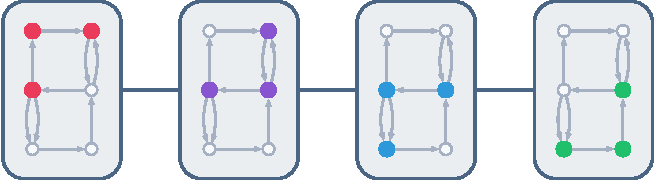
\includegraphics[scale=.65]{fig/semantic-tw/ex-tree-dec-full.pdf}%
	}
	\hfill
	\subfloat[``Concise'' representation of $\tup{\?T, \bagmap}$]{%
		\AP\label{fig:ex-tree-dec-concise}
		\hspace{.5cm}
		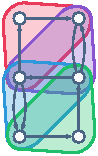
\includegraphics[scale=1.3]{fig/semantic-tw/ex-tree-dec-concise.pdf}
		\hspace{.5cm}
	}
	\hfill
	\caption{
		\AP\label{fig:ex-tree-dec}
		Two different representations of the same "tree decomposition" $\tup{\?T, \bagmap}$ of a 
		"directed graph" $\?G$ with six 
		vertices. The underlying tree is a path with four nodes and each "bag" contains 3 
		vertices---hence the "decomposition@tree decomposition" has "width" 2.
	}
\end{figure}
We give an example of "tree decomposition" in \Cref{fig:ex-tree-dec}:
\begin{itemize}
	\item In \Cref{fig:ex-tree-dec-full}, we give the ``full'' representation of
	the "decomposition@tree decomposition": we draw $\?T$,
	and inside each of the four "bags" $b$ of $\?T$
	we represent a copy of $\?G$. Nodes of $\?G$ belonging to $b$ are highlighted, while the others are dimmed. Sometimes, we will only write the
	name of the nodes contained in the "bag", instead of drawing the graph.
	\item In \Cref{fig:ex-tree-dec-concise}, we give a ``concise'' representation:
	we draw over $\?G$ a coloured shape for each "bag" of $\?T$. This representation is ambiguous---the structure of $\?T$ is not made explicit---and will only be used for
	the most simple cases.
\end{itemize}

The \AP""width"" of a "tree decomposition" $\tup{\?T, \bagmap}$ is the maximum size of a "bag" minus one, "ie" $\max{|\bagmap(b)|-1 \mid b\in T}$.
The \AP""tree-width"" of $\?G$ is the minimum of the "width" of all "tree decompositions" of $\?G$. 
The notion can be directly generalized to arbitrary "relational structures":
instead of asking that every edge $\{u,v\}$ is contained in some "bag",
we required that for every "hyperedge" $\tup{x_1,\dotsc,x_k}$,
there exists a "bag" than contains all $x_i$'s.
The \reintro{tree-width} of a "CQ" is naturally defined as
the "tree-width" of its "canonical database@@cq".
The "undirected graphs" of "tree-width" at most $1$ are exactly
the forests, "ie" the "disjoint unions" of trees.
On the other hand, the "graph@@dir" of \Cref{fig:ex-tree-dec} has "tree-width" $2$.
The "$k$-clique" has "tree-width" exactly $k-1$ since any "tree decomposition"
of $\clique{k}$ must actually contain a "bag" that contains all vertices of $\clique{k}$.

\begin{proposition}[{\cite[Theorem~3]{ChekuriRajaraman2000Containment}}]
	\!\footnote{Theorem 3 talks about query "containment" of "CQs", which is in fact equivalent
	to the "evaluation problem" for "CQs". Moreover, the theorem deals with ``query width'',
	but this parameter is equivalent up to a multiplicative constant to the "tree-width"
	\cite[Lemma~2]{ChekuriRajaraman2000Containment} assuming that the "signature" is fixed.} 
	\footnote{An equivalent result was in fact proven a decade ealier
	by Freuder \cite[Theorem~3]{Freuder1990Complexity} using the
	vocabulary of "constraint satisfaction problems".}
	\AP\label{prop:eval-CQ-bounded-tw}
	For any fixed "signature" $\sigma$,
	for every $k\in\N$, "conjunctive query evaluation" can
	be solved in polynomial time when restricted to "CQs" of
	"tree-width" at most $k$.
\end{proposition}

\Cref{prop:eval-CQ-bounded-tw}, as most algorithms on structures of
bounded "tree-width" actually relies on the ability to compute
a "tree decomposition".
\begin{proposition}[{Bodlaender's algorithm \cite[Theorem~1.1]{Bodlaender1996Treewidth}}]
	\!\footnote{The fact that $k$ is fixed is crucial: if it is also
	part of the input, the problem become "NP"-complete
	\cite[Theorem~3.3]{ArnborgCorneilProskurowski1987Complexity}}
	\label{prop:bodlaender}
	For every \emph{fixed} $k\in\Np$, there is a linear-time algorithm
	which takes as input a "finite structure" and decides
	if it has "tree-width" at most $k$, in which case it also
	outputs a witness of the form of a "tree decomposition" of "width" at most $k$. 
\end{proposition}

\begin{proof}[Proof sketch of {\Cref{prop:eval-CQ-bounded-tw}}]
	We are given as input a "CQ" $\gamma(\bar x)$ of "tree-width" at most $k$,
	and a "pointed relational database" $\tup{\?D,\bar d}$, and need
	to decide if $\tup{\?D, \bar d} \FOmodels \gamma(\bar x)$.
	"Wlog", using Bodlaender's algorithm (\Cref{prop:bodlaender}),
	we assume that we also have a "tree decomposition" $\tup{\?T,\bagmap}$
	of the "canonical database@@cq" $\tup{\?G, \bar x}$ of $\gamma(\bar x)$.

	We do a bottom-up algorithm on the tree $\?T$,
	which maintains a set $\+H$ of partial "homomorphisms" from
	$\tup{\?G, \bar x}$ to $\tup{\?D, \bar d}$.
	In light of \Cref{fig:ex-tree-dec-full}, the idea is to compute
	for each "bag" where the variables it contains could be mapped
	on the databases.
	Formally, we want this procedure
	to satisfy the following invariant:
	when dealing with "bag" $b$, a partial "homomorphism"
	$f\colon \tup{\?G, \bar x} \pto \tup{\?D, \bar d}$ belongs to $\+H_b$ if, and only if,
	\begin{itemize}
		\item the domain of $f$ is $\bagmap(b)$, and
		\item $f$ can be extended into a partial "homomorphism"
			$\tilde f\colon \tup{\?G, \bar x} \pto \tup{\?D, \bar d}$
			defined exactly on the union of $\bagmap(b')$ where $b'$ ranges
			over vertices that are bellow $b$ in the tree $\?T$.
	\end{itemize}
	For leaves $b$, the procedure is easy: we enumerate every possible map
	from $\bagmap(b)$ to $\?D$, and only keep those that define a 
	partial "homomorphism" $\tup{\?G, \bar x} \pto \tup{\?D, \bar d}$: this
	yields a set $\+H_b$ of partial "homomorphisms".
	Then, when dealing with a node $b$ whose children are $b_1,\hdots,b_k$,
	again we enumerate every possible map $f$
	from $\bagmap(b)$ to $\?D$, but then only keep those that
	(1) define a partial "homomorphism" $\tup{\?G, \bar x} \pto \tup{\?D, \bar d}$,
	and (2) agree with the children "bags", in the sense that there must exist
	partial "homomorphisms" $f_1 \in \+H_{b_1}$, $\dotsc$, $f_k \in \+H_{b_k}$
	"st" $f$ and $f_i$ agree on their common vertices,
	"ie" $\restr{f}{\bagmap(b)\cap \bagmap(b_i)} = \restr{f_i}{\bagmap(b)\cap \bagmap(b_i)}$
	for all $i \in \lBrack 1,k\rBrack$.
	
	The correctness of this procedure follows from the assumption that,
	in a "tree decomposition", the set of "bags" "containing@@bag" any node
	must be a connected subset: in some sense this is what allows us to make
	consistent choices.
	Then, to decide if $\tup{\?D, \bar d} \FOmodels \gamma(\bar x)$,
	we check if the set of partial "homomorphisms" associated to the root
	is non-empty. If so, since every vertex must appear in some "bag",
	the invariant yields the existence of a "homomorphism" 
	from $\tup{\?G, \bar x}$ to $\tup{\?D, \bar d}$.
	Otherwise, there is no such "homomorphism". Correctness follows by "duality@@CQ".

	Lastly, concerning the complexity, observe that the "tree decomposition"
	has "width" at most $k$, so there at most
	$|D|^{k+1}$ maps from any fixed "bag" to $\?D$: we can enumerate them all
	in polynomial time since $k$ is fixed! 
	To compute the partial "homomorphisms" $f$ that agree with
	some partial "homomorphisms" from $\+H_{b_1}$, $\dotsc$, $\+H_{b_k}$,
	we can first sort each table $\+H_{b_i}$ according to their value on $\bagmap(b)$,
	and then use a dichotomy search. Sorting can be done
	in $\+O(|D|^{k+1}\log(|D|^{k+1})) = \+O(|D|^{k+1}\log(|D|))$,
	and the dichotomy search---one for each partial "homomorphisms" that is a candidate
	for $\+H_b$---runs in $\+O(\log(|D|^{k+1})) = \+O(\log(|D|))$.
	Overall, we get an algorithm that runs in time
	\[
		\+O(|T|\cdot |D|^{k+1}) = \+O(|\vars{\gamma}|\cdot |D|^{k+1}),
	\]
	up to logarithmic factors.
\end{proof}

Note also that, given a "tree decomposition" of a "structure" $\?A$,
and a "substructure" $\?B$ of $\?A$, by intersecting each "bag" with $B$,
we obtain a "tree decomposition" of $\?B$. It follows that the "tree-width"
of a "substructure" is always upper bounded by the "tree-width" of the full "structure".
In other words, "conjunctive queries" of "tree-width" at most $k\in\N$
form a "monotone class of CQs".

Grohe, Schwentick and Segoufin proved that there
are no graph property other than "tree-width" that ensures
polynomial time evaluation 
\cite[Corollary~19]{GroheSchwentickSegoufin2001Evaluation}.%
Importantly, this statement deals with \emph{graph properties},
"ie" with classes of CQs defined by restricting their underlying "structure".
We will see next that actually there are other classes of CQs
with tractable evaluation.

\paragraph*{Bounded Semantic Tree-Width.}
As mentioned in \Cref{sec:intro-existential}, \Cref{prop:eval-CQ-bounded-tw}
together with the notion of "core" actually yields a tractability result
for a larger class of queries than those of bounded tree-width.

\begin{proposition}
	For any $k\in\N$, the "CQ evaluation problem",
	restricted to "conjunctive queries" that are "semantically equivalent" 
	to a "CQ" of "tree-width" at most $k$ is "fixed-parameter tractable"
	when parametrized by the size of the query.
\end{proposition}

\begin{proof}
	The algorithm goes as follows:
	we start by computing the "core@@CQ" $\coreCQ\gamma(\bar x)$
	of the "CQ" $\gamma(\bar x)$, and then instead of evaluating
	$\gamma(\bar x)$ on the "database@@rel", we instead evaluate
	$\coreCQ\gamma(\bar x)$, using the polynomial-time algorithm
	of \Cref{prop:eval-CQ-bounded-tw}.
	Overall, the algorithm runs in time
	\[
		\+O(f(\size{\gamma})\cdot|\vars{\gamma}|\cdot |D|^{k+1}),
	\]
	up to logarithmic factors, and where $f(\size{\gamma})$
	is the time required to compute the "core@@CQ" of
	$\gamma$.\footnote{This can be done in exponential time.}
	Hence, the problem is "FPT" when parametrized by $\size{\gamma}$.
\end{proof}

In fact, Dalmau, Kolaitis and Vardi improved this result: in a surprising twist, 
one does not need to explicitly the "core" to efficiently evaluate
a "CQ" that is "semantically equivalent" to one of small "tree-width".
They proved that this class could actually be evaluated in polynomial time
\cite[Corollary~5]{DalmauKolaitisVardi2002Constraint}.
Remarkably, Grohe then proved the converse implication: these 
are the only classes of CQs that are tractable!
\begin{proposition}[""Grohe's theorem"" {\cite[Theorem~1.1]{Grohe2007ComplexityHomomorphism}}]
	Let $\sigma$ be a fixed "signature".
	Assuming that "W[1]" $\neq$ "FPT", for any recursively enumerable
	class of "CQs" over $\sigma$, the following are equivalent:
	\begin{enumerate}
		\item there exists $k\in\N$ "st" the "tree-width" of the "cores@@cq"
			of the queries in the class is bounded by $k$;
		\item its evaluation problem is "fixed-parameter tractable"
			when parametrized by the size of the query;
		\item its evaluation problem can be solved in polynomial time.
	\end{enumerate}
\end{proposition}

\begin{marginfigure}
	\centering
	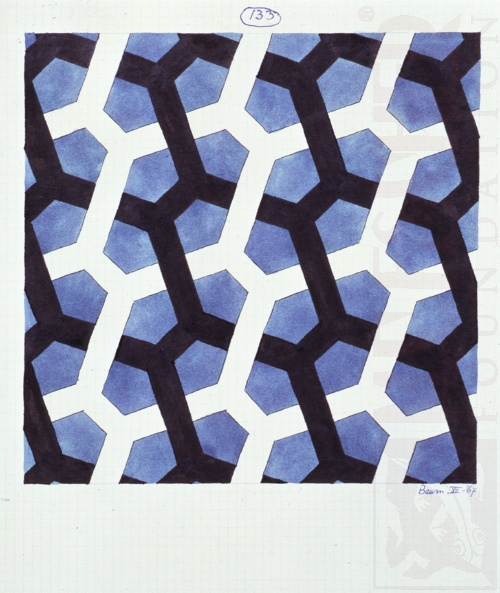
\includegraphics[width=\linewidth]{fig/escher/e133.jpg}
	\caption{\href{https://mcescher.com/gallery/watercolor/\#iLightbox[gallery\_image_1]/3}{\emph{E~133}}, M. C. Escher, \textcopyright~The M.C. Escher Company.}
\end{marginfigure}
The difficult implication in this theorem is (3) $\Rightarrow$ (1).
Grohe proves it by contraposition, by generalizing
the ideas of \cite{GroheSchwentickSegoufin2001Evaluation}:
in short, given a class whose "cores" have unbounded "tree-width",
using the Excluded Minor Theorem \cite[$\ast$ (1.5)]{RobertsonSeymour1986GraphMinors5}
one can find an query in the class whose "core" 
contains an arbitrarily large grid. In turn, the clique problem,
which is "W[1]"-hard, is then reduced to the evaluation problem
for these queries with big grids.

"Grohe's theorem" deals with fixed "signatures": it was later generalized \cite[Theorem~1]{ChenGottlobLanzingerPichler2020Semantic} for characterizing "FPT" "evaluation" when the "signature" is also part. This is done by replacing the notion of "tree-width" with 
that of ``submodular width'', introduced by Marx in \cite{Marx13Tractable}.

\paragraph{Bounded Path-Width.}
We now focus on "path-width", which is a parameter upper-bounded
by the "tree-width".
So, if a "class of CQs" has bounded "path-width", then
it has bounded "tree-width" and so by \Cref{prop:eval-CQ-bounded-tw}
it can be evaluated in polynomial time.
We shall see that "CQs" of small "path-width"
can in fact be evaluated even more efficiently, namely in "NL"!
We define a \AP""path decomposition"" to be a "tree decomposition" $\tup{\?T,\bagmap}$
in which $\?T$ is a path, such as in \Cref{fig:ex-tree-dec}.
The \AP""path-width"" of a "structure" is the minimum of the "width" of
all of its "path decompositions".

\begin{lemma}[{\cite[Lemma~8.10]{FigueiraMorvan2025SemanticTreeWidthLMCS}}]
	\!\footnote[][5em]{\cite[Lemma~8.10]{FigueiraMorvan2025SemanticTreeWidthLMCS},
	corresponding to \Cref{lemma:evaluation-bounded-pathwidth} in this thesis,
	actually proved this result over the larger class of "UC2RPQs" of bounded 
	"path-width". The proof of the upper bound is exactly the same,
	but the lowerbound is \emph{marginally} harder.}
	\AP\label{lemma:evaluation-bounded-pathwidth-cq}
	For each $k \geq 1$, the "CQ evaluation problem", restricted to "CQs" of
	"path-width" at most $k$, is "NL"-complete.
\end{lemma}

\begin{figure*}[tb]
	\centering
	\subfloat[Partial homomorphism computed at the fourth step of the algorithm.]{
		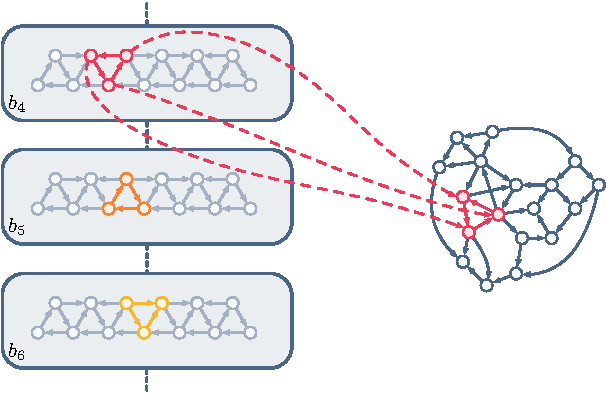
\includegraphics[width=.45\linewidth]{fig/semantic-tw/eval-pw-nl-1.pdf}
	}
	\hfill
	\subfloat[Partial homomorphism computed at the fifth step of the algorithm.]{
		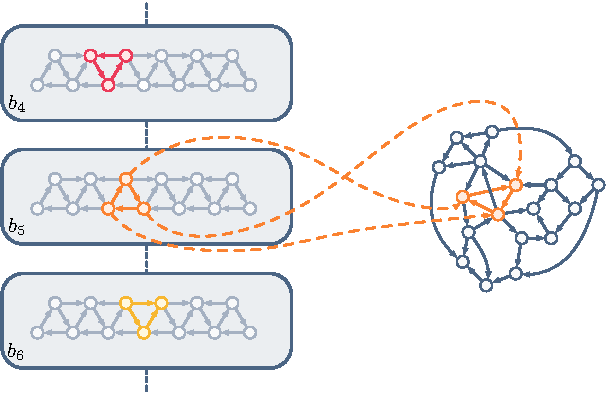
\includegraphics[width=.45\linewidth]{fig/semantic-tw/eval-pw-nl-2.pdf}
	}
	\caption{
		\AP\label{fig:eval-pw-nl}
		Algorithm to evaluate a "CQ" of "path-width" at most $k$ (here $k=2$)
		in "NL". Each subfigure represents a "path decomposition" of the "CQ"
		(on the left-hand side) and a "relational database" (on the right-hand side),
		together with a partial "homomorphism" from the first to the second.
	}
\end{figure*}

\begin{proof}
	\proofcase{Lower bound.}
	We reduce the problem of "Reachability in finite graphs"
	"NL"-hardness directly follows from the "NL"-hardness of
	the "reachability problem in finite graphs".
	Given an instance $\tup{\?G,s,t}$ of this problem,
	we reduce it to
	\[
		\tup{\?G', s, t} \FOmodels^?
		\rho(x_1,x_n) \defeq x_1 \to x_2 \land x_2 \to x_3 \land \dotsc \land x_{n-1} \to x_n,
	\]
	where $n = |G|$ and $\?G'$ is the "graph@@dir" obtained
	from $\?G$ by adding a self-loop on $t$.
	Clearly, there is a path from $s$ to $t$
	in $\?G$ "iff" there is a path from $s$ to $t$ of length at most $n$ in $\?G$---by pigeon-hole principle---, which in turn is equivalent to asking for a path from $s$ to $t$
	of length \emph{exactly} $n$ in $\?G'$ thanks to the extra self-loop.
	To conclude, note that $\rho$ has "path-width" one.

	\proofcase{Upper bound, first part: with the "path decomposition".}
	First, we assume that a "path decomposition" of width at most $k$ of the query of
	is also provided as part of the input. Moreover, we assume "wlog" that the input is "C2RPQ"---the extension to "UC2RPQ" being straightforward. So, we are given as input:
	\begin{itemize}
		\item a "database@@relpointed" $\tup{\?D, \bar d}$,
		\item a "CQ" $\gamma(\bar x)$, and
		\item a "path decomposition" $\langle T, \bagmap \rangle$ of "width" at 	
			most $k$ of $\gamma(\bar x)$.
	\end{itemize}
	The algorithm, illustrated in \Cref{fig:eval-pw-nl}, maintains a partial "homomorphism"
	$f\colon \?G \pto \?D$.
	We scan the "bags" of the decomposition from top to bottom.
	\begin{itemize}
		\item Initially---before even scanning the first "bag"---$f$ is the map with empty domain.
		\item Then, when scanning the $i$-th bag $b_i$,
			we start by restricting $f$ to variables of $\dom(f)\cap \bagmap(b_i)$.
			Then, we extend $f$ so that it is defined on the whole "bag" $\bagmap(b_i)$.
			For every variable $y$ in $\bagmap(b_i) \smallsetminus\dom(f)$:
			\begin{itemize}
				\item if it belongs to $\bar x$, say $y = x_i$, 
					we let $f(x_i) \defeq u_i$;
				\item otherwise, we non-deterministically guess the value of $f(y)$.
			\end{itemize}
			We then check, for every "atom" $\+R_{(k)}(x_1,\hdots,x_k)$ of $\gamma(\bar x)$ 
			"st" all $x_j$'s occur in $\bagmap(b_i)$ if
			$\tup{f(x_1), \dotsc, f(x_k)} \in \+R_{(k)}(\?D)$.
			If not, we reject. 
	\end{itemize}
	If the algorithm manages to scan the whole bag decomposition without rejecting, it accepts.

	Completeness of the algorithm is trivial. Correctness follows from the fact that if
	a variable occurs in "bags" $b_i$ and $b_k$ with $i \leq k$, then it must also belong to every
	"bag" $b_j$ for $j \in \intInt{i,k}$. As a consequence, a variable $x$ is assigned 
	exactly one value $f(x)$ during the whole process. 

	Concerning the space complexity,
	by construction, at the $i$-th step of the algorithm, $f$ is defined exactly on $b_i$, so on at most $k+1$ variables.
	And so, $f$ can be stored in space $(k+1)\log(|D|)$.
	We also need a counter with $\log(|T|)$ bits to scan through the "path decomposition".
	Overall, the algorithm runs in non-deterministic space
	$\+O(k\log(|D|) + \log(|T|)) = \+O(\log(|D|) + \log(|T|))$,
	which is logarithmic in the size of the input.

	\proofcase{Upper bound, second part: without the "path decomposition".}
	Then, we claim that the original problem---when the "tree decomposition" is not part of 
	the input---also lies in "NL". This is because one can compute, from $\gamma$, a
	"path decomposition" in (deterministic) logarithmic space by\footnote{This result is an 
	adaption of a similar statement for "tree-width" \cite[Theorem I.1, p. 143]{ElberfeldJakobyTantau2010Logspace}. Note that the promise that the query has bounded "path-width"---in fact bounded "tree-width" suffices---in a crucial assumption of  \cite[Theorem I.1, p. 143]{ElberfeldJakobyTantau2010Logspace}.} 
	\cite[Theorem 1.3, p. 2]{KintaliMunteanu2010Computing}.
	The conclusion follows since functions computable in non-deterministic logarithmic space
	are closed under composition \cite[Lemma 4.17, p. 88]{AroraBarak2009ComputationalComplexity}. 
\end{proof}

\subsection{Unions of Conjunctive Queries}
\label{sec:prelim-db-ucq}

\begin{marginfigure}
	\centering
	\directlua{width = 2.3; height = 1.4}
\input{tikz/prelim-databases/abstract-lattice.lua}%do not indent!!!
	\begin{tikzpicture}[every node/.style={inner sep=0pt,outer sep=0pt},font=\footnotesize]
		\directlua{draw_lattice()}
		\begin{scope}
\begin{luacode}
			make_clip()
			x = -1.25
			y = -.2
			d1 = .5
			d2 = .75
			d3 = .9
			d4 = .85
			h = height ; w = width ; s = h/w
			colour = "cBlue"
			tex.print(string.format("\\begin{scope}[xshift=%f cm, yshift=%f cm]", x, y+height))
			tex.print(string.format("\\draw[draw=%s, fill=%s, fill opacity=.4] (0,%f) -- (%f,%f) -- (%f, %f) -- (%f,%f) -- (%f,%f) -- (%f,%f) -- (%f,%f) -- (%f,%f) -- (%f, 0) -- cycle;", colour, colour, -height, d1, -h+d1*s, d1+d2, -h+(d1-d2)*s, d1+d2+d3, -h+(d1-d2+d3)*s, d1+d2+d3+d4, -h+(d1-d2+d3-d4)*s, d1+d2+d3+d4+w, (d1-d2+d3-d4)*s, d1+d2+d3+d4+w, h, -w, h, -width))
			-- tex.print(string.format("\\node[circle, fill=%s, minimum size=4pt, outer sep=1pt] at (0,%f) {};", colour, -height))
			tex.print("\\end{scope}")
\end{luacode}
		\end{scope}
	\end{tikzpicture}
	\caption{
		\AP\label{fig:ex-ucq} Semantics of a "union of conjunctive queries" (in blue)
		in the distributive lattice of "relational databases".
	}
\end{marginfigure}
\begin{marginfigure}
	\centering
	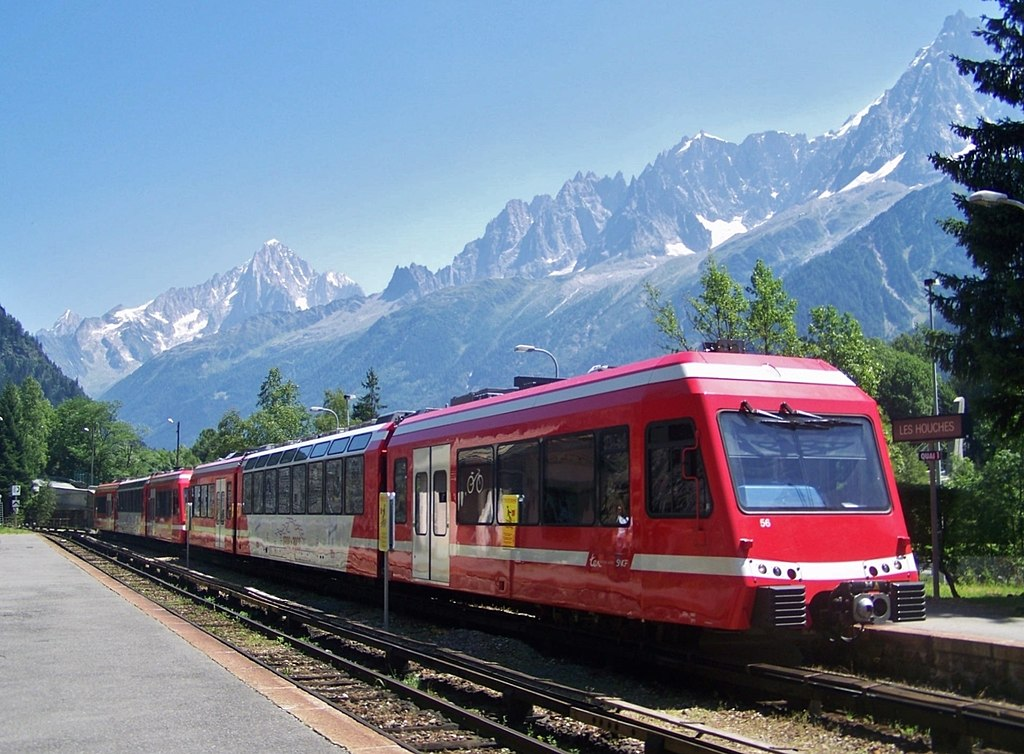
\includegraphics[width=\linewidth]{fig/prelim-db/Houches.jpg}
	\caption{
		The study of (co-)"UCQs" is intriguingly popular amongst finite model theorists. 
		\href{https://fr.m.wikipedia.org/wiki/Fichier:TER\_en\_gare\_des\_Houches\_(Haute-Savoie).JPG}{\emph{TER en Gare des Houches}}, by Florian Pépellin,
		licensed under "CC BY SA 3.0".
	}
\end{marginfigure}
We now show that the desirable properties of "conjunctive queries" can be
lifted to finite unions of such queries.
As mentioned in \Cref{sec:prelim-db-poset-cq}, "conjunctive queries"
are not closed under semantical union: for instance,
the query ``the "database@@rel" contains either an $a$-edge or a $b$-edge''
cannot be expressed by a "conjunctive query".
In fact, our graphical depiction of the distributive lattice of "relational databases"
precisely helps us understand this.

Formally, we define a ""union of conjunctive queries"", or \reintro{UCQ} for short,
as a finite set of "conjunctive queries" that all have the same number
of "output variables". This set is denoted disjunctively.
Its semantics is defined as the union of the semantics of the "conjunctive queries" it contains.%
\footnote[][2em]{Strictly speaking it is not necessary
to assume that these "output variables" are equal, however we can assume "wlog" that
it is the case, by $\alpha$-renaming.}
For instance, if $\gamma(x) = x \atom{a} y$ outputs all vertices
with an outgoing $a$-edge and $\delta(x') = x' \atom{b} y' \atom{c} z'$
outputs all vertices with an outgoing $bc$-path, then
$\gamma(x) \lor \delta(x')$ is the "UCQ" asking for all nodes
that are either the source of an $a$-edge or of a $bc$-path.
We denote "UCQs" with capital Greek letters,
and \AP we call ""disjunct"" of $\Gamma$ any "conjunctive query" belonging to a
"UCQ" $\Gamma$.

Notice that "union of conjunctive queries" are also "closed under homomorphisms".
Graphically, we represent them as… unions of "conjunctive queries":
instead of being diamond-shaped, "UCQs" will hence be depicted
as inverted mountain ranges, see \Cref{fig:ex-ucq}.
By the proof of \Cref{prop:codd-thm}, we can notice that "union of conjunctive queries"
are as expressive as "existential-positive formulas", "ie" "first-order formulas"
built out of $\exists$, $\land$ and $\lor$.

\begin{proposition}
	Let $\Gamma$ be a "UCQ". The following are equivalent:
	\begin{enumerate}
		\item $\Gamma$ is "semantically equivalent" to a "conjunctive query";
		\item the semantics of $\Gamma$ contains a unique "hom-minimal" element;
		\item some "disjunct" of $\Gamma$ "contains" all "disjuncts";
		\item $\Gamma$ is "semantically equivalent" to one of its "disjuncts";
		\item $\Gamma$ is "semantically equivalent" to the "weak union" of its "disjuncts";
	\end{enumerate}
\end{proposition}
\begin{figure}
	\centering
	\subfloat[Two "CQs" $\gamma$ and $\delta$ whose semantical union is
		equivalent to a "CQ".]{
\directlua{width = 2.3; height = 1.4}
\input{tikz/prelim-databases/abstract-lattice.lua}%do not indent!!!
	\begin{tikzpicture}[every node/.style={inner sep=0pt,outer sep=0pt},font=\footnotesize]
		\directlua{draw_lattice()}
		\begin{scope}
			\directlua{make_clip()}
			\directlua{draw_cq(.5, -.6, 'c0', 'x')}
			\directlua{draw_cq(.65, .2, 'c2', 'y')}
			\node[below=2pt of x, c0] {$\gamma$};
			\node[below=2pt of y, c2] {$\delta$};
		\end{scope}
	\end{tikzpicture}
	}
	\hfil
	\subfloat[Two "CQs" $\gamma$ and $\delta$ whose semantical union is not
		equivalent to a "CQ". We also represented their "weak union".]{
	\directlua{width = 2.3; height = 1.4}
\input{tikz/prelim-databases/abstract-lattice.lua}%do not indent!!!
	\begin{tikzpicture}[every node/.style={inner sep=0pt,outer sep=0pt},font=\footnotesize]
		\directlua{draw_lattice()}
		\begin{scope}
			\directlua{make_clip()}
			\directlua{draw_cq(.167, -.607, 'cPurple', 'z')}
			\directlua{draw_cq(.5, -.4, 'c0', 'x')}
			\directlua{draw_cq(-.5, -.2, 'c2', 'y')}
			\node[below=2pt of x, c0] {$\gamma$};
			\node[below=2pt of y, c2] {$\delta$};
			\node[below=3.5pt of z, cPurple] {$\gamma \weakunion \delta$};
		\end{scope}
	\end{tikzpicture}
	}
	\caption{
		\label{fig:ucq-equiv-cq} When is a "union of conjunctive queries"
		actually equivalent to a "conjunctive query"?
	}
\end{figure}
 
\begin{proof}
	All the intuitions are provided in \Cref{fig:ucq-equiv-cq}.
	
	\proofcase{(1) $\Rightarrow$ (2).} If $\Gamma$ is "semantically equivalent"
	to a "CQ" $\delta$, then the "canonical database@@cq" $\?D$ of $\delta$ is
	the unique minimal element in the semantics of $\Gamma$.

	\proofcase{(2) $\Rightarrow$ (3).} If the semantics of $\Gamma$
	contains a unique minimal element, say $\?D$, then since $\?D \FOmodels \Gamma$,
	there exists a "disjunct" $\gamma$ of $\Gamma$ "st" $\?D \FOmodels \gamma$.
	By minimality of $\?D$, it follows that $\gamma$ is actually the "canonical CQ" of $\?D$,
	and again by minimality of $\?D$ it follows that all "disjuncts" are "contained" in $\gamma$.

	\proofcase{(3) $\Rightarrow$ (4).} If $\Gamma = \gamma_1 \lor \dotsc \lor \gamma_k$
	has a "disjunct", say $\gamma_i$, that contains all other disjuncts, then
	\[
		\Gamma = \gamma_1 \lor \dotsc \lor \gamma_k \contained
		\gamma_i \lor \dotsc \lor \gamma_i \semequiv \gamma_i \contained \Gamma
	\]
	and so $\Gamma$ is "semantically equivalent" to its "disjunct" $\gamma_i$.

	\proofcase{(4) $\Rightarrow$ (5).} If $\Gamma = \gamma_1 \lor \dotsc \lor \gamma_k$ is "semantically equivalent" to
	one of its disjuncts, say $\gamma_i$, then
	for each $j$ we have $\gamma_j \contained \Gamma \semequiv \gamma_i$,
	and so by definition of the "weak union" as the least upper bound,
	it follows that $\gamma_1 \weakunion \dotsc \weakunion \gamma_k \semequiv \gamma_i$.

	\proofcase{(5) $\Rightarrow$ (1).} If $\Gamma$ is "semantically equivalent" to the
	"weak union" of its "disjuncts", then since this query is a "CQ", it
	is equivalent to a "CQ"…
\end{proof}

\begin{proposition}
	Given two "UCQs" $\Gamma$ and $\Delta$, we have $\Gamma \contained \Delta$
	if, and only if, for every "disjunct" $\gamma \in \Gamma$, there exists
	a "disjunct" $\delta \in \Delta$ "st" $\gamma \contained \delta$.
\end{proposition}

\begin{proof}
	The right-to-left implication is trivial.
	For the converse one, assume that $\Gamma \contained \Delta$,
	and let $\gamma$ be a "disjunct" of $\Gamma$.
	Letting $\?G$ be its "canonical database@@cq", we have by "duality@@CQ" that
	$\?G \FOmodels \Gamma$
	and since $\Gamma \contained \Delta$, it follows that $\?G \FOmodels \Delta$,
	and hence $\?G \FOmodels \delta$ for some "disjunct" $\delta \in \Delta$,
	and so, by "duality@@CQ", $\gamma \contained \delta$. 
\end{proof}

\begin{corollary}
	"Containment" and "semantical equivalence" of "unions of conjunctive queries"
	are "NP"-complete.
\end{corollary}

Essentially, these results are permitted, at least in part, by the fact that semantical union
is well-behaved with respect to "duality@@CQ": this is mostly because their semantics 
is "closed under homomorphisms". Hopefully, one could hope to find larger
query languages satisfying this property, and then deduce decidability results via "duality@@CQ".
Both unfortunately and expectedly, it turns out that there
are no other first-order queries which are "closed under homomorphism".\AP
\begin{proposition}[""Rossman's theorem"", {\cite[Theorem~1.7]{Rossman2008Homomorphism}}]
	\!\footnote{Actually the full statement of the theorem is
	slightly more precise and relates the quantifier-rank of the formulas.
	The original construction was far from optimal, and it was
	recently shown by the same author
	that this rank can actually be preserved by the construction
	\cite[Theorem~1.4]{Rossman2025Equirank}.}%
	\footnote{Both references mention "first-order sentences"; however we do not see
	any reason why it would not apply to all "first-order formulas".}
	The semantics over "finite relational structures"
	of a "first-order sentence" is "closed under homomorphisms"
	if, and only if, it is equivalent to a "union of conjunctive queries".
\end{proposition}

We leave to the reader the care to show that the other properties of "CQs"
can be lifted to "UCQs", for instance:
\begin{itemize}
	\item starting from a "UCQ" $\gamma_1 \lor \dotsc \lor \gamma_k$,
		the "UCQ" obtained by (1) considering the "cores@@CQ"
		$\coreCQ\gamma_1$, $\dotsc$, $\coreCQ\gamma_k$,
		(2) putting aside those that are "contained" in another "core",
		and (3) taking their union
		yields a "UCQ" that is "semantically equivalent" to the
		original one, and minimal under most reasonable metrics;
	\item the evaluation of "UCQs" of bounded "tree-width"---we naturally
		extend the notion of "tree-width" to unions by letting it
		be the maximum of the "tree-width" of its "disjuncts"---is
		polynomial time. 
\end{itemize}
\section{Graph Databases}

\AP ""Graph databases"" are abstracted as edge-labelled directed graphs
$G = \langle \vertex{G}, \edges{G} \rangle$, 
where nodes of $\intro*\vertex{G}$ represent entities and labelled edges $\intro*\edges{G} \subseteq \vertex G \times \A \times \vertex G$
represent relations between these entities, with $\A$ being a fixed finite alphabet.
For instance, \Cref{fig:example-graph-database} depicts a "graph database",
whose nodes are authors and papers, on the alphabet
$\A = \{\text{\color{wrote}wrote},\,\text{\color{advised}advised}\}$.
Edges $x \atom{\wrote} y$ indicate that the person $x$ wrote the paper $y$,
while edges $x \atom{\advised} y$ indicate that person $x$ was
the Ph.D. advisor of person $y$.

\begin{figure}[ht]
    \centering
    \begin{tikzpicture}
        \node (a1) {author$_1$};
        \node (a2) [right = of a1] {author$_2$};
        \node (a3) [right = of a2] {author$_3$};
        \node (a4) [right = of a3] {author$_4$};
        \node (a5) [right = of a4] {author$_5$};
        \node (p1) [below = 2.5em of a2] {paper$_1$};
        \node (p2) [below = 2.5em of a3] {paper$_2$};
        \node (p3) [below = 2.5em of a4] {paper$_3$};

        \draw[wrote] (a1) to[edge, ->] node[fill=white] {\footnotesize wrote} (p1)
            (a2) to[edge, ->] node[fill=white] {\footnotesize wrote} (p1)
            (a2) to[edge, ->] node[fill=white] {\footnotesize wrote} (p2)
            (a3) to[edge, ->] node[fill=white] {\footnotesize wrote} (p2)
            (a4) to[edge, ->] node[fill=white] {\footnotesize wrote} (p3)
            (a5) to[edge, ->] node[fill=white] {\footnotesize wrote} (p3);
        \draw[advised] (a4) to[edge, ->, bend right=60] node[fill=white] {\footnotesize advised} (a3)
            (a5) to[edge, ->, bend right=60] node[fill=white] {\footnotesize advised} (a4);
    \end{tikzpicture}
    \caption{%
        \AP\label{fig:example-graph-database}%
        A "graph database" with eight nodes and eight edges on a two-letter alphabet.
    }
\end{figure}

\AP Being a subclass of relational databases, "graph databases" can be queried by the
predominant query language of ""conjunctive queries"", "aka" "CQs", 
which consists of the closure under projection---"aka" existential quantification---of conjunctions of atoms of the form $x \atom{a} y$
for some letter $a \in \A$. For instance, the "conjunctive query"
\[
    \gamma_1(x, y) = x \atom{\wrote} z
        \land y \atom{\wrote} z    
\]
returns, when "evaluated" on the "graph database" $G$
defined in \Cref{fig:example-graph-database}, all pairs of nodes $(u, v)$ such that $u$ is a co-author
of $v$. Each variable not appearing in the left-hand side of 
the definition of a "conjunctive query" (in this example, $z$) is implicitly 
existentially quantified. 
Note that, to the cost of losing the information of which variable is existentially quantified, every "CQ"
can be seen as a "graph database", where each variable is a node, and each atom is an edge; 
hence, we sometimes use "graph database" terminology for "CQs".

The expressive power of "CQs" is somewhat limited, since
"CQs" cannot express, for example, transitive closure.
Since the ability to navigate paths is of importance in many "graph database" 
scenarios, most modern graph query languages support, as a central querying mechanism,
"conjunctive regular path queries", or "CRPQs" for short. 
In particular, "CRPQs" form the core navigational mechanism of the new ISO standard Graph Query Language (GQL) \cite{ISO2024GQL} and the SQL extension for querying graph-structured data SQL/PGQ \cite{ISO2023PGQ} (see also \cite{FrancisEtal2023GPCIcdt,FrancisEtal2023GPC}).

"CRPQs" are 
defined analogously to "conjunctive queries", except that their atoms are now of the form 
$x \atom{L} y$ where $L$ is an arbitrary regular language over the alphabet $\A$. For 
instance the "evaluation" of the "CRPQ"
\[
    \gamma_2(x, y) = x \atom{\wrote} z
        \land z' \atom{\wrote} z 
        \land y \atom{({\advised})^*} z'
\]
on $G$ yields every pair of persons $(u,v)$ such that $u$ is a co-author of a
``scientific descendant'' of $v$. 

\AP Formally, a ""CRPQ"" $\gamma$ is defined as a tuple $\bar z = (z_1,\hdots,z_n)$
of ""output variables"", "aka" \reintro{free variables},\footnote{For technical reasons (see the definition of "equality atoms") we allow for a variable to appear multiple times.}
together with a conjunction of ""atoms"" of the form
$\bigwedge_{j=1}^m x_j \atom{L_j} y_j$, where each $L_j$ is a regular language and where $m \geq 0$.
The set of all variables occurring in $\gamma$, namely\footnote{We neither assume 
disjointness nor inclusion between $\{z_1,\hdots,z_n\}$ and $\{x_1,y_1,\hdots,x_m,y_m\}$}
$\{z_1,\hdots,z_n\}\cup\{x_1,y_1,\hdots,x_m,y_m\}$, is denoted by
$\intro*\vars(\gamma)$.
Given a "database@@graph" $G$, we say that a tuple of nodes $\bar u = (u_1,\hdots,u_n)$
\AP""satisfies@@db"" $\gamma$ 
on $G$ if there is a mapping
$\fun\colon \vars(\gamma) \to \vertex{G}$ such that $u_i = \fun(z_i)$ for all
$1 \leq i \leq n$, and for each $1 \leq j \leq m$,
there exists a path from $\fun(x_i)$ to $\fun(y_i)$ in $G$, labelled by
a word from $L_i$ (if the path is empty, the label is $\epsilon$). The \AP""evaluation"" of $\gamma$ on $G$ is then the set of all tuples that "satisfy@@db" $\gamma$.
%
For example, $(\text{author}_2, \text{author}_5)$ "satisfies@@db" $\gamma_2$ 
on the "graph database" $G$ of \Cref{fig:example-graph-database} via
the function that maps $x$ to $\text{author}_2$, $y$ to $\text{author}_5$,
$z$ to $\text{paper}_2$, and $z'$ to $\text{author}_3$.

\AP
The language of "CRPQ" can be extended to navigate edges in both directions. 
\knowledgenewrobustcmd{\Gpm}{\cmdkl{G^\pm}}
Consider the expanded database $\intro*\Gpm$ obtained from $G$ by 
% keeping the same vertices, copying the edges of $G$, and 
adding, for every edge $x \atom{a} y$ in $G$, an extra edge $y \atom{a^-} x$.
We obtain a graph database on the alphabet $\intro*\Aext = \A \cup \A^-$ where
$\A^- = \set{a^- \mid a \in \A}$. We then define the syntax of
a \AP""CRPQ with two-way navigation"", or \reintro{C2RPQ}, as a "CRPQ" on the alphabet $\Aext$.
Its \reintro{evaluation} is defined as the "evaluation" of the "CRPQ" on $\Gpm$.
For instance, the "evaluation" of the "C2RPQ"
\[
    \gamma_3(x, y) = x \atom{({\wrote}\cdot{\wrote}^-)^*} y
\]
on the "graph database" of \Cref{fig:example-graph-database} returns all pairs of
individuals linked by a chain of co-authorship.
It includes $(\text{author}_1, \text{author}_3)$ or $(\text{author}_1, \text{author}_1)$
but not $(\text{author}_1, \text{author}_4)$.
%
\AP If a query has no "output variables" we call it ""Boolean"", and
its "evaluation" can either be the set $\set{()}$, in which case we say that $G$
\reintro(db){satisfies} the query, or the empty set $\set{}$. For example, $G$ "satisfies@@db" the
"Boolean CRPQ"
\[\gamma_4() = x \atom{\wrote} y\]
if, and only if, the database contains one author together with one paper they wrote.

We denote the set of "atoms" of a "C2RPQ" $\gamma$ by \AP$\intro*\atoms\gamma$, and by 
$\intro*\nbatoms{\gamma}$ we denote its number of "atoms", "ie", $|\atoms\gamma|$.
Moreover, we denote by $\intro*\size{\gamma}$ the sum of its number of "atoms" with
the sum of the size of NFAs used to describe $\gamma$.

\AP Finally, a ""union of CQs"" (\reintro{UCQs}) (resp.\ ""union of CRPQs"" (\reintro{UCRPQs}), resp.\ ""union of C2RPQs"" (\reintro{UC2RPQs}))  
is defined as a finite set of "CQs" (resp.\ "CRPQs", resp.\ "C2RPQs"), whose
tuples of "output variables" have all the same arity. 
\AP
A ""subquery"" of a "C2RPQ" $\gamma$ is any "C2RPQ" resulting from removing some "atoms" (possibly none) from $\gamma$. A \reintro{subquery} of  "UC2RPQ" is a union of "subqueries" of the "C2RPQs" therein.
The "evaluation" of a union is defined as the union of its "evaluations", for instance the following "UCQ"
\begin{align*}
    \Gamma_5 & = \gamma_{5}^1(x, y) \lor \gamma_{5}^2(x, y) \\
    & \text{ where }
    \gamma_{5}^1(x, y) = x \atom{\wrote} y %\\
    \text{ and }
    \gamma_{5}^2(x, y) = x \coatom{\advised} z \land
        z \atom{\wrote} y
\end{align*}
"evaluates" to the set of pairs $(x,y)$ such that $y$ is a paper written by either $x$
or their advisor.
We naturally extend the notations $\nbatoms{-}$ and $\size{-}$ to "unions@UC2RPQs".
\AP ""Infinitary unions"" are defined analogously, except
that we allow for potentially infinite unions. We often use a set notation to denote the union, especially for "infinitary unions".

For a more detailed introduction to "CRPQs", we refer the reader to \cite{Figueira2020Containment21Foundations}.
For a more general introduction to different query languages for "graph databases"---including "CRPQs"---see \cite{Barcelo2013Querying}, and for a more practical approach,
see \cite{AnglesEtal2017Foundations}.

\smallskip

% \paragraph*{Containement and equivalence}
\AP %It is often interesting to compare queries together. 
The ""evaluation problem"" for "UC2RPQ" is the problem of, given
a "UC2RPQ" $\Gamma$, a "graph database" $G$ and a tuple $\bar u$ of elements of $G$,
whether $\bar u$ "satisfies@@db" $\Gamma$ on $G$. 
Given two "UC2RPQ" $\Gamma$
and $\Gamma'$ whose "output variables" have the same arity,
we say that $\Gamma$ is \AP""contained"" in $\Gamma'$,
denoted by $\Gamma \intro*\contained \Gamma'$ if
for every "graph database" $G$, for every tuple $\bar u$ of $G$,
if $\bar u$ "satisfies@@db" $\Gamma$ on $G$, then so does $\Gamma'$ (we will hence reserve the symbol `$\subseteq$' for set inclusion---note in particular that inclusion (of the "UC2RPQs", seen as sets of "C2RPQs") implies "containment", but the converse does not hold). 
The \AP""containment problem"" for "UC2RPQs" is the problem of, given
two "UC2RPQs" $\Gamma$ and $\Gamma'$, to decide if $\Gamma \contained \Gamma'$.
When $\Gamma$ is "contained" in $\Gamma'$ and vice versa, we say that
$\Gamma$ and $\Gamma'$ are \AP""semantically equivalent"", denoted by
$\Gamma \intro*\semequiv \Gamma'$. 

\begin{itemize}
	\itemAP $\intro*\Exp$ and ""expansion""
	\itemAP $\intro*\cdb$ and ""canonical database""
	\itemAP $\intro*\Refin$, ""atom refinement"", ""refinement""
	\itemAP $\intro*\contract{L_i \cdots L_{j}}$, ""one-way contraction"", ""contraction"" and ""condensation"" -> unify terminology; ""contracting internal variables"", ""internal path""
	\itemAP $\intro*\nbatoms{\gamma}$, $\intro*\nbvar{\gamma}$
	\itemAP ""evaluation map""
	\itemAP ""simple regular expression"" and ""positive simple regular expression""
\end{itemize}

A \AP""class of (Boolean) CRPQs"" is a function \AP$\intro*\classCRPQ$ mapping an alphabet $\A$ 
to a set $\classCRPQ_{\A}$ of "Boolean CRPQs", which is closed under variable renaming and alphabetic
renaming of the languages.

\subsection{Small tree-width}


It is known that the "evaluation problem" for "UC2RPQ" is "NP"-complete, just as for "conjunctive queries"
\cite[Theorem 7]{ChandraMerlin1977Implementation}.
However, queries whose underlying structure looks like a tree---formally, queries of bounded 
"tree-width"---can be "evaluated" in polynomial time \cite[Theorem 3]{ChekuriRajaraman2000Containment}.\footnote{Theorem 3 talks about query "containment" of "CQs", which is in fact equivalent to the "evaluation problem" for "CQs". Moreover, the theorem deals with ``query width'', but this parameter is equivalent up to a multiplicative constant to the "tree-width" \cite[Lemma 2]{ChekuriRajaraman2000Containment} assuming that the database signature arity is fixed.} 

\AP
"Tree-width" is a measure of how much a
graph differs from a tree, introduced by Arnborg, Corneil and
Proskurowski~\cite{ArnborgCorneilProskurowski1987Complexity}.
% who noticed that many "NP"-complete problems become polynomial-time solvable on classes of graphs of bounded tree-width \cite{ArnborgCorneilProskurowski1987Complexity}.
%
For a gentle but thorough introduction to "tree-width", we refer the reader to
\cite[\S 3.6]{NesetrilPOM2012Prolegomena}. Formally, a \AP""tree decomposition"" of a multigraph $G$ is a
pair $(T, \intro*\bagmap)$ where $T$ is a tree and $\bagmap: \vertex{T} \to \pset{\vars(G)}$ is a function that associates to each node of $T$, called \AP""bag"",
a set of vertices of $G$. When $x \in \bagmap(b)$ we shall say that the "bag"
$b \in \vertex{T}$ \AP""contains@@tw"" vertex $v$. Further, it must satisfy the following three properties:
\begin{itemize}
    \item each vertex $v$ of $\gamma$ is "contained@@tw" in at least one "bag" of $T$;
    \item for each edge $u \atom{} v$ of $G$, there is at least one "bag" of $T$
        that "contains@@tw" both $u$ and $v$; and 
    \item for each vertex $v$ of $G$, the set of bags of $T$ "containing@@tw" $v$ is a 
        connected subset of $\vertex{T}$.
\end{itemize}
The \AP""width"" of $(T, \bagmap)$ is the maximum of $|\bagmap(b)|-1$ when $b$ ranges over
$\vertex{T}$.

\begin{figure}
	\centering
	\subfloat[``Full'' representation of $(T, \bagmap)$.]{%
		\AP\label{fig:ex-tree-dec-full}
		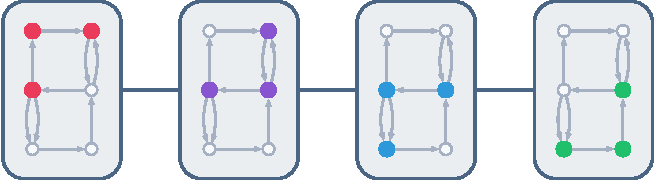
\includegraphics[scale=.5]{fig/semantic-tw/ex-tree-dec-full.pdf}%
	}
	\hfill
	\subfloat[``Concise'' representation of $(T, \bagmap)$]{%
		\AP\label{fig:ex-tree-dec-concise}
		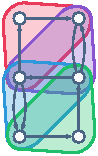
\includegraphics[scale=1.1]{fig/semantic-tw/ex-tree-dec-concise.pdf}
	}
	\caption{
		\AP\label{fig:ex-tree-dec}
		Two different representations of the same "tree decomposition" $(T, \bagmap)$ of a 
		multigraph $G$ with six 
		vertices. The underlying tree is a path with four nodes and each "bag" contains 3 
		vertices---hence the "decomposition@tree decomposition" has "width" 2.
	}
\end{figure}
We give an example of "tree decomposition" in \Cref{fig:ex-tree-dec}:
\begin{itemize}
	\item In \Cref{fig:ex-tree-dec-full}, we give the ``full'' representation of
	the "decomposition@tree decomposition": we draw $T$, and inside each "bag" $b$ of $T$
	we represent a copy of $G$. Nodes of $G$ belonging to $b$ are highlighted, while the others are dimmed. Sometimes, we will only write the
	name of the nodes contained in the "bag", instead of drawing the graph.
	\item In \Cref{fig:ex-tree-dec-concise}, we give a ``concise'' representation:
	we draw over $G$ a coloured shape for each "bag" of $T$. This representation is ambiguous---the structure of $T$ is not made explicit---and will only be used when no ambiguity can arise.
\end{itemize}

The \AP""tree-width"" of $G$ is the minimum of the "width" of all "tree decompositions" of $G$. The \reintro{tree-width} of a "C2RPQ" is the "tree-width" of its underlying multigraph. 
We denote by $\intro*\Tw$ (resp.\ $\intro*\TwOneWay$) the set of all "C2RPQs" (resp.\ "CRPQs") of "tree-width" at most $k$. The \reintro{tree-width} of a "UC2RPQ" is simply the maximum of the "tree-width" of its "C2RPQs".
\AP
A ""path decomposition"" is a "tree decomposition" $(T,\bagmap)$ in which $T$ is a path. The \AP""path-width"" of $\gamma$ is the minimum of the "width" among all "path decompositions" of $\gamma$. The \reintro{path-width} of a "C2RPQ" and "UC2RPQ" are defined analogously. We denote by \AP$\intro*\Pw$ (resp.\ $\intro*\PwOneWay$) the set of all "C2RPQs" (resp.\ "CRPQs") of "path-width" at most $k$. The relationship between these classes is depicted in \Cref{fig:taxonomy-syntactic}:
note that $\TwOneWay$ and $\PwOneWay$ are not explicitly drawn, but correspond to the
intersection of $\Tw$ (resp.\ $\Pw$) with the class of "CRPQs".

\begin{figure}
	\centering
	\scalebox{1.125}{
	\begin{tikzpicture}
		\node at (0,0) {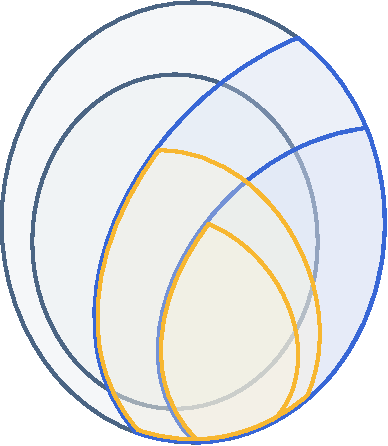
\includegraphics[scale=.8]{fig/semantic-tw/taxonomy-syntactic.pdf}};
		% \draw[line width=1.5pt] (0,-4) -- (0,4);
		% \draw[line width=1.5pt] (-3,0) -- (3,0);
		% \draw[line width=.5pt] (1,-4) -- (1,4);
		% \draw[line width=.5pt] (-3,1) -- (3,1);
		% \draw[line width=.5pt] (-1,-4) -- (-1,4);
		% \draw[line width=.5pt] (-3,-1) -- (3,-1);
		\node[font=\small] at (.5,-1.5)
			{$\withkl{\kl[\Pw]}{\cmdkl{\color{cYellow}\mathcal{P\hspace{-.15em}w}_{1\!}}}$};
		\node[font=\small] at (-.5,0) 
			{$\withkl{\kl[\Pw]}{\cmdkl{\color{cYellow}\mathcal{P\hspace{-.15em}w}_{k\!}}}$};
		\node[font=\small] at (2.05,.2)
			{$\withkl{\kl[\Tw]}{\cmdkl{\color{cBlue}\mathcal{T\hspace{-.15em}w}_{1\!}}}$};
		\node[font=\small] at (1.4,1.8)
			{$\withkl{\kl[\Tw]}{\cmdkl{\color{cBlue}\mathcal{T\hspace{-.15em}w}_{k\!}}}$};
		\node[font=\tiny] at (-1.5,.5) {\kl[CRPQ]{\color{cDarkGrey}CRPQs}};
		\node[font=\tiny] at (-.5,2.4) {\kl[C2RPQ]{\color{cDarkGrey}C2RPQs}};
	\end{tikzpicture}
	}
	\caption{
		\AP\label{fig:taxonomy-syntactic}
		Clickable taxonomy of syntactic classes defined using "tree-width".
	}
\end{figure}


Similar statements of the following proposition can be considered Folklore (see "eg" {\cite[Theorem IV.3]{RomeroBarceloVardi2017Homomorphism}}); however, our inability to find a proof for it with sharp bounds invites us to include a proof.
\begin{restatable}[Proof in \Cref{apdx-sec:prop:crpq-bound-tree-width-upper-bound}]{proposition}{crpqboundtwupperbound}
	\AP\label{prop:crpq-bound-tree-width-upper-bound}
    For each $k \geq 1$, the "evaluation problem" for "UC2RPQs" of "tree-width" at
    most $k$ can be solved in time $\+O(\size{\Gamma} \cdot |G|^{k+1} \cdot \log{|G|})$ on a Turing machine,
	or $\+O(\size{\Gamma} \cdot |G|^{k+1})$ under a RAM model, where $\Gamma$ and $G$ are the input "UC2RPQ" and "graph database", respectively.
\end{restatable}

In practice, "graph databases" tend to be huge and often changing, while queries
are in comparison very small.
This motivates the following question, given some natural $k \geq 1$: 

\begin{center}
    \AP 
    Given a "UC2RPQ" $\Gamma$, is it "equivalent" to a "UC2RPQ" $\Gamma'$ of "tree-width" at most $k$?\\
    That is, does it have ""semantic tree-width"" at most $k$?
\end{center}
This problem is called the ""semantic tree-width $k$ problem"".
Should it be decidable in a constructive way---that is, decidable, and if the answer is positive, we can compute a witnessing $\Gamma'$ from $\Gamma$---, then one could, once and for all,
compute $\Gamma'$ from $\Gamma$ and, whenever one wants to "evaluate" $\Gamma$ on a
database, "evaluate" $\Gamma'$ instead.

We will also study the restriction of these notions to one-way queries: a "UCRPQ" has \AP""one-way semantic tree-width"" at most $k$ if it is equivalent to a "UCRPQ" of "tree-width" at most $k$. The \AP""one-way semantic tree-width $k$ problem"" is the problem of, given a "UCRPQ" $\Gamma$, whether it has "one-way semantic tree-width" at most $k$.

\begin{example}
    \AP\label{ex:CRPQ-tw3-stw2}
    Consider the following "CRPQs",\footnote{In this graphical representation,
	we interpret a labelled graph as the "CRPQ" defined as
	the conjunction of the "atoms" induced by the labelled edges of the graph.
	For instance, $\gamma(\bar x)$ is a conjunction of six "atoms".}
    where $\bar x = (x_0,x_1,y,z)$:\leavevmode
    \begin{center}
        \small
        \begin{tikzcd}[column sep=small, row sep=small]
            &[-.5em] x_0 \ar[dr, "a"] \ar[rr, "c"] \ar[ddr, "a(bb)^+" swap, pos=.6, bend right] & &
            x_1 \ar[dl, "a" swap] \ar[ddl, "ab(bb)^*", pos=.7, bend left]
                &[1.5em] &[-.5em] x_0 \ar[dr, "a"] \ar[rr, "c"] \ar[ddr, "a(bb)^+" swap, pos=.6, bend right] & &
                x_1 \ar[dl, "a" swap] 
                    &[1.5em] &[-.5em] x_0 \ar[dr, "a"] \ar[rr, "c"]  & &
                    x_1 \ar[dl, "a" swap] \ar[ddl, "ab(bb)^*", pos=.6, bend left] \\
            \gamma(\bar x) \defeq & & y \ar[d, "b^+", pos=.35] & 
                & \delta(\bar x) \defeq & & y \ar[d, "b(bb)^*" pos=.35] & 
                    & \delta'(\bar x) \defeq & & y \ar[d, "(bb)^+" swap, pos=.35] & \\
            & & z & 
                & & & z & 
                    & & & z &
        \end{tikzcd}
    \end{center}
    \noindent
    The underlying graph of $\gamma(\bar x)$ being the directed 4-clique, $\gamma 
    (\bar x)$ has "tree-width" 3. We claim that $\gamma(\bar x)$ is equivalent to the "UCRPQ"
    $\delta(\bar x) \lor \delta'(\bar x)$, and hence has "one-way semantic tree-width" at most 2.

    Indeed, given a "graph database" satisfying $\gamma(\bar x)$ via some mapping $\mu$, 
    it suffices to make a case disjunction on whether the number of $b$-labelled "atoms"
    in the path from
    $\mu(y)$ to $\mu(z)$ is even or odd. In the first case, the "atom" $x_0\atom{a(bb)^+} z$ becomes
    redundant since we can deduce the existence of such a path from the conjunction
    $x \atom{a} y \atom{(bb)^+} z$, and hence the "database@@graph" "satisfies@@db" $\delta(\bar x)$ via $\mu$.
    Symmetrically, in the second case, the "atom" $x_1 \atom{b(bb)^*} z$ becomes redundant,
    and the "database@@graph" "satisfies@@db" $\delta'(\bar x)$ via $\mu$. 
    Thus, $\gamma(\bar x)$
    is "contained", and hence "equivalent" (the other "containment" being trivial), to
    the "UCRPQ" $\delta(\bar x) \lor \delta'(\bar x)$ of "tree-width" 2.
\end{example}

\subsection{\AP{}Related Work}
\label{sec:relwork}
On the class "conjunctive queries", the "semantic tree-width $k$ problem" becomes the "coNP"-complete problem of finding out whether the retraction of a query has "tree-width"
at most $k$. In fact, "CQs" enjoy the effective existence of unique minimal queries \cite[Theorem 12]{ChandraMerlin1977Implementation}, which happen to also minimize the tree-width. For "CRPQs" and "UC2RPQs", the question is far more challenging, and it has only been solved for the case $k = 1$ 
by Barceló, Romero, and Vardi \cite[Theorem 6.1]{BarceloRomeroVardi2016SemanticAcyclicity}; the case $k>1$ was left widely open
\cite[\S 7]{BarceloRomeroVardi2016SemanticAcyclicity}.

Furthermore, classes of "CQs" of bounded "semantic tree-width" precisely characterize tractable (and "FPT") "evaluation problem" \cite[Theorem~1.1]{Grohe2007ComplexityHomomorphism}.
This result is on bounded-arity schemas, which was later generalized \cite[Theorem~1]{ChenGottlobLanzingerPichler2020Semantic} for characterizing "FPT" "evaluation" on arbitrary schemas---by replacing "semantic tree-width" with semantic ``submodular width'' \cite{Marx13Tractable}.

The problem of computing "maximal under-approximations" of "CQs" of a given "tree-width" has been explored in \cite{BarceloLibkinRomero2014Efficient}.
A "maximal under-approximations" of tree-width at most $k$ of a "CQ" $\gamma$ consists of a
"CQ" $\delta_k$ of "tree-width" at most $k$, which under-approximates it,
"ie" $\delta_k$ is "contained" in $\gamma$, and which is maximal, in the sense that for every "CQ" 
$\delta'$, if $\delta'$ has "tree-width" at most $k$ and is "contained" in $\gamma$, then 
$\delta'$ is "contained" in $\delta_k$. 
"Maximal under-approximations" of a given "tree-width" for "CQs" always exist \cite{BarceloLibkinRomero2014Efficient} and thus, a "CQ" is "semantically equivalent"
to a "CQ" of "tree-width" at most $k$ if, and only if, it is equivalent to its maximal under-approximation of "tree-width" at most $k$. Our solution to decide the
"semantic tree-width $k$ problem" for "UC2RPQs" is based on this idea.

While "maximal under-approximations" always exist for "CQs", this is not the case for the dual notion of ``minimal over-approximations''. The problem of when these exist is still unknown to be decidable, aside for some the special cases of acyclic "CQs" and Boolean "CQs" over binary schemas \cite{BarceloRomeroZeume2020Approximation}.

% % ---
% % Minimization paper
% % ---

% \paragraph{Graph databases.}
% \AP ""Graph databases"" are abstracted as edge-labelled directed graphs
% $G = \langle \vertex{G}, \edges{G} \rangle$, 
% where nodes of $\intro*\vertex{G}$ represent entities and labelled edges $\intro*\edges{G} \subseteq \vertex G \times \A \times \vertex G$
% represent relations between these entities, with $\A$ being a fixed finite alphabet.

% \paragraph{Conjunctive regular path queries (CRPQs) and unions of CRPQs (UCRPQs).}
% \AP A ""CRPQ"" $\gamma$ is defined as a tuple $\bar z = (z_1,\hdots,z_n)$
% of ""output variables""\footnote{For technical reasons (see the definition of "equality atoms") we allow for a variable to appear multiple times.},
% together with a conjunction of ""atoms"" of the form
% \AP$\bigwedge_{j=1}^m x_j \intro*\atom{L_j} y_j$, where each $L_j$ is a regular language
% and where $m \geq 0$.
% The set of all variables occurring in $\gamma$, namely%
% \footnote{We neither assume 
% disjointness nor inclusion between $\{z_1,\hdots,z_n\}$ and $\{x_1,y_1,\hdots,x_m,y_m\}$.}
% $\{z_1,\hdots,z_n\}\cup\{x_1,y_1,\hdots,x_m,y_m\}$, is denoted by
% $\intro*\vars(\gamma)$. Variables in $\vars(\gamma)\setminus \{z_1,\hdots,z_n\}$ are existentially quantified. 
% We denote by $\intro*\atoms(\gamma)$ the set of "atoms" of $\gamma$.
% Given a "database@@graph" $G$, we say that a tuple of nodes $\bar u = (u_1,\hdots,u_n)$
% \AP""satisfies@@db"" $\gamma$ 
% on $G$ if there is a mapping
% $\fun\colon \vars(\gamma) \to \vertex{G}$ such that $u_i = \fun(z_i)$ for all
% $1 \leq i \leq n$, and for each $1 \leq j \leq m$,
% there exists a (directed) path from $\fun(x_j)$ to $\fun(y_j)$ in $G$, labelled by
% a word from $L_j$ (if the path is empty, the label is $\varepsilon$). The \AP""evaluation"" of $\gamma$ on $G$ is then the set of all tuples that "satisfy@@db" $\gamma$ on $G$.

% A ""union of CRPQs"" (\reintro{UCRPQs})
% is defined as a finite set of "CRPQs", called \AP""disjuncts"", whose tuples of "output variables" have all the same arity.
% The "evaluation" of a union is defined as the union of its "evaluations". 
% If a query has no "output variables" we call it ""Boolean"", and
% its "evaluation" can either be the set $\set{()}$, in which case we say that $G$
% \reintro(db){satisfies} the query, or the empty set $\set{}$.

% \AP Given two "UCRPQs" $\Gamma$
% and $\Gamma'$ whose "output variables" have the same arity,
% we say that $\Gamma$ is \AP""contained"" in $\Gamma'$,
% denoted by $\Gamma \intro*\contained \Gamma'$, if
% for every "graph database" $G$, for every tuple $\bar u$ of $\vertex{G}$,
% if $\bar u$ "satisfies@@db" $\Gamma$ on $G$, then so does $\Gamma'$. We will hence reserve the symbol `$\subseteq$' for set inclusion.
% The \AP""containment problem"" for "UCRPQs" is the problem of, given
% two "UCRPQs" $\Gamma$ and $\Gamma'$, to decide if $\Gamma \contained \Gamma'$.
% When $\Gamma \contained \Gamma'$ and $\Gamma' \contained \Gamma$  we say that
% $\Gamma$ and $\Gamma'$ are \AP""equivalent"", denoted by
% $\Gamma \intro*\semequiv \Gamma'$. 

% \AP A ""conjunctive query"" (\reintro{CQ}) is in this context a "CRPQ" whose every atom is of the form $x \atom{a} y$ for $a \in \A$ ("ie", every language is a singleton $\set{a}$).
% \AP A ""union of CQs"" (\reintro{UCQs}) is defined as a "UCRPQ" with the same property.

% A \AP""canonical database"" $G$ of a "CRPQ" $\gamma$ is any "canonical database" associated
% to an "expansion" of $\gamma$, see \cite[Definition 3.1]{FlorescuLevySuciu1998Containment}
% for a formal definition. We denote it by \AP$G \intro*\cdb \gamma$.
% A \reintro{canonical database} of a "UCRPQ" is a "canonical database" of one
% of its "disjuncts".

% An \AP""evaluation map"" from a "CRPQ" $\gamma$ to a "graph database" $G$
% in a function $f$ from variables of $\gamma$ to $G$ "st"
% for any atom $x \atom{L} y$ in $\gamma$, there is path from $f(x)$ to $f(y)$ in $G$
% labelled by a word of $L$.

% The "containment" between "UCRPQs" $\Gamma_1 \contained \Gamma_2$ is exactly characterized
% by the fact that for all "canonical database" $G_1 \cdb \Gamma_1$,
% there exists a "disjunct" $\gamma_2$ of $\Gamma_2$ "st" there is an "evaluation map"
% from $\gamma_2$ to $G_1$.

% \paragraph{Homomorphisms.}
% \AP A ""homomorphism"" $\fun$ from a "CRPQ" $\gamma(x_1, \dotsc, x_m)$ to a "CRPQ" $\gamma'(y_1, \dotsc, y_m)$ is a mapping from $\vars(\gamma)$ to $\vars(\gamma')$ such that $\fun(x) \atom{L} \fun(y)$ is an "atom" of $\gamma'$ for every "atom" $x \atom{L} y$ of $\gamma$, and further $\fun(x_i)=y_i$ for every $i$.
% Such a "homomorphism" $\fun$ is \AP""strong onto"" if for every "atom" $x' \atom{L} y'$ of $\gamma'$ there is an "atom" $x \atom{L} y$ of $\gamma$ such that $\fun(x)=x'$ and $\fun(y)=y'$.
% % An example of "homomorphism" is provided in \Cref{fig:basic-hom}.
% We write $\gamma \intro*\homto \gamma'$ if there is a "homomorphism" from $\gamma$ to $\gamma'$, and $\gamma \intro*\surjto \gamma'$ if there is a "strong onto homomorphism".
% In the latter case, we say that $\gamma'$ is a \AP""homomorphic image"" of $\gamma$.
% A \reintro{homomorphism} $\fun$ from a graph database $G$ to a graph database $G'$ is a mapping from $\vertex{G}$ to $\vertex{G'}$ such that  for every edge $u \atom{a} v$ of $G$, it holds that $\fun(u) \atom{a} \fun(v)$ is an edge in $G'$. A "homomorphism" from a "CQ" to a graph database is defined analogously.  

% \AP It is easy to see that if $\gamma \homto \delta$ then $\delta \contained \gamma$, and in the case where $\gamma,\delta$ are "CQs" this is an ``if and only if'' \cite[Lemma 13]{ChandraMerlin1977Implementation}. 
% \AP Two "CQs" $\gamma,\delta$ are ""hom-equivalent"" if there are "homomorphisms" $\gamma \homto \delta$ and $\delta \homto \gamma$.
% Hence, for any two "CQs" $\gamma, \delta$, we have $\gamma \semequiv \delta$ if, and only if, they are "hom-equivalent".
% \AP The ""core"" of a "CQ" $\gamma$, denoted by $\intro*\core(\gamma)$
% is the result of repeatedly removing any atom which results in an equivalent query. It is unique up to isomorphism (see, "eg", \cite{ChandraMerlin1977Implementation}). We say that a "CQ" is `a core' if it is isomorphic to its "core". If $\gamma$ and $\delta$ are "hom-equivalent" then they have
% the same "core". Moreover, there is always an \AP""embedding""---"ie", a "homomorphism" which is injective both on variables and "atoms"---of $\core(\gamma)$ into $\gamma$.

% \paragraph*{Refinements and expansions of (U)CRPQs.}
% \AP For an NFA $\+A$ and two states $q,q'$ thereof, we denote by $\intro*\subaut{\+A}{q}{q'}$ the ""sublanguage"" of $\+A$ recognized  when considering $\set{q}$ as the set of initial states and $\set{q'}$ as the set of final states.
% \AP An ""atom $m$-refinement"" of a "CRPQ" "atom" $\gamma(x,y) = x \atom{L} y$ where $m\geq 1$ and $L$ is given by the NFA $\+A_L$ is any "CRPQ" of the form 
% \begin{equation}
% 	\AP\label{eq:refinement}
% 	\rho(x,y) = x \atom{L_1} t_1 \atom{L_2} \hdots \atom{L_{n-1}} t_{n-1} \atom{L_n} y
% \end{equation}
% where $1 \leq n \leq m$, $t_1,\hdots,t_{n-1}$ are fresh (existentially quantified) variables,
% and $L_1,\hdots,L_n$ are such that there exists a sequence $(q_0,\dotsc,q_n)$ of states of $\+A_L$
% such that $q_0$ is initial, $q_n$ is final, and for each $i$, $L_i$ is either of the form
% \begin{enumerate}[label=\roman*.]
% 	\item $\subaut{\+A_L}{q_{i-1}}{q_{i}}$, or 
% 	\item $\{a\}$ if the letter $a\in \A$ belongs to $\subaut{\+A_L}{q_{i-1}}{q_{i}}$.
% \end{enumerate}
% Additionally, if $\varepsilon \in L$, the \AP""equality atom"" ``$x = y$'' is also an \reintro{atom $m$-refinement}. Thus, an \reintro{atom $m$-refinement} can be either of the form \eqref{eq:refinement} or ``$x=y$''.
% By definition, note that the concatenation
% $L_1\cdots L_n$ is a subset of  $L$ and hence $\rho \contained \gamma$ for any "atom $m$-refinement" $\rho$ of $\gamma$.
% An \AP""atom refinement"" is an "atom $m$-refinement" for some $m$.

% Given a natural number $m$, an \AP""$m$-refinement"" of a "CRPQ" $\gamma(\bar x) = \bigwedge_{i} x_i \atom{L_i} y_i$ is any query resulting from: (1) replacing every "atom" by one of its "$m$-refinements@@atom", and (2)
% should some "$m$-refinements@@atom" have "equality atoms",
% collapsing the variables (and removing the identity atoms `$x=x$').
% \AP A ""refinement"" is an "$m$-refinement" for some $m$.
% Note that in a "refinement" of a "CRPQ"
% the "atom refinements" need not have the same length.
% For instance, both $\rho(x,x) = x \atom{c} x$ and $\rho'(x,y) = x \atom{a} t_1 \atom{a} y \coatom{c} y$ are "refinements" of $\gamma(x,y) = x \atom{a^*} y \coatom{c} x$.
% \AP
% We write $\intro*\Refin(\gamma(\bar x))$ to denote the set of all "refinements" of $\gamma(\bar x)$ and $\reintro*\Refin[\leq m](\gamma(\bar x))$ to the $m$-refinements. 

% The set of \AP""expansions"" of a "CRPQ" $\gamma$ is the set $\intro*\Exp(\gamma)$ of all "CQs" which are "refinements" of $\gamma$.
% In other words, an "expansion" of $\gamma$ is any "CQ" obtained from $\gamma$
% by replacing each "atom" $x \atom{L} y$ by a path $x \atom{w} y$ for some
% word $w \in L$. The "expansions" (resp.\ "refinements") of a "UCRPQ" are the "expansions" (resp.\ "refinements") of the "CRPQs" it contains.
% We define \AP""atom expansions"" analogously to "atom refinements". For "UCRPQs" we use  $\Exp(\Gamma)$, $\Refin(\Gamma)$ and $\Refin[\leq m](\Gamma)$ as for "CRPQs".

% Any "UCRPQ" is equivalent to the infinitary union of its "expansions". In light of this, 
% the semantics for "UCRPQs" can be rephrased as follows. 
% Given a "UCRPQ" $\Gamma(\bar x)$ and a graph database $G$, 
% the "evaluation" of $\Gamma(\bar x)$ on $G$, denoted by $\Gamma(G)$, is the set of tuples 
% $\bar{v}$ of nodes for which there is $\anexpansion \in \Exp(\Gamma)$ such that there is a "homomorphism" $\anexpansion \homto G$ that sends $\bar x$ onto $\bar v$. 

% "Containment" of "UCRPQs" can also be characterized in terms of "expansions".
% \begin{proposition}[Folklore, see e.g. {\cite[Proposition 3.2]{FlorescuLevySuciu1998Containment}} or
% 	{\cite[Theorem 2]{CalvaneseDeGiacomoLenzeriniVardi2000Containment}}]
% 	\AP\label{prop:cont-char-exp-st} 
% 	Let $\Gamma_1$ and $\Gamma_2$ be "UCRPQs". Then the following are equivalent:
% 	% \begin{itemize}
% 		% \item 
% 		(i) $\Gamma_1 \contained \Gamma_2$;
% 		% \item 
% 		(ii) for every $\anexpansion_1\in \Exp(\Gamma_1)$, $\anexpansion_1 \contained \Gamma_2$;
% 		% \item 
% 		(iii) for every $\anexpansion_1\in \Exp(\Gamma_1)$ there is $\anexpansion_2\in \Exp(\Gamma_2)$ such that $\anexpansion_2\homto \anexpansion_1$. 
% 	% \end{itemize}
% \end{proposition}

% \begin{hypothesis}
% 	To simplify proofs, we often assume that the regular languages are described via non-deterministic finite automata (NFA) instead of regular expressions,
% 	which does not affect any of our complexity bounds.
% 	However, for readability all our examples will be given in terms of regular expressions.
% \end{hypothesis}

% \AP We denote by $\intro*\nbatoms{\gamma}$ the number of "atoms" of a "CRPQ" $\gamma$ and by $\intro*\nbvar{\gamma}$ the number of variables.
% We extend these notations to a "UCRPQ" $\Gamma$ by letting
% $\nbatoms{\Gamma} = \max_{\gamma \in \Gamma} \nbatoms{\gamma}$
% and $\nbvar{\Gamma} = \max_{\gamma \in \Gamma} \nbvar{\gamma}$. 
% We denote by $\size{\Gamma}$ the size (of a reasonable encoding) of a  "UCRPQ". 
% For a CRPQ $\gamma$, we define its  \AP""underlying graph"" $\intro*\underlying{\gamma}$ of $\gamma$ as the directed multigraph obtained from $\gamma$ by ignoring the regular languages labelling the atoms of $\gamma$. 

% We assume familiarity with basic concepts of directed multigraphs.
% For simplicity, thorough the paper, by `graph' we mean a directed multigraph. We also adapt implicitly in the natural way, concepts defined for "CRPQs" to (directed multi)graphs (such a "homomorphisms", "embeddings", etc.).

% Formally, a \AP""contraction@@var"" of an "internal variable" $y$ in a "CRPQ" $\gamma$ is the result of replacing any pair of distinct atoms $x \atom{L} y$ and $y \atom{L'} z$ with $x \atom{L \cdot L'} z$ for $L \cdot L' \defeq \set{w \cdot w' : w \in L, w' \in L'}$.%
% \footnote{Note that "contraction of internal variable" is a particular case of "edge contraction".} Observe that this results in an "equivalent" query.
% A \AP""contraction"" of $\gamma$ is any "CRPQ" obtained by repeatedly "contracting@@var" "internal variables".

% % ---
% % Semantic tree-width
% % ---

% Before attacking the statement of our "Key Lemma" in \Cref{sec:maximal-under-approximations},
% we first give a few elementary definitions on "C2RPQs" in this section.
% %
% % \paragraph*{Homomorphisms}
% \AP
% A homomorphism $\fun$ from a "C2RPQ" $\gamma(x_1, \dotsc, x_m)$ to a "C2RPQ" $\gamma'(y_1, \dotsc, y_m)$ is a mapping from $\vars(\gamma)$ to $\vars(\gamma')$ such that $\fun(x) \atom{L} \fun(y)$ is an "atom" of $\gamma'$ for every "atom" $x \atom{L} y$ of $\gamma$, and further $\fun(x_i)=y_i$ for every $i$.
% Such a "homomorphism" $\fun$ is \AP""strong onto"" if for every "atom" $x' \atom{L} y'$ of $\gamma'$ there is an "atom" $x \atom{L} y$ of $\gamma$ such that $\fun(x)=x'$ and $\fun(y)=y'$.
% An example of "homomorphism" is provided in \Cref{fig:basic-hom}.
% We write $\gamma \homto \gamma'$ if there is a "homomorphism" from $\gamma$ to $\gamma'$, and $\gamma \surj \gamma'$ if there is a "strong onto homomorphism".
% \todo{change this shit}
% In the latter case, we say that $\gamma'$ is a \AP""homomorphic image"" of $\gamma$.
% It is easy to see that if $\gamma \homto \gamma'$ then $\gamma' \contained \gamma$, and in the case where $\gamma,\gamma'$ are "CQs" this is an ``if and only if'' \cite[Lemma~13]{ChandraMerlin1977Implementation}.

% \paragraph*{Some intuitions on maximal under-approximations}
% Given a "conjunctive query" $\gamma$,
% the union of all "conjunctive queries"
% that are "contained" in $\gamma$ is "semantically equivalent" to the union
% $\bigvee \{ \gamma' \mid \gamma \surj \gamma' \}$. Naturally, this statement borders on the trivial since $\gamma'$ belongs to this union. It becomes interesting when we add a restriction:
% given a class $\class$ of "CQs" (to which $\gamma$ may not belong) closed under "subqueries", then $\Gamma' \defeq \bigvee \{ \gamma' \in \class \mid \gamma \surj \gamma' \}$ is the maximal under-approximations
% of $\gamma$ by finite unions of "conjunctive queries" of $\class$, in the following sense:
% \begin{enumerate}[label=\roman*.]
% 	\item (finite) $\Gamma'$ is a finite union of "CQs" of $\class$,
% 	\item (under-approximation) $\Gamma' \contained \gamma$, and
% 	\item (maximality) for any finite union $\Delta$ of "CQs" of $\class$, if $\Delta \contained \gamma$, then $\Delta \contained \Gamma'$.
% \end{enumerate}

% \begin{proof}
% Only the last point is non-trivial, and follows from the fact that if
% $\Delta \contained \gamma$, then for each $\delta \in \Delta$, $\delta \contained \gamma$,
% so there is a "homomorphism" $f\colon \gamma \to \delta$. The image $\delta'$
% of $f$ is a "subquery" of $\delta$, and $\+C$ is closed under "subqueries",
% so it belongs to $\+C$, and hence to $\Gamma'$. Since there is a trivial homomorphism
% from $\delta'$ to $\delta$, we moreover have that $\delta \contained \delta'$.
% Hence, for each "CQ" $\delta \in \Delta$, there is a CQ $\delta' \in \Gamma'$ such
% that $\delta \contained \delta'$, and hence $\Delta \contained \Gamma'$.
% \end{proof}

% As a consequence, we deduce that for each $k \geq 1$,
% the "maximal under-approximation" of a "CQ" by
% a finite union of "CQs" of "tree-width" at most $k$ is computable, and hence
% we can effectively decide if some "CQ" is "equivalent" to a query of "tree-width" at
% most $k$ by testing the equivalence with this maximal under-approximation.
% For more details on approximations of "CQs", see \cite{BarceloLibkinRomero2014Efficient}.
% Note that interestingly, changing $\Gamma'$ from
% $\bigvee \{ \gamma' \in \class \mid \gamma \surj \gamma' \}$
% to $\bigvee \{ \gamma' \in \class \mid \gamma' \contained \gamma \}$
% preserves both under-approximation and maximality, but $\Gamma'$ is now an infinite
% union of "CQs" of $\+C$.

% Unfortunately, these results cannot be straightforwardly extended to "conjunctive regular
% path queries" since the previous proof implicitly relied on two points:
% \begin{enumerate}
% 	\item the equivalence between the
% 	"containment" $\gamma' \contained \gamma$ and the existence of a "homomorphism"
% 	$\gamma \homto \gamma'$, and
% 	\item the possibility to restrict $\gamma'$ to its image $\gamma \homto \gamma'$ while 
% 	obtaining a semantically bigger query.
% \end{enumerate}
% These two crucial ingredients is what allows us to build a finite set $\Gamma'$ from $\gamma$.
% For "CRPQs", the second point still holds, but not the first one.
% For instance, the "CQ" $\gamma(x,y) = x \atom{a} z \atom{b} y$ is
% contained in (in fact "equivalent" to) the "CRPQ" $\gamma'(x,y) = x \atom{ab} y$,
% but there is no "homomorphism" from $\gamma'(x,y)$ to $\gamma(x,y)$.
% Our main result shows that to find "maximal under-approximations" of "C2RPQs",
% it suffices to take "homomorphic images" of so-called ``"refinements"'' of $\gamma$,
% instead of "homomorphic images" of $\gamma$ itself. The next paragraphs are devoted to
% introducing "refinements" and tools related to them.

% \paragraph*{Equality Atoms}
% \AP"C2RPQs" with ""equality atoms"" are queries of the form $\gamma(\bar{x}) = \delta \land I$, 
% where $\delta$ is a "C2RPQ" (without equality atoms) and $I$ is a conjunction of "equality atoms" of the form $x=y$. 
% Again, we denote by $\vars(\gamma)$ the set of variables appearing in the (equality and non-equality) atoms of $\gamma$. 
% We define the binary relation $=_\gamma$ over $\vars(\gamma)$ to be the reflexive-symmetric-transitive closure of the binary relation $\{(x, y) \mid \text{$x=y$ is an "equality atom" in $\gamma$}\}$. 
% In other words, we have $x=_\gamma y$ if the equality $x=y$ is forced by the "equality atoms" of $\gamma$. 
% Note that every "C2RPQ" with "equality atoms" $\gamma(\bar{x}) = \delta \land I$ is equivalent to a "C2RPQ" without "equality atoms"  $\gamma^{\collapse}$, 
% which is obtained from $\gamma$ by collapsing each equivalence class of the relation $=_\gamma$ into a single variable. 
% This transformation gives us a \emph{canonical} renaming from $\vars(\gamma)$ to $\vars(\gamma^{\collapse})$. For instance, $\gamma(x,y) \defeq x \atom{K} y \land y \atom{L} z \land x = y$
% collapses to $\gamma^{\collapse}(x,x) \defeq x \atom{K} x \land x \atom{L} z$.

% \paragraph*{Refinements}
% \AP An ""atom $m$-refinement"" of a "C2RPQ" "atom" $\gamma(x,y) = x \atom{L} y$ where $L$ is given by the NFA $\+A_L$ is any "C2RPQ" of the form 
% \begin{equation}
%     \AP\label{eq:refinement}
%     \rho(x,y) = x \atom{L_1} t_1 \atom{L_2} \hdots \atom{L_{n-1}} t_{n-1} \atom{L_n} y
% \end{equation}
% where $1 \leq n \leq m$, $t_1,\hdots,t_{n-1}$ are fresh (existentially quantified) variables,
% and $L_1,\hdots,L_n$ are such that there exists a sequence $(q_0,\dotsc,q_n)$ of states of $\+A_L$
% such that $q_0$ is initial, $q_n$ is final, and for each $i$, $L_i$ is either of the form
% \begin{enumerate}[label=\roman*.]
% 	\item $\subaut{\+A_L}{q_i}{q_{i+1}}$,
% 	\item $\{a\}$ if the letter $a\in \A$ belongs to $\subaut{\+A_L}{q_i}{q_{i+1}}$, or 
% 	\item $\{a^{-}\}$ if $a^{-} \in \A^{-}$ belongs to $\subaut{\+A}{q_i}{q_{i+1}}$.
% \end{enumerate}
% Additionally, if $\epsilon \in L$, the "equality atom" ``$x = y$'' is also an \reintro{atom $m$-refinement}. Thus, an \reintro{atom $m$-refinement} can be either of the form \eqref{eq:refinement} or ``$x=y$''.
% By convention, $t \atom{a^{-}} t'$ is a shorthand for $t' \atom{a} t$. As a consequence,
% the underlying graph of an "atom $m$-refinement" of the form \eqref{eq:refinement} is not necessarily a directed path.
% By definition, note that
% $L_1\cdots L_n \subseteq L$ and hence $\rho \contained \gamma$ for any "atom $m$-refinement" $\rho$ of $\gamma$.
% An \AP""atom refinement"" is an "atom $m$-refinement" for some $m$.
% An example is provided in \Cref{fig:basic-refinement}.

% \begin{marginfigure}
% 	\centering
% 	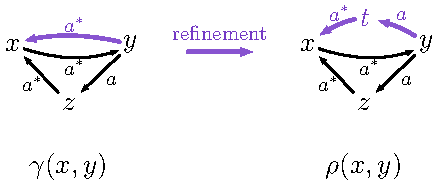
\includegraphics[width=\linewidth]{basic-refinement.pdf}
% 	\caption{\AP\label{fig:basic-refinement}A "refinement".}
% \end{marginfigure}
	
% \begin{marginfigure}
% 	\centering
% 	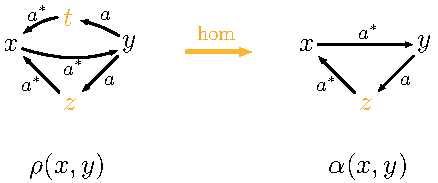
\includegraphics[width=\linewidth]{basic-hom.pdf}
% 	\caption{\AP\label{fig:basic-hom}A "strong onto homomorphism".}
% \end{marginfigure}

% \begin{definition}
%     \AP\label{def:atom-contraction}
%     \AP Given an "atom refinement" $\rho = x \atom{L_1} t_1 \atom{L_2} \hdots \atom{L_{n-1}} t_{n-1} \atom{L_n} y$ of $\gamma = x \atom{L} y$ as in \eqref{eq:refinement}, define
%     a ""condensation"" of $\rho$ between $t_i$ and $t_j$, where $0 \leq i,j \leq n$ and $j > i+1$, as any "C2RPQ" of the form:
%     \[
%         \rho' = x \atom{L_1} t_1 \atom{L_2} \hdots \atom{L_i} \textcolor{cPurple}{t_i \atom{K} t_j} \atom{L_{j+1}} \hdots
%         \atom{L_{n-1}} t_{n-1} \atom{L_n} y
%     \]
%     such that $\textcolor{cPurple}{K = \+A[q_i,q_j]}$.
% 	\begin{fact}
% 		\AP\label{fact:refinement-contained}
% 		Every "condensation" $\rho'$ of $\rho$ is a "refinement" of $\gamma$, and $\rho \contained \rho' \contained \gamma$.
% 	\end{fact}
%     \AP Informally, we will abuse the notation and
%     write $\intro*\contract{L_{i}\cdots L_{j}}$ to denote the language $K$---even if this language
%     does not only depend on $L_{i}\cdots L_{j}$.
% \end{definition}

% \begin{example}
%     \AP\label{ex:atom-refinement-twoway}
%     Let $\gamma(x,y) = x \atom{(aa^-)^*} y$ be a "C2RPQ" "atom", where
%     $(aa^-)^*$ is implicitly represented by its minimal automaton.
%     Then $\rho(x,y)$ is a "refinement" of "refinement length" seven of $\gamma(x,y)$
%     and $\rho'(x,y)$ is a "condensation" of $\rho(x,y)$, where:
%     \begin{align*}
%         \rho(x,y) & = x \atom{a} t_1 \atom{(a^-a)^*} t_2 \atom{(a^-a)^*} t_3
%             \coatom{a} t_4 \atom{(aa^-)^*} t_5 \atom{(aa^-)^*a} t_6 \coatom{a} y, \\
%         \rho'(x,y) & = x \atom{a} t_1 \atom{(a^-a)^*} t_2 \atom{(a^-a)^*} t_3
% 		\coatom{a} t_4 \atom{(aa^-)^*} y. 
%     \end{align*}
%     On the other hand, $\rho''(x,y) = x \atom{a} t_1 \coatom{a} y$ is not
%     a "condensation" of $\rho(x,y)$.
% \end{example}

% Given a natural number $m$, an \AP""$m$-refinement"" of a "C2RPQ" $\gamma(\bar x) = \bigwedge_{i} x_i \atom{L_i} y_i$ is any query resulting from: 1) replacing every "atom" by one of its "$m$-refinements@@atom", and 2)
% should some "$m$-refinements@@atom" have "equality atoms",
% collapsing the variables.
% \AP A ""refinement"" is an "$m$-refinement" for some $m$.
% Note that any "atom $m$-refinements" is, by definition, also an
% "atom $m'$-refinements" when $m \leq m'$: as a consequence, in the "refinement" of a "C2RPQ"
% the "atom refinements" need not have the same length.
% For instance, both $\rho(x,x) = x \atom{c} x$ and $\rho'(x,y) = x \atom{a} t_1 \atom{a} y \coatom{c} y$ are "refinements" of $\gamma(x,y) = x \atom{a^*} y \coatom{c} x$.

% %%%%%%%%%%%%%%%%%%%%%
% %     We will assume that a query "refinement" does not contain atoms with the language $\set{\epsilon}$; these are eliminated by identifying variables in a standard way. For example, if the result of replacing atoms by "atom refinements" yields $\gamma(x,z) = x \atom{\set{\epsilon}} y \land y \atom{\set{\epsilon}} z \land z \atom{a^*} x$ the associated "refinement" is then $\gamma(x,x) =  x \atom{a^*} x$.
% % \sidediego{CHECK}
% %%%%%%%%%%%%%%%%%%%%%
% For a given "C2RPQ" $\gamma$, let $\AP\intro*\Refin[\leq m](\gamma)$ be the set of all "$m$-refinements" of $\gamma$, and $\reintro*\Refin(\gamma)$ be the set of all its "refinements".
% Given a "refinement" $\rho(\bar x)$ of $\gamma(\bar x)$,
% its ""refinement length"" is the least natural number
% $m$ such that $\rho(\bar x) \in \Refin[\leq m](\gamma)$.
% Note that if the automaton representing a language $L$ has more than one final state, for instance the minimal automaton for $L = a^+ + b^+$,
% then $x \atom{L} y$ is not a "refinement" of itself.
% However, it will always be "equivalent" to a union of refinements: in
% this example, $x \atom{a^+ + b^+} y$ is "equivalent" to the union of
% $x \atom{a^+} y$ and $x \atom{b^+} y$, which are both "refinements"
% of the original "C2RPQ".

% \paragraph*{Expansions}
% %%%%%%%%%%%%%%%%%%%%%
% % \sidediego{CHECK}
% % Observe that a "C2RPQ" $\gamma$ whose every language is of the form $\set{z}$ for $z \in \Aext \dcup \set{\varepsilon}$ is equivalent to a "conjunctive query" $\tilde \gamma$. For example, $\gamma(x,y) = x \atom{\varepsilon} y \land y \atom{\set{a^-}} z$ is equivalent to $\tilde\gamma(y,y) = z \atom{a} y$. 
% Remember that a "C2RPQ" whose languages are
% of the form $\set{a}$ or $\set{a^-}$ for $a \in \A$ is in effect a "CQ".
% The \AP""expansions"" of a "C2RPQ" $\gamma$ is the set $\intro*\Exp(\gamma)$ of all "CQs" which are "refinements" of $\gamma$.
% In other words, an "expansion" of $\gamma$ is any "CQ" obtained from $\gamma$
% by replacing each "atom" $x \atom{L} y$ by a path $x \atom{w} y$ for some
% word $w \in L$.
% For instance, $\xi(x,y) = x \atom{a} t_1 \coatom{a} t_2 \atom{a} t_3 \coatom{a} y$
% is an "expansion" of $\rho(x,y) = x \atom{(aa^-)^*} y$.
% %%%%%%%%%%%%%%%%%%%%%
% % l228: But, isn't this the notation used on all previous pages?
% % We will henceforth identify a "C2RPQ" atom $x \atom{\set{a}} y$ \resp{$x \atom{\set{a^-}} y$} as simply $x \atom{a} y$ \resp{$x \coatom{a} y$}, and thus we will consider that the class of "CQs" is a syntactic fragment of the class of "C2RPQs".

% Any "C2RPQ" is equivalent to the infinitary union of its "expansions". In light of this, the semantics for "UC2RPQ" can be rephrased as follows. 
% Given a "UC2RPQ" $\Gamma(\bar x)$ and a graph database $G$, 
% the "evaluation" of $\Gamma(\bar x)$ over $G$, denoted by $\Gamma(G)$, is the set of tuples 
% $\bar{v}$ of nodes for which there is $\anexpansion \in \Exp(\Gamma)$ such that there is a "homomorphism" $\anexpansion \homto G$ that sends $\bar x$ onto $\bar v$.  
% Similarly, "containment" of "UC2RPQs" can also be characterized in terms of expansions.

% \begin{proposition}[Folklore, see e.g. {\cite[Proposition 3.2]{FlorescuLevySuciu1998Containment}} or
%     {\cite[Theorem 2]{CalvaneseDeGiacomoLenzeriniVardi2000Containment}}]
%     \AP\label{prop:cont-char-exp-st} 
%     Let $\Gamma_1$ and $\Gamma_2$ be "UC2RPQs". Then the following are equivalent
%     \begin{itemize}
%         \item $\Gamma_1 \contained \Gamma_2$;
%         \item for every $\anexpansion_1\in \Exp(\Gamma_1)$, $\anexpansion_1 \contained \Gamma_2$;
%         \item for every $\anexpansion_1\in \Exp(\Gamma_1)$ there is $\anexpansion_2\in \Exp(\Gamma_2)$ such that $\anexpansion_2\homto \anexpansion_1$. 
%     \end{itemize}
% \end{proposition}

% Note that since an "expansion" of $\gamma$ is also a "refinement" of $\gamma$, it also
% holds that $\gamma$ is "semantically equivalent" to the infinitary union of its "refinements".

% \AP Given a "C2RPQ" $\gamma$, an \AP""internal path"" is a sequence of atoms\footnote{We write
% $x \symatom{\lambda} y$ to mean that there is either an "atom" $x \atom{\lambda} y$
% \textbf{or} an "atom" $x \coatom{\lambda} y$.}
% \[
% 	x_0 \symatom{L_1} x_1 \symatom{L_2} \cdots \symatom{L_{n-1}} x_{n-1} \symatom{L_n} x_n
% \]
% where each $x_i$ for $i \in \lBrack 1,n-1 \rBrack$ has total degree
% exactly 2 and is existentially quantified.
% \AP Its ""contraction@@path"" is defined as the edge
% \[
% 	x_0 \atom{K_1 \cdot K_2 \cdots K_{n-1} \cdot K_n} x_n,
% \]
% where $K_i \defeq L_i$ if the "atom" between $x_i$ and $x_{i+1}$ is directed from
% left to right, and $K_i \defeq L_i^{-}$ if the "atom" is directed from right to left.\footnote{Given a regular language $L$ over $\Aext$, we define a regular language $L^-$ over $\Aext$ by induction on regular expressions: $\emptyset^- \defeq \emptyset$, $(a)^- \defeq a^-$, $(a^-)^- \defeq a$, $(L_1\cdot L_2)^- \defeq L_2^- \cdot L_1^-$, $(L^*)^- \defeq (L^-)^*$ and $(L_1 + L_2)^- \defeq L_1^- + L_2^-$. Then, for any graph, there is a path from $x$ to $y$ labelled by
% a word of $L$ "iff" there is a path from $y$ to $x$ labelled by a word of $L^-$.}

% \AP Similarly, a ""one-way internal path"" is a sequence of atoms 
% \[
% 	x_0 \atom{L_1} x_1 \atom{L_2} \cdots \atom{L_{n-1}} x_{n-1} \atom{L_n} x_n
% \]
% where each $x_i$ for $i \in \lBrack 1,n-1 \rBrack$ has exactly in-degree
% and out-degree 1 in $\gamma$ and is existentially quantified.
% \AP Its ""one-way contraction@@path"" is defined as the edge
% \[
% 	x_0 \atom{L_1 \cdot L_2 \cdots L_{n-1} \cdot L_n} x_n.
% \]

% \AP A ""contraction"" (resp.\ ""one-way contraction"") of a "C2RPQ" is any query obtained
% by iteratively replacing some "internal paths" (resp.\ "one-way internal paths") by
% their "contraction@@path" (resp.\ "one-way contraction@@path"). By definition,
% a query is always "equivalent" to any of its "contractions" or "one-way contractions".

\chapter{Minimization of Conjunctive Regular Path Queries}

\chapter[{Semantic Tree-Width and Path-Width of Conjunctive Regular Path Queries}]{Semantic Tree-Width and Path-Width\\of Conjunctive Regular Path Queries}

% \chapter{Synthesis of Conjunctive Regular Path Queries}

\chapter{Conclusion \& Open Problems}

Extend the notion of `strong minimality` using the axioms used in the lower bound (`str-onto`): call such canonical databases / extensions `structurally minimal'.
Prove or disprove the following result: ``a CRPQ has one-way semantic tree-width at least $k$ "iff" it has an expansion that is structurally minimal and whose core has tree-width at least $k$''. In general: what about minor-closed classes?
Extend Grohe's Theorem to CRPQs (or maybe to a subclass of CRPQs, "eg" those whose
structurally minimal canonical databases characterize membership to minor-closed classes).

\part[The Frontier of Decidability in Automatic Structures]{The Frontier of Decidability\\in Automatic Structures}

\chapter{%
	\AP\label{ch:preliminaries-automatic-structures}
	Automatic Structures and Synchronous Relations%
}

Should either go to the introduction (general stuff of structures), or prelim of
databases, or here.

\section{Automatic Structures}

\begin{itemize}
	\itemAP padding symbol $\intro*\pad$
	\itemAP convolution of words $\intro*\convol$
	\itemAP convolution of a relation $\intro*\convolRel{\+R}$
	\itemAP ""automatic relation"" and $\intro*\AUT$
	\itemAP domain and relation of a ""presentation"": $\intro*\domainPres{\+A}$ and $\intro*\relPres{\+R}{\+A}$ 
	\itemAP ""automatic structure"" and ""automatic graph""
\end{itemize}

TODO:generalized presentation (non-injective) + effective construction to make them injective.
-> this explains our choice. We avoid the terminology ``regular structure'' because of
``regular graph''.

\section{Stuff Needed in Dichotomy Chapter}

\subsection{First-Order Reduction and First-Order Model Checking}

For the classical notion of \AP""first-order reductions"", see
\cite[Definition 2.11 \& Definition 1.26]{Immerman1998DescriptiveComplexity}.
Note that the complexity of a decision problem is traditionally measured
as a function of the size of the binary encoding of its input.
However, here, the notion of "first-order reductions" deals with
decision problems defined on "relational structures":
\begin{itemize}
	\item any ``classical'' decision problem, "ie" language $L \subseteq \{0,1\}^*$
		can be seen as a class of "structure" over the "signature of binary strings";
	\item for any "relational signature" $\sigma$,
		there is an encoding of "finite $\sigma$-structures" as "finite structures"
		over the "signature of binary strings", "ie" as a ``classical''
		decision problem---see "eg" \cite[\S~2.2]{Immerman1998DescriptiveComplexity}.
\end{itemize}
Importantly, this last encoding is a "first-order reduction", proving that these reductions
make sense not only from a logical perspective, but also from a complexity-theoretic point of
view.

\begin{proposition}[Folklore]
	\label{prop:FO-in-L}
	"FOfin" $\subseteq$ "L".
\end{proposition}

\begin{proof}[Proof sketch]
	The naive recursive algorithm, recursing over the "first-order formula",
	works in logarithmic space: it suffices to keep one pointer to the "structure"
	for every variable of the "formula@@FO", but since this formula is fixed, we only
	require a constant number of pointers.
\end{proof}

Note that usually, "L"-hardness is defined using "first-order reductions".

What we said above work with the implicit assumptions that all structures at hand are 
"finite@@struct". However, part of this can be generalized to "automatic structures"---however, this comes to the cost of losing the inclusion in "L".

\begin{proposition}[Folklore]
	\AP\label{prop:first-order-reduction-preserve-automaticity}
	The image of an "automatic structure" by a "first-order reduction" is
	still an "automatic structure".
\end{proposition}
\begin{proof}
	TODO
\end{proof}

\decisionproblem{""First-Order Model Checking of Automatic Structures""}{
	A "first-order formula" $\phi(x_1,\hdots,x_k)$ over $\sigma$,
	an "automatic presentation" $\•A$ of an "automatic $\sigma$-structure" $\?A$,
	and words $u_1,\hdots,u_k \in \domainPres{\+A}$.
}{
	Does $\?A, u_1,\hdots, u_k \FOmodels \phi$?
}

\begin{proposition}
	\!\footnote{See "eg" \cite[Theorem XII.1.7]{Blumensath2024MSOModelTheory}.}
	%
	\label{prop:first-order-model-checking-automatic-structures}
	"First-order model checking of automatic structures" is decidable in todo.
	Its "data complexity" is "NL"-complete.
\end{proposition}

\begin{proof}
	TODO.

	For the "NL" lower bound, reduction from NFA non-emptiness.
\end{proof}

We define \AP""FOaut"" to be the class of all problems over "automatic structures"
which are "first-order definable". By \Cref{prop:first-order-reduction-preserve-automaticity},
this class is closed under "first-order reductions". Moreover,
by \Cref{prop:first-order-model-checking-automatic-structures}, we obtain an upper bound.

\begin{proposition}
	"FOaut" $\subseteq$ "NL".
\end{proposition}


\subsection{A Model-Theoretic Perspective}

Given an alphabet $\Sigma$, we define on $\Sigma^*$:
\begin{itemize}
	\itemAP a predicate $\intro*\lastLetter{a}$ indicating that the last letter of a word is $a$,
	\itemAP a binary relation $\intro*\equalLength$ indicating that two words have the same length,
	\itemAP a binary relation $\intro*\prefix$ indicating that a word is a prefix of another.
\end{itemize} 
We denote by $\intro*\signatureSynchronous{\Sigma}$ the "signature" $\langle \langle\lastLetter{a}\rangle_{a \in \Sigma},\, \equalLength,\, \prefix \rangle$%
\footnote{For the sake of simplicity, we abusively use the same notations for
the "predicates" and their "interpretations@@predicate" in the "signature".} and
by \AP$\intro*\univStructSynchronous{\Sigma}$ the "$\signatureSynchronous{\Sigma}$-structure" over $\Sigma^*$ where
the "predicates" are "interpreted@@predicate" as above.

\begin{proposition}
	\label{prop:automatic-first-order}
	A relation over $\Sigma^*$ is "automatic@@rel" "iff" it is definable by a "first-order formula" over \(\univStructSynchronous{\Sigma}\).
\end{proposition}

\subsection{Neighbourhoods}

Given a "$\sigma$-structure" $\?A$ and $a \in A$, we define the \AP""neighbourhood"" of $a$
in $\?A$
to be the tuple of sets
\[
	\intro*\neighbourhood{a}{\?A}{\+R}{i} \defeq
	% \Big\langle
		\big\{
			\langle a_1, \hdots, a_{i-1}, a_{i+1}, \hdots, a_k \rangle \in A^{k-1} \mid
			\langle a_1, \hdots, a_{i-1}, a, a_{i+1}, \hdots, a_k \rangle \in \+R(\?A)
		\big\},
		% \;\big\vert\;
		% \+R_{(k)} \in \sigma \text{ and } i \in \lBrack 1,k\rBrack
	% \Big\rangle.
\]
when $\+R$ ranges over "predicate" of arity $k$ of $\sigma$ and $i \in \lBrack 1,k\rBrack$. 
\marginnote{TODO: introduce notation $\+R_{(k)} \in \sigma$}
For "graphs@@dir", the "neighbourhood" of a vertex corresponds to its set of predecessors and
its set of successors.

\begin{proposition}
	\AP\label{prop:neighbourhood-core}
	Given a "$\sigma$-structure" $\?B$, if $\?B$ is a "core", then
	two elements $b_1$ and $b_2$ of $\?B$ have the same "neighbourhood" "iff" $b_1 = b_2$.
\end{proposition}

\begin{proof}
	The right-to-left implication is trivial.
	For the converse one, consider the "homomorphism" from $\?B$ to itself
	which maps $b_2$ to $b_1$, and all elements of $B \smallsetminus \{b_2\}$
	to themselves. Since we assumed that $b_1$ and $b_2$ have the same "neighbourhood",
	this is indeed a "homomorphism", which is clearly not bijective, and
	hence by \Cref{prop:automorphism-core}, $\?B$ is not a "core".
\end{proof}

\subsection{Undirected Paths}

An \AP""undirected path"" in a "$\sigma$-structure" $\?A$ consists of a sequence
\[\big\langle a_0,\, e_0,\, a_1,\, \hdots,\, e_{n-1},\, a_n\big\rangle, \text{ with } n \in \N,\]
where $a_i \in \?A$ and each $e_i$ is a "hyperedge" of $\?A$ "st" both
$a_i$ and $a_{i+1}$ occur in $e_i$. When such an "undirected path" exists, we say that
there is an "undirected path" between $a_0$ and $a_n$, or equivalently
that $a_0$ and $a_n$ are \AP""connected"".%
\sidenote{Note that this defines an equivalence relation.}
A \AP"connected component" of $\?A$ consists of an equivalence class under this relation.

\begin{itemize}
	\itemAP ""incidence graph"" $\intro*\IncidenceGraph{\?A}$, ""distance@@struct"" and ""diameter""
	\itemAP ""simple path""
\end{itemize}
\chapter{A Dichotomy Theorem for Automatic Structures}

\begin{abstract}
	\marginnote[1.3em]{
		TODO: Section X has been published in BLA.

		Part of the dichotomy theorem---Sections X and Y---was proven during the internship
		of Antoine Cuvelier that I supervised in Summer 2024.

		We thank Joanna Fijalkow for helpful discussions on constraint satisfaction problems.
	}%
	We study the separation problem of "synchronous relations", "aka" "synchronous relations",
	by "recognizable relations"---namely finite unions of Cartesian products of "regular languages".
	We prove it to be computationally equivalent to the "finite regular colourability of rational graphs", that takes an "rational presentation" of a "graph" as input, and asks whether
	it admits a "regular colouring"---meaning that for each colour, the set of words representing the elements having this colour is a "regular language"---with finitely many colours.

	We first show that, if the number of colours is fixed to be any natural number $k \geq 2$, then
	this problem is undecidable. This implies the undecidability of the separation problem
	of "synchronous relations" by "recognizable relations" where the number of unions allowed is bounded.

	We then generalize this result, and prove a dichotomy theorem for automatic structures:
	for any "relational structure" $\?B$, the problem of whether an "automatic structure"
	admits a "homomorphism" to $\?B$ is either decidable in "NL", or is undecidable.
	We extend these results to "regular homomorphisms", for which we require the "homomorphisms"
	to be "regular@@hom", in the sense that every preimage of any element of the "target structure" $\?B$ must be a "regular language". In both cases, "structures" for which the problem is 
	decidable are those with ``"finite duality"''. 
	
	Using this dichotomy theorem, we then prove that the original problem, 
	namely the separation problem of "synchronous relations"
	by "recognizable relations" is undecidable.
\end{abstract}
\clearpage
\chaptertoc
\clearpage

\cite[Test]{Atserias2008DigraphColoring}
\cite{Atserias2008DigraphColoring}
\cite{Atserias2008DigraphColoring}

% \lipsum[1]
% \citemain[Test]{Atserias2008DigraphColoring}

% \lipsum[1]
% \footnote{Test: \citeside[Definition 2.11 \& Definition 1.26]{Immerman1998DescriptiveComplexity}. \simplecite{Immerman1998DescriptiveComplexity}}

Let \AP$\intro*\Fin$ denote the class of all "finite $\sigma$-structures",
\AP$\intro*\Aut$ the class of all "automatic $\sigma$-structures".
We let \AP$\intro*\AutPres$ be the class of all "rational presentations of $\sigma$-structures",
and \AP$\intro*\FinPres$ be the subclass of "presentations" of "finite $\sigma$-structures".

We denote by \AP$\intro*\HomFinClass{\?B}$ and $\intro*\HomAllClass{\?B}$ the class
of all finite (resp. all) "$\sigma$-structures" that admit a "homomorphism" to $\?B$.

Given a "$\sigma$-structure" $\?B$, and a class $\classStruct$ of "rational presentations of $\sigma$-structures", we denote by \AP$\intro*\HomDec{\classStruct}{\?B}$ the class of all presentations $\•A \in \classStruct$ such that the "$\sigma$-structure" $\?A$
that they "represent@@structure" admits a "homomorphism" to $\?B$.
Similarly, we denote by \AP$\intro*\HomRegDec{\classStruct}{\?B}$ the class 
associated to "regular homomorphisms".%
\sidenote{Todo: set-theoretic bullshit. Not a set but it is if we fix an alphabet. Blabla.}

While the existence of a "homomorphism" from some "rational presentation" of $\?A$ 
to a "finite $\sigma$-structure" $\?B$ only depends on $\?A$ and not the "presentation" itself,
this is not true for "regular homomorphism".
For a $\sigma$-structure $\?B$,
we use \AP$\intro*\HomFinDec{\?B}$, $\intro*\HomAutDec{\?B}$, $\intro*\HomRegFinDec{\?B}$
and $\intro*\HomRegAutDec{\?B}$ as shorthands for $\HomDec{\FinPres}{\?B}$, $\HomDec{\AutPres}{\?B}$,
$\HomRegDec{\FinPres}{\?B}$ and $\HomRegDec{\AutPres}{\?B}$, respectively.

Note that any "homomorphism" from an "rational presentation" of a "finite structure"
to a "finite structure" is also "regular@@hom" and so $\HomFinDec{\?B} = \HomRegFinDec{\?B}$.\sidenote{Note also that membership in $\HomFinDec{-} = \HomRegFinDec{-}$ and in
$\HomAutDec{-}$ only depends on the "structure represented"
by the "rational presentation", and not on the "presentation" itself.
This is not the case for $\HomRegAutDec{-}$. We use these definitions for two reasons: (1) for consistency with $\HomRegAutDec{-}$ and (2) for the associated decision problem to be defined unambiguously. Note moreover that in the case of "finite structures", the size of its representation, say using adjacency lists, and of its "rational presentation" are equal up to a TODO}

\section{\AP\label{sec:dichotomy-introduction}%
	Introduction}

\begin{restatable*}{theorem}{DichotomyThmDichotomyAutomatic}[Dichotomy Theorem for Automatic Structures]
	\!\footnote{The equivalence between (1) and (2) still holds
	when the "homomorphism problem" takes as input ``higher-order automatic
	structures'' as defined in \cite[last remark of \S~XII.3]{Blumensath2024MSOModelTheory},
	since such structures have a decidable first-order theory.}%
	%%%
	\AP\label{thm:dichotomy-theorem-automatic-structures}
	Let $\?B$ be an arbitrary "$\sigma$-structure". The following are equivalent:
	\begin{description}
		\itemAP[\intro*\itemDTFinDual.] $\?B$ has "finite duality";
		\itemAP[\intro*\itemDTHomDec.] $\HomAutDec{\?B}$ is decidable;
		\itemAP[\intro*\itemDTHomRegDec.] $\HomRegAutDec{\?B}$ is decidable;
		\itemAP[\intro*\itemDTEqual.] $\HomAutDec{\?B} = \HomRegAutDec{\?B}$ "ie" for any "rational presentation" $\•A$ of a 
		"$\sigma$-structure" $\?A$, there is a "homomorphism" from $\?A$ to $\?B$ "iff" 
		there is a "regular homomorphism" from $\•A$ to $\?B$;
		\itemAP[\intro*\itemDTFirstOrder.] $\HomAllClass{\?B}$ has "uniformly first-order definable homomorphisms".
	\end{description}
	Moreover, when $\HomAutDec{\?B}$ and $\HomRegAutDec{\?B}$ undecidable, they are "coRE"-complete
	and "RE"-complete, respectively. When they are decidable, they are "NL".
\end{restatable*}
	  
TODO: say that to have "finite duality" can be decided.
\section{\AP\label{sec:dichotomy-preliminaries}%
	Preliminaries}

\subsection{Constructions on Structures}

Given two "structures" $\?A$ and $\?B$, we define the structure \AP$\intro*\powstruct{\?B}{\?A}$ as follows:
\begin{itemize}
  \item its domain are "homomorphisms" $\?A \to \?B$,
  \item for every "predicate" $\+R$ of arity $k$, for any homomorphism $f_1,\hdots,f_k$,
  we have $\langle f_1,\hdots,f_k\rangle \in \+R$ when for every
  $\langle a_1,\hdots,a_k\rangle \in \+R(\?A)$
  then $\langle f_1(a_1), \hdots, f_k(a_k) \rangle \in \+R(\?B)$.
\end{itemize}


\begin{proposition}[Folklore: Currying Homomorphisms]
	\AP\label{prop:currying-hom}
	Given "structures" $\?A$, $\?B$ and $\?C$, if $f\colon \?A\prodstruct \?B \to \?C$
	is a "homomorphism", then $F\colon \?A \to \powstruct{\?C}{\?B}$,
	defined by $a \mapsto (b \mapsto f(a,b))$, is a "homomorphism".
	In fact, this mapping $f \mapsto F$ is a bijection
	between "homomorphisms" $\?A\prodstruct \?B \to \?C$
	and "homomorphisms" $\?A \to \powstruct{\?C}{\?B}$.
\end{proposition}

\begin{proof}
Let $\+R$ be a predicate of arity $k$, and let
$\langle a_1,\hdots,a_k \rangle \in \+R(\?A)$.
We want to show that $\langle F(a_1),\hdots,F(a_k) \rangle \in \+R(\powstruct{\?C}{\?B})$:
for any $\langle b_1,\hdots,b_k \rangle \in \+R(\?B)$, we have
\[\langle F(a_1)(b_1), \hdots, F(a_k)(b_k)\rangle = \langle f(a_1,b_1),\hdots,f(a_k,b_k) \rangle \in \+R(\?C)\] since $f$ is a "homomorphism" from $\?A\prodstruct \?B$ to $\?C$.
Hence, $F$ is indeed a "homomorphism" from $\?A$ to $\powstruct{\?C}{\?B}$.

Dually, if $F$ is a "homomorphism" from $\?A$ to $\powstruct{\?C}{\?B}$,
we define $f\colon \?A\prodstruct \?B \to \?C$ by $\langle a,b \rangle \mapsto F(a)(b)$,
and claim that $f$ is a "homomorphism". Indeed, if $\+R$ be a predicate of arity $k$,
for any $\langle a_1, \hdots, a_k \rangle \in \+R(\?A)$
and $\langle b_1, \hdots, b_k \rangle \in \+R(\?B)$,
we have $\langle f(a_1,b_1), \hdots, f(a_k,b_k) \rangle
= \langle F(a_1)(b_1), \hdots, F(a_k)(b_k) \rangle$.
Since $\langle F(a_1), \hdots, F(a_k) \rangle \in \+R(\powstruct{\?C}{\?B})$
and $\langle b_1, \hdots,b_k \rangle \in \+R(\?B)$ 
it follows that $\langle F(a_1)(b_1), \hdots, F(a_k)(b_k) \rangle \in \+R(\?C)$.
Therefore, $f$ is a "homomorphism" from $\?A \prodstruct \?B$ to $\?C$.

It is then routine to check that the maps $f \mapsto F$ and $F \mapsto f$ defined
in the two previous paragraphs are mutually inverse bijections.
\end{proof}

\subsection{Constructions on rational presentations}
\label{sec:construction-automatic-presentations}

Let $\•A$ and $\•B$ be "rational presentations" of some "$\sigma$-structures"
$\?A$ and $\?B$. We define \AP$\•A \intro*\prodpres \•B$ to be the "presentation@@auto"
"st":
\begin{align*}
	\domainPres{\•A\prodpres \•B} & \defeq \{u\#v \mid u \in \domainPres{\•A} \land v \in \domainPres{\•B}\}\\
	\relPres{\•A\prodpres \•B}{\+R} & \defeq \{(u_1\#v_1) \convol \cdots \convol (u_k\#v_k) \mid
		u_1 \convol \cdots \convol u_k \in \relPres{\•A}{\+R} \land
		v_1 \convol \cdots \convol v_k \in \relPres{\•B}{\+R}
	\}
\end{align*}
for each "predicate" $\+R$ of arity $k$ in $\sigma$.
It is an "rational presentation" of $\?A \prodstruct \?B$. TODO:proof.

\begin{proposition}
	\label{prop:homreg-prod-finite}
	Let $\?A$, $\?B$ and $\?C$ be "automatic $\sigma$-structures", such that
	$\?B$ and $\?C$ are finite.
	Let $\•A$ (resp. $\•B$ and $\•B'$, resp. $\•C$ and $\•C'$) be an "rational presentation"
	of $\?A$ (resp. $\?B$, resp. $\?C$).
	Then $\•A \prodpres \•B \homregto \•C$ "iff" $\•A \prodpres \•B' \homregto \•C'$.
\end{proposition}

\begin{proof}
	The proof will follow from the following claim.
	\begin{claim}
		\label{claim:homreg-prod-finite}
		A function $f\colon\•A \prodpres \•B \homregto \•C$ is a "regular homomorphism"
		"iff" for every $b\in \domainPres{\•B}$, for every $c\in \domainPres{\•C}$,
		\(\{
			a\in \domainPres{\•A} \mid f(a,b) = c
		\}\)
		is a "regular language".
	\end{claim}
	TODO.
\end{proof}

In other words, the existence of a "regular homomorphism" does not depend on the
"rational presentation" of the \emph{finite} "structures" that are involved, but only
on the "structure" they represent.
As a consequence of \Cref{prop:homreg-prod-finite}, we write
\(\•A \prodpres \?B \homregto \?C\) as a synonym for \(\•A \prodpres \•B \homregto \•C\).

\begin{corollary}[Currying]
	\label{coro:homreg-currying}
	Let $\?A$, $\?B$ and $\?C$ be "automatic $\sigma$-structures",
	and let $\•A$ be an "rational presentation" of $\?A$.
	Then $\•A \prodpres \?B \homregto \?C$ "iff" $\•A \homregto \powstruct{\?C}{\?B}$.
\end{corollary}

\begin{proof}
	By \Cref{claim:homreg-prod-finite}… TODO.
\end{proof}

\subsection{Idempotent Core}

We fix a "purely relational signature" $\sigma$.
Given a "$\sigma$-structure" $\?B$,
we denote by \AP$\intro*\extendedSignature{\sigma}{\?B}$
the signature obtained from $\sigma$ by adding
a unary predicate \AP$\intro*\unarypred{b}$ for each $b\in B$.
The \AP""marked structure"" \AP$\intro*\marked{\?B}$ of $\?B$ is the
"$\extendedSignature{\sigma}{\?B}$-structure"
obtained from $\?B$ by "interpreting@@predicate" each predicate $\unarypred{b}$ as the
singleton $\{b\}$.\sidenote{TODO: ASIA'S REMARK: this is called the ``idempotent core''.}

\begin{proposition}[Folklore]
\!\sidenote{The non-easy part is to reduce $\HomFinDec{\marked{\?B}}$ to $\HomFinDec{\?B}$: only this reduction
requires the assumption that $\?B$ is a core. This reduction is folklore, see "eg"
\autocite[Lemma 2.5]{LaroseTesson2009UniversalAlgebraCSP}.
TODO: understand if the proof is indentical to us. We provide here a self-contained proof.}%
\sidenote{The "marked structure" $\marked{\core{\?B}}$ of the "core" of $\?B$ is
usually called the \AP""idempotent core""
of $\?B$. By TODO:addref and this proposition, $\HomFinDec{\?B}$ and
$\HomFinDec{\marked{\core{\?B}}}$ are equivalent under "first-order reductions".
This reduction is a central tool
in the algebraic approach to understand "constraint satisfaction
problem" since the algebra associated to the "CSP" over an "idempotent core"
only has idempotent operations, making it much easier to work with. See TODO:addref for
more details.}%
\AP\label{prop:marking-preserves-csp-complexity}
If $\?B$ is a finite "core", then the problems $\HomFinDec{\marked{\?B}}$ and 
$\HomFinDec{\?B}$ are equivalent under "first-order reductions".
\end{proposition}

\begin{proof}[Proof of \Cref{prop:marking-preserves-csp-complexity}]
\proofcase{Reduction from $\HomFinDec{\?B}$ to $\HomFinDec{\marked{\?B}}$.}
We reduce a "$\sigma$-structure" $\?A$ to the
"$\extendedSignature{\sigma}{\?B}$-structure" $\?A'$ obtained
from $\?A$ by "interpreting@@predicate" each predicate $\unarypred{b}$ as the emptyset.
Clearly, a function from $A$ to $B$ is a "homomorphism" from $\?A$ to $\?B$
"iff" it is a "homomorphism" from $\?A'$ to $\marked{\?B}$, proving the correctness
of the reduction. It is, by definition, "first-order@@reduction".

\proofcase{Reduction from $\HomFinDec{\marked{\?B}}$ to $\HomFinDec{\?B}$.}
We first define the reduction $\Phi$ and show its correctness, we will show later that it
is a "first-order reduction". We reduce a "$\extendedSignature{\sigma}{\?B}$-structure" $\?A$ to the "$\sigma$-structure"
$\Phi(\?A)$ defined as follows:
\begin{itemize}
	\item its underlying universe is the disjoint union $A \dcup B$,
	\item given a "predicate" $\+R$ of arity $k$, its "hyperedges" are:
	\begin{itemize}
	\item all $\+R$-"hyperedges" of $A$,
	\item all $\+R$-"hyperedges" of $B$, and
	\item all $\+R$-"hyperedges" $(b_1,\hdots,b_{i-1}, a_i, b_{i+1},\hdots,b_k)$
		"st" there exists $b_i$ for which the $\+R$-"hyperedge"
		$(b_1,\hdots,b_{i-1}, b_i, b_{i+1},\hdots,b_k)$
		is in $\+R(\?A)$, and $a_i$ belongs to the "interpretation@@predicate" of 
		$\unarypred{b_i}$ in $\?A$.
	\end{itemize}
\end{itemize}
Note that by construction, the "neighbourhood" of $a \in A$ in $\Phi(\?A)$ is
the union of its "neighbourhood" in $\?A$, and the union of the "neighbourhoods" of
$b$ in $\?B$ for all $b$ "st" $a \in \unarypred{b}(\?A)$.
TODO: To be concluded.  
\end{proof}

\subsection{Transitive Tournaments "vs" Paths}

\begin{figure}
	\centering
	\begin{tikzpicture}
		\node[vertex] (0) at (0,0) {};
\node[vertex, below right=of 0] (1) {};
\foreach \i in {1, 3, 5, 7, 9} {
	\pgfmathtruncatemacro{\next}{\i + 1}
	\pgfmathtruncatemacro{\nnext}{\i + 2}
	\node[vertex, below right=of \i] (\next) {};
	\node[vertex, above right=of \next] (\nnext) {};
};
\node[vertex, below right=of 11] (12) {};
\node[vertex, below right=of 12] (13) {};

% ---
% Transitions
% ---
\foreach \i in {0,1,3,5,7,9,11,12} {
	\pgfmathtruncatemacro{\next}{\i + 1}
	\draw[edge] (\i) to (\next);
};
\foreach \i in {2,4,6,8,10} {
	\pgfmathtruncatemacro{\next}{\i + 1}
	\draw[edge] (\next) to (\i);
}
		
\foreach \i in {1,3,5,7,9,11} {
	\pgfmathtruncatemacro{\half}{\i / 2}
	\node[draw=none, above right=-.6em of \i] {$a_{\half}$};
};
\foreach \i in {2,4,6, 8, 10, 12} {
	\pgfmathtruncatemacro{\half}{(\i / 2) - 1}
	\node[draw=none, below left=-.6em of \i] {$b_{\half}$};
};
\node[draw=none, below left=-.6em of 0] {$a'_0$};
\node[draw=none, above right=-.6em of 13] {$b'_5$};

\draw[decoration={brace}, decorate, transform canvas={yshift=1.5em}] (3.north west) to node[midway, above] {$\+O(n)$ nodes} (11.north east);
	\end{tikzpicture}
	\caption{\AP\label{fig:zigzag-graph}The "zigzag graph" $\zigzag{5}{2}$.}
\end{figure}
\begin{example}
	\AP\label{ex:zigzag-defn}
	Let $n\in\?N$.
	We define the \AP""zigzag graph"" $\intro*\zigzag{n}{2}$ of width $n$ and length 2
	to be "graph" whose vertices are $a_0, \hdots, a_n$, $b_0, \hdots, b_{n}$,
	$a'_0$ and $b'_n$, with edges from $a_i$ to $b_{i-1}$ and to $b_{i}$ (for $i \in \lBrack 0,n\rBrack$, whenever the nodes exist), and with an edge from $a'_0$ to $a_0$ and from $b_n$
	to $b'_n$. See \Cref{fig:zigzag-graph} for an illustration.
	
	Note that $\zigzag{n}{2}$ does not admit a "homomorphism" to the "$2$-path"---indeed, such a homomorphism should send $a'_0$, $a_0$ and $b_0$ onto $0$, $1$, and $2$, respectively, 
	and so all $a_i$'s (resp. $b_i$'s) must be sent onto $1$ (resp. $2$), but then $b'_n$ cannot be mapped anywhere.

	On the other hand, $\zigzag{n}{2}$ admits a "homomorphism" to the "$2$-transitive tournament", as witnessed by \Cref{fig:zigzag-graph-hom-T2}.
	In fact, this "homomorphism" is far from being unique:
	each vertex $a_1,\,a_2,\,\hdots,\,a_{n-1}$ can be sent on either $0$ or $1$
	(the red and purple vertices), 
	and similarly, each vertex $b_1,\,b_2,\,\hdots,\,b_{n-1}$ can be sent on either $1$ or $2$
	(the purple and blue vertices).\footnote{Note that it is straightforward
	to extend these results---namely $\zigzag{n}{2} \homto \transitiveTournament{2}$
	and $\zigzag{n}{2} \nothomto \pathGraph{2}$---to arbitrary values of $k\in \N$ with
	$k\geq 2$, namely $\zigzag{n}{k} \homto \transitiveTournament{k}$
	and $\zigzag{n}{k} \nothomto \pathGraph{k}$, by letting
	$\zigzag{n}{k}$ be the graph obtained from $\zigzag{n}{2}$ by
	replacing the path leading to $a_0$ by a path of length $k-1$.
	}
\end{example}
\begin{figure}
	\centering 
	\begin{tikzpicture}
		\node[vertex, draw=c0, fill=c0, fill opacity=.4] (0) at (0,0) {};
\node[vertex, below right=of 0, draw=c1, fill=c1, fill opacity=.4] (1) {};
\foreach \i in {1, 3, 5, 7, 9} {
	\pgfmathtruncatemacro{\next}{\i + 1}
	\pgfmathtruncatemacro{\nnext}{\i + 2}
	\node[vertex, below right=of \i, draw=c2, fill=c2, fill opacity=.4] (\next) {};
	\node[vertex, above right=of \next, draw=c0, fill=c0, fill opacity=.4] (\nnext) {};
};
\node[vertex, below right=of 11, draw=c1, fill=c1, fill opacity=.4] (12) {};
\node[vertex, below right=of 12, draw=c2, fill=c2, fill opacity=.4] (13) {};

% ---
% Transitions
% ---
\foreach \i in {0,1,3,5,7,9,11,12} {
	\pgfmathtruncatemacro{\next}{\i + 1}
	\draw[edge] (\i) to (\next);
};
\foreach \i in {2,4,6,8,10} {
	\pgfmathtruncatemacro{\next}{\i + 1}
	\draw[edge] (\next) to (\i);
}

% ---
% 2-transitive tournament
% ---
\node[vertex, above right=-.25em and 5em of 13, draw=c2, fill=c2, fill opacity=.4] (t2-2) {};
\node[vertex, above=of t2-2, draw=c1, fill=c1, fill opacity=.4] (t2-1) {};
\node[vertex, above=of t2-1, draw=c0, fill=c0, fill opacity=.4] (t2-0) {};

\draw[edge] (t2-0) to (t2-1) to (t2-2);
\draw[edge] (t2-0) to[bend left=60] (t2-2);
	\end{tikzpicture}
	\caption{\AP\label{fig:zigzag-graph-hom-T2}A "homomorphism" from the "zigzag graph" (left-hand side) to the "$2$-transitive tournament" (right-hand side).}
\end{figure}
\section{%
	\AP\label{sec:dichotomy-colouring}%
	From Separation to Colouring of Automatic Graphs
}

\subsection{Separability is Equivalent to Regular Colourability}

We start by showing that the "separability problem" in terms of arbitrary "recognizable relations" is equivalent, under polynomial time reductions, 
to the "regular colourability problem". To make our statement precise, we need some terminology introduced below. 
\AP
Let $\intro*\kREC$ be the class of languages expressed by unions of products of $k$ regular languages which form a partition, that is (in the binary case), relations of the form $(L_{i_1} \times L_{j_1}) \cup \dotsb \cup (L_{i_\ell} \times L_{j_\ell})$, with $i_1,j_1,\hdots,i_\ell, j_\ell \in \lBrack 1,k \rBrack$, for some regular partition $L_1, \dotsc, L_{k}$ of $\Sigma^*$ and $\ell \in \N$.
\AP
Note that $\REC = \bigcup_k \kREC$.
\AP%
Let us denote by $\intro*\Id$ the identity relation (on any implicit alphabet). Observe that $\Id$ is "automatic" but not "recognizable".

\begin{theorem}
    \AP\label{thm:reg-colourability-equiv-separability}
    There are polynomial-time reductions: 
    \begin{enumerate}
        \item from the "$\REC$-separability problem" to the "regular colourability problem"; 
        \item from the "regular colourability problem" to the "$\REC$-separability problem"; and
        \item from the "$k$-regular colourability problem" to the $\kREC$-"separability problem", for every $k > 0$.
    \end{enumerate}
    Further, the last two reductions are so that the second relation in the instance of the "separability problem" is the identity $\Id$.
\end{theorem}
   
\begin{proof}
   We start with the last two reductions.
    Given an "automatic graph" $\AutGraph{L}{E}$ over an alphabet $\Sigma$, consider the instance $R_1,R_2$ for the $\REC$-"separability problem", where 
    $R_1 = E$ and $R_2 = \Id$. 
    %
    If $\AutGraph{L}{E}$ is "$k$-regular colourable" via the colouring $V_1, \dotsc, V_k$ then the $\kREC$ relation
    $\bigcup_{i \neq j} V_i \times V_j$ separates $R_1$ and $R_2$.
    %
    Conversely, if a $\kREC$ relation $R \subseteq \Sigma^* \times \Sigma^*$ on the partition $V_1 \dcup \dotsb \dcup V_k = \Sigma^*$ separates $R_1$ and $R_2$, then $\bigcup_{i \neq j} V_i \times V_j$ also separates $R_1$ and $R_2$, and this implies that $V_1, \dotsc, V_k$ is a $k$-colouring for $\AutGraph{\Sigma^*}{E}$.
%\end{proof}

\AP For the first reduction, let us introduce some terminology.
Given two relations $R_1,R_2$ over $\Sigma^*$, say that $u \in \Sigma^*$ is ""compatible"" with
$u' \in \Sigma^*$ when for all words $v \in \Sigma^*$:
\begin{center}
    \intro*\compL: $(u,v) \in R_1 \Rightarrow (u',v) \not\in R_2$%
    ,\hphantom{\quad and \quad}
    \intro*\compR: $(v,u) \in R_1 \Rightarrow (v,u') \not\in R_2$,\\
    \intro*\compLpr: $(u',v) \in R_1 \Rightarrow (u,v) \not\in R_2$%
    \hphantom{,}\quad and \quad
    \intro*\compRpr: $(v,u') \in R_1 \Rightarrow (v,u) \not\in R_2$.
\end{center}
\AP
Define the ""incompatibility graph"" $\intro*\incompGraph{R_1}{R_2}$
as the graph whose vertices are all words of $\Sigma^*$,
and with an edge from $u$ to $v$ whenever $u$ is not "compatible" with $v$.
Note that $\incompGraph{R}{\Id}$ is exactly the graph $\AutGraph{\Sigma^*}{R}$.

\begin{example}
    \AP\label{ex:equal-length-plusone}%
    \begin{marginfigure}%
        \centering
        \begin{tikzpicture}
            \input{tikz/dichotomy/ex-R2}
        \end{tikzpicture}
        \caption{\AP\label{fig:equal-length-plusone-relation}%
            The relation $R_2$ of \Cref{ex:equal-length-plusone},
            restricted to words of length at most 2.
        }
    \end{marginfigure}%
    \begin{marginfigure}%
        \centering
        \begin{tikzpicture}
            \input{tikz/dichotomy/ex-Inc}
        \end{tikzpicture}
        \caption{\AP\label{fig:equal-length-plusone-incompatibility}%
            Incompatibility graph $\incompGraph{R_1}{R_2}$ and its "2-regular coloring".%
        }
    \end{marginfigure}%
    Let $\Sigma = \{a,b\}$, $R_1$ be the equal-length relation,
    and
    \[
        R_2 = \{(u, ua) \mid u \in \Sigma^*\} \cup \{(u, ub) \mid u \in \Sigma^*\}.
    \]
    Then, $u$ is "incompatible" with $u'$ if $|u| = |u'|+1$ (this is given by \compL~or \compR),
    or if $|u'| = |u|+1$ (this is given by \compLpr~or \compRpr).
    $R_2$ and the "incompatibility graph" are depicted in \Cref{fig:equal-length-plusone-relation,fig:equal-length-plusone-incompatibility}.
    
    Note that $R_1$ and $R_2$ are separable by the "recognizable" relation
    $S$ consisting of all pairs $(u,v)$ such that $|u|$ and $|v|$ have the same parity.
    Moreover, $\incompGraph{R_1}{R_2}$ is "2-regular colorable", the two colors being
    the words of even and odd length.
\end{example}

\begin{lemma}
    \AP\label{lem:incomp-is-automatic}
    If $R_1$ and $R_2$ are "automatic", then so is $\incompGraph{R_1}{R_2}$.
    Moreover, we can build an automaton for $\incompGraph{R_1}{R_2}$ in polynomial time in the size of the automata for $R_1$ and $R_2$.
\end{lemma}

\begin{proof}
    By definition, the "incompatibility relation" $\incompGraph{R_1}{R_2}$ can be written as
	$R_{\neg\compL} \cup R_{\neg\compLpr} \cup R_{\neg\compR} \cup R_{\neg\compRpr}$, where:
	\begin{align*}
        R_{\neg\compL} &\defeq \big\{ (u,u') \in \Sigma^* \times \Sigma^* \;\big\vert\; \exists v \in \Sigma^*,\; (u,v) \in R_1 \land (u',v) \in R_2 \big\} \text{,}\\
        R_{\neg\compLpr} &\defeq \big\{ (u,u') \in \Sigma^* \times \Sigma^* \;\big\vert\; \exists v \in \Sigma^*,\; (u',v) \in R_1 \land (u,v) \in R_2 \big\} \text{,}\\
        R_{\neg\compR} &\defeq \big\{ (u,u') \in \Sigma^* \times \Sigma^* \;\big\vert\; \exists v \in \Sigma^*,\; (v,u) \in R_1 \land (v,u') \in R_2 \big\} \text{, and}\\
        R_{\neg\compRpr} &\defeq \big\{ (u,u') \in \Sigma^* \times \Sigma^* \;\big\vert\; \exists v \in \Sigma^*,\; (v,u') \in R_1 \land (v,u) \in R_2 \big\}
    \end{align*}
    % % \end{itemize}
    % \begin{itemize}
    %     \item $\neg$\compL:  $(u,v) \in R_1$ and $(u',v) \in R_2$, or
    %     \item $\neg$\compLpr: $(u',v) \in R_1$ and $(u,v) \in R_2$, or
    %     \item $\neg$\compR: $(v,u) \in R_1$ and $(v,u') \in R_2$, or
    %     \item $\neg$\compRpr: $(v,u') \in R_1$ and $(v,u) \in R_2$.
    % \end{itemize} 
    Observe that starting from automata for $R_1$ and $R_2$, then for each
	of the relation $R_{\neg\compL}$, $R_{\neg\compLpr}$, $R_{\neg\compR}$ or $R_{\neg\compRpr}$, we can build an automaton recognizing them
	using a product construction, which can be implemented in polynomial time.
    % as follows:
    % \begin{itemize}
    %     \item its states are $Q_1 \times Q_2$;
    %     \item for each transition $q_1 \xrightarrow{(a,b)} q'_1$ in $\+A_1$
    %         and each transition $q_2 \xrightarrow{(c,b)} q'_2$ in $\+A_2$,
    %         put a transition $(q_1,q_2) \xrightarrow{(a,c)} (q'_1,q'_2)$,
    %         with $a,b,c \in \A\cup\{\bot\}$;\footnote{Potentially, this
    %         could produced transition labelled by $(\bot,\bot)$: we can get rid of those
    %         using the standard elimination of $\varepsilon$-transitions.}
    %     \item a state $(q_1,q_2)$ is accepting if $q_1$ and $q_2$ are accepting
    %         in $\+A_1$ and $\+A_2$, respectively.
    % \end{itemize}
    It then follows that we can build a polynomial automaton recognizing
    $\incompGraph{R_1}{R_2}$.
\end{proof}

%\begin{proposition}
%    \AP\label{prop:sep-to-col-reduction}
%    There is a polynomial-time reduction
%    from the $\REC$-"separability problem" to the 
%    "regular colourability problem" on "automatic graphs".
%\end{proposition}

%\begin{proof}
    \AP Given an instance $(R_1,R_2)$ of the "separability problem", we
    reduce it to the "regular colourability problem" on its "incompatibility graph" $\incompGraph{R_1}{R_2}$.

    \proofcase{Left-to-right implication:} 
   Assume that there exists $S$ in $\kREC$ that "separates" $R_1$ from $R_2$.
   %, where each $A_i$ and $B_i$ is regular.
    Then $S$ can be written as $(A_{i_1}\times A_{j_1}) \cup \cdots \cup (A_{i_\ell}\times A_{j_\ell})$, 
    where $(A_1,\hdots,A_k)$ is a partition of $\Sigma^*$ in $k$ regular languages.
   We define the colour of a word $u \in \Sigma^*$ as the unique $i \in \lBrack 1,k \rBrack$
    "st" $u \in A_i$. In other words, the colouring is simply $(A_1,\hdots,A_k)$. 

    This is indeed a proper colouring: if $u$ and $u'$ have the same colour,
    we claim that $u$ is "compatible" with $u'$. Indeed, take any $v \in \Sigma^*$: if $(u,v) \in R_1$,
    then $(u,v) \in S$, so $(u,v) \in A_{i_m}\times A_{j_m}$ for some $m$. But since $u$ has the same colour 
    as $u'$, the fact that $u \in A_{i_m}$ implies $u' \in A_{i_m}$, and hence 
    $(u',v) \in A_{i_m}\times A_{j_m}\subseteq S$.
    But $S$ separates $R_1$ from $R_2$, and therefore $(u',v) \not\in R_2$. This tells us that \compL\ holds. 
    The other conditions hold by symmetry.
    We conclude that $(A_1,\hdots,A_k)$ defines
    a proper colouring of $\incompGraph{R_1}{R_2}$, and this colouring, with $k$ colours, is 
    "regular@regular colouring" since the $A_i$'s are regular languages by definition.

    \proofcase{Right-to-left implication:} Assume that $\incompGraph{R_1}{R_2}$ is finitely colourable, say by
    $(A_1,\hdots,A_k)$. Then let $S$ be the union of all $S_i$'s where
    \begin{align*}
        S_{i} & \defeq \{(u,v) \mid u \in A_i \text{ and } (u',v) \in R_1 \text{ for some } u' \in A_i \}\\
&         \hphantom{\defeq~}\cup \{(u,v) \mid v \in A_i \text{ and } (u,v') \in R_1 \text{ for some } v' \in A_i \}.  
    \end{align*}
    Since $(A_1,\hdots,A_k)$ covers every node of $\incompGraph{R_1}{R_2}$, we get $R_1 \subseteq S$.
    Moreover, we claim that $R_2 \cap S = \emptyset$. Indeed, if $(u,v) \in S$,
    then $(u,v) \in S_{i}$ for some $i,j$. It either means that \proofcase{1}
    $(u',v) \in R_1$ for some $u' \in A_i$, or \proofcase{2} $(u,v') \in R_2$
    for some $v' \in A_i$. In case \proofcase{1}, the fact that $u \in A_i$ implies that $u$ and $u'$
    have the same colour. Thus, $u$ must be "compatible" with $u'$ and hence
    $(u,v) \not\in R_2$ using \compLpr. The other case is symmetric.
    Therefore, $(u,v) \not\in R_2$, and thus $S$ separates $R_1$ from $R_2$.

    Finally,  $S$ is "recognizable"; in fact, 
    $S = \bigcup_{i=1}^k \bigl( A_i \times R_1[A_i] \bigr) \cup \bigl( R_1^{-1}[A_i] \times A_i \bigr)$, 
    where for any set $X \subseteq \Sigma^*$ we define $R_1[X]$ (resp. $R_1^{-1}[X]$) as the set
    of $v\in \Sigma^*$ (resp. $u \in \Sigma^*$) such that $(u,v) \in R_1$ for some $u \in X$
    (resp. $v\in X$).
    Hence, $R_1$ and $R_2$ are $\REC$-"separable". 
\end{proof}

It is not known to date whether the "regular colourability problem" is decidable, and hence 
the same holds for the $\REC$-"separability problem"
in light of the previous theorem. This is due to the fact that there are no known characterizations of when an "automatic graph" is finitely colourable. 
In spite of this, we believe that the connection between separability and finite colourability is of interest, as it provides us with a way to define and study meaningful 
restrictions of our problems. The first such restriction corresponds to the "$k$-regular colourability problem" for "automatic graphs", which we study in the next section. 

\subsection{Regular $k$-Colourability Problem}
\label{sec:dichotomy-k-regular-colourability}

We show that the "regular $k$-colourability problem" is undecidable for $k\geq 2$.%
\footnote{
    Using this, we obtain in the next subsection 
    the undecidability for the separability problem on two natural classes of 
    "recognizable relations".
    % On the other hand, the undecidability of "regular colourability problem" is more involved and will only come later, in todo:addref.
}
This is proven by a reduction from a suitable problem on reversible 
Turing machines with certain restrictions, which we call ``well-founded''.

\paragraph*{Regularity of Reachability for Turing Machines.}
Consider a Turing machine $\+T = \tup{Q,\Gamma,\delta,q_0,\Acc}$, where $Q$ is the set of states, $\Gamma$ is tape alphabet,
\[
    \delta\colon (Q \setminus \Acc) \times \Gamma_{\smallpad} \to \pset{Q \times \Gamma \times \set{\leftarrow, \downarrow, \rightarrow}}
\]
is the transition relation, $\Gamma_{\smallpad} = \Gamma \dcup \set{\pad}$, and $q_0$ and $\Acc$ are the initial and set of final states, respectively.
%
We represent a "configuration@@TM" $\tup{u, q, v}$ by the word $uqv \in \Gamma^* Q \Gamma^*$:
in light of this, we will henceforth denote by ``configuration'' any string from the set  \AP$\intro*\configs \defeq  \Gamma^* Q \Gamma^*$.\footnote{We will often write
$uqv$ as the concatenation $u\cdot q \cdot v$ to emphasize
the separation between all three words.}
The \AP""configuration graph"" of $\+T$ is the infinite graph $\intro*\confGraph$ having $\configs$ as set of vertices and an edge from $\gamma$ to $\gamma'$, denoted $\gamma \rightarrow \gamma'$ if there is a one-step transition from $\gamma$ to $\gamma'$ in $\+T$. Observe that the "configuration graph" $\confGraph$ of any Turing machine $\+T$ is an effective "automatic graph" (see, e.g., \cite{KuskeLohrey2010AutomaticGraphs} TODO:update pointer to prelims).

\AP We say that a Turing machine $\+T$ is ""reversible"", if every node of $\confGraph$ has in-degree at most 1, in other words if the machine is co-deterministic.%
\footnote{
    Note that the proof of undecidability of the isomorphism problem for automatic structures 
    \cite[\S~5]{KhoussainovNiesRubinStephan2007Automatic} todo:addref prelim
    also relies on the use of "reversible" Turing machines.
}%
\footnote{
    For more details and pointers on "reversible" Turing machines,
    see \cite[Chapter 5]{Morita2017Reversible}.
}
We say that a Turing machine $\+T$ is ""well-founded"" if its "configuration graph" is such that:
\begin{enumerate}
    \item the "initial configuration" has in-degree zero, and
    \item there are no infinite backward paths $\gamma_0 \leftarrow \gamma_1 \leftarrow \cdots$ in $\confGraph$. 
\end{enumerate}

We say that a Turing machine is ""linear@@TM"" if it is "well-founded", deterministic and "reversible".
By construction, a Turing machine is "linear@@TM" "iff" (1) its "configuration graph" consists of a possibly infinite disjoint union of directed paths, which are all finite, or "isomorphic" to $\tup{\N, +1}$ and (2) the "initial configuration" has in-degree zero.
Such a configuration graph is depicted on
\Cref{fig:reduction-wf-RTM-to-colouring-config-graph-wf-RTM}.\footnote{Note
that it is decidable whether a "Turing machine" is "linear@@TM". In fact, condition (1) can be expressed in "first-order logic" over $\univStructSynchronous{\Sigma}$.}

\AP The ""reachable regularity problem"" is the problem of, given a "Turing machine" $\+T$, to decide whether its set of "reachable configurations" \AP$\intro*\Reach{\+T}$ is a "regular language". To show that is it undecidable, we exhibit a reduction from the halting problem on deterministic "reversible" Turing machines.

\begin{proposition}[{\cite[Theorem 1]{Lecerf1963MachinesReversibles}}]
    \AP\label{prop:halting-problem-detrevTM}
    The \DPfont{halting problem} on deterministic "reversible" Turing machines is undecidable.
\end{proposition}

\begin{lemma}
    \AP\label{lem:reachable-regularity}
    The "reachable regularity problem" is undecidable, even if restricted
    to "linear Turing machines".
\end{lemma}

\begin{proof}[Proof sketch]
    We reduce the \DPfont{halting problem} on deterministic "reversible" Turing machines,
    in such a way that the "reachable configurations" whose
    state $q$ coincide with the state of the original machine are
    of the form $u \cdot q \cdot v \triangleright^n \triangleleft^n$ where $u \cdot q \cdot v$ is a configuration of the 
    original machine, $\triangleright$ and $\triangleleft$ are new symbols,
    and $n\in\N$. Transitions are defined in such a way that the new machine is
    "linear@@TM": this is implemented by having, for every transition $u\cdot q \cdot v \to u' \cdot q' \cdot v'$ of the original machine and every $n,m\in \N$, a multistep transition
    \[ 
        u \cdot q\cdot v \triangleright^{n} \triangleleft^{m} \to^* u' \cdot q' \cdot v' \triangleright^{n+1} \triangleleft^{m+1}.
    \]
    The construction is illustrated in \Cref{fig:reachable-regularity}.
	\begin{figure}[htb]
		\centering
        \begin{tikzpicture}
		    \input{tikz/dichotomy/reachable-regularity}
        \end{tikzpicture}
		\caption{
			\AP\label{fig:reachable-regularity}
			Encoding of a single transition of the form
			``when reading a blank in state $\color{cBlue} p$, write a
			$1$, go in state $\color{cBlue} q$ and move right''
			of the machine $\+T$ in the machine $\+T'$
			in the proof of \Cref{lem:reachable-regularity}.
			Red unlabelled states represent states of $\+T'$
			that are not originally present in $\+T$.
		}
	\end{figure}
	
    Moreover:
    \begin{itemize}
        \item if the original machine was halting, then the "reachable configurations"
            of the new one are finite and hence regular;
        \item otherwise, the set of "reachable configurations" is not regular,
            which follows from the non-regularity of any infinite subset of $\{\triangleright^n \triangleleft^n \mid n \in \N\}$.\qedhere
    \end{itemize}
\end{proof}

\begin{proof}[Some proof details]
    Letting $\+T$ denote the instance of the \DPfont{halting problem}, which runs on the empty word,
    we denote by $\+T'$ the instance of the "reachable regularity problem" to which it
    is reduced.

    $\+T'$ is defined as follows: every time there is a transition
    $u\cdot p \cdot v \to u' \cdot q \cdot v'$ in $\+T$,
	we simulate this transition in $T'$: to achieve this, `$\triangleright$' and `$\triangleleft$'s should be treated as blank symbols,
	and then we rewrite $\triangleright^n \triangleleft^m$ into $\triangleright^{n+1}\triangleleft^{m+1}$.
	When $\+T$ writes on a blank symbol that was actually an `$\triangleright$' in $\+T'$,
	we must also add an extra $\triangleright$ (to account for the one that was overwritten):
	this case is depicted in \Cref{fig:reachable-regularity}.
	Moreover, when $\+T$ deletes a symbol at the end of the tape,
	we must shift the $\triangleright^n \triangleleft^m$ suffix. This can be done by replacing the blank
	with an `$\triangleright$', the last `$\triangleright$' with a `$\triangleleft$', and deleting the last `$\triangleleft$'.
	
    We now prove that $\+T'$ is "linear@@TM":
    \begin{enumerate}
        \item it is deterministic and "reversible":
        \begin{itemize}
            \item every "configuration@@TM" inside a path
            \[u \cdot q\cdot v \triangleright^{n} \triangleleft^{m} \to^* u' \cdot q' \cdot v' \triangleright^{n+1} \triangleleft^{m+1}\]
            has, by definition, exactly in- and out-degree one;
            \item every "configuration@@TM" of the form $u \cdot q \cdot v a^n b^m$ has as many 
            predecessors (resp. successors) in $\+T'$ as $u \cdot q \cdot v$ in $\+T$, namely one since $\+T$ was assumed to be deterministic and "reversible";
        \end{itemize}
        \item the "initial configuration" $\pad \cdot q_0 \cdot \pad$ has no predecessor;
        \item it has no infinite backward path since $\N$ is well-founded,
    \end{enumerate}
    Moreover, $\+T'$ has no cycle,\footnote{Indeed, we encoded a strictly increasing counter inside the configurations of $\+T'$.} and so if $\+T$ is halting on an empty input, then the set of "reachable configurations" of $\+T'$ is finite, and thus regular. If $\+T$ is not halting, the set of "reachable configurations" of $\+T'$ is infinite and its projection onto $\set{\triangleright,\triangleleft}$ is an infinite set of words of the form $a^{n} b^{m}$ where $n-2 \leq m \leq n+2$. Hence, since regular languages are closed under homomorphic images, the "reachable configurations" of $\+T'$ cannot be regular.
\end{proof}


\paragraph*{Undecidability of the regular $k$-colourability Problem.}
We can now show undecidability for the "regular $k$-colourability problem" by reduction from the "reachable regularity problem" restricted to "linear Turing machines".

\begin{marginfigure}
    \centering
    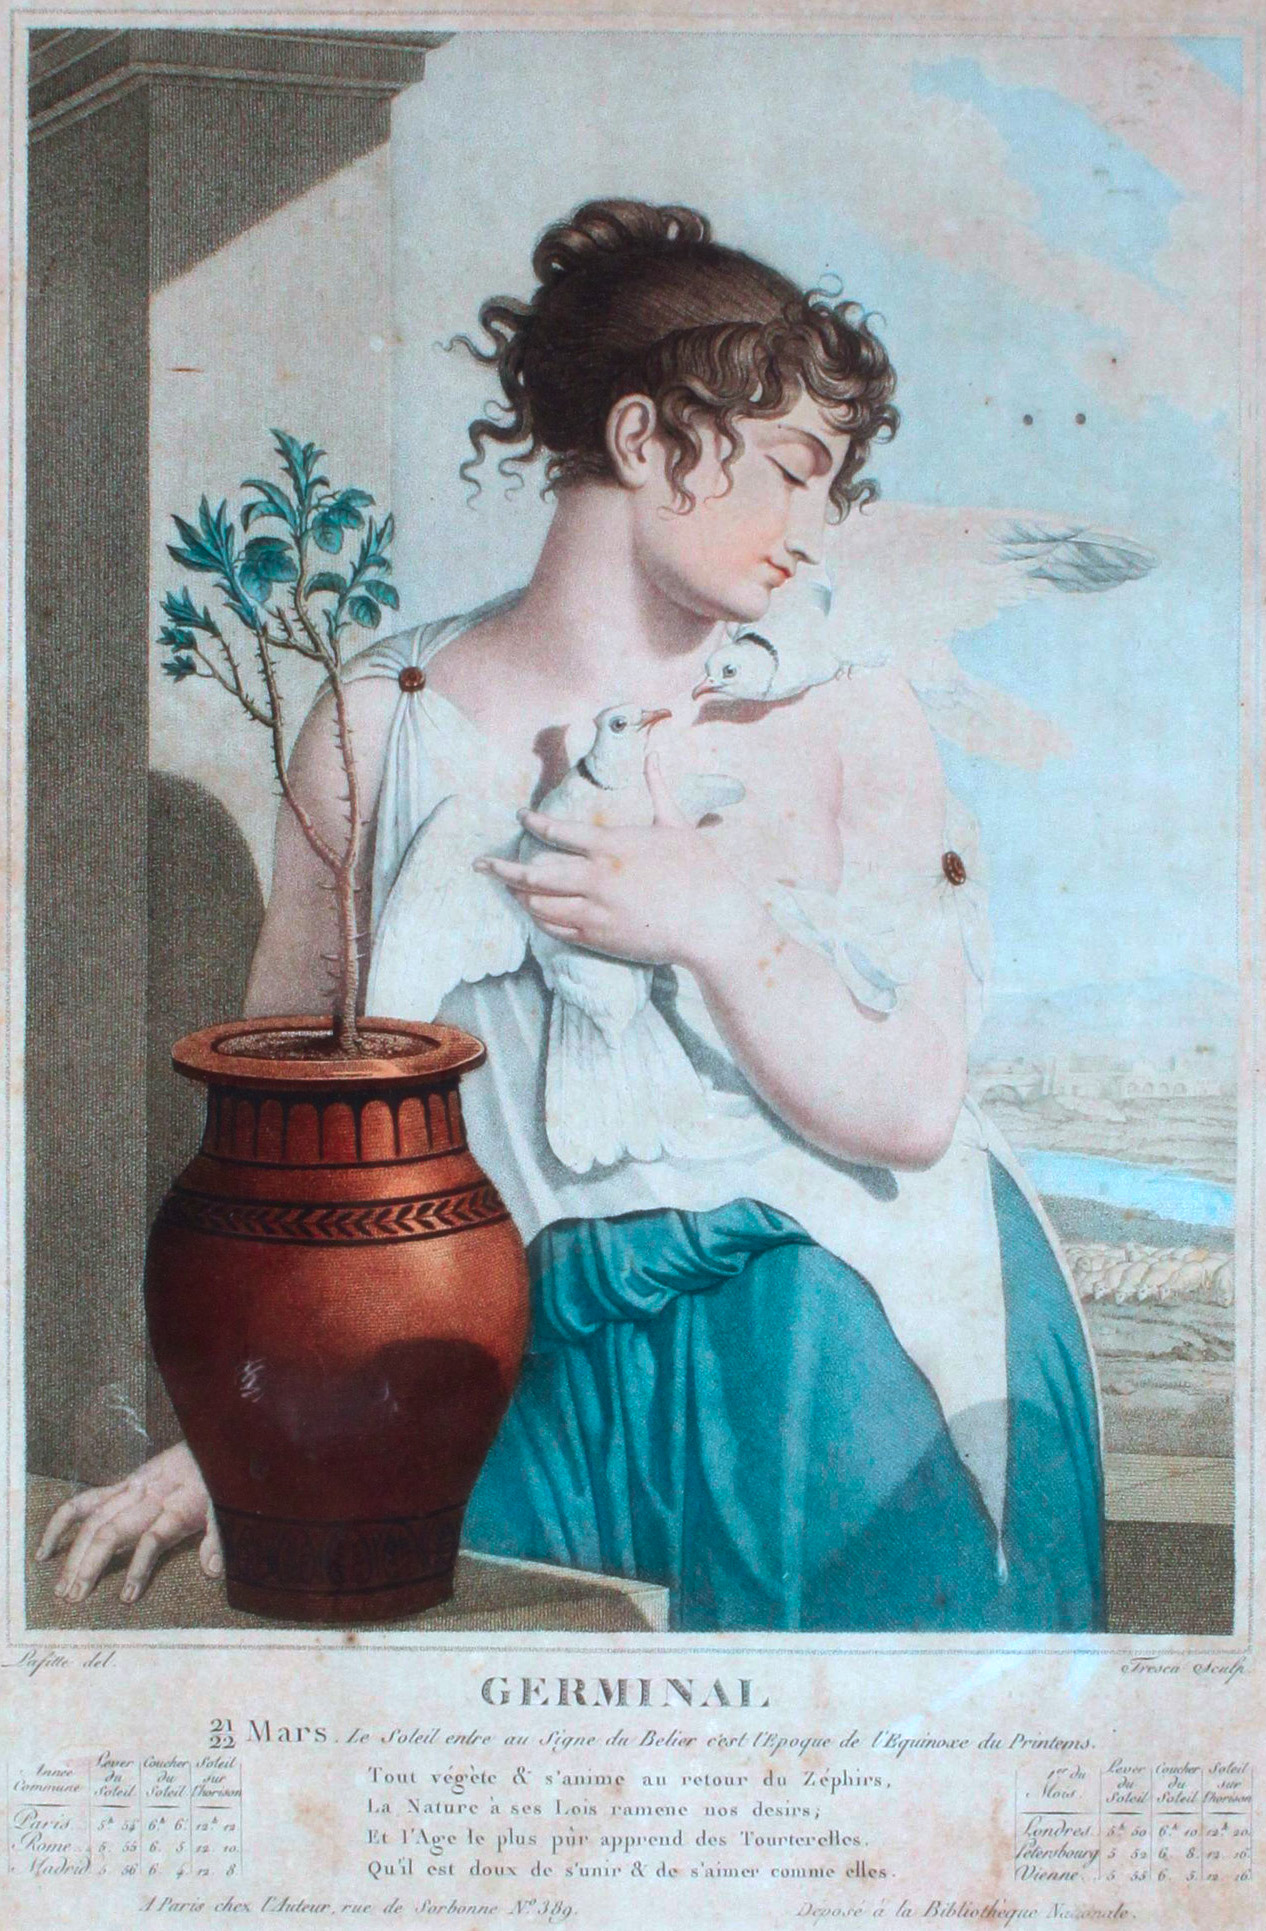
\includegraphics[width=\linewidth]{fig/germinal.jpg}
    \caption{\emph{Allégorie pour le mois de Germinal}, Louis Lafitte.}
\end{marginfigure}

A configuration of a "Turing machine"---or more generally the node of an
"automatic graph"---is said 
to be \AP""germinal"" if it has in-degree 0.%
\sidenote{A natural terminology would be ``initial'' but it clashes with the well-established notion of "initial configuration".}

\kregcolundec%

\begin{proof}%
	\proofcase{Lower bound.}
    By reduction from the "reachable regularity problem" for "linear Turing machines"
    (\Cref{lem:reachable-regularity}). We first show it for $k=2$.

    \AP Given a "linear Turing machine" $\+T$,
    observe that the set $\intro*\Germ{\+T}$ of all "germinal configurations" of $\confGraph$.
    \begin{claim}
        $\Germ{\+T}$ is effectively a "regular language". 
    \end{claim}
    
    Observe moreover that, by definition of "linear Turing machines",
    the "initial configuration" $\pad\cdot q_0 \cdot \pad$ is "germinal".
    Let $\bSymb$ and $\rSymb$ be fresh symbols. 
    Consider the "automatic graph" $\tup{V,\+E}$ for $V \defeq \configs\cdot (\bSymb + \rSymb)$,
    having an edge from $\gamma \cdot c$ to $\gamma' \cdot c$ if either 
    \begin{enumerate}
        \item $\tup{c,c'} = \tup{\bSymb,\rSymb}$ and $\gamma=\gamma'$;
        \item $\tup{c,c'} = \tup{\rSymb,\bSymb}$ and there is an edge from $\gamma$ to $\gamma'$ in $\confGraph$; or
        \item $\tup{c,c'} = \tup{\bSymb,\bSymb}$, $\gamma$ is the "initial configuration",
        and $\gamma' \neq \gamma$ is "germinal".
    \end{enumerate}

    \begin{marginfigure}%
        \centering
        \begin{tikzpicture}
            \input{tikz/dichotomy/conf-graph-wf-RTM}
        \end{tikzpicture}
        \caption{
            \AP\label{fig:reduction-wf-RTM-to-colouring-config-graph-wf-RTM}
            Configuration graph of a "linear Turing machine".
        }
    \end{marginfigure}%
    \begin{marginfigure}%
        \centering
        \begin{tikzpicture}
            \input{tikz/dichotomy/reduction-wf-RTM}
        \end{tikzpicture}
        \caption{
            \AP\label{fig:reduction-wf-RTM-to-colouring}
            The "automatic graph" to which the "configuration graph"
            of \Cref{fig:reduction-wf-RTM-to-colouring-config-graph-wf-RTM} is reduced.
        }
    \end{marginfigure}%

    Symbols $\bSymb$ and $\rSymb$ are utilized to represent two versions of each configuration.
    This graph is depicted in \Cref{fig:reduction-wf-RTM-to-colouring}.
    Note that $\tup{V,\+E}$ is "connected" and "2-colourable": in fact, it is a "directed tree" whose root is $\pad\cdot q_0\cdot \pad\cdot \bSymb$. 
    
    We claim that $\tup{V,\+E}$ is "regularly $2$-colourable" if, and only if, the set of "reachable configurations" of $T$ is a "regular language". 
    In fact, up to permuting the two-colours, $\tup{V,\+E}$
    admits a unique 2-colouring $\tup{C_1,C_2}$, defined by:
    \[
        C_1 \defeq \Reach{\+T}\cdot\bSymb \cup (\configs \setminus \Reach{\+T})\cdot\rSymb
    \]
    and $C_2$ is the complement of $C_1$.
    If $\Reach{\+T}$ is regular, then so is $C_1$. Dually, if $C_1$ is regular, then
    $\Reach{\+T}$ is exactly the set of configurations $\gamma$ such that
    $\gamma\cdot \bSymb \in C_1$ and hence is regular.
    It follows that $\tup{V,\+E}$ is "regularly $2$-colourable" if and only if
    the "reachable configurations" of $\+T$ are regular, which concludes the proof for $k=2$.

    To prove the statement for any $k>2$, we define $\tup{V,\+E_k}$ as the result of adding a $(k-2)$-clique to $\tup{V,\+E}$ and adding an edge from every vertex of the clique to every vertex incident to an edge of $\+E$. This forces the clique to use $k-2$ colours that cannot be used in the remaining part of the graph and the proof is then analogous.

	\proofcase{Upper-bound.} We show that the problem is "RE". Let us define a \AP""$k$-coloured automaton"" like a regular (complete) DFA, except that instead of having
	a set of final states, it has a partition $\langle C_1,\hdots,C_k \rangle$ of its states.
	Such an automaton recognizes a "regular colouring" $\Sigma^* \to \lBrack 1, k\rBrack$.
	Given an "automatic graph" $\+G = \tup{V,\+E}$---whose edge relations is given by
    a "synchronous automaton" $\relPres{\+E}{\+G}$---and a $k$-coloured automaton $\+B$,
	we can build, by a product construction, an automaton $\+A'$ which accepts
	all $u \otimes v \in \convolRel{R}$ such that the colour of $u$ is distinct from
    the colour of $v$.
	Then, $\+A'$ is equivalent to $\relPres{\+E}{\+G}$ if, and only if,
    $\+B$ describes a proper "$k$-colouring" of $\tup{V,\+E}$.
    The "RE" upper-bound of the "regular $k$-colourability problem" follows: 
    it suffices to enumerate all "$k$-coloured automata" and check for equivalence.
\end{proof}

Note that this reduction provides an easy way of building
graphs in the shape of \Cref{fig:reduction-wf-RTM-to-colouring} that are "2-colourable" (in fact, they are trees) but not "regularly $2$-colourable". In fact, we can provide a slightly more
direct construction.

\begin{figure}
    \centering
    \begin{tikzpicture}
        \input{tikz/dichotomy/tree-not-2reg-colour}
    \end{tikzpicture}
    \caption{
        \label{fig:tree-not-2reg-colour}
        The "automatic tree@automatic graph" $\+T$ of \Cref{ex:tree-not-2-reg-colourable},
        and its unique "$2$-colouring" $(C, V\setminus C)$, which is not "regular@@colouring".
    }
\end{figure}
\begin{example}
    \AP\label{ex:tree-not-2-reg-colourable}
    On the alphabet $\Sigma = \{a,b\}$, the tree $\+T$ depicted in \Cref{fig:tree-not-2reg-colour} whose set of vertices is $V = a^*b^*$ and whose set 
    of edges is $\+E = \+E_{\mathrm{incr}} \cup \+E_{\mathrm{init}}$, with 
    \begin{align*}
        \+E_{\mathrm{incr}} & = \{(a^pb^q,\, a^{p+1}b^{q+1}) \mid p,q \in \N\} \\
        \+E_{\mathrm{init}} & = \{(\varepsilon,\, a^p) \mid p \in \N\} \cup \{(\varepsilon,\, b^q) \mid q \in \N\}, 
    \end{align*}    
    is "automatic@automatic graph" but not "regularly $2$-colourable".
    Indeed, its only "$2$-colouring"
    consists in partitioning the vertices of $\+T$ into
    \begin{align*}
        C =\;& \{a^n b^n \mid n \in 2\N\} \\
            & \cup \{a^p b^q \mid p > q \text{ and $q$ is odd}\} \\
            & \cup \{a^p b^q \mid p < q \text{ and $p$ is odd}\}
    \end{align*}
    and its complement $V \setminus C$.
    Let $P = \{a^p b^q \mid p, q \in 2\N\} = (aa)^*(bb)^*$:
    $P$ is regular, yet $C \cap P = \{a^n b^n \mid n \in 2\N\}$ is not.
    Hence, $C$ is not regular, and thus $\+T$ is not "regularly $2$-colourable".
\end{example}
\subsection{Bounded Recognizable Relations}

\paragraph*{Separability for Bounded Recognizable Relations.}

In this section we capitalize on the undecidability result of the previous section, showing how this implies the undecidability for the "separability problem" on two natural classes of bounded "recognizable relations", namely: $\kREC$, and $\kPROD$.
Remember that, for any $k$, $\reintro*\kPROD$ is the subclass of $\REC$ consisting of unions of $k$ cross-products of regular languages (which is a subclass of $\kREC[2^{2k}]$).

First, observe that the $\kREC[1]$-"separability problem" is trivially decidable, since the only possible "separator" is $\Sigma^* \times \Sigma^*$. However, for any other $k>1$, the problem is undecidable.

\begin{proposition}
    The $\kREC$-"separability problem" is undecidable, for every $k>1$.
\end{proposition}
\begin{proof}
A consequence of the reduction from the "$k$-regular colourability problem" of \Cref{thm:reg-colourability-equiv-separability}, combined with the undecidability of the latter for every $k>1$ (\Cref{thm:k-reg-col-undec}).
\end{proof}

On the $\kPROD$ hierarchy we will find the same phenomenon. In particular the case $k=1$ is also trivially decidable.

\begin{proposition}
    The $\kPROD[1]$-"separability problem" is decidable.
\end{proposition}
\begin{proof}
    Given two "automatic relations" $R_1, R_2$, there exists $S \in $ \kPROD[1]
    that "separates" $R_1$ from $R_2$ if and only if $\pi_1(R_1)\times \pi_2(R_1)$
    "separates" $R_1$ from $R_2$.
\end{proof}

As soon as $k>1$, the $\kPROD$ "separability problem" becomes undecidable. This is a consequence of the following simple lemma.

\begin{lemma}
    A symmetric "automatic relation" $R$ and the identity $\Id$ are "separable" by a relation in $\kPROD[2]$ iff they have a "separator" of the form $(A \times B) \cup (B \times A)$.
\end{lemma}
\begin{proof}
    Assume that $S \in \kPROD[2]$ "separates" $R$ from $\Id$.
    Then $R \subseteq S$, but since $R$ is symmetric, $R = R^{-1} \subseteq S^{-1}$ so
    $R \subseteq S \cap S^{-1}$, and hence $R \subseteq S \cap S^{-1}$.
    Moreover, since $S$ has a trivial intersection with $\Id$, so does $S \cap S^{-1}$.
    Hence, $S \cap S^{-1}$ "separates" $R$ from $\Id$.

    Since $S \in \kPROD[2]$, there exists $A_1,A_2,B_1,B_2 \subseteq \Sigma^*$ such that
    $S = A_1 \times B_1 \cup B_2 \times A_2$.
    Note that $S \cap \Id = \emptyset$ yields $A_i \cap B_i = \emptyset$ for each $i \in \{1,2\}$.
    Finally:
    \begin{align*}
        S \cap S^{-1} &
        =
            \bigl( A_1 \times B_1 \cup B_2 \times A_2 \bigr)
            \cap \bigl( B_1 \times A_1 \cup A_2 \times B_2 \bigr) \\
        &
        =
            \bigl( (A_1 \times B_1) \cap (B_1 \times A_1) \bigr)
            \cup \bigl( (A_1 \times B_1) \cap (A_2 \times B_2) \bigr) \\
        &
        \hphantom{=\;} \cup \bigl( (B_2 \times A_2) \cap (B_1 \times A_1) \bigr)
            \cup \bigl( (B_2 \times A_2) \cap (A_2 \times B_2) \bigr) \\
        &
        =
            \bigl( \overbrace{(A_1 \cap B_1) \times (A_1 \cap B_1)}^{= \emptyset} \bigr)
            \cup \bigl( (A_1 \cap A_2) \times (B_1 \cap B_2) \bigr) \\
        &
        \hphantom{=\;} \cup \bigl( (B_1 \cap B_2) \times (A_1 \cap A_2) \bigr)
            \cup \bigl( \underbrace{(A_2 \cap B_2) \times (A_2 \cap B_2)}_{= \emptyset} \bigr)\\
        &
        = \bigl( (A_1 \cap A_2) \times (B_1 \cap B_2) \bigr)
            \cup \bigl( (B_1 \cap B_2) \times (A_1 \cap A_2) \bigr).\qedhere
    \end{align*}
\end{proof}

We can then establish the following: 

\begin{corollary}\AP\label{cor:2reg-2prod}
    A symmetric "automatic relation" $R$ and $\Id$ are "separable" by a relation in $\kPROD[2]$ if{f} $\AutGraph{\Sigma^*}{R}$ is "$2$-regular colourable".
\end{corollary}
\begin{proof}
    By observing that for any symmetric relation $R \subseteq \Sigma^* \times \Sigma^*$, we have that $A,B \subseteq \Sigma^*$ is a colouring of $\AutGraph{\Sigma^*}{R}$ if, and only if, $(A \times B) \cup (B \times A)$ "separates" $R$ from $\Id$.
\end{proof}

We can now easily show undecidability for the $\kPROD[2]$ "separability problem" by reduction from the "$2$-regular colourability problem".
\begin{lemma}\AP\label{lem:aut-2prod-sep-undec}
    The $\kPROD[2]$-"separability problem" is undecidable.
\end{lemma}
\begin{proof}
    By reduction from the "$2$-regular colourability problem" on "automatic graphs", which is undecidable by \Cref{thm:k-reg-col-undec}. Let $\AutGraph{L}{R}$ be an "automatic graph" and $\AutGraph{L}{R'}$ the symmetric closure of $\AutGraph{L}{R}$. It follows that $\AutGraph{L}{R'}$ is still "automatic" and that there is a "$2$-regular colouring" for $\AutGraph{L}{R'}$ if{f} there is a "$2$-regular colouring" for $\AutGraph{L}{R}$ (the same colouring in fact).
    Thus, by \Cref{cor:2reg-2prod}, $\AutGraph{L}{R}$ is "$2$-regular colourable" if{f} 
    there is a $\kPROD[2]$ relation that "separates" $R'$ from $\Id$.
\end{proof}

Further, this implies undecidability for every larger $k$:
\begin{theorem}
    \AP\label{thm:kprod-undecidable}
    The $\kPROD$-"separability problem" is undecidable, for every $k \geq 2$.
\end{theorem}

\begin{figure}
    \centering
    \begin{tikzpicture}
        \input{tikz/dichotomy/2prod-to-kprod}
    \end{tikzpicture}
    \caption{
        \AP\label{fig:2prod-to-kprod}
        Construction in the proof of \Cref{thm:kprod-undecidable} for $k = 5$. $S$ is depicted as the union of two (gray) rectangles since $S \in \kPROD[2]$.
        The relation $R'_1$ is obtained from $R_1$ (blue shape) by adding all blue edges,
        namely $(a_i, b_i)$ for $1\leq i \leq k-2$. The relation $R'_2$ is obtained from $R_2$ (red shape) by adding
        all red edges, namely every other edge involving a vertex $a_i$ or $b_i$.
        Finally, $S'$ (five gray rectangles) is obtained from $S$ by adding
        each $\{a_i\} \times \{b_i\}$.
    }
\end{figure}

\begin{proof}
    The case $k=2$ is shown in \Cref{lem:aut-2prod-sep-undec}, so suppose $k>2$.
    The proof goes by reduction from the $\kPROD[2]$-"separability problem". Let $R_1,R_2$ be a pair of "automatic relations" over an alphabet $\Sigma$. Consider the alphabet extended with $2(k-2)$ fresh symbols $\Sigma' = \Sigma \dcup \set{a_1, \dotsc, a_{k-2}, b_1, \dotsc, b_{k-2}}$. We build "automatic relations" $R'_1,R'_2$ over $\Sigma'$ such that $(R_1,R_2)$ are $\kPROD[2]$ "separable" over $\Sigma$ if{f} $(R'_1,R'_2)$ are $\kPROD$ "separable" over $\Sigma'$.

    Let $R'_1 = R_1 \dcup \set{ (a_i,b_i) : 1 \leq i \leq k-2}$ and 
    \begin{align*}
    R'_2 =  R_2 \dcup {}&\set{(a_i,w) : w \in \Sigma^*, 1 \leq i \leq k-2} \dcup {}\\
                    &\set{(w,b_i) : w \in \Sigma^*, 1 \leq i \leq k-2} \dcup {}\\
                    &\set{(a_i,b_j) : 1 \leq i,j \leq k-2, i \neq j} \dcup {}\\
                    &\set{(b_i,a_j) : 1 \leq i,j \leq k-2}
    \end{align*}
    
    If $(R_1,R_2)$ has a $\kPROD[2]$ "separator" $S$, then $\tilde S \dcup \set{(a_i,b_i) : 1 \leq i \leq k-2}$ is a $\kPROD$ "separator" of $(R'_1,R'_2)$.
    

    Conversely, if $S' = (A_1 \times B_1) \cup \dotsb \cup (A_k \times B_k)$ is a $\kPROD$ "separator" of $(R'_1,R'_2)$, then for every $i$ there must be some $j_i$ such that $A_{j_i} \times B_{j_i}$ contains $(a_i,b_i)$. Observe that 
    \begin{itemize}
        \item $A_{j_i} \cup B_{j_i}$ cannot contain any $a_{i'}$ or $b_{i'}$ for $i' \neq i$, and
        \item $A_{j_i} \cup B_{j_i}$ cannot contain any $w \in \Sigma^*$;
    \end{itemize}
    since otherwise we would have $(A_{j_i} \times B_{j_i}) \cap R'_2 \neq \emptyset$.
    Hence, $\set{i \mapsto j_i}_i$ is injective, and thus $S'$ is of the form $S' = (A_1 \times B_1) \cup (A_2 \times B_2)  \cup (\set{a_1} \times \set{b_1}) \cup \dotsb \cup (\set{a_{k-2}} \times \set{b_{k-2}})$. We can further assume that $A_1,B_1,A_2,B_2$ do not contain any $a_i$ or $b_i$ since otherwise we can remove them preserving the property of being a $\kPROD$ "separator" of $R'_1$ and $R'_2$.
    Hence, $S \defeq (A_1 \times B_1) \cup (A_2 \times B_2)$ must cover $R_1$ and be disjoint from $R_2$, obtaining that $S$ is a $\kPROD[2]$ "separator" of $R_1$ and $R_2$.
\end{proof}


\paragraph*{Definability for Bounded Recognizable Relations.}
Up until now, we have examined two hierarchies of bounded recognizable relations, namely $\kPROD$ and $\kREC$. 
Our previous analysis demonstrated that, for any element in these hierarchies (where $k>1$), the "separability problem" is undecidable. Nevertheless, 
we will now establish that the "definability problem" is decidable.

\AP Given an "automatic" relation $R \subseteq \Sigma^* \times \Sigma^*$, consider the "automatic" equivalence relation $\intro*\autequiv \subseteq \Sigma^* \times \Sigma^*$, defined as $w \mathrel{\autequiv} w'$ if for every $v \in \Sigma^*$ we have 
\begin{enumerate}
    \item $(w,v) \in R$ if{f} $(w',v) \in R$, and
    \item $(v,w) \in R$ if{f} $(v,w') \in R$.
\end{enumerate}

It turns out that equivalence classes of $\autequiv$ define the coarsest partition onto which $R$ can be recognized in terms of $\kREC$:

\begin{lemma}\AP\label{lem:krec-characterization}
    For every "automatic" $R \subseteq \Sigma^* \times \Sigma^*$, $\autequiv$ has index at most $k$ if, and only if, $R$ is in $\kREC$.
\end{lemma}
\begin{proof}
    \proofcase{Left-to-right}
    Assume that $\autequiv$ has the equivalence classes $E_1, \dotsc, E_k$. Consider the set $P \subseteq \set{1, \dotsc, k}^2$ of all pairs $(i,j)$ such that there are $u_i \in E_i$ and $u_j \in E_j$ with $(u_i,u_j) \in R$. Define the $\kREC$ relation $R' = \bigcup_{(i,j) \in P} E_i \times E_j$. We claim that $R=R'$. 
    In fact, by definition of $\autequiv$, note that if there are $u_i \in E_i$ and $u_j \in E_j$ with $(u_i,u_j) \in R$, then $E_i \times E_j \subseteq R$. Hence, $R' \subseteq R$.
    On the other hand, for every pair $(u,v) \in R$ there is $(i,j) \in P$ such that $u \in E_i$, $v \in E_j$ implying $(u,v) \in R'$.
    Hence, $R \subseteq R'$.

    \proofcase{Right-to-left}
    If $R$ is a union of products of sets from the partition $E_1 \dcup \dotsb \dcup E_k = \Sigma^*$, then every two elements of each $E_i$ are $\autequiv$-related, and thus $\autequiv$ has index at most $k$.
\end{proof}

We can then conclude that the definability problem for $\kREC$ is decidable. 

\begin{corollary}
    The $\kREC$-"definability problem" is decidable, for every $k > 0$.
\end{corollary}
\begin{proof}
    An "automatic relation" $R$ is in $\kREC$ if{f} $\autequiv$ has at most $k$ equivalence classes by \Cref{lem:krec-characterization}. 
    % This can be tested with the formula $\forall w_1, \dotsc, w_{k+1} ~ \bigvee_{i \neq j} w_i \mathrel{\autequiv} w_j$.
    %    
    In other words, an "automatic relation" $R$ is not in $\kREC$ if{f} the complement of $\autequiv$ contains a $(k+1)$-clique, which can be easily tested.
\end{proof}

The relation $\autequiv$ can also be used to characterize which automatic relations are definable in the class $\kPROD$.

\begin{lemma}
    An "automatic relation" $R$ is in $\kPROD$ if, and only if, $R=(A_1 \times B_1) \cup \dotsb \cup (A_k \times B_k)$ where each $A_i$ and $B_i$ is a union of equivalence classes of $\autequiv$.
\end{lemma}
\begin{proof}
    It suffices to show that for every equivalence class $E$ from $\autequiv$, if $A_1 \cap E \neq \emptyset$ then $R = ((A_1 \cup E) \times B_1) \cup \dotsb \cup (A_k \times B_k)$, and similarly for $B_1$. Assume $w \in A_1 \cap E$ and take any pair $(u,v) \in E \times B_1$. We show that $(u,v) \in R$. By definition of $\autequiv$, since $(w,v) \in R$ and $w \mathrel{\autequiv} u$, we have that $(u,v) \in R$.
\end{proof}

Again, this characterization allows us to show that definability in the class $\kPROD$ is decidable. 

\begin{corollary}
    The $\kPROD$-"definability problem" is decidable, for every $k > 0$.
\end{corollary}

\begin{proof}
    By brute force testing whether the "automatic relation" $R$ is equivalent to $(A_1 \times B_1) \cup \dotsb \cup (A_k \times B_k)$ for every possible $A_i,B_i$ which is a union of equivalence classes of $\autequiv$.
\end{proof}

\section{Undecidability of the Homomorphism Problems}
\label{sec:dichotomy-undecidability}

\subsection{Overview \& Easy Implications of the Dichotomy Theorem}
\label{sec:dichotomy-overview}

\begin{mainstatement}
	\DichotomyThmDichotomyAutomatic
\end{mainstatement}

\begin{remark}
	\todo{TODO GEneralization to "higher-order automatic structures".}
	\todo{Deterministic rational?}
	\todo{RHS is "automatic@@struct"?}
\end{remark}

\begin{marginfigure}
	\centering
	\begin{tikzpicture}
		\node (1) at (0,0) {\itemDTFinDual};
\node[below=2em of 1] (5) {\itemDTFirstOrder};
\node[below=2em of 5] (4) {\itemDTEqual};
\node[below left=2em and -1em of 4] (3) {\itemDTHomRegDec};
\node[below right=2em and -1em of 4] (2) {\itemDTHomDec};

% ---
% Transitions
% ---
\draw[implication] (1) to (5);
\draw[implication] (5) to (4);
\draw[implication] (4) to (3);
\draw[implication] (4) to (2);
\draw[implication, bend left=30] (3) to (1.west);
\draw[implication, bend right=30] (2) to (1.east);
	\end{tikzpicture}
	\caption{\AP\label{fig:dichotomy-overview}Implications shown in the chapter to prove
	\Cref{thm:dichotomy-theorem-automatic-structures}.}
\end{marginfigure}
We prove \Cref{thm:dichotomy-theorem-automatic-structures} by showing the
implications depicted in \Cref{fig:dichotomy-overview}.
The most difficult implications are $\itemDTFinDual \Rightarrow \itemDTFirstOrder$,
which we prove in \Cref{sec:dichotomy-decidability}, and the implications
$\itemDTHomDec \Rightarrow \itemDTFinDual$ and $\itemDTHomRegDec \Rightarrow \itemDTFinDual$,
which we prove by contraposition in \Cref{sec:undecidability-hom,sec:undecidability-homreg}.

On the other hand, the implications $\itemDTFirstOrder \Rightarrow \itemDTEqual$,
$\itemDTEqual \Rightarrow \itemDTHomRegDec$ and $\itemDTEqual \Rightarrow \itemDTHomDec$ are straightforward: we prove them in this section. 
Before showing these implications, we start by proving $\itemDTFinDual \Rightarrow \itemDTHomDec$.\footnote{While it is redundant with the implications of \Cref{fig:dichotomy-overview}, 
we prove this implication for two reasons: not only is it straightforward, it is also
the implication which, together with the fact that both $\HomAut{\clique{2}}$
and $\HomRegAut{\clique{2}}$ are undecidable by
\cite[Proposition 6.5]{Kocher2014AutomatischenGraphen}
and \cite[Theorem 4.4]{BarceloFigueiraMorvan2023SeparatingAutomatic}, that lead us to conjecture
\Cref{thm:dichotomy-theorem-automatic-structures}.}

\paragraph*{Decidability of the Homomorphism Problem.}

\begin{proposition}
	\!\footnote{This corresponds to the implication $\itemDTFinDual \Rightarrow \itemDTHomDec$
	of \Cref{thm:dichotomy-theorem-automatic-structures}.}
	\AP\label{prop:dichotomy-FinDual-implies-HomDec}
	Let $\?B$ be a "finite $\sigma$-structure".
	If $\?B$ has finite duality, then $\HomAut{\?B}$ is decidable in "NL".
\end{proposition}

\begin{proof}
	Given a "finite $\sigma$-structure" $\?D$ with domain $\{d_1,\hdots,d_n\}$,
	we build the "first-order sentence"
	\[
		\phi_{\?D} \defeq \exists x_1.\; \cdots \exists x_n.\;
		\bigwedge_{\+R_{(k)} \in \sigma} \bigwedge_{\substack{\tup{i_1,\hdots,i_k} \in \lBrack 1,n\rBrack^k\\\text{"st" }\tup{d_{i_1},\hdots,d_{i_k}} \in \+R(\?D)}}
		\+R(x_{i_1},\hdots,x_{i_k}).
	\]
	By construction, for any arbitrary "$\sigma$-structure" $\?A$, we have $\?A \FOmodels \phi_{\?D}$
	"iff" $\?D \homto \?A$.
	Then, since $\?B$ has "finite duality", it admits a finite "dual"
	$\?D_1,\hdots,\?D_m$.
	Then
	\[
		\?A \FOmodels \bigwedge_{i=1}^m \neg \phi_{\?D_i}
		\quad\text{"iff"}\quad 
		\?A \homto \?B.
	\]
	The conclusion follows from the fact that the "data complexity"
	of "first-order model checking of automatic structures" is "NL"
	by \Cref{prop:first-order-model-checking-automatic-structures}.
\end{proof}

Note that \Cref{prop:dichotomy-FinDual-implies-HomDec} still holds
when the "homomorphism problem" takes as input "higher-order automatic
structures" since such structures have a decidable first-order theory.


\paragraph*{Uniformly First-Order Definable Homomorphisms Imply Equality.}

\begin{proposition}
	\!\footnote{This corresponds to the implication $\itemDTFirstOrder \Rightarrow \itemDTEqual$
	of \Cref{thm:dichotomy-theorem-automatic-structures}.}
	\AP\label{prop:dichotomy-FirstOrder-implies-Equal}.
	Let $\?B$ be a "finite $\sigma$-structure".
	If $\HomAll{\?B}$ has "uniformly first-order definable homomorphisms", then
	$\HomAut{\?B} = \HomRegAut{\?B}$.
\end{proposition}

\begin{proof}
	By assumption,there exists "first-order formulas"
	$\langle \phi_b(x) \rangle_{b\in B}$ over $\sigma$ "st" for any
	arbitrary "$\sigma$-structure" $\?A$, for any $a\in A$,
	there is at most one $b \in B$ "st" $\langle \?A, a \rangle \FOmodels \phi_b(x)$, and moreover $\?A \homto \?B$
	"iff" for each $a\in A$, there is exactly one $b(a) \in B$ "st" $\langle \?A, a \rangle \FOmodels \phi_{b(a)}(x)$, and $a \mapsto b(a)$ is a "homomorphism".
	Now, when the right-hand side holds, given an "automatic structure" $\+A$,
	for each $b\in \?B$, we let $\tilde\phi_b(x)$ be the "first-order formula" over $\signatureSynchronous{\Sigma}$ obtained from $\phi_b(x)$
	by substituting $\+R(x_1,\hdots,x_k)$ for the "first-order formula"
	over $\signatureSynchronous{\Sigma}$ describing $\+R_{(k)}$ in $\+A$.
	It follows that if $\?A \homto \?B$, then the function
	mapping $u \in \Sigma^*$ to the unique $b \in B$ "st" $\Sigma^*, u \FOmodels \tilde\phi_b(x)$
	defines a "regular homomorphism" from $\+A$ to $\?B$---the regularity follows from
	todo:addref-first-order-iff-automatic.
	And hence $\HomAut{\?B} \subseteq \HomRegAut{\?B}$. The conclusion follows since
	the other implication is trivial.
\end{proof}

\paragraph*{Equality of the Homomorphism Problems Imply their Decidability.}

\begin{proposition}
	\!\footnote{This corresponds to the implication $\itemDTEqual \Rightarrow \itemDTHomDec$
	of \Cref{thm:dichotomy-theorem-automatic-structures}.}
	\AP\label{prop:dichotomy-Equal-implies-HomDec}.
	Let $\?B$ be a "finite $\sigma$-structure".
	If $\HomAut{\?B} = \HomRegAut{\?B}$ then $\HomAut{\?B}$ and $\HomRegAut{\?B}$
	are decidable.
\end{proposition}

To prove this, we first give an upper bound on the homomorphism problems independently
of any assumption on $\?B$.
\begin{proposition}
	\AP\label{prop:dichotomy-general-upper-bounds}
	Let $\?B$ be a "finite $\sigma$-structure".
	Then $\HomAut{\?B}$ is "coRE" and $\HomRegAut{\?B}$ is "RE".
\end{proposition}

\begin{proof}
	\proofcase{$\HomAut{\?B}$ is "coRE".}
	By the "De Bruijn–Erdős Theorem", for any arbitrary "$\sigma$-structure" $\?A$,
	we have $\?A \nothomto \?B$ "iff" there exists a finite "substructure" $\?A'$ of $\?A$
	"st" $\?A' \nothomto \?B$.
	Given a "finite $\sigma$-structure" $\?A'$ and an "automatic $\sigma$-structure",
	it is decidable whether $\?A'$ is a "substructure" of $\?A$: indeed, it suffices
	to check, using \Cref{prop:first-order-model-checking-automatic-structures} if
	\[
		\Bigl(
			\exists x_1,\; \cdots \exists x_n,\;
			\bigwedge_{\+R_{(k)} \in \sigma} \bigwedge_{\substack{\tup{i_1,\hdots,i_k} \in \lBrack 1,n\rBrack^k\\\text{"st" }\tup{a_{i_1},\hdots,a_{i_k}} \in \+R(\?A')}}
			\+R(x_{i_1},\hdots,x_{i_k})
		\Bigr)
		\FOmodels^{?} \?A,
	\]
	by letting $\{a_1,\hdots,a_n\} = A'$. 
	Moreover, whether $\?A' \nothomto \?B$ is also decidable---in "coNP"---by \todo{addref}.
	Overall, this provides a co-semi-algorithm for $\HomAut{\?B}$: we enumerate finite
	"$\sigma$-structure" $\?A'$, and test if (1) $\?A'$ is a "substructure" of $\?A$ and if (2)
	$\?A' \homto \?B$. And hence $\HomAut{\?B}$ is "coRE".

	\proofcase{$\HomRegAut{\?B}$ is "RE".} This is an easy generalization of
	\Cref{thm:k-reg-col-undec}: instead of having "$k$-coloured automaton", we define
	``$\?B$-automaton'', that admit a partition $\langle C_{b} \rangle_{b \in B}$.
	The semantics of such an automaton is a partial function $f\colon \Sigma^* \to B$. 
	Given an "automatic structure" $\+A$, we can then effectively test if $f$ is defined on $\domainPres{\+A}$, and if $f$ defines a "homomorphism" from $\?A$ to $\?B$---see
	the proof of \Cref{thm:k-reg-col-undec}. If so, $\+A \homregto \?B$. Dually, any "regular homomorphism" $\+A \homregto \?B$ can be described by such a $\?B$-automaton.
	Therefore, $\HomRegAut{\?B}$ is "RE".
\end{proof}

\begin{proof}[Proof of \Cref{prop:dichotomy-Equal-implies-HomDec}.]
	If $\HomAut{\?B} = \HomRegAut{\?B}$, then by \Cref{prop:dichotomy-general-upper-bounds},
	these problems are both "RE" and "coRE", and are hence decidable.
\end{proof}

\subsection{Undecidability of \,$\HomAut{\?B}$}
\label{sec:undecidability-hom}

We now prove the undecidability of $\HomAut{\?B}$ and $\HomRegAut{\?B}$
when $\?B$ does not have "finite duality". Both reductions are
direct adaptations of the proof that $\HomFin{\?B}$ is "L"-hard when $\?B$ does not
have finite duality by \textcite[Theorem 3.2]{LaroseTesson2009UniversalAlgebraCSP}.
However, proving the undecidability of the problem that is reduced
to $\HomRegAut{\?B}$ is not entirely trivial and requires some work.
\begin{itemize}
	\item For $\HomFin{\?B}$, we reduce the complement of "Connectivity in automatic graphs",
		providing a "coRE"-lowerbound.
	\item For $\HomRegAut{\?B}$, we reduce "regular unconnectivity in automatic graphs",
		which in turn is reduced from \todo{update}.
\end{itemize}

For $n\in\N$, we define the \AP""$n$-link"" $\intro*\link{n}$ be the "$\sigma$-structure"\sidenote{From \cite[\S~2]{LaroseLotenTardif2007CharacterisationFOCSP}.} 
whose domain is $\lBrack 0,n\rBrack$, and every "predicate" $\+R$
of arity $k$, is interpreted as the set of tuples $\langle a_1,\, \hdots,\, a_k \rangle$
"st" $|a_i-a_j| \leq 1$ for all $i,j \in \lBrack 0,n \rBrack$. See \Cref{fig:n-link}.
\begin{marginfigure}
	\centering
	\begin{tikzpicture}
		\node[vertex] (0) at (0,0) {};
\node[vertex, right=of 0] (1) {};
\node[vertex, right=of 1] (2) {};
\node[vertex, right=of 2, opacity=0] (3) {};
\node[vertex, right=of 3] (4) {};
\node[yshift=-.1em] at (3) (3-label)  {$\cdots$};

% ---
% Transitions
% ---
\foreach \i in {0,1,2,3} {
	\pgfmathtruncatemacro{\next}{\i + 1}
	\draw[edge, bend right=30] (\i) to (\next);
	\draw[edge, bend right=30] (\next) to (\i);
};
\foreach \i in {0,1,2,4} {
	\draw[edge, loop, out=60,in=120,looseness=6] (\i) to (\i);
}
	\end{tikzpicture}
	\caption{\AP\label{fig:n-link}The "$n$-link" $\link{n}$ over the "graph signature".}
\end{marginfigure}
Given a "$\sigma$-structure" $\?B$, say that $b \in \?B$ and $b'$ are
\AP""$n$-linked"" if there exists a "homomorphism" from $\link{n}$ to $\?B$
that sends $0$ to $b$ and $n$ to $b'$. We say that $b$ and $b'$ are \AP\reintro{linked} if
they are "$n$-linked" for some $n \in \N$.

Note that the fact that $k \mapsto n-k$
defines an "automorphism" of $\link{n}$ implies that the relation of being "$n$-linked"---%
and to a greater extent of being "linked"---is symmetric.
Moreover, being "linked" is transitive, but not necessarily reflexive.

% \begin{fact}[Link Composition]
% 	\AP\label{fact:link-composition}
% 	Let $n,m \in \N$, let $\?B$ be a "$\sigma$-structure", and let $b,b',b'' \in B$.
% 	If $b$ and $b'$ are "$n$-linked" and $b'$ and $b''$ are "$m$-linked", then
% 	$b$ and $b''$ are "$(n+m)$-linked".
% \end{fact}
% We define the binary relation $\sim_n$
% on $\link{n} \prodstruct \iterstruct{\?B}{2}$ as follows:\sidenote{From \cite[\S~4.3]{LaroseLotenTardif2007CharacterisationFOCSP}.}%
% \[
% 	\langle k,\, b_1,\, b_2\rangle \sim_n \langle k',\, b'_1,\, b'_2\rangle
% 	\quad\text{when}\quad
% 	\begin{cases*}
% 		\;\langle k,\,  b_1,\, b_2\rangle = \langle k',\, b'_1,\, b'_2\rangle\text{, or}\\
% 		\;k = k' = 0 \text{ and } b_1 = b'_1\text{, or}\\
% 		\;k = k' = n \text{ and } b_2 = b'_2.
% 	\end{cases*}
% \]

\begin{proposition}[{\cite[Theorem 4.7]{LaroseLotenTardif2007CharacterisationFOCSP}}]%
	\!\footnote{Actually \cite[Theorem 4.7]{LaroseLotenTardif2007CharacterisationFOCSP} assumes
	that $\HomFin{\?B}$ is "first-order definable", but this condition
	is equivalent to $\?B$ having "finite duality" by Atserias' result
	\cite[Corollary 4]{Atserias2008DigraphColoring}.}%
	%%%
	\AP\label{prop:characterization-finite-duality-path-projections}
	An arbitrary "$\sigma$-structure" $\?B$ has "finite duality" "iff"
	$\projHom{1}$ and $\projHom{2}$ are "linked" in $\powstruct{\?B}{(\iterstruct{\?B}{2})}$.
\end{proposition}

Equipped with the previous proposition, we can now show the undecidability 
of $\HomAut{\?B}$ by reduction from the following problem.

\decisionproblem{""Connectivity in Automatic Graphs""}{
	A "automatic presentation of a directed graph" $\•G$,
	and two elements $s,t \in \Sigma^*$.
}{
	Are $\•G(s)$ and $\•G(t)$ "connected" in $\?G$?
}
\begin{property}
	\AP\label{prop:undecidability-connectivity}
	For any "signature" $\sigma$ containing at least one "predicate" of
	arity at least 2, "Connectivity in automatic graphs" is "RE"-complete.
\end{property}

\begin{proof}
	This follows from the fact that the "configuration graph" of
	a "Turing machine" is always "automatic@@struct" by \todo{addref}.
	\todo{Give more precisions.}
\end{proof}

\begin{lemma}
	\AP\label{lem:reduction-hom}
	Assume that $\sigma$ contains at least one "predicate" of arity at least 2.
	If $\?B$ does not have "finite duality", then there is a "first-order reduction" 
	from the complement of "connectivity in automatic graphs" to $\HomAut{\marked{\?B}}$.
\end{lemma}

\begin{marginfigure}
	\centering
	\begin{tikzpicture}
		\node[vertex] (0) at (0,0) {};
\node[vertex, right = 2.5 em of 0] (1) {};
\node[vertex, above right = 1em and 2em of 1] (2) {};
\node[vertex, below right = 1em and 2em of 1] (3) {};

\draw[edge] (1) to (2);
\draw[edge, bend right=15] (2) to (3);
\draw[edge, bend right=15] (3) to (2);
\draw[edge] (1) to (3);
	\end{tikzpicture}
	\caption{
		\AP\label{fig:graph-to-struct-graph}
		A "graph@@dir" $\?G$.
	}
\end{marginfigure}
\begin{marginfigure}
	\centering
	\begin{tikzpicture}
		\node[vertex] (0) at (0,0) {};
\node[vertex, right = 2.5 em of 0] (1) {};
\node[vertex, above right = 1em and 2em of 1] (2) {};
\node[vertex, below right = 1em and 2em of 1] (3) {};

\draw[edge, bend right=15] (1) to (2);
\draw[edge, bend right=15] (2) to (1);
\draw[edge, bend right=15] (2) to (3);
\draw[edge, bend right=15] (3) to (2);
\draw[edge, bend right=15] (1) to (3);
\draw[edge, bend right=15] (3) to (1);

\draw[edge, loop, out=150,in=210,looseness=6] (1) to (1);
\draw[edge, loop, out=60,in=120,looseness=6] (2) to (2);
\draw[edge, loop, out=-120,in=-60,looseness=6] (3) to (3);
	\end{tikzpicture}
	\caption{
		\AP\label{fig:graph-to-struct-struct}
		The "structure" $\?A$ defined from $\?G$ (in \Cref{fig:graph-to-struct-graph}),
		using the construction done in the proof of \Cref{lem:reduction-hom},
		when $\sigma$ consists of a single binary relation.
	}
\end{marginfigure}

\begin{proof}
	Given an instance $\langle \•G, s, t \rangle$ of "connectivity in automatic graphs",
	we first define the $\sigma$-structure $\?A$ with "automatic presentation" $\•A$
	obtained by replacing every edge of $\•G$ by a "$1$-link".
	Formally, $\?A$ has the same domain as $\?G$, and for any
	"predicate" $\+R \in \sigma$ of arity $k$,
	$\langle g_1,\, \hdots,\, g_k \rangle \in \+R(\?A)$ "iff"
	$\{g_1, \hdots, g_k\} = \{g,g'\}$ for some $g,g' \in G$ "st"
	there is an edge from $g$ to $g'$ in $\?G$.
	See \Cref{fig:graph-to-struct-graph,fig:graph-to-struct-struct}.

	\begin{claim}
		\AP\label{claim:reduction-hom-from-graph-to-link}
		$\•G(s)$ and $\•G(t)$ are "connected" "iff"
		$\•A(s)$ and $\•A(t)$ are "linked".
	\end{claim}
	For the left-to-right implication: if there is an edge between two elements
	in $\?G$, then they are "$1$-linked" in $\?A$. Since being "linked" is
	reflexive and transitive, the conclusion follows.
	Conversely, if two elements $a$ and $a'$ of $\?A$ are "$1$-linked", 
	then pick a "predicate" $\+R \in \sigma$ of arity at least 2.
	Then $\langle a,\, \hdots,\, a,\, a' \rangle \in \+R(\?A)$,
	and so by definition of $\?A$ there is either an edge from $a$ to $a'$
	or from $a'$ to $a$ in $\?G$.\sidenote{Note that the proof of this claim
	is the only part of the proof of \Cref{lem:reduction-hom} that requires
	the assumption that $\sigma$ contains at least one "predicate" of arity at least 2.}

	We then consider the "automatic $\sigma$-structure" $\?A\prodstruct \iterstruct{\?B}{2}$,%
	\footnote{See \Cref{sec:construction-automatic-presentations} to have an explicit construction 
	of an "automatic presentation" for this structure.}
	and extend it to a
	"$\extendedSignature{\sigma}{\?B}$-structure" \AP\(\intro*\ConstrUndecHom{(\?A\prodstruct \iterstruct{\?B}{2})}\)
	in which for each $b_0 \in B$,
	we "interpret@@predicate" the unary "predicate" $\unarypred{b_0}$ as
	\[
		\big\{\;
			\langle a,\, b,\, b'\rangle \;\big\vert\;
			a = \•A(s) \text{ and } b = b_0 \text{, or }
			a = \•A(t) \text{ and } b' = b_0
		\;\big\}.
	\]
	To construct an "automatic presentation" for this structure, see \Cref{sec:construction-automatic-presentations}.
	\begin{claim}
		\AP\label{claim:reduction-hom-direct}
		If $\ConstrUndecHom{(\?A\prodstruct \iterstruct{\?B}{2})} \homto \marked{\?B}$,
		then $\•G(s)$ and $\•G(t)$ are not "connected" in $\?G$.
	\end{claim}
	Let $f\colon \ConstrUndecHom{(\?A\prodstruct \iterstruct{\?B}{2})} \homto \marked{\?B}$
	be a "homomorphism".\sidenote{Recall that both sides are
	"$\extendedSignature{\sigma}{\?B}$-structures".}
	It induces a "homomorphism"
	\[
		\overbar f\colon \?A\prodstruct \iterstruct{\?B}{2} \homto \?B
	\]
	between "$\sigma$-structures", and by currying (\Cref{prop:currying-hom}),
	$\overbar f$ can be seen as a "homomorphism"
	\[
		F\colon \?A \homto \powstruct{\?B}{(\iterstruct{\?B}{2})}.
	\]
	Note moreover that because $\overbar f$ comes from a "homomorphism" between
	$\extendedSignature{\sigma}{\?B}$ then we must have  
	$f(\•A(s),\, b,\, b') = b$
	and $f(\•A(t),\, b,\, b') = b'$ for all $b,b' \in B$.
	This implies that $F(\•A(s)) = \projHom{1}$ and $F(\•A(t)) = \projHom{2}$.
	
	We now assume by contradiction that there is some $n \in \N$
	"st" there is a "homomorphism" $g\colon \link{n} \to \?A$
	with $g(0) = \•A(s)$ and $g(n) = \•A(t)$.
	Then by composition, we obtain a "homomorphism"
	\[
		F \circ g\colon
		\link{n} \to \powstruct{\?B}{(\iterstruct{\?B}{2})},
 	\]	
	which sends $0$ to $F(g(0)) = F(\•A(s)) = \projHom{1}$
	and sends $n$ to $F(g(n)) = F(\•A(t)) = \projHom{2}$.
	So, by \Cref{prop:characterization-finite-duality-path-projections},
	$\?B$ would have "finite duality", which is a contradiction.
	Hence, $\•A(s)$ and $\•A(t)$ are not "linked",
	and so by \Cref{claim:reduction-hom-from-graph-to-link}, $\•G(s)$ and $\•G(t)$
	are not "connected".

	\begin{claim}
		\AP\label{claim:reduction-hom-converse}
		If $\•G(s)$ and $\•G(t)$ are not "connected" in $\?G$,
		then there is a "homomorphism" from
		$\ConstrUndecHom{(\?A\prodstruct \iterstruct{\?B}{2})}$ to $\marked{\?B}$.
	\end{claim}
	We define a "homomorphism" $f\colon \ConstrUndecHom{(\?A\prodstruct \iterstruct{\?B}{2})} \to \marked{\?B}$ by:
	\[
		f(a, b, b') \defeq \begin{cases*}
			\;b & \text{ if $\•A(s)$ and $a$ are "linked",} \\
			\;b' & \text{ otherwise.}
		\end{cases*}
	\]
	We show that this is indeed a "homomorphism": for any "predicate" $\+R$
	of arity $k$ in $\sigma$, if
	\[
		\langle a_1,\, b_1,\, b'_1 \rangle,\;
		\langle a_2,\, b_2,\, b'_2 \rangle,\;
		\hdots,\;
		\langle a_k,\, b_k,\, b'_k \rangle
	\]
	are all "$\+R$-hyperedges" of $\ConstrUndecHom{(\?A\prodstruct \iterstruct{\?B}{2})}$,
	then by definition of $\?A$, we have that either (1) all $a_i$'s are equal,
	or (2) $\{a_1,\, \hdots,\, a_k\} = {a,a'}$ for some $a \neq a' \in A$
	and there is an edge from $a$ to $a'$ or from $a'$ to $a$ in $\?G$.
	In both cases, it follows that $\•A(s)$ and $a_i$ are "linked"
	"iff" $\•A(s)$ and $a_j$ for all $i,j\in \lBrack 1,k\rBrack$.
	Hence, either $f(a_i,\, b_i,\, b'_i) = b_i$ for all $i\in \lBrack 1,k\rBrack$,
	or $f(a_i,\, b_i,\, b'_i) = b'_i$ for all $i\in \lBrack 1,k\rBrack$.
	In both cases, we get that
	\[
		\Big\langle
			f(a_1,\, b_1,\, b'_1),\;
			f(a_2,\, b_2,\, b'_2),\;
			\hdots,\;
			f(a_k,\, b_k,\, b'_k)
		\Big\rangle
		\in \+R(\?B).
	\]
	We also need to show that this map preserves the new unary "predicates" of
	$\extendedSignature{\sigma}{\?B}$: this follows from---and is in fact equivalent to---the
	fact that $\•A(s)$ and $\•A(t)$ are not "linked" by \Cref{claim:reduction-hom-from-graph-to-link}.
	Overall, this proves that $\ConstrUndecHom{(\?A\prodstruct \iterstruct{\?B}{2})} \homto \marked{\?B}$.

	Putting \Cref{claim:reduction-hom-direct,claim:reduction-hom-converse} together,
	we get that the reduction is correct.
	Lastly, note that it is a "first-order reduction" because \todo{TODO}.
\end{proof}

By \Cref{prop:undecidability-connectivity}, the complement of "Connectivity in automatic graphs"
is "coRE"-complete, and assuming that $\sigma$ contains at least one "predicate" of arity 2,
it reduces by \Cref{lem:reduction-hom} to any problem $\HomAut{\marked{\?B}}$ when $\?B$ has "finite duality". In turns, by \Cref{prop:idempotent-core-preserves-csp-complexity}, it reduces to
$\HomAut{\?B}$, which is thus "coRE"-hard. It remains to deal with "signatures" consisting of only
unary "predicates".\sidenote{It is not clear to us whether this case was properly handled in
\cite{LaroseLotenTardif2007CharacterisationFOCSP}.}

\begin{property}
	\AP\label{prop:finite-duality-unary-predicates}
	If $\sigma$ only consists of unary "predicates", then all "$\sigma$-structures"
	have "finite duality".
\end{property}	

\begin{proof}
	Fix a $\sigma$-structure $\?B$. We define the \AP""unary type""
	$\intro*\unaryType{b}{\?B}$ of $b \in \?B$
	to be the set of "predicates" $\+P$ "st" $b \in \+P(\?B)$.
	
	Given $\tau \subseteq \sigma$, define \AP$\intro*\structOfUnaryType{\tau}$
	to be the "$\sigma$-structure"
	consisting of a single element $*$, and "st" $* \in \+P(\?1_\tau)$ "iff"
	$\+P \in \tau$.
	We say that $\tau$ is \AP""obstructing@@unarytype"" if
	$\tau \not\subseteq \unaryType{b}{\?B}$ for all $b \in \?B$.

	\begin{claim}
		\AP\label{claim:finite-duality-unary-predicates-direct}
		If $\tau$ is "obstructing@@unarytype",
		then $\structOfUnaryType{\tau} \nothomto \?B$.
	\end{claim}
	We prove the result by contraposition.
	Any "homomorphism" from $\structOfUnaryType{\tau}$ to $\?B$
	should send $*$ on some element $b$ of $\?B$
	"st" $b \in \+P(\?B)$ for all $\+P \in \tau$, and
	hence $\tau \subseteq \unaryType{b}{\?B}$.

	\begin{claim}
		\AP\label{claim:finite-duality-unary-predicates-converse}
		If $\?A \nothomto \?B$ then there exists an "obstructing@@unarytype"
		$\tau \subseteq \sigma$ "st" $\structOfUnaryType{\tau} \homto \?A$.
	\end{claim}
	We define a partial homomorphism $f$ from $A$ to $B$,
	by sending $a \in A$ to any $b \in B$ "st" the "unary type" of $a$
	is included in the "unary type" of $b$. This is clearly a (partial) "homomorphism",
	and so since $\?A \nothomto \?B$, it follows that it must be partial,
	"ie" that some element $a \in \?A$ "st" $\unaryType{a}{\?A} \not\subseteq
	\unaryType{b}{\?B}$ for any $b \in B$. It follows that $\unaryType{a}{\?A}$
	is "obstructing@@unarytype". Since $\structOfUnaryType{\unaryType{a}{\?A}} \homto \?A$
	"via" $* \mapsto a$, the conclusion follows.

	Putting \Cref{claim:finite-duality-unary-predicates-direct,claim:finite-duality-unary-predicates-converse} together, we get that
	\[
		\big\{\;
			\structOfUnaryType{\tau}
			\;\big\vert\;
			\text{ $\tau \subseteq \sigma$ is "obstructing@@unarytype"} 
		\;\big\}
	\]
	is a finite "dual" for $\?B$.
\end{proof}

\begin{corollary}
	\!\sidenote[][-15em]{In the case of Larose and Tesson, they study the problem
	$\HomFin{-}$, and prove in \cite[Theorem 3.2]{LaroseTesson2009UniversalAlgebraCSP}
	that there is a "first-order reduction" from "Connectivity in Finite Graphs" to
	$\HomFin{\marked{\?B}}$ assuming that $\?B$ does not have finite duality.
	Moreover, "Connectivity in Finite Graphs" is "L"-hard under "first-order reductions" since
	Etessami \cite[Theorem 3.2]{Etessami1997CountingLogSpace} proved that the problem
	of given a directed path and two vertices $s$, $t$ to decide if there is a path from
	$s$ to $t$ is "L"-hard under "first-order reductions"-in fact even under quantifier-free reductions. It turn, this problem can be reduced in "first-order@@reduction"
	to "Connectivity in Finite Graphs" \cite{SamiD2015USTCONNLogspace}.
	Overall, and together with \Cref{prop:idempotent-core-preserves-csp-complexity},
	this shows that $\HomFin{\?B}$ is "L"-hard under "first-order reductions".}%
	%%%
	\AP\label{coro:lowerbound-hom}
	If $\?B$ does not have "finite duality", then $\HomAut{\?B}$
	is "coRE"-hard.
\end{corollary}

\begin{proof}
	By \Cref{prop:finite-duality-unary-predicates}, since $\?B$ does not have "finite duality",
	then $\sigma$ has at least one "predicate" of arity at least 2.
	The conclusion follows from \Cref{prop:idempotent-core-preserves-csp-complexity,prop:undecidability-connectivity,lem:reduction-hom}.
\end{proof}

\subsection{Undecidability of \,$\HomRegAut{\?B}$}
\label{sec:undecidability-homreg}

The reduction to show undecidability of is nearly identical to \Cref{lem:reduction-hom},
but the input problem differs quite a lot.
\decisionproblem{""Regular Unconnectivity in Automatic Graphs""}{
	An "automatic presentation" $\•G$ of a "directed graph" $\?G$,
	and two elements $s,t \in \Sigma^*$.
}{
	Is there a regular language $L \subseteq \Sigma^*$ 
	such that $s \in L$, $t\not\in L$ and $L$ is a union of "connected components"
	of $\•G$?\footnotemark{}
	In this case we say that $s$ and $t$ are \AP""regularly unconnected"".
}
\footnotetext{Formally, we mean that $L = \•G^{-1}[U]$ for some union $U$ of "connected components" of $\?G$.}

We will first reduce this problem to $\HomRegAut{\?B}$,
and will later settle its complexity.

\begin{lemma}
	\AP\label{lem:reduction-hom-reg}
	Assume that $\sigma$ contains at least one "predicate" of arity at least 2.
	If $\?B$ does not have "finite duality", then there is a "first-order reduction"
	from "regular unconnectivity in automatic graphs"
	to $\HomRegAut{\marked{\?B}}$.
\end{lemma}

\begin{proof}
	Given an instance $\langle \•G, s, t \rangle$ of "regular unconnectivity in automatic graphs",
	we first define the $\sigma$-structure $\?A$ with "automatic presentation" $\•A$
	obtained by replacing every edge by a "$1$-link", as in \Cref{lem:reduction-hom}.

	\begin{claim}
		\!\footnote{While ``being "linked"'' is not reflexive in general, it is over the
		structure $\?A$, by reflexivity of ``being "connected"'' in $\•G$.}%
		\AP\label{claim:reduction-homreg-from-graph-to-link}
		$\•G(s)$ and $\•G(t)$ are "regularly unconnected" "iff"
		there is no $L \subseteq \Sigma^*$ "st" $\•A(s)\in L$ and $t \not\in L$,
		and $L$ is a union of equivalences classes of $\domainPres{\•A}$
		under ``being "linked"''.
	\end{claim}
	The proof is similar to \Cref{claim:reduction-homreg-from-graph-to-link}.
	Then again, we reduce the instance $\langle \•G, s, t \rangle$
	to an "automatic presentation" of \(\ConstrUndecHom{(\?A\prodstruct \iterstruct{\?B}{2})}\),
	as in \Cref{lem:reduction-hom}.
	\begin{claim}
		\AP\label{claim:reduction-homreg-direct}
		If $\ConstrUndecHom{(\•A\prodpres \iterstruct{\?B}{2})} \homregto \marked{\?B}$,
		then $\•G(s)$ and $\•G(t)$ are "regularly unconnected" in $\?G$.
	\end{claim}
	
	Let \(f\colon \ConstrUndecHom{(\•A\prodpres \iterstruct{\?B}{2})} \to \marked{\?B}\)
	be a "regular homomorphism".
	By currying---see \Cref{coro:homreg-currying}---of the underlying "homomorphism"
	between "\(\sigma\)-structures", we obtain a "regular homomorphism"
	\[
		F\colon \•A \homto \powstruct{\?B}{(\iterstruct{\?B}{2})}.
	\]
	Moreover, using the "predicates" \(\unarypred{b}\), \(b \in B\),
	we get that $F(\•A(s)) = \projHom{1}$ and $F(\•A(s)) = \projHom{2}$.

	We then define \[\+X \defeq \{g \in \powstruct{\?B}{(\iterstruct{\?B}{2})} \mid \text{ $g$ and $\projHom{1}$ are "linked" or $g = \projHom{1}$}\}.\]
	We claim that ${F}^{-1}[\+X]$ witnesses the fact that
	$\•G(s)$ and $\•G(t)$ are "regularly unconnected".
	First, $\projHom{1} \in \+X$ so $\•A(s) \in {F}^{-1}[\+X]$.
	Since $\?B$ has "finite duality", by \Cref{prop:characterization-finite-duality-path-projections}, $\projHom{2} \not\in \+X$
	and so $\•A(t) \not\in {F}^{-1}[\+X]$.
	Then, ${F}^{-1}[\+X]$ is "regular@@lang" since $F$ is a "regular homomorphism". Finally, ${F}^{-1}[\+X]$ is a union of
	equivalences classes of $\domainPres{\•A}$ under ``being "linked"''.\footnote{Indeed,
	if $c_1, c_2 \in \?C$ are "linked" in some "structure" $\?C$ and if $f\colon \?C \to \?D$ is a "homomorphism", then $f(c_1)$ and $f(c_2)$ are "linked" in $\?D$.}
	Hence, by \Cref{claim:reduction-homreg-from-graph-to-link}, $\•G(s)$ and $\•G(t)$ are "regularly unconnected".

	\begin{claim}
		\AP\label{claim:reduction-homreg-converse}
		If $\•G(s)$ and $\•G(t)$ are "regularly unconnected" in $\?G$,
		then $\•A\prodpres \iterstruct{\?B}{2} \homregto \marked{\?B}$.
	\end{claim}

	Since $\•G(s)$ and $\•G(t)$ are "regularly unconnected" in $\?G$,
	by \Cref{claim:reduction-homreg-from-graph-to-link} there is a "regular language" $L \subseteq \Sigma^*$ "st" $\•A(s)\in L$ and $\•A(t) \not\in L$,
	and $L$ is a union of equivalences classes of $\domainPres{\•A}$
	under ``being "linked"''.
	We define a function $f\colon \domainPres{\•A}\times B^2 \to B$ by 
	\[
		f(a, b, b') \defeq \begin{cases*}
			\;b & \text{ if $\•A(s) \in L$,} \\
			\;b' & \text{ otherwise,}
		\end{cases*}
	\]
	and we claim that $f$ is a "regular homomorphism" from
	\(\•A\prodpres \iterstruct{\?B}{2}\) to \(\marked{\?B}\).
	The proof that it is a "homomorphism" is similar to \Cref{claim:reduction-hom-converse}:
	in particular, we use the fact that $\•G(s)$ and $\•G(t)$ are not "connected" in $\?G$,
	which is a consequence of the fact that they are "regularly unconnected".
	"Regularity@@hom" follows from the "regularity@@lang" of $L$. 
	Hence, $\•A\prodpres \iterstruct{\?B}{2} \homregto \marked{\?B}$.

	Putting \Cref{claim:reduction-homreg-direct,claim:reduction-homreg-converse} together,
	we get that the reduction is correct.
	Lastly, note that this is a first-order reduction because \todo{TODO}.
\end{proof}

We then prove a lower bound on the complexity of "regular unconnectivity in automatic graphs".

\begin{lemma}
	\AP\label{lemma:regular-unconnectivity-lowerbound}
	"Regular unconnectivity in automatic graphs" is "RE"-hard.
\end{lemma}

\begin{proof}
	\todo{BIG-TODO.}
	% We consider the following intermediate (promise) problem.
	% \decisionproblem{""Restricted Membership for Deterministic Reversible Turing Machines""}{
	% A "deterministic" "reversible Turing machine" $\+M$ with initial state $q_0$,
	% words $u_\top,u_\bot \in \Sigma^*$
	% "st"
	% \begin{enumerate}
	% 	\item $u_\bot \not\in \semTM{\+M}$,
	% 	\item $q_0\cdot u_\top$ does not have a predecessor in the
	% 		"configuration graph" of $\+M$, and
	% 	\item all "configurations" except those "connected" to $q_0\cdot u_\top$ or $q_0\cdot u_\bot$ belong to the same "connected component" of the "configuration graph" of $\+M$.
	% \end{enumerate}
	% }{
	% Does $u_\top \in \semTM{\+M}$?
	% }
	% We will prove that:
	% \begin{enumerate}
	% 	\item there is a reduction from "Restricted Membership for Deterministic Reversible Turing Machines" to "Regular Unconnectivity in automatic graphs", and 
	% 	\item the former problem is "RE"-hard.
	% \end{enumerate}

	% \proofcase{Reduction from "Restricted Membership for Deterministic Reversible Turing Machines" to "Regular Unconnectivity in automatic graphs".}
	% We map an instance
	% $\langle \+M,\, u_\bot,\, u_\top \rangle$ to $\langle \+M',\, q_0\cdot u_\top,\, q_0\cdot 
	% u_\bot \rangle$ where $\+M'$ is defined in such a way that for any "configuration transition"
	% $\gamma \to \gamma'$ in $\+M$, for any $n\in\N$, then there is a sequence of transitions from
	% $\gamma \triangleright^n \triangleleft^n$ to $\gamma' \triangleright^{n+1} \triangleleft^{n+1}$ 
	% in $\+M'$, where $\triangleright$ and $\triangleleft$ are new symbols.\footnote{This can be 
	% implemented by marking the current position, then using new states going to the right end of 
	% the tape, replacing the first $\triangleleft$ (or, if it doesn't exist a blank symbol) with a $\triangleright$, and adding the correct number of $\triangleleft$ symbols at the very end, and then moving back the head to the marked position.}
	% Moreover, if $\gamma$ is a final "configuration" of $\+M$ and whose state is rejecting,
	% then we add a sequence of transitions from 
	% $\gamma \triangleright^n \triangleleft^n$ to $\gamma \triangleright^{n+1} \triangleleft^{n+1}$ 
	% in $\+M'$.
	% Note that both operations can be done in such a way that all intermediate configurations
	% from $\gamma \triangleright^n \triangleleft^n$ to $\gamma' \triangleright^{n+1} \triangleleft^{n+1}$ are not in state of $\statesTM{\+M}$.
	% \begin{claim}
	% 	\label{claim:reduction-transitions-graphs}
	% 	For any transitions $\gamma$ and $\gamma'$ of $\+M$, the following are equivalent:
	% 	\begin{enumerate}
	% 		\item there exists $n \in \N$ "st" $n$ and is a path from $\gamma \triangleright^n \triangleleft^n$ to $\gamma' \triangleright^{n+1} \triangleleft^{n+1}$ in
	% 		the "configuration graph" of $\+M'$,
	% 		\item $\gamma \to \gamma'$ in the "configuration graph" of $\+M$.
	% 	\end{enumerate} 
	% \end{claim}

	% Note that by construction, for any $u \in \Sigma^*$---where $\Sigma$ denotes the alphabet of $\+M$---, $q_0\cdot u$ is a configuration of $\+M'$. The path leaving from it in the "configuration graph" of $\+M'$ is finite "iff" $u \in \semTM{\+M}$ since
	% our reductions maps (1) infinite paths to infinite paths, (2) finite paths ending on a rejecting state to infinite paths and (3) finite paths ending on an accepting state
	% to a finite path.
	% It follows that, by "irregularity@@lang" of $\{\triangleright^n \triangleleft^n \mid n\in \N\}$,
	% that the connected component of $q_0 \cdot u_\bot$ is "irregular@@lang".
	% Moreover, $q_0\cdot u_\top$ does not have any predecessor in the "configuration graph" of $\+M'$ since it didn't have any predecessor in the one of $\+M$. Hence, the "connected component" of $q_0 \cdot u_\top$ in the "configuration graph" of $\+M'$ is either:
	% \begin{itemize}
	% 	\item finite, and hence "regular@@lang", if $u_\top \in \semTM{\+M}$,
	% 	\item "irregular@@lang" otherwise.
	% \end{itemize}

	% So, if $u_\top \in \semTM{\+M}$, it means that $q_0\cdot u_\top$
	% and $q_0\cdot u_\bot$ are "regularly unconnected" by the connected component of $u_\top$:
	% Indeed $q_0\cdot u_\top$ does not belong to the connected component of $q_0\cdot u_\bot$
	% since we assumed that $u_\bot \not\in \semTM{\+M}$.
	% We claim that the converse property holds.

	% \begin{claim}
	% 	If $q_0\cdot u_\top$ and $q_0\cdot u_\bot$ are "regularly unconnected" in the "configuration graph" of $\+M'$, then $u_\top \in \semTM{\+M}$.
	% \end{claim}
	
	% Indeed, let $L' \subseteq \Gamma^*$ be a "regular language" "st" $q_0\cdot u_\top \in L'$ $q_0\cdot u_\bot \not\in L'$, "st" $L'$ is a union of "connected components" of the "configuration graph" of $\+M$.\footnote{Here, $\Gamma$ denotes the alphabet used in the "automatic presentation" of the "configuration graph" of $\+M'$. Namely, $\Gamma = \Sigma \dcup \statesTM{\+M} \dcup (\statesTM{\+M'} \smallsetminus \statesTM{\+M})$.} 
	% Then let \[L
	% 	\defeq \rightquotient{(L' \cap \Sigma^* \statesTM{\+M} \Sigma^*)}{(\triangleright^* \triangleleft^*)}.
	% \]
	% In other words, $L$ is obtained by only keeping configurations of $L'$ whose state is
	% a state of $\+M$, and removing $\triangleright$ and $\triangleleft$ symbols at their end.  
	% $L'$ is "regular@@lang" as an "intersection" and "right quotient" of regular languages.
	% Moreover, by \Cref{claim:reduction-transitions-graphs}, $L$ is a union of
	% "connected components" of the "configuration graph" of $\+M$.
	% Since $q_0\cdot u_\top \in L$ and $q_0\cdot u_\bot \not\in L$, and since we assumed that
	% the "configuration graph" of $\+M$ has at most three "connected components",
	% it follows that either:
	% \begin{itemize}
	% 	\item $L$ is the "connected component" of $q_0\cdot u_\top$,
	% 	\item $L$ is the complement of the "connected component" of $q_0\cdot u_\bot$.
	% \end{itemize}
	% TODO: PB: in this last case we could have $L' = q_0\cdot u_\bot\cdot \triangleright^* \triangleleft^*$.
\end{proof}


\begin{corollary}
	\AP\label{coro:lowerbound-homreg}
	If $\?B$ does not have "finite duality", then $\HomAut{\?B}$
	is "RE"-hard.
\end{corollary}

\begin{proof}
	Recall that $\HomAut{\?B} = \HomAut{\core{\?B}}$, so we assume "wlog"
	that $\?B$ is a "core".
	By \Cref{lemma:regular-unconnectivity-lowerbound},
	"regular unconnectivity in automatic graphs" is "RE"-hard.
	Then by \Cref{prop:finite-duality-unary-predicates}, since $\?B$ does not have "finite
	duality", $\sigma$ does not consist only of unary "predicates",
	and hence by \Cref{lem:reduction-hom-reg}, we get
	a reduction from "regular unconnectivity in automatic graphs" to
	$\HomRegAut{\marked{\?B}}$, which in turns
	reduces to $\HomRegAut{\?B}$ by \Cref{prop:idempotent-core-preserves-csp-complexity}
	since $\?B$ was assumed to be a "core".
	Indeed, "first-order reductions" preserves "regularity@@hom", by 
	\todo{addref-automatic-iff-first-order.}
\end{proof}
\section{\AP\label{sec:dichotomy-decidability}%
	Decidability of the Regular Homomorphism Problem}

In this section, we show that if $\?B$ has "finite duality", then $\HomRegAutDec{\?B}$ is decidable.
We provide two alternative proofs. In \Cref{sec:uniformly-first-order-definable-hom} we provide
a logic-based proof that if $\?B$ has "finite duality", then $\HomRegAutDec{\?B} = \HomAutDec{\?B}$,
and that $\HomRegAutDec{\?B}$ is decidable.
Independently, in \Cref{sec:hyperedge-consistency-finite,sec:hyperedge-consistency-automatic},
we introduce the "hyperedge consistency algorithm for automatic structures",
which is a variation of the classical "hyperedge consistency algorithm for finite structures".
We start by explaining the later algorithm,
which solves $\HomFinDec{\?B}$ for some $\?B$'s.\footnote{We will
see later that the algorithm is correct for "$\sigma$-structures" with so-called "tree duality",
which is a superclass of the "structures" with "finite duality".}
Then, we will use the former algorithm to prove that assuming that $\?B$ has "finite duality",
then $\HomRegAutDec{\?B}$ is decidable.\footnote{Interestingly, this algorithm cannot solve
$\HomRegAutDec{\?B}$ when $\?B$ has only "tree duality" but not "finite duality". 
We discuss this in more details in TODO.}

\subsection{\AP\label{sec:uniformly-first-order-definable-hom}%
	Uniformly First-Order Definable Homomorphisms}

We say that $\HomFinClass{\?B}$ (resp. $\HomAllClass{\?B}$)
have \AP""uniformly first-order definable homomorphisms"" if there exists "first-order formulas"
$\langle \phi_b(x) \rangle_{b\in B}$ over $\sigma$ "st" for any finite
(resp. arbitrary) "$\sigma$-structure" $\?A$, for any $a\in A$,
there is at most one $b \in B$ "st" $\langle \?A, a \rangle \models \phi_b(x)$, and moreover $\?A \homto \?B$
"iff" for each $a\in A$, there is exactly one $b(a) \in B$ "st" $\langle \?A, a \rangle \models \phi_{b(a)}(x)$, and $a \mapsto b(a)$ is a "homomorphism".

\begin{lemma}
	\AP\label{lemma:finite-duality-uniformly-definable-homomorphisms}
	Let $\?B$ be a finite structure. Then $\HomAllClass{\?B}$ is "first-order definable" "iff"
	$\HomAllClass{\?B}$ has "uniformly first-order definable homomorphisms".\footnote{The same 
	equivalence holds if one replaces $\HomAllClass{\?B}$ with $\HomFinClass{\?B}$.
	In both cases, these conditions are equivalent, by "Atserias' theorem", to asking that $\?B$
	has "finite duality".}
\end{lemma}

Before proving this lemma, we show an intermediate result.
\begin{fact}
	\AP\label{fact:marking-preserves-finite-duality}
	If $\?B$ is a finite "core", then is $\HomAllClass{\?B}$ is "first-order definable"
	"iff" $\HomAllClass{\marked{\?B}}$ is "first-order definable".
\end{fact}

\begin{proof}
	By \Cref{prop:marking-preserves-csp-complexity} the problems are "first-order equivalent" and so
	one is "first-order definable" "iff" the other is. TODO:fix (ref is about decision pb).
\end{proof}

\begin{proof}[Proof \Cref{lemma:finite-duality-uniformly-definable-homomorphisms}]
	\proofcase{Converse implication.} Assume that $\HomAllClass{\?B}$ has
	"uniformly first-order definable homomorphisms", say by $\langle \phi_b(x) \rangle_{b\in B}$.
	Then the conjunctions of the properties 
	``every $x$ must satisfy exactly one $\phi_b(x)$ ($b\in \?B$)'',
	and ``for every "predicate" $\+R$ of arity $k$, for any $\langle x_1,\, \hdots,\, x_k \rangle$ in $\+R$, there exists $\langle b_1,\, \hdots,\, b_k \rangle \in \+R(\?B)$ "st"
	each $x_i$ satisfies $b_i$ ($i \in \lBrack 1,k \rBrack$)'' is a "first-order sentence"
	describing all "$\sigma$-structures" of $\HomAllClass{\?B}$.

	\proofcase{Direct implication.} 
	Let $\?B$ such that $\HomAllClass{\?B}$ is "first-order definable".
	Given an arbitrary "$\sigma$-structure" $\?A$, we define a function $F\colon A \to \pset{B}$
	by mapping each $a$ to the set of $b$'s ($b \in \?B$) "st"
	there is a "homomorphism" from $\?A$ to $\?B$ that maps $a$ to $b$.
	\begin{claim}
		\label{claim:finite-duality-uniformly-definable-homomorphisms-homomorphism}
		If $\?A \homto \?B$ then $F$ is a "homomorphism" from $\?A$ to $\FederVardi{\?B}$.
	\end{claim}
	Indeed, since $\?A\homto\?B$, for each $a\in A$ the set
	$F(a)$ is non-empty subset of $B$---and hence an element of the domain of $\FederVardi{\?B}$.
	We then prove that it is a "homomorphism": let $\+R$ be a "predicate" of arity $l$,
	and let $\langle a_1,\,\hdots,\,a_l \rangle \in \+R(\?A)$. Then for each $i \in \lBrack 1,l\rBrack$, for every $b_i \in F(a_i)$, there exists a "homomorphism" $f$ from $\?A$ to $\?B$
	that sends $a_i$ to $b_i$. Then $f(a_j) \in F(a_j)$ for every $j\in \lBrack 1,l\rBrack$
	and moreover $\langle f(a_1),\,\hdots,\, f(a_l) \rangle \in \+R(\?B)$.
	Hence, $\langle F(a_1),\,\hdots,\,F(a_l) \rangle \in \+R(\FederVardi{\?B})$,
	which concludes the proof that $F$ is a "homomorphism" from $\?A$ to $\FederVardi{\?B}$.

	By "Atserias' theorem", since $\HomAllClass{\?B}$ is "first-order definable",
	then $\?B$ has "finite duality", and in particular it has TODO:addref
	"tree duality" and so by TODO:addref, there is a "homomorphism"
	$g\colon \FederVardi{\?B} \to \?B$.
	We will now produce "first-order formulas" to describe $g \circ F$.

	If $\HomAllClass{\?B}$ is "first-order definable", then so is
	$\HomAllClass{\marked{\?B}}$ by \Cref{fact:marking-preserves-finite-duality}.
	So, let $\phi$ be a "first-order formula" over $\extendedSignature{\sigma}{\?B}$
	that describes $\HomAllClass{\marked{\?B}}$. We let $B = \{b_1,\hdots,b_k\}$.
	We define a "first-order formula" $\phi^*_i(x_i)$ over $\sigma$,
	by substituting each occurrence of $\unarypred{b_i}(y)$ in $\phi$ for $y = x_i$,
	and $\unarypred{b_j}(y)$ ($j \neq i$) for $\bot$.
	Let $\?A$ be a finite "$\sigma$-structure", $a\in A$ and $i \in \lBrack 1,k\rBrack$
	and $\?A_{a,i}$ be the
	"$\extendedSignature{\sigma}{\?B}$-structure" obtained by letting 
	$\unarypred{b_i}(\?A_{a,i}) \defeq \{a\}$
	and $\unarypred{b_j}(\?A_{a,i}) \defeq \emptyset$ for all $j \neq i$.

	\begin{claim}
		\AP\label{claim:finite-duality-uniformly-definable-homomorphisms-new-formulas}
		$\?A_{a,i} \models \phi$
		"iff" $\langle \?A, a \rangle \models \phi^*_i(x_i)$.
	\end{claim}
	We prove it by induction on formulas $\phi(\bar x)$
	that $\langle\?A_{a,i}, \bar a \rangle \models \phi$
		"iff" $\langle \?A, \bar a, a \rangle \models \phi^*_i(x_i)$.
	The base case $\unarypred{b_i}(y)$ is trivial since
	$\langle \?A_{a,i}, a' \rangle \models \unarypred{b_i}(y)$ "iff"
	$a' = a$ "ie" $\langle \?A, a', a \rangle \models y = x_i$.
	Similarly, for  $\unarypred{b_j}(y)$ ($j \neq i$),
	$\langle \?A_{a,i}, a' \rangle$ never "models" $\unarypred{b_j}(y)$
	and so this is equivalent to $\langle \?A, a', a \rangle \models \bot$.
	The other atomic cases, and inductive cases are trivial.

	\begin{claim}
		\AP\label{claim:finite-duality-uniformly-definable-homomorphisms-formulas}
		There exists first-order formulas $\langle \chi_Y(x)\rangle_{Y\in \pset{B}}$,
		that do not depend on $\?A$, "st" for every arbitrary "$\sigma$-structure" $\?A$,
		for every $a\in A$, then $\langle \?A,a \rangle \models \chi_Y(x)$ "iff"
		$F(a) = Y$.
	\end{claim}
	Indeed, given $a\in A$ and $i \in \lBrack 1,k\rBrack$, there is a "homomorphism" from $\?A$
	to $\?B$ that sends $a$ to $b_i$ "iff" $\?A_{a,i} \models \phi$, and so by \Cref{claim:finite-duality-uniformly-definable-homomorphisms-new-formulas}, this is equivalent to
	$\langle \?A,a\rangle \models \phi^*_i(x_i)$. Hence, each $\chi_Y(x)$ can be defined as
	a Boolean combination of the $\phi^*_i(x_i)$'s, after renaming $x_i$ to $x$.\footnote{In 
	particular, note that $\exists x.\psi_\emptyset(x)$ is a "first-order formula"
	that defines $\HomAllClass{\?B}$.}

	We can now prove that
	$\HomAllClass{\?B}$ has "uniformly first-order definable homomorphisms".
	For each $b\in B$, we let $\psi_b(x) \defeq \bigvee_{Y \in g^{-1}[b]} \chi_Y(x)$.
	Now for any arbitrary "$\sigma$-structure" $\?A$, for any $a\in A$,
	there is at most one $b\in B$ "st" $\langle \?A, a \rangle \models \psi_b(x)$---indeed,
	there is a unique $Y \in \pset{B}$ (and so at most one $Y \in \psetp{B}$) "st"
	$\langle \?A, a \rangle \models \chi_Y(x)$ by
	\Cref{claim:finite-duality-uniformly-definable-homomorphisms-formulas}.
	Moreover, if $\?A \homto \?B$, then for each $a$ there is a unique $b(a) \in B$
	"st" $\langle \?A, a \rangle \models \psi_{b(a)}(x)$, and moreover $a \mapsto b(a)$
	is a "homomorphism" by 
	\Cref{claim:finite-duality-uniformly-definable-homomorphisms-homomorphism}, and
	moreover $\?A \homto \?B$
	"iff" for each $a\in A$, there is exactly one $b(a) \in B$ "st" $\langle \?A, a \rangle \models \phi_{b(a)}(x)$, and $a \mapsto b(a)$ is a "homomorphism"
	by \Cref{claim:finite-duality-uniformly-definable-homomorphisms-homomorphism}
	since it equals $g \circ F$. And hence $\HomAllClass{\?B}$
	has "uniformly first-order definable homomorphisms".
\end{proof}

"Uniformly first-order definable homomorphisms" are actually a very strong restriction:
we show that such "homomorphisms" are always "regular@@hom".
\begin{proposition}
	\AP\label{prop:uniformly-first-order-implies-regular}
	Let $\?B$ be a finite "$\sigma$-structure".
	If $\HomAllClass{\?B}$ has "uniformly first-order definable homomorphisms",
	then $\HomRegAutDec{\?B} = \HomAutDec{\?B}$.
\end{proposition}

\begin{proof}
	Let $\•A$ be an "rational presentation" of a "$\sigma$-structure" $\?A$,
	and assume that $\?A \homto \?B$. We need to show that $\•A \homregto \?B$.
	Let $\langle \phi_b(x) \rangle_{b\in B}$ be "first-order formulas" over $\sigma$
	as in the definition of "uniformly first-order definable homomorphisms".
	
	Since $\•A$ is an "rational presentation" over $\Sigma$,
	for each "predicate" $\+R$ of arity $k$
	of $\sigma$, there exists a "first-order formula" $\psi_{\+R}(x_1,\hdots,x_k)$ over 
	$\signatureSynchronous{\Sigma}$ describing each relation $\+R$.
	We then define $\phi^*_b(x)$ as the formulas obtained from $\phi_b(x)$
	by substituting $\+R(x_1,\hdots,x_k)$ for $\psi_{\+R}(x_1,\hdots,x_k)$.

	Then, for each $b\in B$, $\phi^*_b(x)$ is a "first-order formula" over $\signatureSynchronous{\Sigma}$,
	and so \[\{u \in \Sigma^* \mid \langle \univStructSynchronous{\Sigma},u \rangle \models \phi^*_b(x)\}\] is "regular@@lang" by TODO:ADDREF.
	Clearly, this sets are disjoint and cover $\domainPres{\•A}$, and the function that
	maps $u \in \domainPres{\•A}$ to the unique $b$ "st" $\langle \univStructSynchronous{\Sigma},u \rangle \models \phi^*_b(x)$ is a "homomorphism".
	Hence, we have built a "regular homomorphism" from $\•A$ to $\?B$, which concludes the proof.
\end{proof}

\begin{corollary}[of "Atserias' theorem", \Cref{lemma:finite-duality-uniformly-definable-homomorphisms,prop:uniformly-first-order-implies-regular}]
	\AP\label{coro:finite-duality-implies-hom-equals-homreg}
	If $\?B$ has "finite duality",
	then $\HomRegAutDec{\?B} = \HomAutDec{\?B}$.
\end{corollary}

In turn, since $\HomAutDec{\?B}$ is "coRE" and $\HomRegAutDec{\?B}$ is "RE", this implies
that $\HomRegAutDec{\?B}$ is decidable.
In fact, using the formulas $\phi^*_b(x)$, we can build a "first-order formula"
saying ``every $x$ satisfies exactly one $\phi^*_b(x)$, and moreover
if $\langle x_1,\hdots,x_k\rangle$ is an "$\+R$-hyperedge" then
$\langle b_1,\hdots,b_k \rangle$ is an $\+R$-hyperedge, where $b_i$ is the unique element of $B$
"st" $\phi_{b_i}(x_i)$ holds''. Each property ``$\langle x_1,\hdots,x_k\rangle$ is an "$\+R$-hyperedge"'' can be expressed using a "first-order formula" expressing the relations
of the "rational presentation" given as input.

\begin{corollary}[of "Atserias' theorem" and \Cref{lemma:finite-duality-uniformly-definable-homomorphisms}]
	\AP\label{coro:finite-duality-implies-homreg-decidable}
	Let $\?B$ be a finite "$\sigma$-structure" with "finite duality".
	For each "rational presentation" $\•A$ over alphabet $\Sigma$, there exists a "first-order 
	formula" $\phi$, whose size is linear in $\•A$, "st" $\univStructSynchronous{\Sigma} \models 
	\phi$ "iff" $\•A \homregto \?B$.
\end{corollary}

In particular, this implies the decidability of $\HomRegAutDec{\?B}$.

\subsection{\AP\label{sec:hyperedge-consistency-finite}%
	Hyperedge Consistency for Finite Structures}

Given a "homomorphism" $f\colon \?G \to \?H$ between "graphs",
note that if $g\in G$ has at least one successor in $\?G$, then must have $f(g)$ in $\?H$.
As a consequence, such an $g$ cannot be mapped by any "homomorphism" to a vertex of $\?H$ with no
successor. The idea behind "hyperedge consistency@@finite" is precisely to identify for each
$g\in G$ the set $\textrm{Im}_g$ of all elements of $\?H$ to which it can be mapped: initially this set is $H$,
and we try to find some ``obstructions''. These obstructions take the following form:
if $g \in G$ has a successor (resp. predecessor) $g' \in G$, then any vertex of $\textrm{Im}_g$
must have a successor (resp. predecessor) in $\?H$ that lives in $\textrm{Im}_{g'}$.


\begin{example}[{\Cref{ex:zigzag-defn}, continued}]
	\AP\label{ex:zigzag-HC-T2}
	We depict in \Cref{fig:zigzag-graph-HC-T2} the first steps of the "hyperedge consistency algorithm@@finite"---that we will define formally after this example---, when the "target structure"
	if $\transitiveTournament{2}$ and the "input structure" is $\zigzag{n}{2}$.
	The second step is a fixpoint, and so the procedure stops there. Note also that
	each $\textrm{Im}_g$ ($g\in \zigzag{n}{2}$) is non-empty. 
\end{example}

\begin{figure}
	\centering
	\begin{tikzpicture}
		\node[vertex] (0) at (0,0) {};
\node[vertex, below right=of 0] (1) {};
\foreach \i in {1, 3, 5, 7, 9} {
	\pgfmathtruncatemacro{\next}{\i + 1}
	\pgfmathtruncatemacro{\nnext}{\i + 2}
	\node[vertex, below right=of \i] (\next) {};
	\node[vertex, above right=of \next] (\nnext) {};
};
\node[vertex, below right=of 11] (12) {};
\node[vertex, below right=of 12] (13) {};

% ---
% Transitions
% ---
\foreach \i in {0,1,3,5,7,9,11,12} {
	\pgfmathtruncatemacro{\next}{\i + 1}
	\draw[edge] (\i) to (\next);
};
\foreach \i in {2,4,6,8,10} {
	\pgfmathtruncatemacro{\next}{\i + 1}
	\draw[edge] (\next) to (\i);
}
		% % ---
% 2-transitive tournament
% ---
\node[vertex, draw=c2, fill=c2, fill opacity=.4] at (0,0) (t2-2) {};
\node[vertex, above=of t2-2, draw=c1, fill=c1, fill opacity=.4] (t2-1) {};
\node[vertex, above=of t2-1, draw=c0, fill=c0, fill opacity=.4] (t2-0) {};

\draw[edge] (t2-0) to (t2-1);
\draw[edge] (t2-1) to (t2-2);
\draw[edge] (t2-0) to[bend left=60] (t2-2);
		\foreach \i in {0,1,2,4,6,8,10} {
	\drawHCGuess{\i}{below}{0em}{1}{1}{1}
}
\foreach \i in {3,5,7,9,11,12,13} {
	\drawHCGuess{\i}{above}{.9em}{1}{1}{1}
}
	\end{tikzpicture}\\[2em]
	\begin{tikzpicture}
		\node[vertex] (0) at (0,0) {};
\node[vertex, below right=of 0] (1) {};
\foreach \i in {1, 3, 5, 7, 9} {
	\pgfmathtruncatemacro{\next}{\i + 1}
	\pgfmathtruncatemacro{\nnext}{\i + 2}
	\node[vertex, below right=of \i] (\next) {};
	\node[vertex, above right=of \next] (\nnext) {};
};
\node[vertex, below right=of 11] (12) {};
\node[vertex, below right=of 12] (13) {};

% ---
% Transitions
% ---
\foreach \i in {0,1,3,5,7,9,11,12} {
	\pgfmathtruncatemacro{\next}{\i + 1}
	\draw[edge] (\i) to (\next);
};
\foreach \i in {2,4,6,8,10} {
	\pgfmathtruncatemacro{\next}{\i + 1}
	\draw[edge] (\next) to (\i);
}
		% % ---
% 2-transitive tournament
% ---
\node[vertex, draw=c2, fill=c2, fill opacity=.4] at (0,0) (t2-2) {};
\node[vertex, above=of t2-2, draw=c1, fill=c1, fill opacity=.4] (t2-1) {};
\node[vertex, above=of t2-1, draw=c0, fill=c0, fill opacity=.4] (t2-0) {};

\draw[edge] (t2-0) to (t2-1);
\draw[edge] (t2-1) to (t2-2);
\draw[edge] (t2-0) to[bend left=60] (t2-2);
		\drawHCGuess{0}{below}{0em}{1}{1}{0}
\drawHCGuess{1}{below}{0em}{0}{1}{0}
\foreach \i in {2,4,6,8,10} {
	\drawHCGuess{\i}{below}{0em}{0}{1}{1}
}
\foreach \i in {3,5,7,9,11} {
	\drawHCGuess{\i}{above}{.9em}{1}{1}{0}
}
\drawHCGuess{12}{above}{.9em}{0}{1}{0}
\drawHCGuess{13}{above}{.9em}{0}{1}{1}
	\end{tikzpicture}\\[2em]
	\begin{tikzpicture}
		\node[vertex] (0) at (0,0) {};
\node[vertex, below right=of 0] (1) {};
\foreach \i in {1, 3, 5, 7, 9} {
	\pgfmathtruncatemacro{\next}{\i + 1}
	\pgfmathtruncatemacro{\nnext}{\i + 2}
	\node[vertex, below right=of \i] (\next) {};
	\node[vertex, above right=of \next] (\nnext) {};
};
\node[vertex, below right=of 11] (12) {};
\node[vertex, below right=of 12] (13) {};

% ---
% Transitions
% ---
\foreach \i in {0,1,3,5,7,9,11,12} {
	\pgfmathtruncatemacro{\next}{\i + 1}
	\draw[edge] (\i) to (\next);
};
\foreach \i in {2,4,6,8,10} {
	\pgfmathtruncatemacro{\next}{\i + 1}
	\draw[edge] (\next) to (\i);
}
		% % ---
% 2-transitive tournament
% ---
\node[vertex, draw=c2, fill=c2, fill opacity=.4] at (0,0) (t2-2) {};
\node[vertex, above=of t2-2, draw=c1, fill=c1, fill opacity=.4] (t2-1) {};
\node[vertex, above=of t2-1, draw=c0, fill=c0, fill opacity=.4] (t2-0) {};

\draw[edge] (t2-0) to (t2-1);
\draw[edge] (t2-1) to (t2-2);
\draw[edge] (t2-0) to[bend left=60] (t2-2);
		\drawHCGuess{0}{below}{0em}{1}{0}{0}
\drawHCGuess{1}{below}{0em}{0}{1}{0}
\drawHCGuess{2}{below}{0em}{0}{0}{1}
\foreach \i in {4,6,8,10} {
	\drawHCGuess{\i}{below}{0em}{0}{1}{1}
}
\foreach \i in {3,5,7,9} {
	\drawHCGuess{\i}{above}{.9em}{1}{1}{0}
}
\drawHCGuess{11}{above}{.9em}{1}{0}{0}
\drawHCGuess{12}{above}{.9em}{0}{1}{0}
\drawHCGuess{13}{above}{.9em}{0}{0}{1}
	\end{tikzpicture}
	\caption{\AP\label{fig:zigzag-graph-HC-T2} Zeroth (above), first (middle) and second step (below) of the "hyperedge consistency algorithm@@finite" on $\zigzag{n}{2}$
	when the "target structure" is $\transitiveTournament{2}$, depicted in \Cref{fig:zigzag-graph-HC-T2-side-T2}. Next to each vertex $g$ of $\zigzag{n}{2}$ we represent
	all vertices $h$ of $\transitiveTournament{2}$: the vertex is filled
	when $h \in \textrm{Im}_{g}$.
	}
\end{figure}
\begin{marginfigure}[-15.5em]
	\centering
	\begin{tikzpicture}
		% ---
% 2-transitive tournament
% ---
\node[vertex, draw=c2, fill=c2, fill opacity=.4] at (0,0) (t2-2) {};
\node[vertex, above=of t2-2, draw=c1, fill=c1, fill opacity=.4] (t2-1) {};
\node[vertex, above=of t2-1, draw=c0, fill=c0, fill opacity=.4] (t2-0) {};

\draw[edge] (t2-0) to (t2-1);
\draw[edge] (t2-1) to (t2-2);
\draw[edge] (t2-0) to[bend left=60] (t2-2);
	\end{tikzpicture}
	\caption{
		\AP\label{fig:zigzag-graph-HC-T2-side-T2}
		The "$2$-transitive tournament" $\transitiveTournament{2}$.
	}
\end{marginfigure}

We formalize this algorithm as the greatest fixpoint of some operator.
Given a finite "$\sigma$-structure" $\?B$, and an arbitrary\sidenote{Note that in this part, while some results---mostly complexity/decidability ones---require the assumption that the "input structure" is finite, some results do not,
and are stated for arbitrary "structures".}%
"$\sigma$-structure" $\?A$, we say that a function $F\colon A \to \pset{B}$ is subsumed
by $G\colon A \to \pset{B}$, denoted by \AP\(F \intro*\subsumed G\),
if $F(a) \subseteq G(a)$ for each $a \in A$. We denote by
\AP\(\intro*\LatticeGuessFunctions{A}{B}\) the set of functions $A \to \pset{B}$ under this order.%
\footnote{Equivalently, $\LatticeGuessFunctions{A}{B}$ is the
set of binary relations between $A$ and $B$, ordered by inclusion.}

We then define an operator on this space, which corresponds to one step of the "hyperedge consistency algorithm@@finite":
\begin{center}
	\begin{tabular}{rccc}
		$\HCOperator_{\!\?A,\?B}\colon$ & $\LatticeGuessFunctions{A}{B}$ & $\to$ & $\LatticeGuessFunctions{A}{B}$ \\
		& $F$ & $\mapsto$ & $\HCOperator_{\!\?A,\?B}(F)$,
	\end{tabular}
\end{center}
where for each $a \in A$, \AP$\intro*\HCOperator_{\!\?A,\?B}(F)(a)$ is the set of $b \in F(a)$ "st"
for every $\+R_{(k)} \in \sigma$, for every $i \in \lBrack 1,k\rBrack$,
if $\langle a_1,\, \hdots,\, a_{k-1} \rangle \in \neighbourhood{a}{\?A}{\+R}{i}$,
then there exists $b_1 \in F(a_1)$, $\hdots$, $b_{k-1} \in F(a_{k-1})$ "st" 
$\langle b_1,\, \hdots,\, b_{k-1} \rangle \in \neighbourhood{b}{\?B}{\+R}{i}$.\footnote{%
We write $\HCOperator$ for $\HCOperator_{\!\?A,\?B}$ when there is no ambiguity on
the "structures" involved.}

\begin{fact}
	The ordered set $\LatticeGuessFunctions{A}{B}$ is a "complete lattice",
	and moreover $\HCOperator$ is monotonic.
\end{fact}

As a consequence of the "Knaster-Tarski theorem", $\HCOperator$ admits a greatest fixpoint, that
we denote by \AP$\intro*\HCFixpoint{\?A}{\?B} \in \LatticeGuessFunctions{A}{B}$.\footnote{Recall 
that this greatest fixpoint can be obtained by ordinal induction by starting from
the greatest element of $\LatticeGuessFunctions{A}{B}$, namely the map $a \mapsto B$,
and iterating $\HCOperator$.}

\begin{proposition}
	\AP\label{prop:existence-homomorphism-implies-lowerbound-HC}
	If $f\colon \?A \to \?B$ is a "homomorphism" then $f(a) \in \HCFixpoint{\?A}{\?B}(a)$
	for each $a \in A$.
\end{proposition}

\begin{proof}
	The property ``$f(a) \in F(a)$ for each $a\in A$'' holds for the greatest element
	of $\LatticeGuessFunctions{A}{B}$, is stable under application of $\HCOperator$ and
	under arbitrary meets.\footnote{Meaning that if all $F_i$ ($i \in I$ for some arbitrary set $I$)
	satisfy the property, then so does $a \mapsto \bigcap_{i \in I} F(a)$}
	Hence, by ordinal induction, it holds for $\HCFixpoint{\?A}{\?B}$.
\end{proof}

\begin{corollary}
	\AP\label{coro:HC-empty-implies-no-hom}
	If $\HCFixpoint{\?A}{\?B}(a) = \emptyset$ for some $a\in A$, then
	$\?A \nothomto \?B$.
\end{corollary}

In general, the converse property does not hold. For instance, if $\sigma$ is the
"graph signature" and $\?B$ is the "$2$-clique", then $\HCFixpoint{\?A}{\?B}$
is always the map $a \mapsto B$, no matter whether there is a "homomorphism" from
$\?A$ to $\?B$.

Yet, TODO managed to identify a necessary and sufficient condition on $\?B$ for
the "hyperedge consistency algorithm@@finite" to decide whether $\?A \in \HomFinDec{\?B}$.
\begin{definition}
	\AP\label{defn:tree-duality}
	A finite "$\sigma$-structure" $\?B$ has ""tree duality"" when TODO.
\end{definition}

\begin{proposition}[todo:addref]
	\AP\label{prop:finite-duality-implies-tree-duality}
	If a finite "$\sigma$-structure" $\?B$ has ""finite duality"",
	then it has "tree duality".
\end{proposition}

\begin{proposition}[TODO:addref]
	\AP\label{prop:hyperedge-consistency-tree-duality}
	If $\?B$ has "tree duality" then $\?A \homto \?B$ "iff"
	$\HCFixpoint{\?A}{\?B}(a) \neq \emptyset$ for all $a\in A$.
\end{proposition}

When $\?A$ is moreover finite, this immediately gives an algorithm to decide
$\?A \homto \?B$ since $\HCFixpoint{\?A}{\?B}$ can be computed not only
by an ordinal induction but with a finite induction.

As an example, \Cref{ex:zigzag-HC-T2} witnesses that
$\zigzag{n}{2} \homto \transitiveTournament{2}$ since $\transitiveTournament{2}$
has "tree duality" by \Cref{prop:finite-duality-implies-tree-duality} and TODO:ADDREF.

\begin{figure}
	\centering
	\begin{tikzpicture}
		\node[vertex] (0) at (0,0) {};
\node[vertex, below right=of 0] (1) {};
\foreach \i in {1, 3, 5, 7, 9} {
	\pgfmathtruncatemacro{\next}{\i + 1}
	\pgfmathtruncatemacro{\nnext}{\i + 2}
	\node[vertex, below right=of \i] (\next) {};
	\node[vertex, above right=of \next] (\nnext) {};
};
\node[vertex, below right=of 11] (12) {};
\node[vertex, below right=of 12] (13) {};

% ---
% Transitions
% ---
\foreach \i in {0,1,3,5,7,9,11,12} {
	\pgfmathtruncatemacro{\next}{\i + 1}
	\draw[edge] (\i) to (\next);
};
\foreach \i in {2,4,6,8,10} {
	\pgfmathtruncatemacro{\next}{\i + 1}
	\draw[edge] (\next) to (\i);
}
		\drawHCGuess{0}{below}{0em}{1}{0}{0}
\drawHCGuess{1}{below}{0em}{0}{1}{0}
\drawHCGuess{2}{below}{0em}{0}{0}{1}
\foreach \i in {4,6,8,10} {
	\drawHCGuess{\i}{below}{0em}{0}{1}{1}
}
\foreach \i in {3,5,7,9} {
	\drawHCGuess{\i}{above}{.9em}{1}{1}{0}
}
\drawHCGuess{11}{above}{.9em}{1}{0}{0}
\drawHCGuess{12}{above}{.9em}{0}{1}{0}
\drawHCGuess{13}{above}{.9em}{0}{0}{1}
	\end{tikzpicture}
	\quad\emph{(step $2$)~}\\[2em]
	\begin{tikzpicture}
		\node[vertex] (0) at (0,0) {};
\node[vertex, below right=of 0] (1) {};
\foreach \i in {1, 3, 5, 7, 9} {
	\pgfmathtruncatemacro{\next}{\i + 1}
	\pgfmathtruncatemacro{\nnext}{\i + 2}
	\node[vertex, below right=of \i] (\next) {};
	\node[vertex, above right=of \next] (\nnext) {};
};
\node[vertex, below right=of 11] (12) {};
\node[vertex, below right=of 12] (13) {};

% ---
% Transitions
% ---
\foreach \i in {0,1,3,5,7,9,11,12} {
	\pgfmathtruncatemacro{\next}{\i + 1}
	\draw[edge] (\i) to (\next);
};
\foreach \i in {2,4,6,8,10} {
	\pgfmathtruncatemacro{\next}{\i + 1}
	\draw[edge] (\next) to (\i);
}
		\drawHCGuess{0}{below}{0em}{1}{0}{0}
\drawHCGuess{1}{below}{0em}{0}{1}{0}
\drawHCGuess{2}{below}{0em}{0}{0}{1}
\drawHCGuess{3}{above}{.9em}{0}{1}{0}
\foreach \i in {4,6,8} {
	\drawHCGuess{\i}{below}{0em}{0}{1}{1}
}
\foreach \i in {5,7,9} {
	\drawHCGuess{\i}{above}{.9em}{1}{1}{0}
}
\drawHCGuess{10}{below}{0em}{0}{1}{0}
\drawHCGuess{11}{above}{.9em}{1}{0}{0}
\drawHCGuess{12}{above}{.9em}{0}{1}{0}
\drawHCGuess{13}{above}{.9em}{0}{0}{1}
	\end{tikzpicture}
	\quad\emph{(step $3$)~}\\[2em]
	\begin{tikzpicture}
		\node[vertex] (0) at (0,0) {};
\node[vertex, below right=of 0] (1) {};
\foreach \i in {1, 3, 5, 7, 9} {
	\pgfmathtruncatemacro{\next}{\i + 1}
	\pgfmathtruncatemacro{\nnext}{\i + 2}
	\node[vertex, below right=of \i] (\next) {};
	\node[vertex, above right=of \next] (\nnext) {};
};
\node[vertex, below right=of 11] (12) {};
\node[vertex, below right=of 12] (13) {};

% ---
% Transitions
% ---
\foreach \i in {0,1,3,5,7,9,11,12} {
	\pgfmathtruncatemacro{\next}{\i + 1}
	\draw[edge] (\i) to (\next);
};
\foreach \i in {2,4,6,8,10} {
	\pgfmathtruncatemacro{\next}{\i + 1}
	\draw[edge] (\next) to (\i);
}
		\drawHCGuess{0}{below}{0em}{1}{0}{0}
\drawHCGuess{1}{below}{0em}{0}{1}{0}
\drawHCGuess{2}{below}{0em}{0}{0}{1}
\drawHCGuess{3}{above}{.9em}{0}{1}{0}
\drawHCGuess{4}{below}{0em}{0}{0}{1}
\drawHCGuess{5}{above}{.9em}{0}{1}{0}
\drawHCGuess{6}{below}{0em}{0}{0}{1}
\drawHCGuess{7}{above}{.9em}{1}{0}{0}
\drawHCGuess{8}{below}{0em}{0}{1}{0}
\drawHCGuess{9}{above}{.9em}{1}{0}{0}
\drawHCGuess{10}{below}{0em}{0}{1}{0}
\drawHCGuess{11}{above}{.9em}{1}{0}{0}
\drawHCGuess{12}{above}{.9em}{0}{1}{0}
\drawHCGuess{13}{above}{.9em}{0}{0}{1}
	\end{tikzpicture}
	\quad\emph{(step $6$)~}\\[2em]
	\begin{tikzpicture}
		\node[vertex] (0) at (0,0) {};
\node[vertex, below right=of 0] (1) {};
\foreach \i in {1, 3, 5, 7, 9} {
	\pgfmathtruncatemacro{\next}{\i + 1}
	\pgfmathtruncatemacro{\nnext}{\i + 2}
	\node[vertex, below right=of \i] (\next) {};
	\node[vertex, above right=of \next] (\nnext) {};
};
\node[vertex, below right=of 11] (12) {};
\node[vertex, below right=of 12] (13) {};

% ---
% Transitions
% ---
\foreach \i in {0,1,3,5,7,9,11,12} {
	\pgfmathtruncatemacro{\next}{\i + 1}
	\draw[edge] (\i) to (\next);
};
\foreach \i in {2,4,6,8,10} {
	\pgfmathtruncatemacro{\next}{\i + 1}
	\draw[edge] (\next) to (\i);
}
		\drawHCGuess{0}{below}{0em}{1}{0}{0}
\drawHCGuess{1}{below}{0em}{0}{1}{0}
\drawHCGuess{2}{below}{0em}{0}{0}{1}
\drawHCGuess{3}{above}{.9em}{0}{1}{0}
\drawHCGuess{4}{below}{0em}{0}{0}{1}
\drawHCGuess{5}{above}{.9em}{0}{1}{0}
\drawHCGuess{6}{below}{0em}{0}{0}{0}
\drawHCGuess{7}{above}{.9em}{0}{0}{0}
\drawHCGuess{8}{below}{0em}{0}{1}{0}
\drawHCGuess{9}{above}{.9em}{1}{0}{0}
\drawHCGuess{10}{below}{0em}{0}{1}{0}
\drawHCGuess{11}{above}{.9em}{1}{0}{0}
\drawHCGuess{12}{above}{.9em}{0}{1}{0}
\drawHCGuess{13}{above}{.9em}{0}{0}{1}
	\end{tikzpicture}
	\quad\emph{(step $7$)~}\\[2em]
	\begin{tikzpicture}
		\node[vertex] (0) at (0,0) {};
\node[vertex, below right=of 0] (1) {};
\foreach \i in {1, 3, 5, 7, 9} {
	\pgfmathtruncatemacro{\next}{\i + 1}
	\pgfmathtruncatemacro{\nnext}{\i + 2}
	\node[vertex, below right=of \i] (\next) {};
	\node[vertex, above right=of \next] (\nnext) {};
};
\node[vertex, below right=of 11] (12) {};
\node[vertex, below right=of 12] (13) {};

% ---
% Transitions
% ---
\foreach \i in {0,1,3,5,7,9,11,12} {
	\pgfmathtruncatemacro{\next}{\i + 1}
	\draw[edge] (\i) to (\next);
};
\foreach \i in {2,4,6,8,10} {
	\pgfmathtruncatemacro{\next}{\i + 1}
	\draw[edge] (\next) to (\i);
}
		\foreach \i in {0,1,2,4,6,8,10} {
	\drawHCGuess{\i}{below}{0em}{0}{0}{0}
}
\foreach \i in {3,5,7,9,11,12,13} {
	\drawHCGuess{\i}{above}{.9em}{0}{0}{0}
}
	\end{tikzpicture}
	\quad\emph{(step $13$)}
	\caption{%
		\AP\label{fig:zigzag-graph-HC-P2}
		Steps $2$, $3$, $6$, $7$ and $13$ of the "hyperedge consistency algorithm@@finite"
		on $\zigzag{5}{2}$,
		when the "target structure" is $\pathGraph{2}$, depicted in \Cref{fig:zigzag-graph-HC-P2-side-P2}.%
	}
\end{figure}
\begin{marginfigure}[-9.5em]
	\centering
	\begin{tikzpicture}
		% ---
% 2-path graph
% ---
\node[vertex, draw=c2, fill=c2, fill opacity=.4] at (0,0) (t2-2) {};
\node[vertex, above=of t2-2, draw=c1, fill=c1, fill opacity=.4] (t2-1) {};
\node[vertex, above=of t2-1, draw=c0, fill=c0, fill opacity=.4] (t2-0) {};

\draw[edge] (t2-0) to (t2-1);
\draw[edge] (t2-1) to (t2-2);
	\end{tikzpicture}
	\caption{
		\AP\label{fig:zigzag-graph-HC-P2-side-P2}
		The "$2$-path" $\pathGraph{2}$.
	}
\end{marginfigure}
\begin{example}[{\Cref{ex:zigzag-HC-T2}, continued}]
	\AP\label{ex:zigzag-HC-P2}
	On the other hand, while $\pathGraph{2}$ does not have "finite duality", it has
	"tree duality", by TODO:ADDREF, and so the "hyperedge consistency algorithm@@finite"
	decides whether a finite "$\sigma$-structure" has a "homomorphism" to $\pathGraph{2}$.
	We represent some steps of the algorithm in \Cref{fig:zigzag-graph-HC-P2},
	on the "input structure" $\zigzag{5}{2}$.
	Steps $0$, $1$ and $2$ of the "hyperedge consistency algorithm@@finite"
	are identical to \Cref{ex:zigzag-HC-T2}.
	Yet, in step $2$, we have not reached the fixpoint.
	In step $7$, this is the first time
	we have $\HCOperator^{7}(g) = \emptyset$ for some
	$g\in \zigzag{5}{2}$. This propagates until step 13, 
	when $\HCOperator^{13}(g) = \emptyset$
	for all $g\in \zigzag{5}{2}$. This is of course the fixpoint of $\HCOperator$,
	proving that $\HCFixpoint{\zigzag{5}{2}}{\pathGraph{2}}$ is the constant map
	equal to $\emptyset$, and by \Cref{coro:HC-empty-implies-no-hom}
	that $\zigzag{5}{2} \nothomto \pathGraph{2}$.

	In general, on "input structure" $\zigzag{n}{2}$ (with $n\in\Np$),
	the smallest $k$ "st" $\HCOperator^{\,k}(g) = \emptyset$
	for some $g \in \zigzag{n}{2}$ is of size $\frac{n}{2} + \+O(1)$,
	and if we want to the property to hold for \emph{all} $g$'s,
	then $k$ has size $n + \+O(1)$.
\end{example}

\begin{corollary}
	If $\?B$ has "tree duality", then $\HomFinDec{\?B}$ can be solved in
	polynomial time.\sidenote{TODO: Precise complexity.}
\end{corollary}

Finally, we will prove a proposition that we will prove useful later in TODO.
\begin{proposition}
	\AP\label{prop:HC-on-same-structure}
	Let $\?B$ be a "$\sigma$-core" with "tree duality". Then
	$\HCFixpoint{\?B}{\?B}(b) = \{b\}$ for each $b\in B$.\footnote{Note that
	this is false if $\?B$ does not have finite duality. For instance,
	if $\?B$ is the "$2$-clique", then $\HCFixpoint{\?B}{\?B}(b) = B$
	for each $b \in B$.}
\end{proposition}
\begin{proof}
	TODO. Rigidity?
\end{proof}

\subsection{\AP\label{sec:hyperedge-consistency-automatic}%
	Hyperedge Consistency for Automatic Structures}

When $\?A$ is "automatic", \Cref{prop:hyperedge-consistency-tree-duality} still applies,
however it is not clear how to compute $\HCFixpoint{\?A}{\?B}$ since this element cannot
necessarily be obtained by finite induction, namely as
$\HCOperator^{\,n}(\topLatticeGuessFunctions{B})$ for some $n\in\N$, where
\AP$\intro*\topLatticeGuessFunctions{B}$ is the maximum element
of $\LatticeGuessFunctions{A}{B}$, namely the constant map $a \mapsto B$.
Another issue is to have a finite representation of the functions of
$\LatticeGuessFunctions{A}{B}$ since $A$ can be infinite. This last point is easy to address.

Given an "rational presentation" $\•A$ of $\?A$, we extend
$\HCOperator_{\!\•A,\?B}$ and $\HCFixpoint{\•A}{\?B}$ to be defined on $\domainPres{\•A}$
instead of $\?A$.

\begin{lemma}[$\HCOperator$ preserves "regularity@@fun"]
	\AP\label{lem:hyperedge-consistency-preserves-regularity}
	Let $\?A$ be an arbitrary "$\sigma$-structure" and $\?B$ a finite "$\sigma$-structure".
	For any $F\in \LatticeGuessFunctions{\•A}{B}$, if $F$ is "regular@@hom",
	then $\HCOperator(F)$ is "regular@@hom".
\end{lemma}

\begin{proof}
	Let $F\in \LatticeGuessFunctions{\•A}{B}$ be "regular@@hom",
	so for each $Y \in \pset{B}$, $F^{-1}[Y]$ is "regular@@lang", and so by \Cref{prop:synchronous-first-order}, there exists a "first-order formula" $\phi_Y(x)$ over
	\(\signatureSynchronous{\Sigma}\)
	"st" $F^{-1}[Y] = \semFO{\phi_Y(x)}{\univStructSynchronous{\Sigma}}$.
	Also, since $\•A$ is an "rational presentation", for any $\+R \in \sigma$ of arity $k$,
	there exists by \Cref{prop:synchronous-first-order} a "first-order formula" $\psi_{\+R}(x_1,\ldots,x_k)$ over \(\signatureSynchronous{\Sigma}\) "st"
	$\relPres{\•A}{\•R} = \semFO{\psi_{\+R}(x_1,\hdots,x_k)}{\univStructSynchronous{\Sigma}}$.
	Similarly, $\domainPres{\•A} = \semFO{\psi_{\textrm{dom}}(x)}{\univStructSynchronous{\Sigma}}$
	for some "formula@@FO" $\psi_{\textrm{dom}}(x)$.

	It is then easy to prove that $\HCOperator(F)$ is "regular@@hom" by providing a "first-order 
	formula" $\widehat \phi_Y(x)$ for each $Y \in \pset{B}$, describing $\HCOperator(F)^{-1}[Y]$,
	using both the formulas above, and the definition of $\HCOperator$.
	Indeed, recall that an element $u \in \domainPres{\•A}$ should be sent via $\HCOperator(F)$ 
	onto $Y\in \pset{B}$ if $Y$ is exactly the set of elements $b \in B$ "st" for every $\+R_{(k)} \in \sigma$, for every $i \in \lBrack 1,k\rBrack$, if
	$\langle a_1,\, \hdots,\, a_{k-1} \rangle \in \neighbourhood{a}{\?A}{\+R}{i}$,
	then there exists $b_1 \in F(a_1)$, $\hdots$, $b_{k-1} \in F(a_{k-1})$ "st" 
	$\langle b_1,\, \hdots,\, b_{k-1} \rangle \in \neighbourhood{b}{\?B}{\+R}{i}$.
	Symbolically the set of such $u$'s can be written as
	$\semFO{\widehat \phi_Y(x)}{\univStructSynchronous{\Sigma}}$, where
	\[
		\widehat \phi_Y(x) \defeq 
			\psi_{\textrm{dom}}(x) \land \big(\bigwedge_{b\in Y} \chi_b(x) \land \bigwedge_{b\not\in Y} \neg\chi_b(x)\big)
	\]
	where $\chi_b(x)$ is the formula\footnote{Notice that since
	$\chi_b$ appear both positively and negatively in $\widehat \phi_Y$, going from
	the $\phi$'s to the $\widehat \phi's$ increases the "quantifier alternation" of the
	"formulas@@FO" by one. And so the "formulas@@FO" we build to describe $\HCOperator^{\,n}(\topLatticeGuessFunctions{B})$ are of "quantifier alternation" $n$.
	TODO:CONCLUDE SOMEWHERE THAT CONSTRUCTION IS NOT ELEMENTARY.}
	\begin{align*}
		\chi_b(x) \defeq\; &
			\bigwedge_{\+R_{(k)} \in \sigma} \bigwedge_{i\in \lBrack 1,k\rBrack}\;
			\forall x_1.\, \hdots\, \forall x_{i-1}.\, \forall x_{i+1}.\, \hdots \, \forall x_{k}.\,\\
			& \hspace{2em}\psi_{\+R}(x_1,\hdots, x_{i-1}, x, x_{i+1}, \hdots, x_k)
			\\ 
			& \hspace{2em} \Rightarrow \Big(\bigvee_{\substack{\langle b_1,\hdots,b_{i-1},b_{i+1},\hdots b_k\rangle \in \neighbourhood{b}{\?B}{\+R}{i}}}\;
			\bigwedge_{i \in \lBrack 1,k\rBrack \smallsetminus \{i\}}
			\underbrace{%
				\bigvee_{\substack{Y' \in \pset{B}\\ b_i\in Y'}} \phi_{Y'}(x_i)
			}_{%
				b_i \in F(x_i)
			}%
			\Big).\qedhere
	\end{align*}
\end{proof}

Notice that $\topLatticeGuessFunctions{B}$ is trivially "regular@@fun", and so
by immediate induction, each $\HCOperator^{\,n}(\topLatticeGuessFunctions{B})$ with $n\in \N$ is
also "regular@@fun". While this opens the door to solving $\HomRegAutDec{\?B}$ when $\?B$ has
"tree duality" using the "hyperedge consistency algorithm@@finite", the problem
of finite convergence remains.

First, we show that finite iterations are enough to detect the absence of "homomorphism".
\begin{proposition}
	\AP\label{prop:hyperedge-consistency-no-hom}
	Let $\?A$ be an arbitrary "$\sigma$-structure" and $\?B$ a "finite $\sigma$-structure"
	with "tree duality". If $\?A \nothomto \?B$, then there exists $n\in\N$ and $a\in A$ "st"
	$\HCOperator^{\,n}(\topLatticeGuessFunctions{B})(a) = \emptyset$. 
\end{proposition}

In order to prove this proposition, we rely on the following property.
\begin{property}[Monotonicity of $\HCOperator$]
	\!\footnote{Observe in particular that this property can be applied if $\?A'$ is a
	substructure of $\?A$.}%
	\AP\label{prop:hyperedge-consistency-antimonotonicity}
	Let $\?A$, $\?A'$ be arbitrary "$\sigma$-structures" "st"
	there is a "homomorphism" $h\colon \?A' \to \?A$. Let $\?B$ a "finite $\sigma$-structure".
	For any $F\in \LatticeGuessFunctions{A}{B}$ and $F' \in \LatticeGuessFunctions{A'}{B}$,
	if $F(h(a)) \subseteq F'(a)$ for all $a\in A'$, then $\HCOperator(F)(h(a)) \subseteq \HCOperator(F')(a)$ for all $a\in A'$.\footnote{In other words, if $F \circ h \subsumed F'$, then
	$\HCOperator(F) \circ h \subsumed \HCOperator(F')$.}
\end{property}

\begin{proof}
	Assume that $\restr{F}{A'} \subsumed F'$, and let us show that 
	$\restr{\HCOperator(F)}{A'} \subsumed \HCOperator(F')$.
	Let $a \in A'$, and let $b \in \HCOperator(F)(h(a))$.
	Then for every $\+R_{(k)} \in \sigma$,
	for every $i \in \lBrack 1,k\rBrack$,
	if $\langle a_1,\, \hdots,\, a_{k-1} \rangle \in \neighbourhood{h(a)}{\?A}{\+R}{i}$,
	then there exists $b_1 \in F(a_1)$, $\hdots$, $b_{k-1} \in F(a_{k-1})$ "st" 
	$\langle b_1,\, \hdots,\, b_{k-1} \rangle \in \neighbourhood{b}{\?B}{\+R}{i}$.
	Then let $\+R_{(k)} \in \sigma$ and $i \in \lBrack 1,k\rBrack$.
	Let $\langle a_1,\, \hdots,\, a_{k-1} \rangle \in \neighbourhood{a}{\?A'}{\+R}{i}$.
	Then $\langle h(a_1),\, \hdots,\, h(a_{k-1}) \rangle \in \neighbourhood{h(a)}{\?A}{\+R}{i}$
	since $h$ is a "homomorphism". And so there exists
	$b_1 \in F(h(a_1))$, $\hdots$, $b_{k-1} \in F(h(a_{k-1}))$ "st" 
	$\langle b_1,\, \hdots,\, b_{k-1} \rangle \in \neighbourhood{b}{\?B}{\+R}{i}$.
	Using the inclusions $F(h(a_i)) \subseteq F'(a_i)$ (for $a_i \in A'$), it follows that
	for every $\+R_{(k)} \in \sigma$, for every $i \in \lBrack 1,k\rBrack$,
	if $\langle a_1,\, \hdots,\, a_{k-1} \rangle \in \neighbourhood{a}{\?A'}{\+R}{i}$, then
	there exists $b_1 \in F'(a_1)$, $\hdots$, $b_{k-1} \in F'(a_{k-1})$
	"st" $\langle b_1,\, \hdots,\, b_{k-1} \rangle \in \neighbourhood{b}{\?B}{\+R}{i}$.
	And hence $b \in \HCOperator(F')(a)$, which concludes the proof.
\end{proof}

\begin{proof}[Proof of \Cref{prop:hyperedge-consistency-no-hom}]
	Let $\?A$ be an arbitrary "$\sigma$-structure" and $\?B$ a "finite $\sigma$-structure"
	with "tree duality". Assume that $\?A \nothomto \?B$.
	Then by \Cref{prop:de-bruijn-erdos} there exists a finite "substructure" $\?A'$
	of $\?A$ "st" $\?A' \nothomto \?B$,
	and so by \Cref{prop:hyperedge-consistency-tree-duality},
	there exists some $a\in A$ "st" $\HCFixpoint{\?A'}{\?B}(a) = \emptyset$.
	But since $\?A'$ is finite, $\HCFixpoint{\?A'}{\?B} = \HCOperator^{\,n}(\topLatticeGuessFunctions{B})$ for some $n\in\N$. Then using \Cref{prop:hyperedge-consistency-antimonotonicity},
	\[
		\HCOperator_{\!\?A,\?B}^{\,n}(\topLatticeGuessFunctions{B})(a)
		\subseteq \HCOperator_{\!\?A',\?B}^{\,n}(\topLatticeGuessFunctions{B})(a)
		= \HCFixpoint{\?A'}{\?B}(a)
		= \emptyset.\qedhere
	\]
\end{proof}

So, if $\?A \nothomto \?B$, then "hyperedge consistency algorithm@@finite" will detect it in finite time assuming 
that $\?B$ has "tree duality".
We will then show the dual implication, under the stronger assumption that $\?B$ has "finite 
duality": the reason we need this stronger assumption is that while the "hyperedge consistency algorithm@@finite" converges for finite "$\sigma$-structures" when $\?B$ has "tree duality",
the number of iterations needed to reach the fixpoint depends on $\?A$:
for instance, in \Cref{ex:zigzag-HC-P2}, we showed that when the target structure
is $\pathGraph{2}$, then "hyperedge consistency algorithm@@finite" converges
on $\zigzag{n}{2}$ in $n + \+O(1)$ steps.
On the other hand, for "structures"
with "finite duality", we show that this is not the case---and hence, convergence generalizes to 
infinite "$\sigma$-structures": for instance, we showed in \Cref{ex:zigzag-HC-P2}
that over the "target structure" $\transitiveTournament{2}$, which has "finite duality", 
then "hyperedge consistency algorithm@@finite" converges
on $\zigzag{n}{5}$ in only $2$ steps.

\begin{lemma}[Uniform Convergence of Hyperedge Consistency for Structures with Finite Duality]
	\AP\label{lem:hyperedge-consistency-uniform-convergence}
	Let $\?B$ be a finite "$\sigma$-structure".
	The following are equivalent:
	\begin{enumerate}
		\itemAP\label{item:hc-uniform-finite-duality}%
			$\?B$ has finite duality;
		\itemAP\label{item:hc-uniform-finite-structures}%
			there exists $n\in\N$ "st" for every \emph{finite} "$\sigma$-structure" $\?A$, $\HCOperator^{\,n}_{\!\?A,\?B}(\topLatticeGuessFunctions{B}) = \HCFixpoint{\?A}{\?B}$
			when $\?A \homto \?B$, and
			$\HCOperator^{\,n}_{\!\?A,\?B}(\topLatticeGuessFunctions{B})(a) = \emptyset$ for some $a\in A$ when $\?A \nothomto \?B$;
		\itemAP\label{item:hc-uniform-arbitrary-structures}%
			there exists $n\in\N$ "st" for every \emph{arbitrary} "$\sigma$-structure" $\?A$, $\HCOperator^{\,n}_{\!\?A,\?B}(\topLatticeGuessFunctions{B}) = \HCFixpoint{\?A}{\?B}$
			when $\?A \homto \?B$, and
			$\HCOperator^{\,n}_{\!\?A,\?B}(\topLatticeGuessFunctions{B})(a) = \emptyset$ for some $a\in A$ when $\?A \nothomto \?B$;
	\end{enumerate}
\end{lemma}

\begin{proof}
	We prove the implications
	\eqref{item:hc-uniform-finite-duality} $\Rightarrow$
	\eqref{item:hc-uniform-finite-structures} $\Rightarrow$
	\eqref{item:hc-uniform-arbitrary-structures} $\Rightarrow$
	\eqref{item:hc-uniform-finite-duality}.
	
	\proofcase{\eqref{item:hc-uniform-finite-structures} $\Rightarrow$
		\eqref{item:hc-uniform-arbitrary-structures}.}
	Let $n\in \N$ "st" $\HCOperator^{\,n}_{\!\?A',\?B}(\topLatticeGuessFunctions{B}) = \HCFixpoint{\?A'}{\?B}$ for every finite "$\sigma$-structure" $\?A'$. Let $\?A$ be an arbitrary
	"$\sigma$-structure". Note that for any $F\in \LatticeGuessFunctions{A}{B}$, for any 
	"substructure" $\?A'$ of $\?A$ containing $a$, then by \Cref{prop:hyperedge-consistency-antimonotonicity}
	$\HCOperator_{\?A,\?B}(F)(a) \subseteq \HCOperator_{\?A',\?B}(F)(a)$.
	We show that equality is reached by a particular finite "substructure".
	\begin{claim}
		\label{claim:hyperedge-consistency-ball}
		For any $F\in \LatticeGuessFunctions{A}{B}$ and $m\in \N$,
		there exists a finite "substructure"\footnote{Of course, if $\?A$ is "locally finite",
		we can always take $\?A_{a,m} = \ball{\?A}{a}{m}$.}
		$\?A_{a,m}$ of $\ball{\?A}{a}{m}$ "st"
		\[\HCOperator^{\,m}_{\?A,\?B}(F)(a) = \HCOperator^{\,m}_{\?A_{a,m},\?B}(F)(a).\]
	\end{claim}
	We give a proof sketch of this claim. Note that by definition,
	$\HCOperator_{\?A,\?B}(F)(a)$ only depends on the values of $F(a')$ where $a'$ is at distance 1.
	More precisely, it only depends on whether for any "predicate" $\+R$ of arity $k$,
	for any $i\in\lBrack 1,k\rBrack$, for any $Y_1,\hdots,Y_{k-1} \subseteq B$, whether there
	are elements $\langle a_1,\,\hdots,\,a_{k-1}\rangle \in \neighbourhood{a}{\?A}{\+R}{i}$
	"st"  
	$\langle F(a_1),\,\hdots,\,F(a_{k-1}) \rangle = \langle Y_1,\,\hdots,\,Y_{k-1} \rangle$.
	Since $B$ is finite, there are finitely many such tuples, and for each of them it suffices
	to keep (for distance $m=1$) only one tuple $\langle a_1,\,\hdots,\,a_{k-1}\rangle \in \neighbourhood{a}{\?A}{\+R}{i}$. By induction on $m$, we
	obtain a finite "substructure" $\?A_{a,m}$ of $\ball{\?A}{a}{m}$ as in
	\Cref{claim:hyperedge-consistency-ball}.

	We now show that $\HCOperator^{\,n}_{\!\?A,\?B}(\topLatticeGuessFunctions{B}) =
	\HCFixpoint{\?A}{\?B}$. By \Cref{claim:hyperedge-consistency-ball,prop:hyperedge-consistency-antimonotonicity}
	\[\HCOperator^{\,n}_{\!\?A,\?B}(\topLatticeGuessFunctions{B})(a) =
	\HCOperator^{\,n}_{\?A_{a,n+1},\?B}(\topLatticeGuessFunctions{B})(a).\]
	Since $\?A_{a,n+1}$ is finite, by \eqref{item:hc-uniform-finite-structures}, the right-hand side
	of the equality above equals $\HCFixpoint{\?A_{a,m}}{\?B}(a)$.
	But then again by \Cref{claim:hyperedge-consistency-ball} and \eqref{item:hc-uniform-finite-structures}, 
	\[\HCOperator^{n+1}_{\!\?A,\?B}(\topLatticeGuessFunctions{B})(a) = \HCFixpoint{\?A_{a,n+1}}{\?B}(a).\]
	And hence $\HCOperator^{\,n}_{\!\?A,\?B}(\topLatticeGuessFunctions{B})(a) = \HCOperator^{n+1}_{\!\?A,\?B}(\topLatticeGuessFunctions{B})(a)$. Since this property holds
	for arbitrary values of $a\in A$, it follows that $\HCOperator^{\,n}_{\!\?A,\?B}(\topLatticeGuessFunctions{B}) = \HCFixpoint{\?A}{\?B}$. 

	\proofcase{\eqref{item:hc-uniform-arbitrary-structures} $\Rightarrow$
		\eqref{item:hc-uniform-finite-duality}.}
	One can show---exactly as in the proof
	of \Cref{lem:hyperedge-consistency-preserves-regularity}---by induction on $m \in \N$
	that $\HCOperator^{\,m}_{\!\?A,\?B}(\topLatticeGuessFunctions{B})$
	is "first-order definable", in the sense that for all $Y \in \pset{B}$,
	there exists a "first-order formula" $\phi_{m,Y}(x)$ over $\sigma$ "st"
	$\HCOperator^{\,m}_{\!\?A,\?B}(\topLatticeGuessFunctions{B})^{-1}[Y] = \semFO{\phi_{m,Y}(x)}{\?A}$,
	"ie" for any $a\in A$, we have
	\[
		\langle \?A, a\rangle \models \phi_{m,Y}(x)
		\text{ "iff" }
		\HCOperator^{\,m}_{\!\?A,\?B}(\topLatticeGuessFunctions{B})(a) = Y.
	\]
	We then claim that
	\[
		\?A \models \forall x. \neg \phi_{n(\?B),\emptyset}(x)
		\text{ "iff" }
		\?A \homto \?B.
	\]
	The left-to-right implication can be proven by contraposition, 
	since if $\?A \nothomto \?B$ then by \eqref{item:hc-uniform-arbitrary-structures}
	we have $\HCOperator^{\,n(\?B)}_{\!\?A,\?B}(\topLatticeGuessFunctions{B})(a) = \emptyset$
	for some $a \in A$.
	For the right-to-left implication, we again use \eqref{item:hc-uniform-arbitrary-structures}, 
	which yields that $\HCOperator^{\,n(\?B)}_{\!\?A,\?B}(\topLatticeGuessFunctions{B}) = \HCFixpoint{\?A}{\?B}$. Together with the contraposition of \Cref{coro:HC-empty-implies-no-hom},
	this implies that $\HCOperator^{\,n(\?B)}_{\!\?A,\?B}(\topLatticeGuessFunctions{B})(a) \neq \emptyset$ for all $a\in A$. The conclusion that
	$\?B$ has "finite duality" follows from "Atserias' theorem".

	\proofcase{\eqref{item:hc-uniform-finite-duality} $\Rightarrow$
		\eqref{item:hc-uniform-finite-structures}.}
	To prove this implication, we first need a characterization of
	what it means for an element $b\in B$ not to be in $\HCFixpoint{\?A}{\?B}(a)$,
	where $a\in A$.
	We denote by $n(\?B)$ the maximal "diameter" of a "critical obstruction" of $\?B$---which
	must be finite since $\?B$ has "finite duality".
	% \begin{claim}
	% 	\!\footnote{This claim is a strengthening of \cite[Lemma 3.2]{LaroseLotenTardif2007CharacterisationFOCSP}, which is itself an adaptation of \cite[Theorem 21]{FederVardi1998ComputationalStructure}. The former
	% 	states that if $\HCFixpoint{\?A}{\?B}(a) = \emptyset$ for some $a \in A$,
	% 	then there exists a "$\sigma$-tree" $\?T$ "st" $\?T \homto \?A$ but $\?T \nothomto \?B$.}%
	% 	\AP\label{claim:hyperedge-consistency-uniform-convergence-tree-obstructions}
	% 	Let $a\in A$ and $b\in B$. If $b \not\in \HCFixpoint{\?A}{\?B}(a)$, then there
	% 	exists a "$\sigma$-tree" $\?T$ "st" there is a "homomorphism" $f\colon \?T \to \?A$
	% 	and an element $t \in T$ "st" $f(t) = a$ but no "homomorphism" from $\?A$ to $\?B$
	% 	can map $a$ to $b$.
	% 	Moreover, the "diameter" of $\?T$ is linearly bounded by the
	% 	least $n\in \N$ "st"
	% 	$b\not\in \HCOperator^{\,n}_{\?A,\?B}(\topLatticeGuessFunctions{B})(a)$.
	% \end{claim}
	% This claim is actually proven in \cite[Proof of Lemma 3.2]{LaroseLotenTardif2007CharacterisationFOCSP}. 
	% What we actually need is the converse to this property:
	\begin{claim}
		\AP\label{claim:hyperedge-consistency-uniform-convergence-tree-witnesses}
		Let $a\in A$ and $b\in B$. Assume that there exists a "$\sigma$-tree" $\?T$ "st" there is a "homomorphism" from $\?T$ to $\?A$ that maps some element $t \in T$ to $a$, but no "homomorphism" from $\?T$ to $\?B$
		can map $t$ to $b$. Then, letting $m$ denote the "height@@struct" of $\?T$ when rooted
		at $t$, we have $b \not\in \HCOperator^{\,m}_{\?A,\?B}(\topLatticeGuessFunctions{B})(a)$.
	\end{claim}
	We prove by induction on $\?T$ that if there are no "homomorphism" from $\?T$ to $\?B$
	that can map $t$ to $b$, then $b \not\in \HCOperator^{\,m}_{\?T,\?B}(\topLatticeGuessFunctions{B})(t)$ where $m$ is the "height@@struct" of $\?T$ rooted at $t$.
	TODO.
	Then by \Cref{prop:hyperedge-consistency-antimonotonicity}, 
	$\HCOperator^{\,m}_{\?A,\?B}(\topLatticeGuessFunctions{B})(a) \subseteq
	\HCOperator^{\,m}_{\?T,\?B}(\topLatticeGuessFunctions{B})(t)$ and so
	$b \not\in \HCOperator^{\,m}_{\?A,\?B}(\topLatticeGuessFunctions{B})(a)$.

	\begin{claim}%
		\AP\label{claim:hyperedge-consistency-uniform-convergence-no-hom}
		Let $a\in A$ and $b\in B$.
		If $\?A \nothomto \?B$, then $\HCOperator^{\,n(\?B)}_{\?A,\?B}(\topLatticeGuessFunctions{B})(a) = \emptyset$ for some $a \in A$.
	\end{claim}
	Indeed, since $\?A \nothomto \?B$, there exists a "critical obstruction" $\?T$ of $\?B$
	"st" $\?T \homto \?A$. Since $\?T \nothomto \?B$, for any $t \in T$ and $a\in A$
	"st" $t$ is mapped on $a$, we have by \Cref{claim:hyperedge-consistency-uniform-convergence-tree-witnesses} that for any $b\in B$,
	$b \not\in \HCOperator^{\,m}_{\?A,\?B}(\topLatticeGuessFunctions{B})(a)$,
	where $m$ is the "height@@struct" of $\?T$ when rooted at $t$.
	And hence $\HCOperator^{\,m}_{\?A,\?B}(\topLatticeGuessFunctions{B})(a) = \emptyset$.
	Since $m \leq n(\?B)$, this concludes the proof of the first part of
	\eqref{item:hc-uniform-finite-duality}. We will now handle the more tricky case of
	$\?A \homto \?B$.
	
	\begin{claim}%
		\!\footnote{In fact, Larose, Loten \& Tardif implicitely showed a weaker result, by adapting
			\cite[Theorem 21]{FederVardi1998ComputationalStructure}, in
			\cite[Proof of Lemma 3.2]{LaroseLotenTardif2007CharacterisationFOCSP}.
			Is states that
			if $b \not\in \HCFixpoint{\?A}{\?B}(a)$, then there
			exists a "$\sigma$-tree" $\?T$ "st" there is a "homomorphism" from $\?T$ to $\?A$
			that maps some element $t \in T$ to $a$, but no "homomorphism" from $\?T$ to $\?B$
			can map $t$ to $b$. Moreover, the "height@@struct" of their "$\sigma$-tree" $\?T$ is linearly 
			bounded by the least $n\in \N$ "st"
			$b\not\in \HCOperator^{\,n}_{\?A,\?B}(\topLatticeGuessFunctions{B})(a)$.
			This property is true without any duality assumption on $\?B$, and only follows
			from the inner workings of the "hyperedge consistency algorithm@@finite".}%
		\AP\label{claim:hyperedge-consistency-uniform-convergence-hom}
		Let $a\in A$ and $b\in B$.
		If $\?A \homto \?B$ and $b \not\in \HCFixpoint{\?A}{\?B}(a)$,
		then $b \not\in \HCOperator^{\,n(\?B)}_{\?A,\?B}(\topLatticeGuessFunctions{B})(a)$.
	\end{claim}

	To prove this claim, we use a construction that is similar to \Cref{prop:marking-preserves-csp-complexity}.
	Fix $a\in A$ and $b\in B$ "st" $b \not\in \HCFixpoint{\?A}{\?B}(a)$.
	Let $\?C$ be defined as the disjoint union of $\?A$ and $\?B$,
	in which we identify $a$ and $b$.
	Note that for any $a' \in A$, we have:
	\[
		\neighbourhood{a'}{\?C}{\+R}{i} =
		\begin{cases*}
			\neighbourhood{a'}{\?A}{\+R}{i} & \text{ if $a' \neq a$,}\\
			\neighbourhood{a}{\?A}{\+R}{i} \cup \neighbourhood{b}{\?B}{\+R}{i}  & \text{ if $a' = a = b$.}
		\end{cases*}	
	\]
	The goal of this construction
	is that, when running the "hyperedge consistency algorithm@@finite" on $\?C$,
	vertex $b$ will be removed as a potential image for $a$ since $b \not\in \HCFixpoint{\?A}{\?B}(a)$, but because of the copy of $\?B$ included in $\?C$, any "homomorphism" from $\?C$ to $\?B$ must map $a$ to $b$.
	\marginnote{TODO:add figure ($\?B$ is $\transitiveTournament{2}$, $\?A$ is 2-path.)}
	% \begin{claim}
	% 	\AP\label{claim:hyperedge-consistency-uniform-convergence-idempotent-core}
	% 	$\HCFixpoint{\?C}{\?B}(a) = \emptyset$.
	% \end{claim} 
	% Using \Cref{prop:hyperedge-consistency-antimonotonicity} on the natural embedding
	% $\?A \homto \?C$, we get $\HCFixpoint{\?C}{\?B}(a) \subseteq \HCFixpoint{\?A}{\?B}(a)$,
	% and so $b \not\in \HCFixpoint{\?C}{\?B}(a)$.
	% Similarly, using the natural embedding $\?B \homto \?C$
	% we get $\HCFixpoint{\?C}{\?B}(a) \subseteq \HCFixpoint{\?B}{\?B}(b)$,
	% which equals $\{b\}$ by \Cref{prop:HC-on-same-structure}.
	% And hence, $\HCFixpoint{\?C}{\?B}(a) = \emptyset$.

	\begin{claim}
		\AP\label{claim:hyperedge-consistency-uniform-convergence-hom-union}
		$\?C \nothomto \?B$.
	\end{claim} 

	Indeed, if there was a "homomorphism" from $\?C$ to $\?B$, say $f$, then
	$\restr{f}{\?B}$ would be a "homomorphism" from $\?B$ to $\?B$.
	Since $\?B$ has "finite duality", it is "rigid" by TODO:ADDREF, and
	so in particular $f(b) = b$.
	Hence, we would get that $\restr{f}{A}$ is a "homomorphism" from $\?A$ to $\?B$
	which sends $a$ to $b$, and so by \Cref{prop:existence-homomorphism-implies-lowerbound-HC}
	we would have $b \in \HCFixpoint{\?A}{\?B}(a)$, which is a contradiction.

	So, since $\?C \nothomto \?B$, there exists a "critical obstruction" $\?T$ of $\?B$
	"st" there is a "homomorphism" $f$ from $\?T$ to $\?C$. 
	We claim that $a=b$ must be in the image of $f$. Indeed, since $a=b$ is the only vertex
	of $\?A$ that is adjacent to $\?B$ in $\?C$, and since $\?T$ is "connected" by TODO:ADDREF,
	we would otherwise get that either $\?T \homto \?B$---contradicting that $\?T$ is a "critical obstruction" of $\?B$---or that $\?T \homto \?A$---contradicting that $\?A \homto \?B$.
	
	And so, there exists $t \in T$ "st" $f(t) = a = b$.
	Consider the "congruence induced" by $f$ on $T$, namely $x \ker{f} y$ "iff"
	$f(x) = f(y)$. Let $\?U$ be the "quotient" of $\?T$ by $\ker{f}$,
	and let $\?U_{\?A}$ be the "substructure" of $\?U$, induced by elements
	of $U$ that are sent via $f$ on $\?A$.
	\begin{claim}
		\AP\label{claim:hyperedge-consistency-uniform-convergence-trees-are-trees}
		$\?U_{\?A}$ is a "tree".
	\end{claim}
	First, we show that $\?U_{\?A}$ is "connected". This amounts to showing that for
	every "path"\footnote{$t_i$ denotes an element of $\?T$ and $\bar h_i$ denotes a "hyperedge" of $\?T$. By definition of $\IncidenceGraph{\?T}$, $t_i \in \bar h_i$ and
	$t_{i+1} \in \bar h_i$.}
	\[
		t_0,\, \bar h_0,\, t_1,\, \bar h_1,\, \hdots,\, t_{n-1},\, \bar h_{n-1},\, t_n
	\]
	in $\IncidenceGraph{\?T}$, if the "path" it induces in $\?U$ is "simple@@path",
	if $f(t_0) \in A$ and $f(t_n) \in A$,
	then $f(t_i) \in A$ for all $i \in \lBrack 0,n \rBrack$.
	By contradiction, we assume that $f(t_i) \not\in A$ for some $i \in \lBrack 0,n \rBrack$.
	Since the only vertex that is adjacent to both $\?A$ and $\?B$ in $\?C$ is $a=b$,
	we get that $f(t_j) = a = b$ for some $j < i$ and $f(t_{j'}) = a = b$ for some $j' > i$.
	And hence, the "path" $f(t_0), \hdots, f(t_n)$ is not "simple@@path", which is a contradiction.

	We then show that $\?U_{\?A}$ is "acyclic@@struct". We consider a "path"
	\[
		t_0,\, \bar h_0,\, t_1,\, \bar h_1,\, \hdots,\, t_{n-1},\, \bar h_{n-1},\, t_n
	\]
	in $\IncidenceGraph{\?U_{\?A}}$, and assume that $t_i \neq t_j$ for all pairs
	$(i,j) \in \lBrack 0,n\rBrack^2 \smallsetminus \{(0,n),\, (n,0)\}$.
	We want to show that $t_0 \neq t_n$.
		

	\begin{claim}
		\AP\label{claim:hyperedge-consistency-uniform-convergence-tree}
		There is a "homomorphism" from $\?T_{\?A}$ to $\?A$ that maps $t$ to $a$,
		but no "homomorphism" from $\?T_{\?A}$ to $\?B$ that maps $t$ to $b$.
	\end{claim}
	The first point is trivial: it suffices to consider the restriction of $f$ to $T_A$.
	For the second point, assume by contradiction that there is a "homomorphism" $g$ from
	$\?T_{\?A}$ to $\?B$ that maps $t$ to $b$.
	Then the function
	\[
		t' \in T \mapsto \begin{cases*}
			g(t') & \text{ if $t' \in T_A$,}\\
			f(t') & \text{ if $t' \in T_B$,}
		\end{cases*}
	\]
	is well-defined---if $t' \in T_A \cap T_B$, then $f(t') = b = g(t)$---and is a "homomorphism"
	from $\?T$ to $\?B$. This contradicts that $\?T$ is a "critical obstruction" of $\?B$.
	And hence, no "homomorphism" from $\?T_{\?A}$ to $\?B$ can map $t$ to $b$.
	We then apply \Cref{claim:hyperedge-consistency-uniform-convergence-tree-witnesses}
	to get that $b \not\in \HCOperator^{\,n(\?B)}_{\?A,\?B}(\topLatticeGuessFunctions{B})(a)$,
	concluding the proof of \Cref{claim:hyperedge-consistency-uniform-convergence-hom}.
	
	Overall, \Cref{claim:hyperedge-consistency-uniform-convergence-no-hom,claim:hyperedge-consistency-uniform-convergence-hom} prove 
	\eqref{item:hc-uniform-finite-structures}, which concludes the proof of \Cref{lem:hyperedge-consistency-uniform-convergence}.
\end{proof}

% \begin{claim}
% 	If $\?A \nothomto \?B$, then there
% 	exists $a\in A$ "st" $\HCOperator^{\,n}(\topLatticeGuessFunctions{B})(a) = \emptyset$. 
% \end{claim}

% Indeed, let $\?D_1, \hdots, \?D_p$ be a finite set of "obstructions" for $\?B$.
% For each $i\in\lBrack 1,p\rBrack$, since $\?D_i \nothomto \?B$, there exists
% $n_i\in\N$ "st" $\HCOperator^{n_i}(\topLatticeGuessFunctions{B})(d_i) = \emptyset$ for some $d_i\in D_i$. We let $n \defeq \max_{i\in\lBrack 1,p\rBrack} n_i$.

% Then let $\?A$ be an arbitrary "$\sigma$-structure" such that $\?A \nothomto \?B$.
% Then $\?D_i \homto \?A$ for some $i \in \lBrack 1,p\rBrack$. 
% Let $h\colon \?D_i \to \?A$ be such a "homomorphism". 
% Then by \Cref{prop:hyperedge-consistency-no-hom}, 
% $\HCOperator^{n_i}_{\!\?A,\?B}(h(d_i)) \subseteq \HCOperator^{n_i}_{\!\?D_i,\?B}(d_i) = \emptyset$.
% In particular, $\HCOperator^{\,n}_{\!\?A,\?B}(\topLatticeGuessFunctions{B})(a)$ for some
% $a \in \?A$.

% TODO: Is it true that $\{\?A \mid \?A \homto \?B\}$ is Gaifman-local iff
% $\?B$ has "tree duality"?
\section{\AP\label{sec:dichotomy-discussion}%
	Discussion}

Equivalence with ``$\HomRegAutDec{\?B}$ is "invariant under graph isomorphisms"''.



\chapter[Relative Membership for Pseudovarieties of Regular Languages]{The Algebras for Automatic Relations and Beyond: \\the Relative Membership Problem for Pseudovarieties of Regular Languages}

\lipsum[1]
\begin{itemize}
	\item one
	\item two
	\item three
	\item spaghetti
\end{itemize}
\lipsum[1]

\begin{theorem}
	\lipsum[1]
\end{theorem}

\lipsum[1]

\begin{proof}
	\lipsum[1]
\end{proof}

\lipsum[1]

\lipsum[2]

\chapter{Conclusion \fancyand~Open Problems}

\backmatter
% \begin{fullwidth}
% 	\chapter*{Bibliography}
% 	\addcontentsline{toc}{chapter}{Bibliography}
% 	\setlength{\columnsep}{8mm}
% 	\begin{multicols}{2}
% 		\printbibliography[heading=none]
% 	\end{multicols}
% \end{fullwidth}
\chapter*{Bibliography}
\addcontentsline{toc}{chapter}{Bibliography}
\printbibliography[heading=none]

\end{document}

